% This template is mainly taken from Fredrick Font, which I guess to a large extent comes from Joan Serrà. There are some changes to it, mainly taken from Ajay Srinivasamurthy

% What version of the document are you compiling
%\def\DRAFTMODE{}   % Uncomment if generating the draft version
%\def\PRINTVER{}    % Uncomment if generating the final BOOK (print) version (The differences are in 1) Colors of hyperlinks, 2) Bleeds, 3) Trim marks + Size) 4) BnW figures
%\def\PRINTVERLINK{}    % Uncomment if generating the final BOOK (print) version (The differences are in 1) Colors of hyperlinks, 2) Bleeds, 3) Trim marks + Size)\textbf{}
\def\WithoutTrimOnline{}
% If both the commands are comments it generates a final PDF version to be distributted electronically.

%% Useful packages
\RequirePackage{fix-cm} % Technicalities
% -------------------------------------------------------------------------------------------------------------------------
%\documentclass[11pt,a4paper,twoside,openright]{memoir}	% Some extra options if needed in the future\textsl{}
%\documentclass[10pt,b5paper,twoside,showtrims,openright]{memoir} % Some extra options if needed in the future
%\documentclass[10pt,a4paper,twoside,showtrims,openright]{memoir} % Some extra options if needed in the future
\documentclass[11pt,a4paper,twoside,openright, showtrims, oldfontcommands]{memoir} 

%Fixing imp useful info
\renewcommand{\title}{Connecting Time and Timbre: Computational Methods for Generative Rhythmic Loops in Symbolic and Signal Domains}
\renewcommand{\author}{Cárthach Ó Nuanáin}
\newcommand{\thyear}{2016}
\newcommand{\departmenta}{Music Technology Group}
\newcommand{\departmentb}{Dept. of Information and Communication Technologies}
\newcommand{\supervisor}{Dr. Sergi Jordà}
% -------------------------------------------------------------------------------------------------------------------------
\usepackage{times}
\usepackage[T1]{fontenc} 
\usepackage[utf8x]{inputenc}
\usepackage{mathptmx}
\DeclareMathAlphabet{\mathcal}{OMS}{cmsy}{m}{n}
\DeclareMathAlphabet\mathbfcal{OMS}{cmsy}{b}{n}
%\usepackage{ae,aecompl}
\usepackage[UKenglish]{isodate}
\usepackage{cleveref}
\usepackage[british,catalan,spanish,es-nosectiondot]{babel}
\usepackage{url}
\urlstyle{rm}
\usepackage{enumitem}
\usepackage{amssymb,amsmath}
\usepackage[pdftex]{graphicx}
\usepackage{epsfig}
\usepackage{lscape} 
\usepackage{color}
\usepackage[table]{xcolor}% for alternating colors in tabels to improve readability
\usepackage{nicefrac}
\usepackage{titlecaps}
\Addlcwords{for, is, on}
%\usepackage{titlesec}
\usepackage[round,authoryear]{natbib}
\usepackage{acronym}
\usepackage[pdftex,backref=page,hyperfigures,breaklinks,colorlinks,bookmarksopenlevel=0,bookmarksdepth=2
pdfpagemode=UseOutlines,
pdftitle=Computational~Approaches~for~Melodic~Description~in~Indian~Art~Music~Corpora
pdfauthor=Sankalp~Gulati,
pdfsubject=PhD~Thesis,
pdfkeywords=Melody~Motifs~Patterns~Raga~Phrases~Indian~art~music~Hindustani~Carnatic~MIR~Information~Retrieval~Analysis~Computation~AI~Signal~Processing
]{hyperref}
%\usepackage[style=long,nonumberlist,toc,acronym,nomain]{glossaries}
\usepackage[section,nopostdot,numberedsection=autolabel,acronym,nonumberlist,nomain,nogroupskip=true]{glossaries}
\usepackage{glossary-superragged}
\usepackage{mathtools}
%\usepackage{longtable}
\usepackage{rotating}
\usepackage{arydshln}
\usepackage{algorithm,algorithmicx}
\usepackage[noend]{algpseudocode}
\usepackage[threshold=0]{csquotes}
\usepackage{listings}
\usepackage[font=small,labelfont=bf]{caption}
\usepackage{subcaption}
%
%\let\footruleskip\undefined
%\usepackage{fancyhdr}
%\pagestyle{fancy}
\renewcommand*{\backrefalt}[4]{[{\footnotesize%
		\ifcase #1 Not cited.%
		\or Cited on page~#2.%
		\else Cited on pages #2.%
		\fi%
	}]}

\setlength{\epigraphwidth}{0.586\textwidth}
\renewcommand{\textflush}{flushleftright}

%\usepackage{natbibspacing}
%\setlength{\bibspacing}{0.3\baselineskip}
% per les pagines a la bibliografia
% -> UN COMMENT A PARTIR D?AQUI
%\renewcommand*{\backref}[1]{}
%\renewcommand*{\backrefalt}[4]{%
%    \ifcase #1 (Not cited.)%
%    \or        (Cited on page~#2.)%
%    \else      (Cited on pages~#2.)%
%    \fi}

\usepackage{fixltx2e} % Technicalities
\usepackage{latexsym}
\usepackage{rotating}
\usepackage{bm}
%\usepackage{bibentry}\nobibliography*
\usepackage{longtable}
%\usepackage{verbatim}
%\newsubfloat{figure}
\usepackage{wrapfig}
% better tables
\usepackage[para]{threeparttable}
\usepackage{booktabs}
\usepackage{arydshln}

\newcommand{\ra}[1]{\renewcommand{\arraystretch}{#1}}
\usepackage{array}
\newcolumntype{P}[1]{>{\raggedright\arraybackslash}p{#1}}
\newcolumntype{L}[1]{>{\centering\arraybackslash}m{#1}}
\newcolumntype{T}[1]{>{\raggedleft\arraybackslash}p{#1}}

% for footnotes in tables
\usepackage{footnote}
\usepackage{multirow}
\makesavenoteenv{tabular}
\makesavenoteenv{table}
\usepackage{courier}

\usepackage{ifthen}

\usepackage{chngcntr}
\counterwithout{footnote}{chapter}

\usepackage{lipsum}
\newcommand{\signat}[1]{%
	{%
		\unskip
		\nobreak
		\hfil
		\penalty50%
		\hskip2em%
		\hbox{}%
		\nobreak
		\hfil
		#1%
		\parfillskip=0pt%
		\finalhyphendemerits=0% 
		\endgraf
	}%
}


\maxsecnumdepth{subsubsection}
\setsecnumdepth{subsubsection}
%\maxtocdepth{subsubsection}
%\settocdepth{subsubsection}
\maxtocdepth{subsection}
\settocdepth{subsection}

\definecolor{NoColor}{rgb}{0,0,0}
%%%%%%%%\definecolor{LinkColor}{rgb}{0,0,0.25}
%%%%%%%%\definecolor{ExtLinkColor}{rgb}{0,0.3,0}
\definecolor{tabgray}{gray}{0.8}
\definecolor{CiteColor}{rgb}{0, 0, 0.3} 
\definecolor{LinkColor}{rgb}{0, 0, 0.3} 
% \definecolor{LinkColor}{rgb}{0, 1, 0} 
% \definecolor{ExtLinkColor}{rgb}{0, 0.4, 0}
\definecolor{ExtLinkColor}{rgb}{0, 0, 0.6}

\ifdefined\PRINTVERLINK
\hypersetup{citecolor=black,linkcolor=black,urlcolor=black}
\else
\hypersetup{citecolor=CiteColor,linkcolor=LinkColor,urlcolor=ExtLinkColor}
\fi

%% Format UPF, dues cares. Recordeu que les dimensions d'A4 i B5 son (210mm,297mm) i (176mm,250mm), respectivament.
\setstocksize{297mm}{210mm} % El suport original es A4
\settrimmedsize{250mm}{176mm}{*} % El suport final, despres de tallar, B5.
\setlength{\trimtop}{23mm} % Alcada de la franja superior a tallar.
\setlength{\trimtop}{24mm} % Alcada de la franja inferior a tallar.
\setlength{\trimedge}{17mm} % Amplada de la franja interior a tallar per cada costat.
%\setulmarginsandblock{*}{29mm}{1.1} % Marges verticals (3cm a dalt, 0.9*3cm a baix)
%\setlrmarginsandblock{30mm}{*}{0.75} % Marges laterals (3cm a la dreta, 0.75*3cm l'esquerra)
\setulmarginsandblock{23mm}{23mm}{*} % used to be {25mm}{16mm}
\setlrmarginsandblock{25mm}{*}{0.8}
\checkandfixthelayout
\trimLmarks % Marques de tall en forma de 'L'




\ifdefined\WithoutTrimOnline
\setstocksize{250mm}{176mm}  % The size of the stock paper (support), A4
\settrimmedsize{\stockheight}{\stockwidth}{*} % B5, the size of the final copy, cut from the stock paper.
\setlength{\trimtop}{0mm} % Alcada de la franja inferior a tallar.
\setlength{\trimedge}{0mm} % Amplada de la franja interior a tallar per cada costat.
\setulmarginsandblock{23mm}{23mm}{*} % used to be {25mm}{16mm}
\setlrmarginsandblock{25mm}{*}{0.8}
\showtrimsoff
\checkandfixthelayout
\fi

%%%%%%%%% TAKEN FROM AJAY SEE IF THIS SIZE LOOKS BETTER OTHERWISE STICK TO WHAT IT IS 
%\ifdefined\PRINTVER
%\setstocksize{297mm}{210mm}  % The size of the stock paper (support), A4
%\settrimmedsize{250mm}{176mm}{*} % B5, the size of the final copy, cut from the stock paper.
%\setlength{\trimtop}{23mm}   % Top margin: top_stock - top_page
%\setlength{\trimedge}{17mm}  % Outer later margin: lat_stock - lat_page
%\setlrmarginsandblock{34mm}{30mm}{*} % 
%\setulmarginsandblock{27mm}{25mm}{*} % 
%\trimLmarks % Ls, not crosses (which may leave traces on the final copy) as trimmarks.
%\checkandfixthelayout
%\else
%\setstocksize{250mm}{176mm}  % The size of the stock paper (support), A4
%\settrimmedsize{\stockheight}{\stockwidth}{*} % B5, the size of the final copy, cut from the stock paper.
%\setlength{\trimtop}{0mm}   % Top margin: top_stock - top_page
%\setlength{\trimedge}{0mm}  % Outer later margin: lat_stock - lat_page
%\setlrmarginsandblock{32mm}{32mm}{*} % 
%\setulmarginsandblock{27mm}{25mm}{1.0} % 
%\showtrimsoff
%\checkandfixthelayout
%\fi



%% UNCOMMENT THIS FOR ONLINE VERSION %%%%
%\setstocksize{250mm}{176mm}  % The size of the stock paper (support), A4
%\settrimmedsize{\stockheight}{\stockwidth}{*} % B5, the size of the final copy, cut from the stock paper.
%\setlength{\trimtop}{0mm}   % Top margin: top_stock - top_page
%\setlength{\trimedge}{0mm}  % Outer later margin: lat_stock - lat_page
%\showtrimsoff
%\checkandfixthelayout



% arreglar que floats al final de capitol no es centrin verticalment
%\makeatletter% Set distance from top of page to first float
%\setlength{\@fptop}{5pt}
%\makeatother

% perque no es posi espai blanc raro entre coses
%\raggedbottom
\flushbottom

% espai despres de floats
\setlength{\textfloatsep}{0.5cm}


% Estil de quan poso tags al text tags
\newcommand{\atag}[1]{\small{\texttt{#1}}\normalsize}

%\makechapterstyle{myveelo}{
%  \setlength{\afterchapskip}{40pt}
%  \renewcommand*{\chapterheadstart}{\vspace*{40pt}}
%  \renewcommand*{\afterchapternum}{\par\nobreak\vskip 25pt}
%  \renewcommand*{\chapnamefont}{\normalfont\LARGE\flushright}
%  \renewcommand*{\chapnumfont}{\normalfont\HUGE}
%  \renewcommand*{\chaptitlefont}{\normalfont\HUGE\bfseries\flushright}
%  \renewcommand*{\printchaptername}{\chapnamefont CHAPTER} %\renewcommand*{\printchaptername}{\chapnamefont\MakeUppercase{\@chapapp}}
%  \renewcommand*{\chapternamenum}{}
%  \setlength{\beforechapskip}{18mm}
%  \setlength{\midchapskip}{\paperwidth}
%  \addtolength{\midchapskip}{-\textwidth}
%  \addtolength{\midchapskip}{-\spinemargin}
%  \renewcommand*{\printchapternum}{
%    \makebox[0pt][l]{
%      \hspace{.8em}
%      \resizebox{!}{1cm}{\chapnumfont \thechapter} %\resizebox{!}{\numberheight}{\chapnumfont \thechapter}
%      \hspace{.8em}
%      \rule{\midchapskip}{\beforechapskip}
%    }
%  }
%  \makeoddfoot{plain}{}{}{\thepage}
%}

\makechapterstyle{myveelo}{
  \renewcommand*{\chapterheadstart}{\vspace*{0.7cm}}
  \renewcommand*{\chapnamefont}{\normalfont\Large}
  \renewcommand*{\chapnumfont}{\normalfont\HUGE}
  \renewcommand*{\chaptitlefont}{\vspace*{-2.1cm}\normalfont\HUGE\bfseries\flushright}
  \renewcommand*{\printchaptername}{\flushright \chapnamefont \huge \chaptername\ \ \ }
  \setlength{\beforechapskip}{12mm}
  \setlength{\midchapskip}{\paperwidth}
  \addtolength{\midchapskip}{-\textwidth}
  \addtolength{\midchapskip}{-\spinemargin}
  \setlength{\afterchapskip}{2cm}
  \renewcommand*{\printchapternum}{
    \makebox[0pt][l]{
      \hspace{-1cm}
      \resizebox{!}{1cm}{\chapnumfont \thechapter}
      \hspace{0.4cm}
      \rule{\midchapskip}{\beforechapskip}
    }
  }
  \makeoddfoot{plain}{}{}{\thepage}
}


\makeatletter
\makepagestyle{mainmatter}
\setlength{\headwidth}{\textwidth}
\makerunningwidth{mainmatter}{\headwidth}
\makeheadrule{mainmatter}{\headwidth}{0pt}
\makeheadposition{mainmatter}{flushright}{flushleft}{}{}
\makepsmarks{mainmatter}{%
	\let\@mkboth\markboth
	\def\chaptermark##1{\markboth{##1}{##1}}    % left mark & right marks
	\def\sectionmark##1{\markright{%
			\ifnum \c@secnumdepth>\z@
			\thesection \ \ %
			\fi
			##1}}
	\def\tocmark{\markboth{\contentsname}{\contentsname}}%
	\def\lofmark{\markboth{\listfigurename}{\listfigurename}}%
	\def\lotmark{\markboth{\listtablename}{\listtablename}}%
	\def\bibmark{\markboth{\bibname}{\bibname}}%
	\def\indexmark{\markboth{\indexname}{\indexname}}%
}
\makeevenhead{mainmatter}{\normalfont\thepage}{}%\bfseries
{\normalfont\scshape\leftmark}
\makeoddhead{mainmatter}{\normalfont\scshape\rightmark}{}%
{\normalfont\thepage}%\bfseries
\ifdraftdoc
\makeevenfoot{mainmatter}{\thepage}{}{\textit{Draft: \today, \printtime*{}}}
\makeoddfoot{mainmatter}{\textit{Draft: \today, \printtime*{}}}{}{\thepage}
\fi
\makeatother
% For front matter
\makepagestyle{frontmatter}
\makeevenhead{frontmatter}{\normalfont\thepage}{}{}%\bfseries
\makeoddhead{frontmatter}{}{}{\normalfont\thepage}%\bfseries


%\usepackage{calc}\usepackage{tikz}
%\makechapterstyle{mycombined}{
%  \setlength{\beforechapskip}{1cm}
%  \setlength{\midchapskip}{-80pt}
%  \setlength{\afterchapskip}{2cm}
%  \renewcommand*{\printchaptername}{}
%  \renewcommand*{\chapnumfont}{\normalfont\bfseries\fontsize{60}{0}\selectfont}
%  \renewcommand*{\printchapternum}{
%    %\flushright\chapnumfont\thechapter
%    \flushright 
%    %\normalfont\large\bfseries Chapter
%    \begin{tikzpicture}
%      \draw[fill,color=black] (0,0) rectangle (2cm,2cm);
%      \draw[color=white] (1cm,1cm) node { \chapnumfont\thechapter };
%    \end{tikzpicture}
%    \marginpar{}
%  }
%  \renewcommand*{\chaptitlefont}{\normalfont\HUGE\bfseries}
%  \renewcommand*{\printchaptertitle}[1]{%
%    \raggedright\chaptitlefont\parbox[t]{\textwidth-3cm}{\raggedright##1}}
%}

\chapterstyle{myveelo}
\pagestyle{mainmatter}

% ---- Some configs...



%\renewcommand{\rmdefault}{put}
%\renewcommand{\sfdefault}{phv}
\newcommand{\superscript}[1]{\ensuremath{^{\textrm{#1}}}}
\newcommand{\subscript}[1]{\ensuremath{_{\textrm{#1}}}}
\newcommand{\quotat}[2]{
  \begin{flushright}
    \textit{``#1'',\\
    \vspace*{0.3cm}
    #2.\\
    \vspace*{0.3cm}
    }
  \end{flushright}
}


\renewcommand{\mkcitation}[1]{ (#1)}
%\renewcommand{\mktextquote}[6]{#1#2#3#6#4#5}
%\renewcommand{\mktextquote}[6]{#1#2#4#3\hfill\hbox{#6}#5}
\renewcommand{\mktextquote}[6]{#1#2#4#3\signat{#6}#5}
\renewcommand{\mkblockquote}[5]{#1#2#3\signat{#4}#5}


% Space between paragraphs and lines
\setlength{\parskip}{1.4mm} % space between paragraphs
%\setlength{\parskip}{1mm plus1mm minus1mm}

%\linespread{1.35}
\linespread{1}

% Bullet points index esquema
%\newcommand{\point}{\vspace{0.25cm}$\bullet$\hspace{0.25cm}}
\newcounter{points}
\definecolor{orange}{rgb}{1,0.5,0}
\newcommand*\point{%
  \stepcounter{points}%
  \vspace{0.25cm}
  \textcolor{orange}{$\bullet^{\thepoints}$}
  }

% pel tema git

%\usepackage{totcount}
%\regtotcounter{points}
%\usepackage{eso-pic}% http://ctan.org/pkg/eso-pic
%\input{gitHeadInfo}
%\newcommand{\gitInfo}{Commit info: \gitShortHash\gitDirty, \gitDate}
%\AddToShipoutPictureBG{% Add picture to background of every page
%  \AtPageLowerLeft{%
%    \raisebox{1.2\baselineskip}{\makebox[\paperwidth]{\begin{minipage}{21cm}\centering
%      %\textcolor{orange}{\gitInfo \hspace{0.15cm}(\total{points} points)}
%      \textcolor{orange}{\gitInfo}
%    \end{minipage}}}%
%  }
%}

% per definir mides de figures
\newcommand{\figSizeHundred}{1.0\columnwidth}
\newcommand{\figSizeNinety}{0.9\columnwidth}
\newcommand{\figSizeNinetyFive}{0.95\columnwidth}
\newcommand{\figSizeEightyFive}{0.8\columnwidth}
\newcommand{\figSizeEighty}{0.8\columnwidth}
\newcommand{\figSizeSeventy}{0.7\columnwidth}
\newcommand{\figSizeSeventyFive}{0.75\columnwidth}
\newcommand{\figSizeSixtyFive}{0.65\columnwidth}
\newcommand{\figSizeSixty}{0.6\columnwidth}
\newcommand{\figSizeFifty}{0.5\columnwidth}

\DeclarePairedDelimiter\floor{\lfloor}{\rfloor}
\DeclarePairedDelimiter{\norm}{\lVert}{\rVert}

% Variables matematiques i altres
\usepackage{color}
\definecolor{darkgreen}{rgb}{0,0.8,.3}
\newcommand{\TODO}[1]{{\color{red}{[{TODO:} #1}]}}
\newcommand{\COMMENT}[1]{{\color{darkgreen}{[{COMMENT:}#1}]}}
\newcommand{\ADD}[1]{{\color{blue}#1}}
\newcommand{\REM}[1]{{\color{red}#1}}
\newcommand{\XXX}[3]{{\color{blue}{{[#1$\rightarrow$#2:} #3{]}}}}
% Uncomment next line to hide all comments
\renewcommand{\XXX}[3]{}
\renewcommand{\TODO}[1]{}
\renewcommand{\COMMENT}[1]{}
\renewcommand{\REM}[1]{}
\renewcommand{\ADD}[1]{#1}

\def\mathLarge#1{\mbox{\LARGE $#1$}}


%quote al final
\renewenvironment{quotation}
  {\begin{trivlist} \setlength\leftskip{2cm} \setlength\rightskip{0pt}
   \item\relax}
  {\end{trivlist}}


%% Custom commands
% Some formatting commands
\newcommand{\figref}[1]{Figure~\ref{#1}}
\newcommand{\tabref}[1]{Table~\ref{#1}}
\newcommand{\eqnref}[1]{Eq.~\ref{#1}}
\newcommand{\secref}[1]{Section~\ref{#1}}
\newcommand{\chapref}[1]{Chapter~\ref{#1}}
\newcommand{\appref}[1]{Appendix~\ref{#1}}
\newcommand{\algoref}[1]{Algorithm~\ref{#1}}



%datasets
%%%%%%%%%%%%% TONIC %%%%%%%%%%%%%%%%
\newcommand{\tdscmclipsinst}{$\mathrm{TID}_\mathrm{CM1}$}
\newcommand{\tdscmclipsvocal}{$\mathrm{TID}_\mathrm{CM2}$}
\newcommand{\tdscmfullrecvocal}{$\mathrm{TID}_\mathrm{CM3}$}

\newcommand{\tdsiitmfullconcert}{$\mathrm{TID}_\mathrm{IITM1}$}
\newcommand{\tdsiitmfullrec}{$\mathrm{TID}_\mathrm{IITM2}$}

\newcommand{\tdsiisc}{$\mathrm{TID}_\mathrm{IISc}$}

%%%%%%%%%%%%% Nyas %%%%%%%%%%%%%%%%
\newcommand{\ndscm}{$\mathrm{NDD}_\mathrm{CM}$}

%%%%%%%%%%%%% Melodic similarity %%%%%%%%%%%%%%%%
\newcommand{\msds}{$\mathrm{MSD}$}
\newcommand{\msdsiitmcmd}{$\mathrm{MSD}_\mathrm{iitm}^\mathrm{cmd}$}
\newcommand{\msdsiitbhmd}{$\mathrm{MSD}_\mathrm{iitb}^\mathrm{hmd}$}

\newcommand{\msdscm}{$\mathrm{MSD}_\mathrm{CM}$}
\newcommand{\msdscmcmd}{$\mathrm{MSD}_\mathrm{CM}^\mathrm{cmd}$}
\newcommand{\msdscmhmd}{$\mathrm{MSD}_\mathrm{CM}^\mathrm{hmd}$}

%%%%%%%%%%%%% Raga recognition %%%%%%%%%%%%%%%%
\newcommand{\rrdscmdbig}{$\mathrm{RRD}_\mathrm{CMD}$}
%\newcommand{\rrdscmdsmall}{$\mathrm{RRDS}_\mathrm{CMD}^{10}$}
\newcommand{\rrdshmdbig}{$\mathrm{RRD}_\mathrm{HMD}$}


% Methods

\newcommand{\tonicRanjaniA}{$\mathrm{M}_\mathrm{RH1}$}
\newcommand{\tonicRanjaniB}{$\mathrm{M}_\mathrm{RH2}$}

\newcommand{\tonicJustin}{$\mathrm{M}_\mathrm{JS}$}
\newcommand{\tonicSankalp}{$\mathrm{M}_\mathrm{SG}$}

\newcommand{\tonicAshwinA}{$\mathrm{M}_\mathrm{AB1}$}
\newcommand{\tonicAshwinB}{$\mathrm{M}_\mathrm{AB2}$}
\newcommand{\tonicAshwinC}{$\mathrm{M}_\mathrm{AB3}$}

\newcommand{\tonicSengupta}{$\mathrm{M}_\mathrm{RS}$}
\newcommand{\tonicChordia}{$\mathrm{M}_\mathrm{CS}$}

\newcommand{\nyasBaselineOne}{$\mathfrak{B}_\mathrm{R1}$}
\newcommand{\nyasBaselineTwo}{$\mathfrak{B}_\mathrm{R2}$}
\newcommand{\nyasBaselineThree}{$\mathfrak{B}_\mathrm{R3}$}


\newcommand{\melSimDurTrunc}{$\mathrm{M}_\mathrm{DT}$}
\newcommand{\melSimComWghtOne}{$\mathrm{M}_\mathrm{CW1}$}
\newcommand{\melSimComWghtTwo}{$\mathrm{M}_\mathrm{CW2}$}
\newcommand{\melSimBaseline}{$\mathrm{M}_\mathrm{B}$}

\newcommand{\ragarecVSM}{$\mathrm{M}_\mathrm{VSM}$}

\newcommand{\ragarecTDMS}{$\mathrm{M}_\mathrm{TDMS}$}
\newcommand{\ragarecTDMSBhatt}{$\mathrm{M}_\mathrm{TDMS}^{\mathrm{B}}$}
\newcommand{\ragarecTDMSKLD}{$\mathrm{M}_\mathrm{TDMS}^{\mathrm{KL}}$}
\newcommand{\ragarecTDMSFrob}{$\mathrm{M}_\mathrm{TDMS}^{\mathrm{F}}$}


\newcommand{\sotaChordia}{$\mathrm{M}_\mathrm{PC}$}
\newcommand{\sotaKoduri}{$\mathrm{M}_\mathrm{GK}$}


% Features
\newcommand{\nyasLocal}{$\mathcal{F}_\mathrm{L}$}
\newcommand{\nyasContextual}{$\mathcal{F}_\mathrm{C}$}


%table formatting related stuff
\newcommand{\tabletop}{\hline\hline}
\newcommand{\tablemid}{\hline}
\newcommand{\tablebot}{\hline\hline}



% ************ Lines for draft mode ************
% \usepackage[top=3cm,bottom=3cm,left=3cm,right=3cm,bindingoffset=0.8cm,includeheadfoot,paper=a4paper]{geometry}
% \linespread{1.6}
% **********************************************


\hyphenation{Universitat Pompeu Fabra}


%------------------------------------------------------------------------------------------------
% -----------------------------------------------------------------------------------------------
%------------------------------------------------------------------------------------------------
%------------------------------------------------------------------------------------------------


\newglossarystyle{mylong}{%
	\setglossarystyle{long}%
	\renewenvironment{theglossary}%
	{\begin{longtable}[l]{@{}p{\dimexpr 2.5cm-\tabcolsep}p{0.8\hsize}}}% <-- change the value here
		{\end{longtable}}%
}
%%%%%%%%%%%%%%%%%%%%%%%%%%%%%%%%%%%%%%%%%%%%%%%%%%%%%%%%%%%%%%%%
%%%%%%%%%%%%%%%%%%%%%%%% Music Concepts %%%%%%%%%%%%%%%%%%%%%%%%
%%%%%%%%%%%%%%%%%%%%%%%%%%%%%%%%%%%%%%%%%%%%%%%%%%%%%%%%%%%%%%%%

\newglossary[lgm]{MU}{gim}{gom}{Music Terms}
\newglossary[lgm]{NOLIST}{gix}{gox}{Not to be shown}
\newglossary[lgc]{ragaCMD}{gic}{goc}{Carnatic Ragas}
\newglossary[lgh]{ragaHMD}{gih}{goh}{Hindustani Ragas}

\input{ch00/hindustani_ragas_glossary.txt}
\input{ch00/carnatic_ragas_glossary.txt}

%%%%%%%%%%%%%%%%%%%%%%%%%%%%%%%%%%%%%%%%%%%%%%%%%%%%%%%%%%%%%%%%
%%%%%%%%%%%%%%%%% Music Terms (MU) %%%%%%%%%%%%%%%%%
%%%%%%%%%%%%%%%%%%%%%%%%%%%%%%%%%%%%%%%%%%%%%%%%%%%%%%%%%%%%%%%%

\newglossaryentry{alap}
{
	name={\={a}l\={a}p},
	description={Unmetered improvisatory opening section in Hindustani music},
	sort=alap,
	type=MU
}

\newglossaryentry{pallavi}
{
	name={pallavi},
	description={A single line composition set to a r\={a}ga and a t\={a}la or a thematic line of a song},
	sort=pallavi,
	type=MU
}


\newglossaryentry{Alap}
{
	name={\={A}l\={a}p},
	description={Unmetered improvisatory opening section in Hindustani music},
	sort=alap,
	type=NOLIST
}

\newglossaryentry{katcheri}
{
	name={kach\={e}ri},
	description={Assembly of musicians and audience in the context of Carnatic music, presented in the concert format},
	sort=katcheri,
	type=MU
}

\newglossaryentry{alapna}
{
	name={\={a}l\={a}pna},
	description={Unmetered improvisatory opening section in Carnatic music},
	sort=alapna,
	type=MU	
}

\newglossaryentry{raga}
{
  name={r\={a}ga},
  description={Melodic framework in Indian art music},
  sort=raga,
	type=MU  
}

\newglossaryentry{tala}
{
	name={t\={a}la},
	description={Rhythmic framework in Indian art music},
	sort=tala,
	type=MU
}

\newglossaryentry{laya}
{
	name={lay},
	description={Tempo range used in Hindustani music.},
	sort = laya,
	type=MU	
}

\newglossaryentry{svara}
{
	name={svara},
	description={Equivalent to musical note in Indian art music},
	sort=svara,
	type=MU
}

\newglossaryentry{svarsthana}
{
	name={svarasth\={a}n\={a}},
	description={The precise pitch and intonation of a svara},
	sort=svarsthana,
	type=MU
}

\newglossaryentry{nyas}
{
	name={ny\={a}s},
	description={The phenomenon of resting/sustaining a svara in melodies of Indian art music},
	sort=nyas,
	type=MU
}

\newglossaryentry{shruti}
{
	name={\'sruti},
	description={Tonic pitch of the lead artist used in a performance},
	sort=shruti,
	type=MU
}

\newglossaryentry{sarangi}
{
	name={s\={a}ra\.{n}gi},
	description={A fretless instrument in Indian art music},
	sort=sarangi,
	type=MU
}

\newglossaryentry{tanpura}
{
	name={t\={a}npura},
	description={A long-necked plucked string instrument used for generating drone sound in Indian art music},
	sort=tanpura,
	type=MU
}

\newglossaryentry{tabla}
{
	name={tabl\={a}},
	description={A membranophone percussion instrument used in Hindustani music},
	sort=tabla,
	type=MU
}

\newglossaryentry{shadja}{
	name={\d{s}adja},
	description={The root (Sa) svara in melodies of Indian art Music},
	sort = shadja,
	type=MU
	}
\newglossaryentry{rishabha}{
	name={Ri\d{s}habha},
	description={The second scale degree svara with respect to the base svara Sa},
	sort = rishabh,
	type=MU
}	
\newglossaryentry{gandhara}{
	name={g\={a}\d{n}dh\={a}ra},
	description={The third scale degree svara with respect to the base svara Sa},
	sort = gandhara,
	type=MU
}
\newglossaryentry{madhyama}{
	name={madhyama},
	description={The fourth scale degree svara with respect to the base svara Sa},
	sort = madhyama,
	type=MU
}	
\newglossaryentry{panchama}{
	name={pa\~{n}chama},
	description={The fifth scale degree svara with respect to the base svara Sa},
	sort = panchama,
	type = MU
}
\newglossaryentry{dhaivata}{
	name={dhaivata},
	description={The sixth scale degree svara with respect to the base svara Sa},
	sort = dhaivata,
	type = MU
}
\newglossaryentry{nishada}{
	name={ni\d{s}\={a}da},
	description={The seventh scale degree svara with respect to the base svara Sa},
	sort = nishada,
	type = MU
}
\newglossaryentry{ni}{
	name={N\={\i}},
	description={Nish\={a}d svara in Indian art music},
	sort = ni,
	type = NOLIST
}
	
\newglossaryentry{karvai}{
	name={k\={a}rvai},
	description={A musical pause in Carnatic music},
	sort = karvai,
	type=MU
	}
	
\newglossaryentry{alankar}{
	name={alank\={a}r},
	description={Melodic gestures serving as ornaments in Hindustani music},
	sort = alankar,
	type=MU
	}
	
\newglossaryentry{murki}{
	name={murk\={\i}},
	description={A specific type of alank\={a}r in Hindustani music},
	sort = murki,
	type=MU
}

\newglossaryentry{khatka}{
	name={khatk\={a}},
	description={A type of alank\={a}r in Hindustani music},
	sort = khatka,
	type=MU
}
\newglossaryentry{meend}{
	name={m\={\i}nd},
	description={A type of alank\={a}r in Hindustani music},
	sort = meend,
	type=MU
}
	
\newglossaryentry{sama}{
	name={sama},
	description={Equivalent to a downbeat in Indian art music (beginning of a t\={a}la cycle)},
	sort = sama,
	type=MU
}

\newglossaryentry{mukhda}{
	name={mukhda},
	description={The opening line of a composition in Hindustani music},
	sort = mukhda,
	type=MU
}

\newglossaryentry{mridangam}{
	name={m\d{r}da\.{n}ga\.{m}},
	description={The main percussion instrument in Carnatic music},
	sort = mridangam,
	type=MU
	}
\newglossaryentry{tani}{
	name={tani},
	description={Tani avartanam, solo percussion section in Carnatic music}
	sort = tani,
	type=MU
	}
			
\newglossaryentry{kanjira}{
	name={kanjira},
	description={A percussion instrument in Carnatic music},
	sort = kanjira,
	type=MU
}

\newglossaryentry{vina}
{
	name={v\={\i}\d{n}a},
	description={A plucked string instrument mainly used in Carnatic music},
	sort = vina,
	type=MU
}
\newglossaryentry{sitar}
{
	name={sit\={a}r},
	description={A plucked fretted string instrument primarily used in Hindustani music},
	sort = sitar,
	type=MU
}

\newglossaryentry{sarod}
{
	name={sar\={o}d},
	description={A plucked fret-less string instrument primarily used in Hindustani music},
	sort = sarod,
	type=MU
}
\newglossaryentry{bansuri}
{
	name={bansuri},
	description={Flute used in Hindustani music},
	sort = bansuri,
	type=MU
}
\newglossaryentry{santur}
{
	name={sant\={u}r},
	description={XX???},
	sort = santur,
	type=MU
}

\newglossaryentry{ghatam}{
	name={ghatam},
	description={A percussion instrument in Carnatic music},
	sort=ghatam,
	type=MU
}	

\newglossaryentry{gamaka}{
	name={gamaka},
	description={Melodic gestures in Carnatic music},
	sort = gamaka,
	type=MU
	}
	
\newglossaryentry{kampitam}{
	name={kampitam},
	description={A kind of gamaka in Carnatic music},
	sort = kampitam,
	type=MU
}

\newglossaryentry{sphuritam}{
	name={sphuritam},
	description={A kind of gamaka in Carnatic music},
	sort = sphuritam,
	type=MU
}

\newglossaryentry{odukkal}{
	name={odukkal},
	description={A kind of gamaka in Carnatic music},
	sort = odukkal,
	type=MU
}		
	
	
\newglossaryentry{arohana}{
	name={\={a}r\={o}hana},
	description={Ascending progression of svaras},
	sort = arohana,
	type=MU
}	
\newglossaryentry{avrohana}{
	name={avr\={o}hana},
	description={Descending progression of svaras},
	sort = arohana,
	type=MU
}

\newglossaryentry{chalan}{
	name={chalan},
	description={Melodic outline of a r\={a}ga},
	sort = chalan,
	type=MU
}
	
\newglossaryentry{kirtana}{
	name={k\={\i}rtana},
	description={A musical form (typically religious) in India},
	sort = kirtana,
	type=MU
	}
	
\newglossaryentry{vadi}
{
	name={v\={a}di},
	description={The most salient svara in a melody},
	sort=vadi,
	type=MU
}

\newglossaryentry{samvadi}
{
	name={samv\={a}di},
	description={The second most salient svara in a melody},
	sort=samvadi,
	type=MU
}

\newglossaryentry{samved}
{
	name={s\={a}mved},
	description={Veda (large body of texts) of melodies and chants in ancient India},
	sort=samved,
	type=MU
}

\newglossaryentry{vedas}
{
	name={vedas},
	description={Large body of texts in ancient India},
	sort=vedas,
	type=MU
}
\newglossaryentry{rigved}
{
	name={\d{r}gved},
	description={An ancient collection of Vedic Sanskrit hymns in Indian},
	sort=rigved,
	type=MU
}

\newglossaryentry{samagan}
{
	name={s\={a}mag\={a}n},
	description={Singing hymns of Veda in ancient India},
	sort=samagan,
	type=MU
}

\newglossaryentry{gharana}
{
	name={ghar\={a}n\={a}},
	description={A system of social organization linking musicians by lineage or apprenticeship in Hindustani music},
	sort=gharana,
	type=MU
}

\newglossaryentry{dhrupad}
{
	name={dhrupad},
	description={A vocal form in Hindustani music},
	sort=dhrupad,
	type=MU
}

\newglossaryentry{khayal}
{
	name={khy\={a}l},
	description={A vocal form in Hindustani music},
	sort=khayal,
	type=MU
}

\newglossaryentry{thumri}
{
	name={thumr\={\i}},
	description={A light classical vocal form in Hindustani music},
	sort=thumri,
	type=MU
}

%%%%%%%%%%%%%%%%%%%%%%%%%%%%%%%%%%%%%%%%%%%%%%%%%%%%%%%%%%%%%%%%
%%%%%%%%%%%%%%%%% Other Terms (MU) %%%%%%%%%%%%%%%%%
%%%%%%%%%%%%%%%%%%%%%%%%%%%%%%%%%%%%%%%%%%%%%%%%%%%%%%%%%%%%%%%%

\newglossaryentry{essentia}
{
	name={Essentia},
	description={an open-source C++ library for audio analysis and content-based MIR~\citep{essentia}},
	sort=essentia
}

\newglossaryentry{pycompmusic}
{
	name={PyCompMusic},
	description={Python wrapper around Dunya API},
	sort=pycompmusic
}

\newglossaryentry{melodia}
{
	name={Melodia},
	description={Predominant melody extraction algorithm proposed by~\cite{Salamon2012}},
	sort=melodia
}

\newglossaryentry{ragawise}
{
	name={R\={a}gawise},
	description={A light weight web-based real-time r\={a}ga recognition system},
	sort=ragawise
}	

\newglossaryentry{saraga}
{
	name={Sar\={a}ga},
	description={A music appreciation and infotainment application for students and rasikas},
	sort=saraga
}

\newglossaryentry{riyaz}
{
	name={Riy\={a}z},
	description={A mobile application that facilitate music practice of Indian music forms},
	sort=riyaz
}

%%%%%%%%%%%%%%%%%%%%%%%%%%%%%%%%%%%%%%%%%%%%%%%%%%%%%%%%%%%%%%%%
%%%%%%%%%%%%%%%%%%%%%%%% Abbreviations  %%%%%%%%%%%%%%%%%%%%%%%%
%%%%%%%%%%%%%%%%%%%%%%%%%%%%%%%%%%%%%%%%%%%%%%%%%%%%%%%%%%%%%%%%

\newacronym{ann}{ANN}{Artificial Neural Network}
\newacronym{edm}{EDM}{Electronic Dance Music}
\newacronym{idm}{IDM}{Intelligent Dance Music}
\newacronym{iam}{IAM}{Indian art music}
\newacronym{tmm}{TMM}{Turkish makam music}
\newacronym{icm}{ICM}{Indian classical music}
\newacronym{mma}{MMA}{Madras Music Academy}
\newacronym{smbgt}{SMBGT}{subsequence matching with bounded gaps and tolerances}
\newacronym{mir}{MIR}{music information retrieval}
\newacronym{vsm}{VSM}{vector space modeling}
\newacronym{lcs}{LCS}{longest common subsequence}
\newacronym{waq}{WAQ}{width-across-query}
\newacronym{qbe}{QBE}{query-by-example}
\newacronym{war}{WAR}{width-across-reference}
\newacronym{utw}{UTW}{uniform time warping}
\newacronym{ldtw}{LDTW}{local dynamic time warping}
\newacronym{cddtw}{CDDTW}{context dependent dynamic time warping}
\newacronym{dtw}{DTW}{dynamic time warping}
\newacronym{cdtw}{cDTW}{constrained dynamic time warping}
\newacronym{tdms}{TDMS}{time delayed melodic surface}
\newacronym{msd}{MSD}{million song dataset}
\newacronym{api}{API}{application programming interface}
\newacronym{rest}{RESTful}{representational state transfer}
\newacronym{itc-sra}{ITC-SRA}{ITC Sangeet Research Academy}
\newacronym{air}{AIR}{All India Radio}
\newacronym{ncpa}{NCPA}{National Centre for the Performing Arts}
\newacronym{acc}{ACC}{Arkay Convention Center}
\newacronym{gd}{GD}{group delay}
\newacronym{pde}{PDE}{probability density estimate}
\newacronym{pcd}{PCD}{pitch-class distribution}
\newacronym{pcp}{PCP}{Pitch-Class Profiles}
\newacronym{hpcp}{HPCP}{Harmonic Pitch-Class Profiles}
\newacronym{pcdd}{PCDD}{pitch-class dyad distribution}
\newacronym{fpd}{FPD}{fine-grained pitch distribution}
\newacronym{kde}{KDE}{kernel density estimation}
\newacronym{kpd}{KPD}{kernel-density pitch distribution}
\newacronym{pls}{PLS}{piece-wise linear segmentation}
\newacronym{knn}{$k$-NN}{$k$-Nearest Neighbours}
\newacronym{nb}{NB}{naive Bayes}
\newacronym{nbm}{NBM}{multinomial naive Bayes}
\newacronym{nbg}{NBG}{Gaussian naive Bayes}
\newacronym{nbb}{NBB}{Bernoulli naive Bayes}
\newacronym{lr}{LR}{logistic regression}
\newacronym{pd}{Pd}{Pure Data}
\newacronym{randforest}{RF}{random forest}
\newacronym{svm}{SVM}{Support Vector Machines}
\newacronym{svml}{SVML}{support vector machines with linear kernel}
\newacronym{svmr}{SVMR}{support vector machines with radial basis function kernel}
\newacronym{sgd}{SGD}{stochastic gradient descent}
\newacronym{tree}{Tree}{decision tree}
\newacronym{map}{MAP}{mean average precision}
\newacronym{amdf}{AMDF}{average magnitude difference function}
\newacronym{psa}{PSA}{phase space analysis}
\newacronym{it}{IT}{information technology}
\newacronym{hmm}{HMM}{Hidden Markov Model}
\newacronym{gmm}{GMM}{Gaussian mixture model}
\newacronym{rlcs}{RLCS}{rough longest common subsequence}
\newacronym{bss}{BSS}{behavioral symbol sequence}
\newacronym{sax}{SAX}{symbolic aggregate approximation}
\newacronym{midi}{MIDI}{Musical Instrument Digital Interface}
\newacronym{mfcc}{MFCC}{Mel-Frequency Cepstral Coefficient}
\newacronym{bfcc}{BFCC}{Bark-Frequency Cepstral Coefficient}
\newacronym{gfcc}{GFCC}{Gamma-Frequency Cepstral Coefficient}
\newacronym{lpcc}{LPCC}{Linear Prediction Cepstral Coefficients}
\newacronym{ssm}{SSM}{self-similarity matrix}
\newacronym{qbh}{QBH}{query-by-humming}
\newacronym{ioi}{IOI}{Inter-Onset Interval}
\newacronym{ioir}{IOIr}{inter onset interval ratio}
\newacronym{1nn}{1-NN}{1-nearest neighbor}
\newacronym{tfidf}{TF-IDF}{term frequency inverse document frequency}
\newacronym{ngram}{\textit{n}-Gram}{\textit{n}-gram model}
\newacronym{camut}{CAMUT}{Culture Aware MUsic Technologies}
\newacronym{mbid}{MBID}{MusicBrainz identifier}
\newacronym{lbKIMFL}{LB\_KIM\_FL}{First-last lower bound~\citep{kim2001index}}
\newacronym{lbKeogh}{LB\_Keogh}{LB\_Keogh lower bound~\citep{Keogh2004}}
\newacronym{lbKeoghEQ}{LB\_Keogh\_EQ}{LB\_Keogh lower bound for query to reference~\citep{Rakthanmanon2013}}
\newacronym{lbKeoghEC}{LB\_Keogh\_EC}{LB\_Keogh lower bound for reference to query~\citep{Rakthanmanon2013}}
\newacronym{acr}{ACR}{autocorrelation}
\newacronym{roc}{ROC}{receiver operating characteristic}
\newacronym{tubs}{TUBS}{Time Unit Box System}
\newacronym{wav}{WAV}{Wave Audio Format}
\newacronym{gttm}{GTTM}{General Theory of Tonal Music}
\newacronym{steim}{STEIM}{Studio for Electro-Instrumental Music}
\newacronym{daw}{DAW}{Digital Audio Workstation}
\newacronym{iir}{IIR}{Infinite Impulse Response}
\newacronym{stft}{STFT}{Short-Time Fourier Transform}
\newacronym{mirex}{MIREX}{Music Information Retrieval Evaluation eXchange}
\newacronym{cnn}{CNN}{Convolutional Neural Network}
\newacronym{rms}{RMS}{Root Mean Square}
\newacronym{ebu}{EBU}{European Broadcasting Union}
\newacronym{ircam}{IRCAM}{Institute for Research and Coordination in Acoustics/Music}
\newacronym{fft}{FFT}{Fast Fourier Transform}
\newacronym{ifft}{IFFT}{Inverse Fast Fourier Transform}
\newacronym{dct}{DCT}{Discrete Cosine Transform}
\newacronym{db}{dB}{deciBel}
\newacronym{hfc}{HFC}{High Frequency Content}
\newacronym{jku}{JKU}{Johannes Kepler University}
\newacronym{enst}{ENST}{École Nationale Supérieure des Telecommunications, nowadays Télécom ParisTech}
\newacronym{mcmc}{MCM}{Markov Chain Monte Carlo}
\newacronym{bpm}{BPM}{Beats Per Minute}
\newacronym{fm}{FM}{Frequency Modulation}
\newacronym{tlu}{TLU}{Threshold Logic Unit}
\newacronym{vst}{VST}{Virtual Studio Technology}
\newacronym{pca}{PCA}{Principal Component Analysis}
\newacronym{tsne}{t-SNE}{t-Distributed Stochastic Neighbour Embedding}
\newacronym{mds}{MDS}{Multi-Dimensional Scaling}
\newacronym{f0}{f0}{Fundamental Frequency}
\newacronym{htk}{HTK}{Hidden Markov Model Toolkit}
\newacronym{erb}{ERB}{Equivalent Rectangular Bandwidth}
\newacronym{gtcc}{GTCC}{Gammatone Cepstrum Coefficients (alternative acronym to \acrshort{gfcc})}
\newacronym{pcoa}{PCoA}{Principal Coordinate Analysis}
\newacronym{sne}{SNE}{Stochastic Neighbour Embedding}
\newacronym{ga}{GA}{Genetic Algorithm}
\newacronym{ai}{AI}{Artificial Intelligence}
\newacronym{lisp}{LISP}{LISt Processor}
\newacronym{emi}{EMI}{Experiments in Musical Intelligence}
\newacronym{wnbd}{WNBD}{Weighted Note-to-Beat Distance}
\newacronym{smc}{SMC}{Sound and Music Computing}
\newacronym{nime}{NIME}{New Interfaces for Musical Expression}
\newacronym{acmc}{ACMC}{Australasian Computer Music Conference}
\newacronym{mpc}{MPC}{Music Production Controller}
\newacronym{tts}{TTS}{Text-to-Speech}
\newacronym{rbma}{RBMA}{Red Bull Music Academy}
\newacronym{upf}{UPF}{Universitat Pompeu Fabra}
\newacronym{mtg}{MTG}{Music Technology Group (at \acrshort{upf})}
\newacronym{osc}{OSC}{Open Sound Control}
\newacronym{ann2}{ANN}{Approximate Nearest Neighbour}
\newacronym{pos}{PoS}{Part of Speech}
\newacronym{lva}{LVA}{List Viterbi decoding Algorithm}
\newacronym{dag}{DAG}{Directed Acyclic Graph}
\newacronym{hci}{HCI}{Human Computer Interaction}
\newacronym{ui}{UI}{User Interface}
\newacronym{gui}{GUI}{Graphical \acrfull{ui}}
\newacronym{anova}{ANOVA}{Analysis of Variance}
\newacronym{emc}{EMC}{Elementary Markov Constraints}
\newacronym{wdr}{WDR}{West German Radio Studios}


%%%%%%%%%%%%%%%%%%%%%%%%%%%%%%%%%%%%%%%%%%%%%%%%%%%%%%%%%%%%%%%%
%%%%%%%%%%%%%%%%%%%%%%%%    Datasets   %%%%%%%%%%%%%%%%%%%%%%%%%
%%%%%%%%%%%%%%%%%%%%%%%%%%%%%%%%%%%%%%%%%%%%%%%%%%%%%%%%%%%%%%%%

% Tonic
\newacronym{tds_cm1}{\tdscmclipsinst}{Tonic identification dataset comprising three minute instrumental excerpts}
\newacronym{tds_cm2}{\tdscmclipsvocal}{Tonic identification dataset comprising three minute vocal  exceprts}
\newacronym{tds_cm3}{\tdscmfullrecvocal}{Tonic identification dataset comprising full length vocal recordings}
\newacronym{tds_iitm1}{\tdsiitmfullconcert}{Tonic identification dataset comprising full length concerts~\citep{bellur2012knowledge}}
\newacronym{tds_iitm2}{\tdsiitmfullrec}{Tonic identification dataset comprising full length recordings~\citep{bellur2012knowledge}}
\newacronym{tds_iisc}{\tdsiisc}{Tonic identification dataset compiled in IISc~\citep{ranjani2011carnatic}}

% Nyas
\newacronym{nds_cm}{\ndscm}{Nyas detection dataset}



%%% Melodic similarity %%%%%%
\newacronym{msds}{\msds}{Melodic similarity dataset}
\newacronym{msds_iitm_cmd}{\msdsiitmcmd}{Carnatic music melodic similarity dataset compiled at IIT Madras, Chennai}
\newacronym{msds_iitb_hmd}{\msdsiitbhmd}{Hindustani music melodic similarity dataset compiled at IIT Bombay, Mumbai}

\newacronym{msds_cm}{\msdscm}{Improved melodic similarity dataset}
\newacronym{msds_cm_cmd}{\msdscmcmd}{Improved Carnatic music melodic similarity dataset}
\newacronym{msds_cm_hmd}{\msdscmhmd}{Improved Hindustani music melodic similarity dataset}

%%% raga recognition
\newacronym{rrds_cmd_big}{\rrdscmdbig}{\Gls{raga} recognition dataset comprising 480~recordings of Carnatic music in 40~\glspl{raga}}
\newacronym{rrds_hmd_big}{\rrdshmdbig}{\Gls{raga} recognition dataset comprising 300~recordings of Hindustani music in 30~\glspl{raga}}


%%% Saraga Dataset %%%%%%
\newacronym{sds_mtg}{SDS\_mtg}{Melodic similarity data set compiled at MTG}

%%% Raga recognition dataset %%%
%\newacronym{crds_mtg}{CRDS\_MTG}{Carnatic music \gls{raga} recognition data set compiled at MTG}
%\newacronym{hrds_mtg}{CRDS\_MTG}{Hindustani music \gls{raga} recognition data set compiled at MTG}


%%%%%%%%%%%%%%%%%%%%%%%%%%%%%%%%%%%%%%%%%%%%%%%%%%%%%%%%%%%%%%%%
%%%%%%%%%%%%%%%%%%%%%%%%    Methods   %%%%%%%%%%%%%%%%%%%%%%%%%
%%%%%%%%%%%%%%%%%%%%%%%%%%%%%%%%%%%%%%%%%%%%%%%%%%%%%%%%%%%%%%%%

\newacronym{tonicid_ranjani_1}{\tonicRanjaniA}{Tonic identification method proposed by \cite{ranjani2011carnatic} (Variant~1)}
\newacronym{tonicid_ranjani_2}{\tonicRanjaniB}{Tonic identification method proposed by \cite{ranjani2011carnatic} (Variant~2)}

\newacronym{tonicid_justin}{\tonicJustin}{Tonic identification method proposed by \cite{salamon2012multipitch}}

\newacronym{tonicid_sankalp}{\tonicSankalp}{Tonic identification method proposed by \cite{gulati2012two}}

\newacronym{tonicid_ashwin_1}{\tonicAshwinA}{Tonic identification method proposed by \cite{bellur2012knowledge} (Variant~1)}
\newacronym{tonicid_ashwin_2}{\tonicAshwinB}{Tonic identification method proposed by \cite{bellur2012knowledge} (Variant~2)}
\newacronym{tonicid_ashwin_3}{\tonicAshwinC}{Tonic identification method proposed by \cite{bellur2012knowledge} (Variant~3)}

\newacronym{tonicid_sengupta}{\tonicSengupta}{Tonic identification method proposed by \cite{AKDatta_1996}}
\newacronym{tonicid_chordia}{\tonicChordia}{Tonic identification method proposed by \cite{chordia2013joint}}


\newacronym{nyas_randbase1}{\nyasBaselineOne}{Random baseline method for ny\={a}s segmentation (variant~1)}
\newacronym{nyas_randbase2}{\nyasBaselineTwo}{Random baseline method for ny\={a}s segmentation (variant~2)}
\newacronym{nyas_randbase3}{\nyasBaselineThree}{Random baseline method for ny\={a}s segmentation (variant~3)}

\newacronym{similarity_dt}{\melSimDurTrunc}{Method for computing melodic similarity using svara duration truncation}
\newacronym{similarity_cw1}{\melSimComWghtOne}{Method for computing melodic similarity using complexity weighting (variant~1)}
\newacronym{similarity_cw2}{\melSimComWghtTwo}{Method for computing melodic similarity using complexity weighting (variant~2)}
\newacronym{similarity_b}{\melSimBaseline}{Method for computing melodic similarity that uses the best set of procedures and parameter settings obtained from the grid-search}

\newacronym{ragarecVSM}{\ragarecVSM}{Method for \gls{raga} recognition using vector space modeling}

\newacronym{ragarecTDMS}{\ragarecTDMS}{Method for \gls{raga} recognition using \acrshort{tdms}}
\newacronym{ragarecTDMS_B}{\ragarecTDMSBhatt}{Method for \gls{raga} recognition using \acrshort{tdms} and Bhattacharyya distance}
\newacronym{ragarecTDMS_KL}{\ragarecTDMSKLD}{Method for \gls{raga} recognition using \acrshort{tdms} and Kullback-Leibler divergence distance}
\newacronym{ragarecTDMS_F}{\ragarecTDMSFrob}{Method for \gls{raga} recognition using \acrshort{tdms} and Frobenius norm}

\newacronym{sotaChordia}{\sotaChordia}{Method for \gls{raga} recognition proposed by \cite{chordia2013joint}}
\newacronym{sotaKoduri}{\sotaKoduri}{Method for \gls{raga} recognition proposed by \cite{koduri2014intonation}}



%%%%%%%%%%%%%%%%%%%%%%%%%%%%%%%%%%%%%%%%%%%%%%%%%%%%%%%%%%%%%%%%
%%%%%%%%%%%%%%%%%%%%%%%%    Features   %%%%%%%%%%%%%%%%%%%%%%%%%
%%%%%%%%%%%%%%%%%%%%%%%%%%%%%%%%%%%%%%%%%%%%%%%%%%%%%%%%%%%%%%%%
\newacronym{nyas_local_feature}{\nyasLocal}{Local features used in ny\={a}s segment classification}
\newacronym{nyas_context_feature}{\nyasContextual}{Contextual features used in ny\={a}s segment classification}
\makeglossaries	

\begin{document}


% ----------------------------------------------
\parindent0ex
\selectlanguage{british}

% ----------------------------------------------

\frontmatter

%%%% TITLE %%%%%
% ------------------------------------------------------------

\newpage
\thispagestyle{empty}
\begin{titlingpage}
\begin{flushright}

  \begin{figure}[t]
    \begin{flushright}
	
\includegraphics[scale=0.08]{ch00/figures/logo_upf_color.png}
    \end{flushright}
  \end{figure}

  \vspace*{2cm} 

%\linespread{1.5}

  {\linespread{1.1} \huge \textsf{Connecting Time and Timbre:} \LARGE Computational Methods for Generative Rhythmic Loops in Symbolic and Signal Domains \par}
  
  \vspace*{2.5cm}

  \textbf{\large {Cárthach Ó Nuanáin}}
  
  \vspace*{\fill} 
  TESI DOCTORAL UPF / 2017

\end{flushright}
  
  \vspace*{2cm}

  Thesis Director:

  \vspace*{-0.25cm}

  \line(1,0){372}
  
  \vspace*{0.25cm}

  Dr.~Sergi Jordà
	
  Music Technology Group
  
  Dept.~of Information and Communication Technologies

  Universitat Pompeu Fabra, Barcelona, Spain
  
%\end{flushright}
\end{titlingpage}
\selectlanguage{british}

% ------------------------------------------------------------


%%%% PRELIM %%%%%

% ------------------------------------------------------------

\cleartorecto
%\newpage
\cleartorecto
\thispagestyle{empty}

\vspace*{02cm}

%---------------------
Dissertation submitted to the Department of Information and Communication Technologies of Universitat Pompeu Fabra in partial fulfillment of the requirements for the degree of

\vspace*{0.5cm}

\centerline{DOCTOR PER LA UNIVERSITAT POMPEU FABRA}

%---------------------

\vspace*{4cm}


{\centering

	Copyright~\textcopyright~2017 by C\'{a}rthach \'{O} Nuan\'{a}in

	Licensed under \href{http://creativecommons.org/licenses/by-nc-nd/4.0/}{Creative Commons Attribution-NonCommercial-NoDerivatives 4.0}

	\vspace{0.5cm}

	\href{http://creativecommons.org/licenses/by-nc-nd/4.0/}
	{
		\centering
		
\includegraphics[width=3cm]{ch00/figures/creative-commons.png}
		}

}

\vspace*{\fill}

\line(1,0){372}\\
\footnotesize
Music Technology Group (\url{http://mtg.upf.edu}), Department of Information and Communication Technologies (\url{http://www.upf.edu/dtic}), Universitat Pompeu Fabra (\url{http://www.upf.edu}), Barcelona, Spain.
\normalsize





% ------------------------------------------------------------

\cleartorecto
%
\newcommand\advisor[2]{
	\vspace{1.3cm}
	\begin{center}
		\rule{6cm}{0.8pt}\\
		\textbf{#1}\\
		(Thesis Supervisor)\\
		#2
	\end{center}
}
\newcommand\member[2]{
	\vspace{1.3cm}
	\begin{center}
		\rule{6cm}{0.8pt}\\
		\textbf{#1}\\
		(Thesis Committee Member) \\
		#2
	\end{center}
} 

%\begin{itemize}
%\item[] Chairman
%\item[] Member
%\item[] Member
%\item[] Member
%\item[] Secretary
%\end{itemize}
\vspace{1cm}
\noindent The doctoral defense was held on ......................... at the Universitat Pompeu Fabra and scored as ...........................................................\par
\vspace{2cm}
\advisor{\supervisor}{Universitat Pompeu Fabra (UPF), Barcelona, Spain}
\vspace*{0.3cm}
%\begin{center}
%\large{\textbf{Thesis committee}}
%\end{center}

\member{Dr. Juan Pablo Bello}{New York University (NYU), New York, USA}
\member{Dr. Emilia G{\'o}mez}{Universitat Pompeu Fabra (UPF), Barcelona, Spain}
\member{Dr. Barış Bozkurt}{Koç University, Istanbul, Turkey}

% ------------------------------------------------------------

\cleartorecto




\null \vspace {\stretch {1}}
\begin{epigraphs}
	\item{\textit{Do mo mháthair, Marian.}}{}
\end{epigraphs}
\vspace {\stretch{2}}\null

% ------------------------------------------------------------

\cleartorecto

\vspace*{\fill}


\begin{center}
	\rule{0.3\textwidth}{.4pt}
\end{center}

This thesis was conducted carried out at the Music Technology Group (MTG) of Universitat Pompeu Fabra in Barcelona, Spain, from Oct.~2013 to Nov.~2017. It was supervised by Dr.~Sergi Jordà and Mr. Perfecto Herrera.

Work in several parts of this thesis was carried out in collaboration with the GiantSteps team at the  Music Technology Group in UPF as well as other members of the project consortium.

Our work has been gratefully supported by the Department of Information and Communication Technologies (DTIC) PhD fellowship (2013-17), Universitat Pompeu Fabra, and the European Research Council under the European Union’s Seventh Framework Program, as part of the GiantSteps project ((FP7-ICT-2013-10 Grant agreement no. 610591).


% ------------------------------------------------------------

\cleartorecto
\chapter*{Acknowledgments}

First and foremost obviously I wish to thank my advisors and mentors Sergi Jordà and Perfecto Herrera. Thanks to Sergi for meeting me in Belfast many moons ago and bringing me to Barcelona. I thank him for his constant commitment, dedication and above all, inspiration. I am equally thankful to Perfecto Herrera for his vast knowledge, infinite patience and unwavering support. 

To the most gigantic steppers of them all, the musketeers: Ángel, Dani and Martin, one for all and all for one.

Thanks to Xavier, Cristina, Sonia, Lydia and the rest of UPF for making it a great environment for this lowly scholar.

Shout out to all the MTG gang: Juanjo (particularly for the translations, squawk), Marius (expert courier), Alastair, Sergio, Frederick, Dimi, Oriol, Moha, Rafa, Sebas, Carles, Georgi. Dara, Gerard, Álvaro, Pano, Giuseppe, Martí etc. I am missing others I know but know that it is not intentional. 

Cheers to the Barcelona Laptop Orchestra for their collaboration.

Thanks to the Barcelona crew for keeping me (in)sane these past years, and the Bonitos for keeping the mandolin strings from rusting.

Thanks to my Cork-based friends and my Dublin-based friends.

I am indebted to Peter for reviewing some drafts.

Faoi dheireadh caithfidh me an buíochas is mó a thabhairt do mo chlann, as ocht an grá agus an  tachaíocht a thug sibh dom i rith an bhliain dorcha, deachair seo a bhí againn go léir. Go raibh maith agat James \& Batchimeg, Colm \& Melanie 'gus fáilte go dtí an domhan Marló beagaín! Míle buíochas freisin go dtí muintir McCarthy agus Ó Nuanáin.

Go raibh maith agat a thuismitheoirí, ar dtús báire as ocht thabhairt dom an cheoil, mar ní bheadh mé abálta é seo a dhéanamh gan é. Go raibh maith agat, Joe as gach rud, ach go háirithe an cabhair, an bia, na deochanna, agus an Béarla!

Agus le sin, go raibh míle maith agat Marian, tá brón orm níl tú in ann seo a léamh a chroí.
%
%\vspace*{\fill}
%
%\line(1,0){372}\\
%\footnotesize
%This thesis has been carried out at the Music Technology Group of Universitat Pompeu Fabra (UPF) in Barcelona, Spain, from Oct.~2012 to Sep.~2016. This work has been supported by the Dept. of Information and Communication Technologies (DTIC) PhD fellowship (2012-16), Universitat Pompeu Fabra and the European Research Council under the European Union’s Seventh Framework Program, as part of the CompMusic project (ERC grant agreement 267583).
\normalsize

% ------------------------------------------------------------

\cleartorecto

\chapter{Abstract}

The practice of music composition often stems from a small idea or motif that blossoms into a complete work through careful application of repetition, variation and a dash of inspiration. In the highly rhythmic and repetitive strain of music that is electronic dance, this motif is the fundamental building block known as the \textit{loop}, and is accorded greater importance than any other style. While other genres can depend upon long-established rules governing things like harmonic structure and form, many dance tracks do not stray far from its fundamental central theme in the traditional sense. Rather, the craft of this unique music is revealed through complex, layering arrangements of timbre and intensity arising from the liberal application of rhythmic activity and sonic effects.

This dissertation explores computational methods for generating and varying that rhythmic activity that is so pivotal in composing effective loops. We begin the journey in the symbolic domain, and draw upon a wealth of historical methods for algorithmic composition coupled with the state of the art in rhythmic similarity perception to build \textit{GenDrum}, an intelligent drum machine using genetic algorithms. Our listener survey reveals the validity of the approach, but we question the general adroitness of purely symbolic means in capturing the acute essence of timbre.

Modern approaches to composing electronic music are distinguished by the liberal use of sampling and appropriation of existing sounds as well as the design of purely synthesised new sounds. Concatenative synthesis applies high-level rules and criteria that seek to combine phrases of sounds together in a more intelligent and systematic manner. It is a content-based approach that uses music information retrieval research to work directly with audio and its latent encoding of multidimensional spectral and timbral character.

In the second contribution of the thesis we examine the relevance and application of concatenative synthesis in the specific context of electronic dance music production. We present a comprehensive review of key works in the area of concatenative synthesis and summarise the algorithmic underpinnings that tend to drive these systems. \textit{PyConcat}, a research oriented synthesis framework, is offered to encapsulate many of the key approaches along with some novel improvements to the field and state of the art in the area of timbral feature choice as well as unit selection with Hidden Markov Models.

But, above all, the concern remains with the implications of designing concatenative systems that consider the needs of the \textit{user} and the place of such systems in their existing composition and production workflows. The final contribution of the thesis delivers \textit{RhythmCAT}, a visually appealing virtual instrument plugin with a unique interaction metaphor for exploring concatenative synthesis in a practical, user-friendly manner. This focus on the user implications of concatenative synthesis leads naturally to the question of evaluation: not only in our system but also the wider ecosystem of generative and creative computational agents. Another evaluation methodology is proposed that expands on the one conducted in the symbolic domain and the results are presented and discussed in detail. The thesis concludes with our critical impressions of the work presented and the possible directions for future study.



% ------------------------------------------------------------

\cleartorecto
\selectlanguage{catalan}

\chapter{Resum}

The practice of music composition often stems from a small idea or motif that blossoms into a complete work through careful application of repetition, variation and a dash of inspiration. In the highly rhythmic and repetitive strain of electronic dance music this motif is the fundamental building block known as the \textit{loop}, and is accorded greater importance than any other style. While other genres can depend upon long-established rules governing things like harmonic structure and form, many dance tracks do not stray far from its fundamental central theme in the traditional sense. Rather, the craft of this unique music is revealed through complex, layering arrangements of timbre and intensity arising from the liberal application of rhythmic activity and sonic effects.

This dissertation explores computational methods for generating and varying that rhythmic activity that is so pivotal in composing effective loops. We begin the journey in the symbolic domain, and draw upon a wealth of historical methods for algorithm composition coupled with perceptual state of the art in rhythmic similarity to build a system that can be described as an intelligent drum machine. Our listener survey reveals the validity of the approach, but we question the general adroitness of purely symbolic means in capturing the acute essence of timbre.

Modern approaches to composing electronic music are distinguished by the liberal use of sampling and appropriation of existing sounds as well as the design of purely synthesised new sounds. Concatenative synthesis applies high-level rules and criteria that tries to combine phrases of sounds together in a more intelligent and systematic manner. It is a  content-based approach that uses music information retrieval research to work directly with audio and its latent encoding of multidimensional spectral and timbral character.

In the second contribution of the thesis we examine the relevance and application of concatenative synthesis in the specific context of electronic dance music production. We present a comprehensive review of key works in the area of concatenative synthesis and summarise the algorithmic underpinnings that tend to drive these systems. A research oriented framework is offered that encapsulates many of the key approaches along with some novel improvements to the field and state of the art.

But above all the concern remains with the implications of designing concatenative systems that consider the needs of the \textit{user} and the place of such systems in their existing composition and production workflows. The final contribution of the thesis delivers a visually appealing prototypical system with a unique interaction metaphor for exploring concatenative synthesis in a practical, user-friendly manner. This focus on the user implications of concatenative synthesis leads naturally to the question of evaluation: not only in our system but also the wider ecosystem of generative and creative computational agents. Another evaluation methodology is proposed and the results are presented and discussed in detail. The thesis concludes with our critical impressions on the work presented and the possible directions for future study.

\vfill
{\noindent (\emph{Translated from English by John Smith})}

% ------------------------------------------------------------

\cleartorecto
\selectlanguage{spanish}

\chapter{Resumen}

The practice of music composition often stems from a small idea or motif that blossoms into a complete work through careful application of repetition, variation and a dash of inspiration. In the highly rhythmic and repetitive strain of electronic dance music this motif is the fundamental building block known as the \textit{loop}, and is accorded greater importance than any other style. While other genres can depend upon long-established rules governing things like harmonic structure and form, many dance tracks do not stray far from its fundamental central theme in the traditional sense. Rather, the craft of this unique music is revealed through complex, layering arrangements of timbre and intensity arising from the liberal application of rhythmic activity and sonic effects.

This dissertation explores computational methods for generating and varying that rhythmic activity that is so pivotal in composing effective loops. We begin the journey in the symbolic domain, and draw upon a wealth of historical methods for algorithm composition coupled with perceptual state of the art in rhythmic similarity to build a system that can be described as an intelligent drum machine. Our listener survey reveals the validity of the approach, but we question the general adroitness of purely symbolic means in capturing the acute essence of timbre.

Modern approaches to composing electronic music are distinguished by the liberal use of sampling and appropriation of existing sounds as well as the design of purely synthesised new sounds. Concatenative synthesis applies high-level rules and criteria that tries to combine phrases of sounds together in a more intelligent and systematic manner. It is a  content-based approach that uses music information retrieval research to work directly with audio and its latent encoding of multidimensional spectral and timbral character.

In the second contribution of the thesis we examine the relevance and application of concatenative synthesis in the specific context of electronic dance music production. We present a comprehensive review of key works in the area of concatenative synthesis and summarise the algorithmic underpinnings that tend to drive these systems. A research oriented framework is offered that encapsulates many of the key approaches along with some novel improvements to the field and state of the art.

But above all the concern remains with the implications of designing concatenative systems that consider the needs of the \textit{user} and the place of such systems in their existing composition and production workflows. The final contribution of the thesis delivers a visually appealing prototypical system with a unique interaction metaphor for exploring concatenative synthesis in a practical, user-friendly manner. This focus on the user implications of concatenative synthesis leads naturally to the question of evaluation: not only in our system but also the wider ecosystem of generative and creative computational agents. Another evaluation methodology is proposed and the results are presented and discussed in detail. The thesis concludes with our critical impressions on the work presented and the possible directions for future study.

\vfill
{\small \noindent (\emph{Translated from English by John Smith})}
\selectlanguage{british}



%%%% TOC %%%%%
\cleartorecto\tableofcontents
\cleartorecto% The list of symbols is a chapter, but without a number
\chapter*{List of Symbols} 
\addcontentsline{toc}{chapter}{List of Symbols}
The following is a list of different symbols used in the dissertation along with a short description of each symbol.

% Define symbol definitions
\newcommand\listSymbol[3]{\protected\gdef#1{#2}#2 & #3 \tabularnewline \addlinespace[2pt]} 

% Defined and listed
\newcommand\nolistSymbol[3]{\protected\gdef#1{#2}} % Defined, but not listed

\begin{longtable}{P{15mm}>{\raggedright}p{95mm}}
	\toprule
	\textbf{Symbol} & \textbf{Description} \tabularnewline \midrule
	\endhead % all the lines above this will be repeated on every page
%	\listSymbol{\nodesCommRaga}{\ensuremath{\mathcal{A}}}{Ordered list of node counts in a community of network of patterns across \glspl{raga}}	
%	\listSymbol{\nodesCommRec}{\ensuremath{\mathcal{B}}}{Ordered list of node counts in a community of network of patterns across recordings}
%	\listSymbol{\binOp}{\ensuremath{\mathrm{B}}}{Octave wrapping integer binning operator}	
%	\listSymbol{\recDistCentroid}{\ensuremath{\mathbf{c}}}{Centroid of the distribution of nodes over recordings}				
%	\listSymbol{\clusCoff}{\ensuremath{\mathbf{C}}}{Clustering coefficient of a network}	
%	\listSymbol{\pattCatCarn}{\ensuremath{C_i}}{Melodic pattern category in the Carnatic music dataset}		
%	\listSymbol{\community}{\ensuremath{\mathbfcal{C}}}{Community in a network}	
%	\listSymbol{\dtwCostFnc}{\ensuremath{d}}{\acrshort{dtw} local cost function}		
%	\listSymbol{\distPattMeasure}{\ensuremath{\mathrm{D}}}{Distance measure for computing melodic similarity}	
%	\listSymbol{\netUndirWght}{\ensuremath{\mathcal{G}}}{Undirected network of melodic patterns}		
%	\listSymbol{\goodnessComm}{\ensuremath{\mathbf{G}}}{Goodness measure of a community in a network}		
%	\listSymbol{\pattCatHind}{\ensuremath{H_i}}{Melodic pattern category in the Hindustani music dataset}			
%	\listSymbol{\indFnc}{\ensuremath{I}}{Indicator function}	
	\listSymbol{\inds}{\ensuremath{i, j, k, n}}{Indices}	
	\listSymbol{\inds}{\ensuremath{N, K}}{Length of discrete signal or size of set}	
	\listSymbol{\inds}{\ensuremath{A, B}}{Sets representing two binary string representations of rhythm patterns for comparison, or a transition matrix and emission matrix respectively in a HMM}
	\listSymbol{\inds}{\ensuremath{a_{i}, b_{j}}}{Element (or onset) $i$ and $j$}
	\listSymbol{\inds}{\ensuremath{f}}{General fitness of a genetic algorithm}
	\listSymbol{\inds}{\ensuremath{\lambda}}{A specification for a HMM}
	\listSymbol{\inds}{\ensuremath{\pi}}{Initial probability distribution of a HMM}	
	\listSymbol{\inds}{\ensuremath{O}}{A set of observation symbols in a HMM}		
	\listSymbol{\inds}{\ensuremath{S}}{A set of hidden symbols in a HMM}			
%	\listSymbol{\numNearNgh}{\ensuremath{K}}{Number of nearest neighbors}
%	\listSymbol{\ragaLikelihood}{\ensuremath{\mathcal{L}}}{Likelihood of the representative \gls{raga} in a community of a network of melodic patterns}
%	\listSymbol{\inds}{\ensuremath{m}}{Index}		
%	\listSymbol{\nSvara}{\ensuremath{\mathcal{N}}}{Ny\={a}s svara segment}											%This is N in figures
%	\listSymbol{\bigO}{\ensuremath{\mathcal{O}}}{Big O notation}			
%	\listSymbol{\pVal}{\ensuremath{p}}{p-value in statistical hypothesis testing}	
%	\listSymbol{\pitchHz}{\ensuremath{\mathrm{p}}}{Predominant pitch in Hz}
%	\listSymbol{\pitchCents}{\ensuremath{\hat{\pitchHz}}}{Predominant pitch in Cents}		
%	\listSymbol{\pattern}{\ensuremath{\wp}}{Melodic pattern}					
%	\listSymbol{\patternArray}{\ensuremath{\boldsymbol{\pattern}}}{Array of melodic patterns}	
%	\listSymbol{\recording}{\ensuremath{{r}}}{Audio recording}	
%	\listSymbol{\corpus}{\ensuremath{\mathbfcal{R}}}{Corpus of audio recordings}			
%	\listSymbol{\freqSvara}{\ensuremath{\mathcal{S}}}{Svara frequency in Cents}										%this is S in figures	
%	\listSymbol{\tdmsBase}{\ensuremath{\check{\mathbf{S}}}}{\acrfull{tdms}}
%	\listSymbol{\tdmsPower}{\ensuremath{\overline{\mathbf{S}}}}{Power compressed \acrshort{tdms}}
%	\listSymbol{\tdmsSmooth}{\ensuremath{\hat{\mathbf{S}}}}{Smoothened \acrshort{tdms}}	
%	\listSymbol{\tdmsNorm}{\ensuremath{{\mathbf{S}}}}{Normalized \acrshort{tdms}}	
%	\listSymbol{\tdmsElem}{\ensuremath{\check{\mathrm{s}}}}{One element of \acrshort{tdms}}		
%	\listSymbol{\toniRec}{\ensuremath{\mathcal{T}}}{Tonic pitch of an audio recording in Hz}	
%	\listSymbol{\timeStamp}{\ensuremath{\mathrm{T}}}{Time stamp}																%this is S in figures
%	\listSymbol{\pattVocab}{\ensuremath{\mathcal{V}}}{Vocabulary of melodic patterns}	
%	\listSymbol{\edgeWght}{\ensuremath{\mathbf{w}}}{Weight of an edge in a network of melodic patterns}	
%	\listSymbol{\pattLenSec}{\ensuremath{W}}{Length of a melodic pattern in seconds}	
%	\listSymbol{\pattLenSym}{\ensuremath{\hat{\pattLenSec}}}{Length of a melodic pattern in samples}		
%	\listSymbol{\mNorm}{\ensuremath{Z}}{Normalization type used in melody representation}	
%	
%									
%
%	\listSymbol{\distPatt}{\ensuremath{\Delta}}{Distance between melodic patterns}	
%	\listSymbol{\simThsld}{\ensuremath{\tilde{\distPatt}}}{Melodic similarity threshold}
%
%	\listSymbol{\awdErrorNyas}{\ensuremath{\varepsilon}}{Allowed pitch deviation used in ny\={a}s segmentation}			
%	\listSymbol{\timeTshldNyas}{\ensuremath{\psi}}{Temporal threshold used in ny\={a}s segmentation}
%	\listSymbol{\tdmsPowFac}{\ensuremath{\alpha}}{Power compression factor in \acrshort{tdms} computation}	
%
%	\listSymbol{\binFlatNyas}{\ensuremath{\nu}}{Binary flatness measure used in ny\={a}s segmentation}
%	\listSymbol{\timeScaFac}{\ensuremath{\Omega}}{Uniform time-scaling factor}	
%	\listSymbol{\svarTruncThsld}{\ensuremath{\Phi}}{Svara duration truncation threshold}
%	\listSymbol{\maxErrorNyas}{\ensuremath{\rho}}{Max pitch deviation used in ny\={a}s segmentation}
%	\listSymbol{\sigmaTDMS}{\ensuremath{\sigma_g}}{Standard deviation of the Gaussian kernel used in the \acrshort{tdms} computation}	
%	\listSymbol{\heaviside}{\ensuremath{\Theta}}{Heaviside step function}			
%	\listSymbol{\flatMeas}{\ensuremath{\upsilon}}{Flatness measure}				
%	\listSymbol{\flatThsld}{\ensuremath{\tilde{\flatMeas}}}{Flatness threshold}	
%	\listSymbol{\compWght}{\ensuremath{\Upsilon}}{Complexity weighting in melodic similarity computation}
%	\listSymbol{\sRate}{\ensuremath{\omega}}{Sampling rate of the pitch sequence in Hz}	
%	\listSymbol{\maxErrorPLS}{\ensuremath{\varsigma}}{Maximum error parameter in piece-wise linear segmentation method}	
%	\listSymbol{\compEst}{\ensuremath{\zeta}}{Complexity estimate of a melodic pattern}	
		


	
%---------------------------------
	\nolistSymbol{\nRecCorpus}{\ensuremath{N_{\corpus}}}{Number of recordings in a corpus \corpus}	
	\nolistSymbol{\uTScaling}{\ensuremath{\timeScaFac}}{Uniform time-scaling}	
	\nolistSymbol{\RankRefVar}{\ensuremath{V}}{Prefix for the rank refinement method variants}			
	\nolistSymbol{\seedPattCat}{\ensuremath{\mathtt{S}}}{Prefix for seed pattern category}
		
	\nolistSymbol{\shortPauseDur}{\ensuremath{\phi}}{Short pause duration threshold}			
	\nolistSymbol{\stdDevSubSeq}{\ensuremath{\sigma}}{Standard deviation of a subsequence}
	\nolistSymbol{\stdDevThsld}{\ensuremath{\tilde{\stdDevSubSeq_{\flatMeas}}}}{Standard deviation threshold for determining flat regions}	
	\nolistSymbol{\stdDevWin}{\ensuremath{\mathrm{W}_\sigma}}{Window for computing standard deviation}		
	\nolistSymbol{\pitchDiff}{\ensuremath{\delta}}{Pitch difference between two samples}	
	
	\nolistSymbol{\arbitTshldOne}{\ensuremath{\varphi_1}}{Threshold1 used in DTW local cost function}	
	\nolistSymbol{\arbitTshldTwo}{\ensuremath{\varphi_2}}{Threshold2 used in DTW local cost function}	
	
	\nolistSymbol{\topKIntra}{\ensuremath{K_\mathrm{intra}}}{Top K closest retrieved results in intra recording discovery}	
	\nolistSymbol{\topKInter}{\ensuremath{K_\mathrm{inter}}}{Top K closest retrieved results in intra recording discovery}		
	
	\nolistSymbol{\totalRagasComm}{\ensuremath{L_\mathrm{a}}}{Total number of \glspl{raga} in a community}		
	\nolistSymbol{\totalRecsComm}{\ensuremath{L_\mathrm{b}}}{Total number of recordings in a community}	
	\nolistSymbol{\RagaOfComm}{\ensuremath{{\mathrm{a}'}}}{\Gls{raga} corresponding to the maximum number of nodes in a community}	


	\nolistSymbol{\featureVSMOne}{\ensuremath{\mathfrak{f}_1}}{Feature 1 in \acrshort{ragarecVSM} method}	
	\nolistSymbol{\featureVSMTwo}{\ensuremath{\mathfrak{f}_2}}{Feature 2 in \acrshort{ragarecVSM} method}	
	\nolistSymbol{\featureVSMThree}{\ensuremath{\mathfrak{f}_3}}{Feature 3 in \acrshort{ragarecVSM} method}	
	\nolistSymbol{\feaqPhRec}{\ensuremath{f}}{Frequency of occurrence of a pattern in a recording}
	\nolistSymbol{\irf}{\ensuremath{\mathcal{I}}}{Inverse recording frequency}	

	\nolistSymbol{\timeDelay}{\ensuremath{\tau}}{Time delay in \acrshort{tdms} computation}
	\nolistSymbol{\sizeTDMS}{\ensuremath{\eta}}{Size of the \acrshort{tdms} feature}	

	\nolistSymbol{\distTDMS}{\ensuremath{\eth}}{Distance between two \acrshort{tdms}s}	
\end{longtable}	
\renewcommand*\listfigurename{List of Figures}
\cleartorecto\listoffigures
\renewcommand*\listtablename{List of Tables}
\cleartorecto\listoftables 

% ----------------------------------------------

\mainmatter

%%%
\cleartorecto%!TEX root = ../thesis_a4.tex

\chapter{Introduction}
\label{chap:intro}

\blockcquote[]{Varese1966}{``\textit{What is music but organised noises?}''}

If music is indeed, as Varèse suggested, to be distilled summarily to “organised noises” in time, then surely the art of music composition has amongst its most effective tenets the dialectical balance between repetition and variation. For a musical motif, idea or theme to be memorable, the composer must use repetition to exploit the human's application of memory in establishing patterns and context between sequences of notes, or so maintains Levitin:

\blockcquote[]{Levitin}{``\textit{Repetition, when done skillfully by a master composer, is emotionally satisfying to our brains, and makes the listening experience as pleasurable as it is.}''}

But to dispel boredom and make it really interesting and engaging it unquestionably needs to be varied; the composer must carefully choose which musical parameters are coaxed from their centres to confound expectation and break new ground within the oeuvre. Even as the unabashed antagoniser of tradition, Pierre Boulez, concedes:


\blockquote{``\textit{...a high level of interest in repetition and variation (analogy and difference, recognition and the unknown) is characteristic of all musicians.}''
\begin{flushright}
(as cited by \cite{Campbell1997})
\end{flushright}
}

For common practice period Western Art music, repetition is used to turn melodic and rhythmic fragments into concrete themes, but repetition of course is also dominantly utilised in macrostructural arrangement of form, most notably in the ternary-based sonata - where thematic material is introduced, developed and recapitulated in a systematic manner that aids listeners navigate dense and complex works \citep{Benward2008}.

Later, African-American roots music such as blues and R\&B would centre its aesthetic on bite-sized, guitar-driven ostinatos known as "riffs", subsequently sowing the seeds for the explosion of rock and pop culture \citep{Middleton2009, Hatch1987}. Minimalist composers such as Steve Reich, Philip Glass, LaMonte Young and Terry Reilly \citep{Reich2011, Nyman1999} would push the mantra of "doing a lot with a little" through exaggerated repetition to its extremes\footnote{Reich, like his predecessor Varèse gained notoriety for instigating "the last great musical scandal of the 20th century" \citep{ross2007rest}. During the concert premiere of his seminal Four Organs an audience member was purported to have ran down the aisles, screaming “All right, I confess!”.}, mirroring prior movements in literature (e.g. Beckett) and the visual arts. Minimalism, in its essence, tips the weight of repetition and variation; repetition is so deeply ingrained and rife in the process\footnote{Nyman and Reich both use the term ``process music'' in distinguishing their work as well as that of Cage from works by post-war serialists and perhaps more maximalists such as Xenakis and Stockhausen} that any slight change or variation introduced is overwhelmingly noticeable and immensely consequential.

The stylistic intentions of this thesis however, are largely concerned with Electronic Dance Music - a subset of electronic music first appearing roughly in the 1980s intended initially for dancing at events like raves or nightclubs \citep{McLeod2001, Butler2006}. In dance music,\footnote{Nomenclature will be dealt with in the following chapter} small, repeated patterns known as "loops" provide the core building blocks for compositions
	\citep{Neill2002, Patricio2016}. A single idea, perhaps consisting of a drum pattern, a keyboard vamp or often a recontextualised, “borrowed” audio sample - as a result of careful listening to myriad musical or sonic sources - can become the seed for an entire track\footnote{We shall see in \chapref{chap:dancemusic} - in the case of ``drum \& bass'' - how a particular motif can also spawn an entire subgenre within dance music.}, as Neill observes:
	
\blockcquote[]{Neill2002}{``\textit{Just as composers in earlier historical periods often worked within a given set of large-scale formal parameters (sonata form, dance forms, tone poems etc.), innovative pop electronic composers use steady pulse, loop-based structures and 4/4 time as a vehicle for a wide range of compositional ideas and innovations}''}	
	
Electronic dance music is ultimately a product of the technology on which it is created during a nascent time span, a music born out of the limitations of the tools available. Initially these tools comprised synthesisers, samplers and drum machines, but as the digital computer became viable for consumers, they increasingly involved sophisticated software that virtualises modern recording studio capability. 

So with a music so seemingly mechanical and so intrinsically coupled with the machine, naturally it is pertinent to ask: are the machines themselves capable of fulfilling the role of the composer? Or to put it in other words, rather than the composer choosing and organising the sounds that the systems generate, can we go one step further and call on the machine to choose and organise sounds also? Of course what we are describing here is algorithmic \citep{Roads1996}, or generative music \citep{Collins2008} - where computer programs are used to compose music - a topic that has fascinated researchers, composers and musicologists alike for over half a century \citep{Burns1994, Fernandez2013}, undoubtedly preceding the global rise of dance music culture. Successful automatic algorithmic composition of works are heavily dependent on the intended style and the algorithmic techniques chosen. Building on a wealth of knowledge historically available in matters of harmonic counterpoint and voice leading, \cite{Cope1991}, for example, has for some time now created convincing syntheses of Bach chorales, but acceptable attempts at modelling modern pop music are only recently beginning to emerge \citep{Ghedini2015, deltorn2017deep, Pachet2017}\footnote{\url{http://www.flow-machines.com/tag/flow-machines-press/}}. Attempting to capture the entire gamut of creative musical endeavour with computational means seems a lofty, and for now, rather intractable prospect, but what about processes that offer the composer a helping hand?

Thus, in this thesis I examine computational, algorithmic or otherwise generative approaches that assist the composer in creating rhythm-centric loops suitable for dance music production. I emphasise \textit{assist} to contrast with traditional algorithmic compositional systems that may focus on producing complete works or output with little or no interaction or intervention from the user other than setting some initial parameters. As Pasquier explains when introducing what he terms “musical metacreation”:

\blockcquote[]{Pasquier2017}{``\textit{Such systems will tend to produce – ideally musically successful – variations of the same composition rather than creating completely novel outputs with each run.}''}

Like Pasquier, I emphasise \textit{assist} to describe situations where the composer has an idea (i.e. a loop) they want to expand and develop through intelligent and systematic repetition and variation, while maintaining the impression that what is generated remains truly something they can call their own, rather than any \textit{deus ex machina}.

My process is an iterative one, perhaps, echoing the evolution of dance music production practices, which has itself moved from primitive symbolic control of hardware devices to more signal focussed methods that manipulate and process sampled sound. I draw from knowledge in the literature, propose advancements where they are lacking, build prototypes, then most crucially, evaluate the work with other active users. 

Initially I describe how symbolic methods, coupled with perceptual knowledge of similarity between rhythm representations, can be combined to create a perceptually motivated generative drum machine that seeks to create convincing patterns. Following a user evaluation of the system, I highlight some limitations we see in purely symbolic domains. These limitations I feel justify a shift to more content-based techniques such as concatenative synthesis, in order to build systems that can harness state of the art research in machine listening and the thriving field of \acrfull{mir} for repurposing existing audio in a logical and efficient manner. We describe concatenative synthesis from a research perspective, and offer some novel improvements for addressing some shortcomings in \acrfull{hmm} driven approaches, for instance. Subsequently, a system is proposed from the user perspective, demonstrating clearly how to distil the state of the art techniques typically found in research oriented concepts, to deliver a tool that is visually and creatively appealing, compelling and viable for the modern music producer. 

For now though, the rest of the introduction will continue with a definition of my motivations and the wider context of my work within the GiantSteps project. The introductory chapter concludes with a detailed overview of the contents of each subsequent chapter in the dissertation.

\section{Motivations and The GiantSteps Project}

%Most of my own artistic output I would broadly categorise as ``beatless'' or ``beat-oriented''. My ``beatless'' music tends to be electroacoustic music written for fixed media, or some combination of electronics with solo instruments or ensembles\footnote{\url{http://cmmr2017.inesctec.pt/programme/concerts/}}. Nearly all of these efforts involve some labour divested through formal computational processes, whether this be real-time compositional algorithms \citep{Nuanain2014}  or advanced analysis and resynthesis procedures afforded by musical programming languages and environments. These works are produced largely within the parameters I define, or perhaps based on some crude personal abstraction of some well-established musical form  serialism or aesthetic like minimalism. 
%
%Over the years I have also listened to to more and more electronica and dancefloor music (which I will summarise  as well as attending . My curiosity extended to its composition. Naively I assumed that with its machine-centric rigitivity and perceived primitiveness compared to more ``serious'' music I could 

The GiantSteps project is a European Union led initiative launched in 2013 with the intention of creating the ``Seven-League Boots'' for music production in the next decade and beyond \citep{Knees2016a}. Three main goals of the project embrace:

\begin{enumerate}
  \item Developing and integrating musical expert agents, supportive and inspirational systems for melody, harmony, rhythm, structure or style, based on symbolic, audio and metadata analysis.
  \item Developing improved interfaces and paradigms for musical human-computer interaction and collaborative control of multi-dimensional parameter spaces using novel visualisation techniques.
  \item Addressing low cost portable devices by developing low-complexity algorithms for music analysis and recommendation tailored to their capabilities.
\end{enumerate}

The research consortium consisted of multidisciplinary bodies drawing from academia, industry and the arts, including Universitat Pompeu Fabra, Johannes Kepler University, \acrshort{steim}, Reactable Systems and Native Instruments. One of the primary successes of the project has been the constant focus on user analysis, that has been pivotal in helping guide and shape the advancement of the state of the art. Through active engagement at workshops, conferences and festivals worldwide such as Red Bull Music Academy, Sónar, Music Hack Day, considerable effort has been devoted to study DJs, producers and composers needs, desires, and skills; investigating their processes and mental representations of tasks and tools; and evaluating their responses to prototypes that consolidate research into practical realisations. 

\section{Thesis Outline}

%This \textit{is} a technical thesis, but the end goals are irrefutably artistic. Chapters will be peppered with references and digressions to realised works and concerns not only pertinent to  dance music but the wider sphere of modern composition, and I will not hesitate to break from the first person plural to emphasise a subjective personal impression where appropriate.

Before delving into the science, \chapref{chap:dancemusic} offers a critical introduction to electronic dance music from a cultural and musicological perspective. Dance music is a relatively recent phenomenon compared its precursory roots in electroacoustic and contemporary composition, already the subject of many key texts as well as devoted gatherings for its academic discourse. Furthermore the context for computational and musicological analysis for earlier eras of Art music as well as popular styles like rock and jazz are historically well-established. We therefore offer the case for \textit{why} electronic dance music is interesting to study, how its various subgenre strands have developed and its compositional traits which shall hopefully inform our analysis and enventual synthesis using computational means. 

In \chapref{chap:symbolic} we will begin our journey by introducing algorithmic composition or generative music as that corner of computer music concerned with using computational resources and programmatic techniques to derive aesthetically pleasing music. As we delve further into this, we reveal how natural aspects of music such as rhythm can be recreated using symbolic representational structures informed by the study of how we perceive such facets when they are performed or composed by humans. We propose a system that can recreate such rhythms automatically, embedding our interpretation of this knowledge within an interactive genetic algorithm aimed at fulfilling the needs of electronic dance music producers. We pay close attention to how one can evaluate such systems from a user perspective. Based on this user evaluation, we give a frank appraisal of our own personal impressions of the system and explain how this motivates a change of direction and focus.

\chapref{chap:sota} provides a contextual basis for our shift of focus by introducing state of the art techniques in art and in academic literature that demonstrates the aesthetic reuse of content. By content we mean existing objects that exist in the wild, that can be exploited, shifted and reused, malleable for repurposing in creating new work. In terms of electronic music, we describe the particular practice of sampling - whereby existing sounds and music are directly adapted and recontextualised in the aforementioned manner - tracing its historical trajectory from the early days of tape experiments through to modern dance music and contemporary efforts. As is most pertinent to the ambitions of this thesis, we are expressly concerned with those works that seek to automate or aid the composer to perform sampling in some systematic or hopefully intelligent manner using computer resources. This leads us naturally to concentrate on granular synthesis initially, with the second portion of the chapter extensively reviewing state of the art in concatenative synthesis.

With this context in place, \chapref{chap:pyconcat} delves in depth into the practical aspects of crafting and experimenting with concatenative systems. Building on the state of the art methods introduced in \chapref{chap:sota}, theoretical, algorithmic and mathematical mechanisms are detailed. In the area of unit selection - one of core tasks in concatenative synthesis - some shortcomings are highlighted concerning the application of \acrfull{hmm}s, so some novel techniques are proposed to overcome them. The PyConcat library is delivered as a culmination of our efforts in this course of study, intended as a research focussed, easy-to-use framework for exploring concatenative synthesis’ fundamental concepts.

In \chapref{chap:rhythmcat} we return to one of the other goals of our thesis: adapting state of the art research from academia to deliver new musical software that considers the needs of our user (rather than the researcher). To this end, the RhythmCAT system is presented, an easy to use virtual software instrument that encapsulates the sampling capabilities of concatenative synthesis along with some new visual and interaction paradigms that seeks to enhance the creativity of the modern electronic dance music producer and composer. 

As purported in \chapref{chap:evaluation}, the systematic evaluation of computer music platforms is an oft-neglected activity, especially in academic efforts where the designer-researcher might also be the sole user. As the work in \chapref{chap:rhythmcat} is so user-focussed,  there needs to be a well thought out framework in place to validate it for its efficacy and efficiency in addressing the needs of those users. This chapter is devoted to devising such a framework, that we hope delivers a substantial contribution to the music software making community working towards similar goals.

To conclude the thesis, \chapref{chap:conclusions} reflects on the overall scope and findings of the research delivered. We summarise the achievements, highlight some criticisms and lay a clear path for continuing with future work. 


 

\cleartorecto%!TEX root = ../thesis_a4.tex
\chapter{A Musicological Overview of Electronic Dance Music}
\label{chap:dancemusic}

\acrfull{edm} is a highly repetitive and rhythm-centric genre based on the liberal use of looping motifs consisting of layers of sampled and synthesised sound sources. Obviously, it is a style that is primarily intended for dance, at clubs, organised but illegal gatherings known as "raves" and large festivals but, as we will see, as the movement has evolved, that distinction has become quite blurred. In terms of nomenclature, it is often referred to as dance music or simply "dance" by its proponents (and opponents) in anglophonic Europe. Its abbreviation, \acrshort{edm}, as Reynolds - a music culture author and researcher who has been reporting on dance culture for many years - notes, seems to be a North American labelling that has been applied to a marked resurgence in dance music over the past decade primarily in the United States\footnote{\url{https://www.theguardian.com/music/2012/aug/02/how-rave-music-conquered-america}}. For the purposes of this thesis I will use the term dance music, as it is what I have always called it. Should there be ambiguity between electronic dance music and say, dance forms from Western Art music or folk, I will make the necessary distinctions clear.

Dance music is made up of a bewildering taxonomy of deeply branched sub-genres that are defended rigorously by their disciples with an almost religious fervour. A glance at Ishkur's excellent online resource "Ishkur's Guide to Electronic Music" \footnote{\url{http://techno.org/electronic-music-guide/}}
(\figref{fig:ishkur}) reveals 7 high level strands that include "House", "Trance", "Techno", "Breakbeat", "Jungle", "Hardcore" and "Downtempo"\footnote{A more formal catalogue is presented by McLeod (2001), but Ishkur’s guide is infamous enough to be referenced by many other articles in serious literature
\citep{leimeister2014rhythmic, Pampalk2005}.}. Within House, for example, we can see a complicated network of arches tracing its genesis from other non-electronic dance music specific genres in the 1970s (e.g. disco) to its many different modern incarnations. 

Three of these top level sub-genres are what we would deem representative and ambassadorial in describing dance music, namely techno, house and jungle, and we will expand on each of them now in turn, followed by some remarks on another interesting direction in electronic music that defies easy categorisation.

\begin{figure}
	\begin{center}
		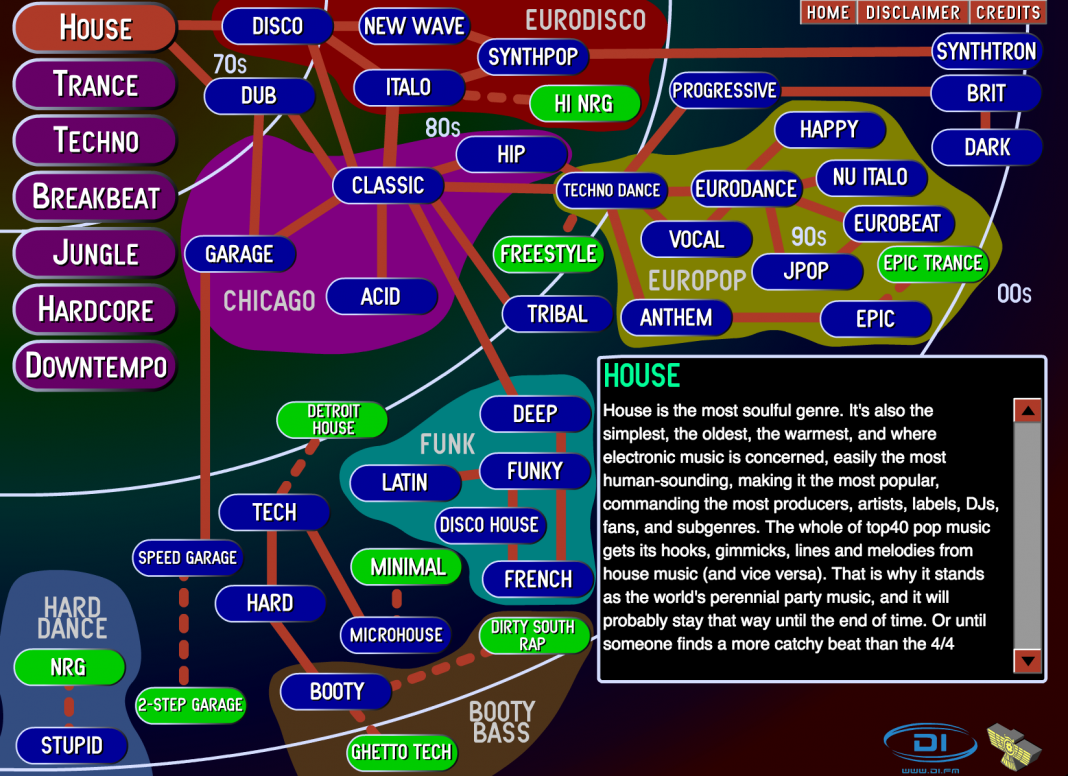
\includegraphics[width=\figSizeHundred]{ch02_dancemusic/figures/ishkur.png}
	\end{center}
	\caption[Ishkur's guide to electronic music.]{Ishkur's guide to electronic music.}
	\label{fig:ishkur}
\end{figure}

\section{House}

The act of going to a venue purely to dance and listen to recorded music carefully selected by a DJ existed well before the arrival what we now know as electronic dance music, as is clear from the disco era in the 1970s. Clubs such as “Paradise Garage” and “Studio 54” became focal points for the general public as well as artists living in New York, and were revered for their sound systems and resident music selectors. It was at these lengthy sessions that the cult of the DJ would nurture, with one of the most notable emerging being DJ Larry Levan. Levan would pioneer many aspects of what is now understood as the classic “DJ Set”, and was particularly celebrated for his ability to “read the crowd” - to adapt and change his sequencing and mixing depending on the mood of the audience of a given night. He was instrumental in developing the practice of remixing music, and in later years started to incorporate samplers and drum machines when repurposing older R\&B records for his dance floor.

The enduring legacy of disco left the most lasting impression on the city of Chicago, where it enjoyed heavy rotation in its venues long after its demise in other urban centres \citep{Reynolds2013}. Disco’s fading popularity meant that new releases were less forthcoming, inevitably leading DJs in the city scrambling to remix and update existing records à la Larry Levan, in order to stay fresh and current for audiences. One of Levan’s disciples, Frankie Knuckles, was a resident at the Warehouse club in Chicago, where his blending of regular disco and the electronic leaning Italo-disco from Italy (Giorgio Moroder would be its most notable export) soon became morphed and intertwined with his own bass lines and drum tracks \citep{Butler2006}. Eponymously, the name for this style was eventually shortened to become what is now known as ``house''.

Listening to classic house tracks, it is rooted unequivocally in a ``four on the floor'' regular 4/4 bass drum pattern, supplanted with synthesised claps and snares on the second and fourth backbeats, indicative of the equipment it was built on: the infamous TR-808 drum machine (\figref{fig:roland})\citep{Blashill2002}. Owing to its disco roots, house music is often described as the most “soulful” of dance music styles, in no small part due to syncopated baselines based around the root and the fifths, with short, jazzy electric piano style vamps providing harmonic context for catchy vocal hooks.

\begin{figure}
	\begin{center}
		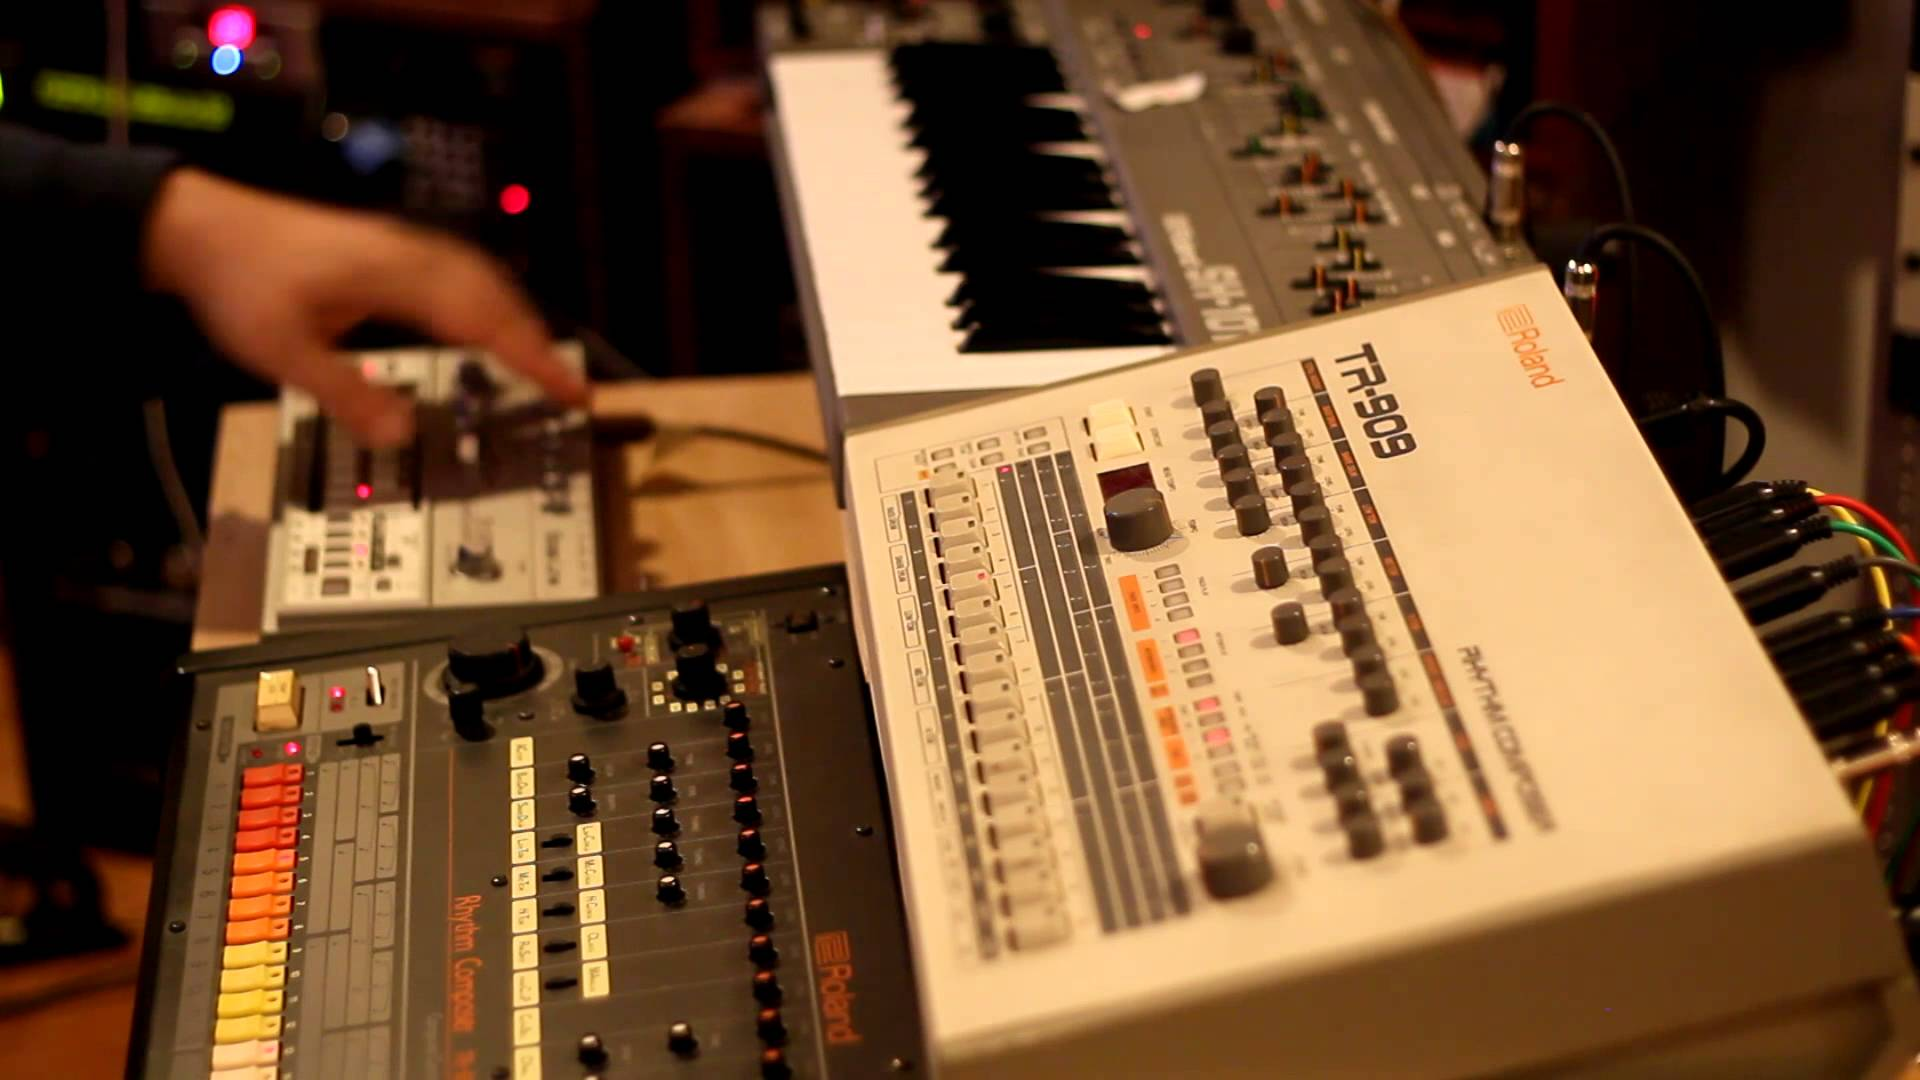
\includegraphics[width=\figSizeHundred]{ch02_dancemusic/figures/roland.jpg}
	\end{center}
	\caption[Roland electronic music instruments]{The Roland Tr-303 (top-left), TR-808 (bottom-left) and TR-909 (bottom-right) (Image from Synth Mania)}
	\label{fig:roland}
\end{figure}

Towards the latter half of the 80s, the Chicago house scene gave way to a more stripped back, harder sound known as acid house. A classic example of how a singular misuse of technology can redefine an entire genre, acid house built its entire identity out of another Roland product, this time the TR-303 bass synthesiser \citep{McLeod2001}\footnote{\url{https://youtu.be/TLQwwtjtiY4}}. The production team “Phuture” discovered that by constantly modulating the frequency cutoff and resonance parameters of the bass pattern, they managed to create a frantic new “squelching” bass sound that both diminished the roles of traditional layering techniques using keys and vocals and emphasised the value of new production tricks, deliberate or accidental \citep{Vitos2014}. 

Acid house was to prove most influential, however, when the first records made their way across the Atlantic to the United Kingdom. In London and Manchester clubs such as Shroom and the Hacienda (the latter owned and managed by the label Factory Records along with its flagship group New Order \citep{hook2009hacienda}) heavy rotation of acid house tracks triggered what would eventually become known as the “rave” movement. The rave movement was centred around large, spontaneous but entirely unlicensed gatherings focussed on marathon sessions of dancing to acid house and, much to the chagrin of authorities, consumption of club drugs such as MDMA. Rave culture would reach its peak during 1988-1989, culminating in what is now referred to as the “Second Summer of Love” \citep{Gore1997}. High profile coverage in the tabloid newspapers caused `moral panic' \citep{Martin1999}, and demonised and politicised rave music, so much so that the controversial 1994 Criminal Justice Act included a clause granting police full authority to halt any event involving the “emission of a succession of repetitive beats” \citep{gilbert1997soundtrack} \footnote{Veteran duo Autechre (who could hardly ever be accused of basking in repetitivity) in response released \textit{Anti} EP containing a track ``programmed in such a way that no bars contain identical beats'', with the warning: ``...we advise DJs to have a lawyer and a musicologist present at all times to confirm the non-repetitive nature of the music in the event of police harassment'' \citep{Atkinson2007}} .

\section{Techno}

Around the end of the 1980s a similar musical development to house was burgeoning in the city of Detroit, Michigan. Detroit was already a complicated city with a chequered past; it was here that Motown records was formed, with artists like Marvin Gaye producing some of the most defining soul music of the 1960s and early 1970s. The name Motown, a portmanteau of motor and town,  acknowledges Detroit  as the “motor city” - once the epicentre for the American car industry in the early part of the 20th century. Towards the second half of the century this once booming complex collapsed due to increased overseas competition from countries like Japan and national economic decline. Today the graveyard of abandoned factories in downtown Detroit serve as a bitter reminder of these greater years \citep{Sicko2010}.

The continued de-industrialisation, suburbanisation and the eventual relocation of the legendary soul label Motown Records to Los Angeles in 1972 had a devastating impact on the cultural output of the urban centre. But bubbling under the surface in Detroit's suburbs three middle class African American high school friends, known as the “Belleville Three”,  were planting the seeds for what would become techno. Juan Atkins, Derrick May and Kevin Saunderson were obsessed with sci-fi, technology and futurism, and raised on a diet of George Clinton funk and Italo-disco coupled with frequent visits to Chicago for injections of house, however it is widely acknowledged that their greatest influence would be German electronic group Kraftwerk \citep{Pope2011}. This was largely due to a seminal local radio show hosted by Charles Johnson a.k.a. “The Electrifying Mojo”\footnote{\url{http://daily.redbullmusicacademy.com/2015/05/electrifying-mojo-feature}}, mixing artists like Prince with European new wave, italo-disco and krautrock \citep{Reynolds2013, Sicko2010}. But it’s no coincidence Atkins, May and Saunderson latched on to Kraftwerk forthright. Kraftwerk’s albums revealed a group enamoured with the themes of transport, progress and movement, from the Beach Boys inspired ode to German motorways  “Autobahn”, to the pan-European romanticism of rail travel on \textit{Trans-Europe Express} \citep{Albiez2010}. This naturally resonated with the Detroit trio’s formulating ideas of Afro-futurism, against the backdrop of a city once so intertwined with the machinery of transportation and automobilisation.

Like Chicago house, Detroit techno was constructed and produced using the tools available at the time, inevitably the gamut of Roland’s drum machines and bass sequencers, coupled with whatever other synthesisers and sampling equipment was on hand. Tempo markings are also similar than house, most frequently in the 110 to 140 bpm range. So what distinguishes techno from house then? Techno at least, is considered more minimal and mechanical than house, less rooted in the more soulful influences of disco and soul as artist May points out:  

\blockcquote[]{collins_schedel_wilson_2013}{``\textit{House still has its heart in 70s disco; we don’t have any of that respect for the past, it’s strictly future music. We have a much greater aptitude for experiment.}''}

There is a driving energy to techno that discriminates it from house tracks, the tonality is often more dissonant and ominous. Kraftwerk style vocoder driven vocals and titles such as “No UFO’s” [sic] and “Time Space Transmat” highlight the futurist, utopian themes and aesthetic that makes this era of Detroit techno idiosyncratic. 

Techno would go full circle and transport itself back to Germany, where clubs such as Tresor and Berghain in the capital of Berlin soon became shrines for techno lovers from around the world. Berlin takes its techno very seriously. Tresor and Berghain are housed in huge, imposing former power plants\footnote{Suffice it to say, Kraftwerk is the German word for “power station”} and factory warehouses, with the latter recently receiving the same tax status\footnote{\url{http://pitchfork.com/news/68211-berghain-declared-high-culture-venue-by-berlin-court/}} as other more historic cultural centres such as opera and concert halls \footnote{Berghain’s legal representative successfully argued that “concertgoers may achieve a similar intoxicating effect from a Mahler symphony as from a DJ set”}. These industrial settings have moulded and shaped the sound of techno further, just like acid house did with its softer earlier incarnations. German techno sounds big, heavy and dark. Kick drums are brutal, relentless and reverberated, the reliance is more on metallic, machinery inspired sound design than on any easily discernable pitched, melodic or harmonic material. \cite{Nye2013} has also traced this trajectory of evolution (or perhaps devolution?) and observes a marked `minimalism' of the sound compared to its trans-Atlantic predecessor.

\begin{figure}
	\begin{center}
		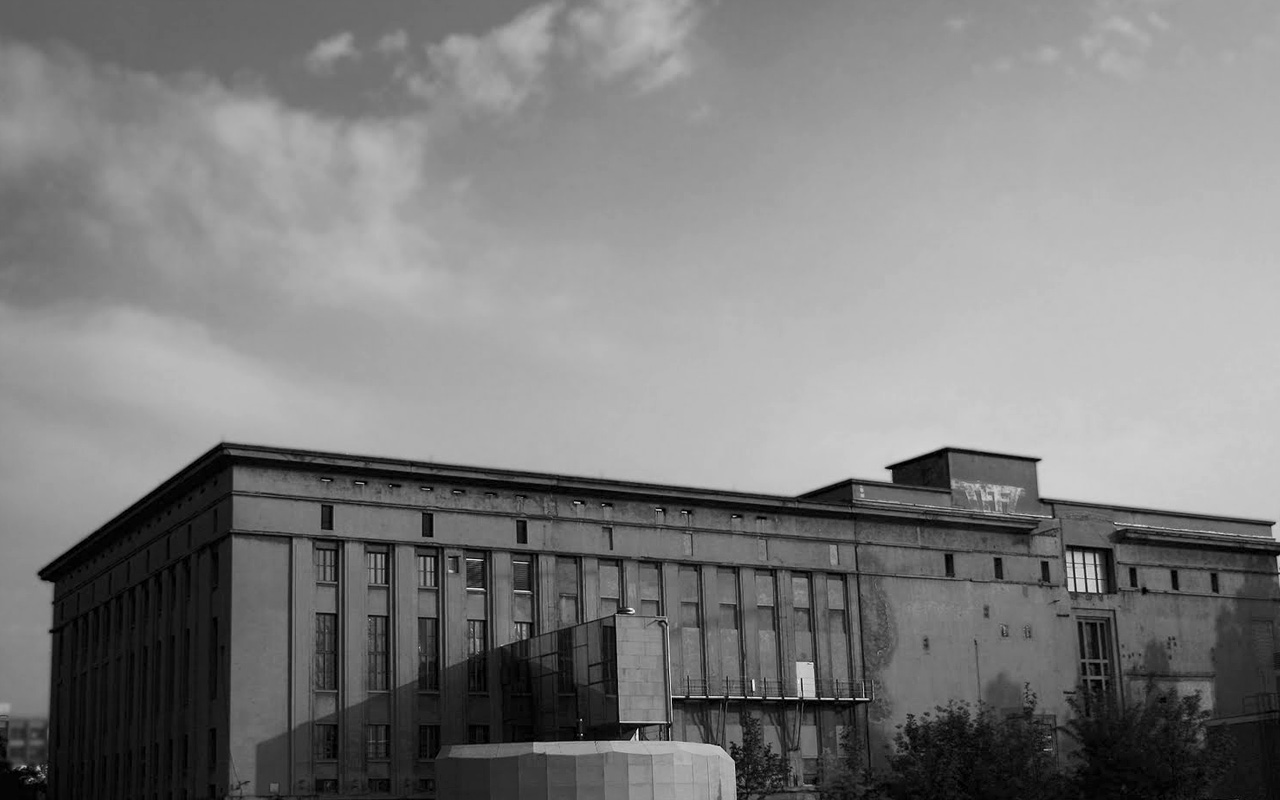
\includegraphics[width=\figSizeHundred]{ch02_dancemusic/figures/berghain.jpg}
	\end{center}
	\caption[Berghain club in Berlin]{Berghain club in Berlin, housed in a former power plant. Image from Resident Advisor.}
	\label{fig:roland}
\end{figure}

In a fitting closing observation, it is interesting to note that Kraftwerk, many years later, have acknowledged their influence on techno as well as the cultural duality shared by these two cities seemingly so far apart: on their track “Planet der Visionen” the refrain is \textit{"Detroit/Germany/We're so electric"}.

\section{Jungle and Drum ‘n’ Bass}

As the innocence and hope of rave dream started to disentangle and disintegrate in an increasingly volatile post-Thatcherite Britain, a radically new sound rose up from the ashes. Jungle, hardcore or drum ‘n’ bass drew its inspiration from two rather disparate influences. Firstly, in New York in the 1970s, DJ Kool Herc realised that by sequencing two copies of the same record, and looping the isolated “break” section - a short passage of drum soloing from funk and R\&B records - he could create a 5 minute performance for the purposes of “break” dancing and for an MC (Master of Ceremonies or Microphone Controller) to rhyme over \citep{Smith2000}. 

As such, Kool Herc essentially devised the underpinnings of a musical framework for emerging hip hop culture and rap music. Hip hop, as opposed to say, house and techno, is \textit{sample-oriented} music, meaning that manipulation of existing recordings of audio are utilised far more than raw signal generating synthesisers. Jungle builds on hip hop’s sampling aesthetic and heavy reliance on breaks but takes it to completely new extremes. With the development of sophisticated hardware production tools such as the Roland MPC (Music Production Centre) and, subsequently, the personal computer, endless new possibilities for complex and finely grained sample manipulation was within reach of homegrown bedroom producers.

Jungle’s other roots is the direct result of United Kingdom’s past as a colonial power. Migration from the Commonwealth Caribbean island of Jamaica\footnote{In fact, DJ Kool Herc was born in Kingston, Jamaica, and would have been exposed to dancehall culture before emigrating to the United States at the age of 12 \citep{Chang2007}.} to London brought with it reggae, dub music and sound system culture in general. Dub reggae was already a technology-centred form of music way before dance producers began twiddling with Roland gear. Engineers like Lee Scratch Perry would take instrumental versions of reggae tracks and remix them live using a slew of mixing desk tricks and exaggerated drenching of outboard effects (most prominently using the Roland Space Echo), blurring the lines between what constitutes the boundaries of the producer, performer and composer. Dub was performed at dedicated events with massive sound systems and MCs, somewhat prototypically anticipating central aspects of hip hop and rave. 

Just as reggae’s basic rhythm inverted the traditional downbeat and upbeat pattern of rock, jungle completely upends the traditional symmetry and repetition of house/techno dance music. Equally, just as the combined rhythm section of the bass guitar and drums (referred to as the \textit{riddim}) takes a more pivotal role in reggae, the drums in jungle and drum and bass are easily the most dominant element. As Simon Reynolds observes:

\blockcquote[]{Reynolds2013}{``\textit{In jungle, the rhythm is the melody; the drum patterns are as hooky as the vocal samples or keyboard refrains}''}

Where jungle departs greatly from its spiritual predecessor however is the actual arrangement of rhythmic patterns and its tempo. Reggae songs like chugs along typically around the 80 BPM mark; jungle can easily reach BPMs of almost double that\footnote{And wreaking havoc on BPM detectors!}. Drum production in jungle music is based around creating endlessly complex and dizzyingly intricate resequencing and reinterpretations of breakbeats. Many breakbeat samples have been used over the past decades, but the most infamous and enduring undoubtedly remains the “Amen Break”, a short 4-6 second drum solo on the song ``Amen Brother" by 1960s R\&B group The Winstons \citep{Collins2007a}. Along with an excerpt from ``Funky Drummer" by James Brown, they hold the contentious titles of being the most sampled breaks in music, contentious because the artists in question have received little or no royalty payments for its reproduction.

\section{Warp Records and \textit{Artificial Intelligence}}

By the early 1990s electronic dance music was already maturing to a point where it began to look inward at itself in reflection and contemplation. After a long night of hedonism, ravers were not likely to listen to more punishing dancefloor oriented beats but rather sought out a more subdued, laid back sound to match abating moods.

Warp Records, a Sheffield-based techno label anticipated this development and decided to capitalise on the emerging trend in a defining series of compilations known as \textit{Artificial Intelligence}. Looking at the green cover of the first release, it depicts a lone automaton comfortably seated in an armchair, facing a stereo system and a shelf of vinyl records. The intention is clear: this is not music for dancing, and as if the image wasn’t enough, the subtitle below proclaims “Electronic Listening Music From Warp”. The \textit{Artificial Intelligence} series would go on to release seven other albums, proving highly influential in the trajectory of dance music and bolstering Warp Records’ reputation as a bastion for “groundbreaking music” and, later on, branching into video and cinema. They cleverly managed to usher in an era of album format electronica, thus securing their longevity by doing away with the single release model responsible for the short lifespan of many a prior dance music imprint.

\begin{figure}
	\begin{center}
		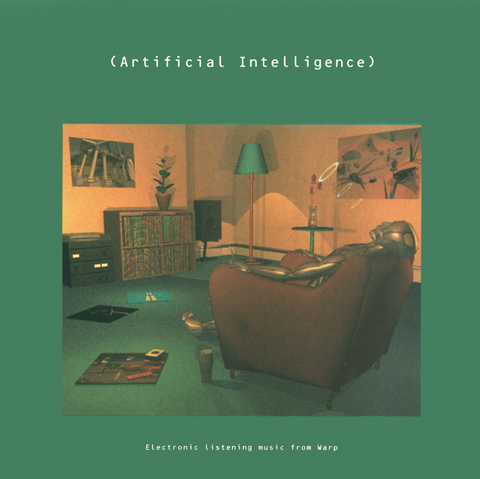
\includegraphics[width=0.6\textwidth]{ch02_dancemusic/figures/warp.jpg}
	\end{center}
	\caption[Cover sleeve for \textit{Artificial Intelligence} (Warp Records)]{Cover sleeve for Warp Records' \textit{Artificial Intelligence}. Image from Warp.net.}
	\label{fig:roland}
\end{figure}

The early music released by Warp Records was swiftly retitled by fans as \acrfull{idm}, a catch all label that largely grew out of discourse between members of Usenet forums discussing rave music to describe “music that moves the mind, not just the body” \citep{Alwakeel2009}. Immediately the term was controversial, even by those who would be considered its most respected innovators.  The problem with the IDM label is that it not so much describes a sound, rather than a collective ethos that just simply eschews conventional dancefloor geared sounds and production aesthetic. Richard D. James (Aphex Twin) takes further umbrage at the supposed elitist connotations it conveys:

\blockcquote[]{Haworth2015}{``\textit{I just think it's really funny to have terms like that. It's basically saying 'this is intelligent and everything else is stupid.' It's really nasty to everyone else's music. It makes me laugh.}''}

Comparing Warp Records’ stalwart roster of Aphex Twin, Squarepusher, Autechre and Boards of Canada under this umbrella term proves how divisive and varied the actual musical output is. Scottish duo Boards of Canada blend an uneasy mix of woozy, tape modulated hip hop beats with nostalgic samples from old VHS cassettes on their classic albums \textit{Music Has The Right To Children} and \textit{Geogaddy}. This is light years removed from, for example, the increasingly cold, angular and austere precision that has characterised most of Autechre’s exhaustive back catalogue. Starting out with reasonably symmetric post-techno repetitions and melodic analog synthesis on albums like \textit{Incunabula} and \textit{Tri Repetae}, Autechre’s music has become more abstract and hard to pin down over time, owing as much sonically and aesthetically to Greek composer/theorist Iannis Xenakis as to any Detroit pioneer.

Mostly this transformation has arisen out of their shifting and maturing use of technology. Albums like \textit{Confeld} betray a pair of experimentalists enamored with algorithmic composition, particularly using the Max/MSP environment. Regarding their continuing use of interactive software in live contexts they have described\footnote{\url{https://www.residentadvisor.net/features/2756}} how their processes differ from more traditional laptop performances: 

\blockquote{``\textit{I mean, there's no actual music "there"—it's not like we make music, then use the system to replay it in new ways. The system itself is making the music each time, it's all about the capabilities of the system dictating what the music's like}''}

Indisputably however, it is Aphex Twin who has become the bona fide poster boy for Warp Records and IDM as a whole. The Cornish producer started out with two double albums exploring ambient techno and beatless ambient music on \textit{Selected Ambient Works 85–92} and \textit{Selected Ambient Works Volume II} respectively. Later albums delved further into extreme recontextualisation and interpretation of earlier jungle and drum ‘n’ bass - often referred to by its detractors as “drill ‘n’ bass” due to its harshness and intensity - culminating in his most personal and broad record: \textit{Drukqs}. Over two discs, this album leaps from Satie-esque furniture music on “Avril 14th” to musique concrète (``Gwarek2'', ``Gwety Mernans''), as well his many brutally complex post jungle workouts on tracks like “Vordhosbn” and “Mt Saint Michel + Saint Michaels Mount”. 

Richard D. James and his labelmates, with their supposed ``intelligent" take on dance music, managed to win much favour and legitimacy in contemporary and art music circles. The 2006 compilation \textit{Warp Works \& Twentieth Century Masters }mixed pieces of Aphex Twin and Squarepusher pieces alongside performances of Ligeti, Varèse and Cage, while London-based chamber ensemble Alarm Will Sound have recorded careful and faithful arrangements of Aphex Twin and Autechre on albums such as  \textit{A/Rhythmia}. What’s striking about listening to these experiments is how natural and appropriate they sound compared to many forced and kitsch attempts at orchestrating rock music for instance.\footnote{Perhaps this is more of a personal aversion - I played in orchestras in my youth and I absolutely loathed those light medley arrangements of Beatles and Beach Boys that sanctified all the dangerous elements of rock `n' roll.}

As suggested in the introductory chapter, this has been an attempt to provide a short familiarisation with dance music from cultural, musicological and, in places, sociopolitical perspectives. It was not my intention to be exhaustive nor authoritative; I understand there are countless subgenres of dance music that I have omitted for the sake of brevity and enthusiasts and experts alike may take umbrage with those I've chosen to retain and my summaries of them. What I would hope is that the reader gains a flavour of my understanding of dance music and appreciate its scope for our forthcoming study.
\cleartorecto%!TEX root = ../thesis_a4.tex
\chapter{Generative Symbolic Music}
\label{chap:symbolic}

\section{Introduction}

As long as computers have been available, a curiosity has prevailed as to whether computers are capable of being creative \citep{Cardoso2009}. Indeed the multidisciplinary area known as computational creativity \citep{Boden1998, Wiggins2006, Boden2009a, Boden2009, Colton2012} gathers researchers from artificial intelligence, cognition, philosophy and the arts, in order to investigate this lofty aspiration. In the wider sphere of computer music, algorithmic composition \citep{Jacob1996, Fernandez2013} endeavours to construct programs\footnote{Although most texts introducing algorithmic composition will be at pains to emphasise that algorithmic composition - in the context of some systematic application of rules for composing, like in Mozart's Dice game or in twelve-tone technique and serialism - in fact predates the computer.} that could automatically generate (or help generate) works of music for human listeners. With some composers, the goal is to model style conforming compositions \citep{Cope1987, Cope1991} so convincingly that they pass some interpretation of the Turing test \citep{Ariza2009}, while, others accept algorithmic composition for what it is - a different type of music, hence accepting all its limitations or possibilities, or as Pease puts it:

\begin{figure}
	\begin{center}
		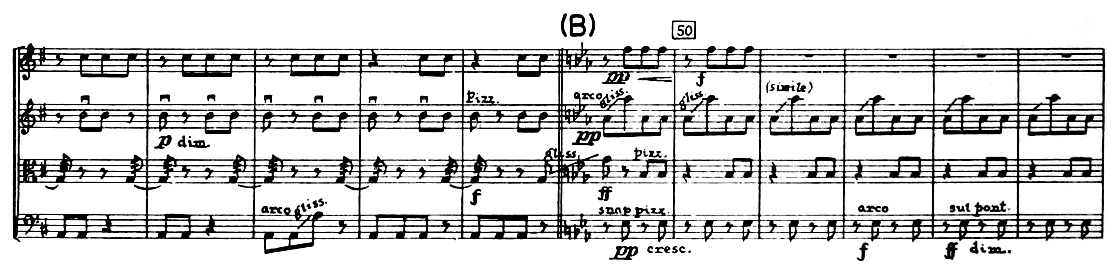
\includegraphics[width=\figSizeHundred]{ch03_symbolic/figures/illiac.jpg}
	\end{center}
	\caption[Excerpt from the \textit{Illiac Suite} (Lejaren Hiller)]{Excerpt from the Illiac Suite by Lejaren Hiller. Image from \cite{Morgan2015}}
	\label{fig:illiac}
\end{figure}

\blockcquote[]{Pease2011}{``\textit{Turing Test is largely inappropriate for the purposes of evaluation in Computational Creativity, since it attempts to homogenise creativity into a single (human) style}''}

In the early days of computer music composition, digital synthesis was only in its theoretical infancy, so algorithmic composition experiments typically involved generating some form of symbolic medium for later realisation as something audible. For instance, composers such as Hiller used supercomputers to generate a numerical computer score (\figref{fig:illiac}) which was then transcribed manually to staff notation and performed by a live string quartet \citep{Hiller1979}. Iannis Xenakis, in his treatise \textit{Formalized Music} \citep{Bradshaw1973}, explains how he harnessed supercomputer capability to generate large stochastic distributions that generated parameters for written compositions also to be realised by live performers. It is interesting to hear  how Xenakis calls attention to the role that computer programs play in \textit{assisting} him in his creative practice, rather than holistic generation of entire works\footnote{There are obvious parallels to be drawn here with Autechre's statement regarding their live work in \chapref{chap:dancemusic}.}:

\blockcquote[]{Cope2000}{``\textit{the computer has not actually produced the resultant sound; it has only aided the composer by virtue of its high-speed computations''}}

Later, with the advent of General \acrshort{midi}, music-oriented programming environments such as Max, \acrshort{pd} and OpenMusic were used to procedurally control note information and parameters of external hardware synthesisers and samplers automatically. One of my prior works \citep{Nuanain2014} explored tangible table-top interfaces modelled on the Reactable \citep{Jorda2005} for interactive control of real-time compositional algorithms, in a bid to expand the controller space offered by other real-time composition practitioners such as Karlheinz Essl \citep{Essl2014}. These experiments comprised a collection of Max/MSP patches that sent streams of algorithmically generated \acrshort{midi} control information to a virtual bank of synthesisers and samplers hosted in a \acrshort{daw}.

\section{Algorithmic Composition Techniques}

Programmatic techniques employed in algorithmic composition range from the very rudimentary (simple random number generators) to very sophisticated arrangements of agents borrowing from artificial intelligence. Algorithmic composition systems can be qualified as stochastic (the output is unpredictable), deterministic (the output is predictable) or hybrid, where one or more aspects of the system are determined.

There exists a wealth of conceptual approaches exist for algorithmic composition that have fallen in and out of flavour over the years. We summarise key ones here that we feel are representative of the current state of the art and pertinent to the arguments put forth within the thesis. For a thorough treatment of historical methods for algorithmic composition we suggest consulting the Computer Music Tutorial \citep{Roads1996} or surveys reported by \cite{Fernandez2013} and \cite{Papadopoulos1999}.

\subsection{Stochastic Processes}

Stochastic processes are largely concerned with strategic applications of probabilistic procedures. When composers defer some aspect of their creative activity to some element of chance they are invoking a stochastic process; whether this be the flip of a coin to choose which section to enter in a large musical structure or using a random number generator to select pitch values on their synthesiser, for example.

\subsubsection{Probability Distributions}

Composers using random processes in a serious way (like Hiller and Xenakis) naturally gravitate towards methods of influencing the outcomes in some systematic manner. They  utilise probability table lookups to shape a specified probability distribution geared towards a desired musical elemental goal. Most computer music oriented software environments have some sort of facility for creating such distributions interactively, and in fact Max/MSP provides a visual table object for drawing distributions explicitly. They can be used to create standard mathematical distributions such as linear, bell-shaped, skewed etc., and \textit{The Computer Music Tutorial} \citep{Roads1996} gives derivations for many of them in the chapter dealing with algorithm composition. \cite{Ames1990a} also gives insight into similar statistically grounded modes of composition.

Sometimes a more musically specific distribution is required. Using the example of a probability distribution influencing the outcome of pitches available from the 88 notes of a conventional keyboard, we could envisage a distribution that only allows notes from the major scale, and favours the root, fourth and fifth as prevalent in many Western musical idioms.

Thinking further about this, if an analysis can be performed on a suitable set of representational data (such as a score, \acrshort{midi} file or features extracted from audio), the distribution of pitches in the scores of Chopin or based on pitch histograms in a selection of Javanese Gamelan recordings, one may surmise a very elemental manner of encapsulating the notion of style within a composition system. 

Instinctively however, the fundamental feature lacking is any information about the appropriateness of the pitches given the surrounding context and overall trajectory. One extremely applicable method of addressing this is through the use of Markov processes.

\subsubsection{Markov Processes}
\label{sec:markov_chains}

A Markov chain is a probabilistic system that satisfies the Markov property of memorylessness. It consists of a set of discrete states with each state having an associated probability weighting of moving to every other state in the system. At any point in discrete time, the probability of a future event is solely determined by the current state (or a few states depending on the \textit{order}) of the system without knowledge of the preceding past events. This can be expressed more formally by \eqnref{eq:markov}.

\begin{equation}
  \label{eq:markov}
  \begin{gathered}
P=(X_{t+1}|X_{t}=x_{t},X_{t-1}=x_{t-1},...,X_{0}=x_{0}) \\
=(X_{t+1}|X_{t}=x_{t})
  \end{gathered}
\end{equation}

where $X_t$ is the state occupied by the state machine at time $t$ in its discrete history. To build a Markov chain, a transition matrix is defined that determines the probability of moving from one state to each other, often by analysing or modelling some real world examples. The order (i.e. the number of states in the right hand side of the second line of \eqnref{eq:markov}) of this transition matrix is the number of states that are considered when determining the probability of the next state. A first order Markov chain, for example, considers the probability of jumping to the next state based on the current state, while a second order chain would use the current state and the previous state in determining where to move to next.

Markov chains have enjoyed widespread application in simulating stochastic processes, and in music they are employed routinely for algorithmic composition \citep{Fernandez2013, Eigenfeldt2009, Jorda2016}. A simple Markov chain for generating notes in a particular style could be achieved by building a transition matrix from the number of times the root note of a scale transitions to every other note in a corpus of \acrshort{midi} files. This could be expanded to include a concurrent transition matrix that contains probability of transition of observed note rhythm values. Some of our colleagues in GiantSteps have also addressed drum pattern generation with a system of Markov Chains derived from style specific corpora addressing various strands of electronic dance music \cite{Jorda2016, Gomez-Marin2016}.

With The Continuator, \cite{Pachet2002} has garnered considerable exposure in the application of Markov chains in call and response style interaction with a human performer\footnote{And we shall see later \cite{Biles1994} achieves something similar with his means of ``trading fours'' with a real-time listening \acrshort{ga}.}. The allure of Pachet's work has been its satisfaction of a number of Turing style tests \citep{Pachet2008}. More recently its successor \acrshort{ai}, FlowMachines \citep{Pachet2008a}, has stirred up great publicity\footnote{\url{http://www.flow-machines.com/tag/flow-machines-press/}} with its generation of the first artificially intelligent pop song\footnote{With the caveat being a human wrote the lyrics and arranged and performed the final work.}. In their usage of Markov chains, they have acknowledged their facility for modelling temporal phenomena such as music, but emphasise the challenge in reconciling them for interactive control. To solve this they have proposed a class of hybrid Markov chain system that includes elements of constraint satisfaction, known as an \acrfull{emc} \citep{Pachet2011}, proving fundamental for chord generation in the Continuator \citep{pachet2001finite, barbieri2012markov}.

Music generated by Markov Chains can be deceptive in their `low-level' convincingness but it is still very localised in contrast to larger human-composed works with careful macroscopic attention to form. As \cite{Collins2011a} comment on The Continuator: ``it is fundamentally parasitic on the duration data passed to it'' and has ``difficulty with longer-term structure''.

To combat this the composer can increase the order of the Markov system - thereby lengthening the `memory' of consideration in the state machine - or similarly lengthening the size of the snippets of symbolic music atoms that are to be used for chaining, but the results still baulk at a point. As Roads observes when studying hymns generated with a Markov chain by \cite{Brooks1993}. 

\blockcquote[]{Roads1996}{``\textit{...low-order chains generated meandering, random melodies, while high-order chains consist of parts of the original hymns spliced together, such as the first half of one hymn crudely spliced onto the second half of another hymn. This can be explained as a strong probabilistic tendency towards coherence over several notes that is broken suddenly by a more unlikely event, at which point a new coherent melody starts''}}

Jordà concurs in his own evaluation of his own compositions for live computer music generating jazz chord progressions. 

\blockcquote[]{Jorda1991}{``\textit{Markov music usually presents a very short correlation, sounding much better over brief fragments, than over long ones.}}

With these criticisms in mind, maybe this makes the case for hybrid systems that can scale with the demands of larger scale computer music composition. By invoking a layered approach with multiple agents perhaps taking the role of a meta-composer for the purposes of coherent musical form. In fact Eigenfeldt does talk about this in the context of musical meta-creation \citep{Eigenfeldt2016}, and prior to that defines some mechanism that is rudimentarily capable of doing something to that effect. In \textit{GESMI} - the Generative Electronica Statistical Modeling Instrument \citep{Eigenfeldt2013} - for example, expert annotations of aspects of electronic dance music including subdivisions into section labels such as `lead-in', `intro', `verse' and `breakdown' are used by a genetic algorithm to dictate higher-level surface features while Markov chains generate localised motifs as usual. In another work \citep{Eigenfeldt2016a}, another high-level meta-agent defines a series of parametric curves that affect overall compositional aspects such as speed, density and complexity that are adhered to by other reactive generative agents.

\subsection{Formal Grammars}

Continuing with the goal of epitomising style in computational models and generative procedures, we turn to another approach that tries to achieve this using language theory. Formal grammars have long been used to interpret hierarchical relationships in syntactical aspects of language \citep{Chomsky1957}, and are an essential element of compiler theory and programming language design \citep{garshol2003bnf, wirth1996compiler}.

The controversial debate continues as to whether music can really be considered a universal language \citep{Campbell1997, Savage2015} but, nevertheless, applying formal grammar theory has enjoyed considerable utility in the systematic analysis of musical concepts as well as generative tasks. In his famous Harvard lecture series ``The Unanswered Question''\footnote{\url{https://youtu.be/MB7ZOdp__gQ}}\citep{bernstein}, the conductor Leonard Bernstein pondered whether music could be characterised using Chomsky’s formal generative grammars \citep{Chomsky1957}. Subsequently inspired by this hypothesis, musicologist Fred Lerdahl and linguist Ray Jackendoff \citeyearpar{lerdahljackendoff} joined forces to compile ``A \acrfull{gttm}'', one of the most complete compendiums to classify Western classical music using grammar techniques. A dense and complex work, it nevertheless provides a methodological framework for understanding what we hear when we listen to common practice works. The metrical structure rule for instance, positions beats in a tree structure such that it accounts for the natural strong and weak grouping of accentuation that occurs at different metrical levels of pulse as can be seen in \figref{fig:gttm}.

\begin{figure}
	\begin{center}
		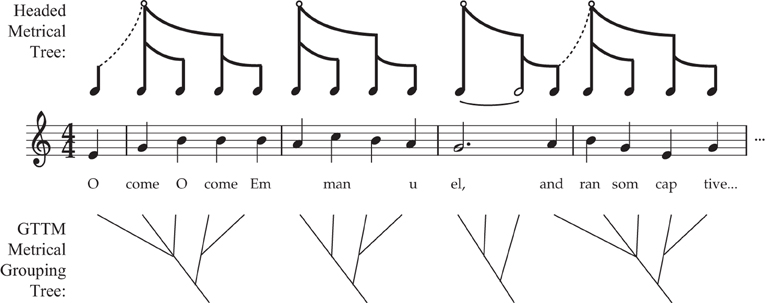
\includegraphics[width=\figSizeHundred]{ch03_symbolic/figures/metricalhierarchy.jpg}
	\end{center}
	\caption[Generative Theory of Tonal Music Metrical Hierarchy Grouping]{\acrshort{gttm} Metrical Hierarchy Grouping. Image from \cite{Fitch2013}.}
	\label{fig:gttm}
\end{figure}

Lerdahl and Jackendoff’s \acrshort{gttm} represents, as Roads suggests, an “analysis of syntactic structures” where musical events are parsed into syntactic hierarchical structures \citep{Roads1996}. Conversely he contrasts the analytical viewpoint with the synthetic: “starting from a specification of large-scale syntactic structure fill in the details for each of these structures”.

The \acrshort{gttm} essentially comprises an analysis or distillation of style, the style loosely being common practice era Western art music. Composer David \cite{Cope1991} has, using his musicological expertise, performed a similar analysis of music from this era, but with a more finely grained focus, initially on Bach chorales. More importantly the primary goal of this analysis is to inform the eventual synthesis of style. Cope distills his \acrfull{emi} \citep{Cope1987} process into three critical stages that mirror Roads’ observations regarding duality of musical application involving formal grammars. In any case he identifies them as:

\begin{itemize}
	\item Deconstruction - segmentation and analysis of existing representative work
	\item Signatures - identifying demonstrative motifs and traits that distinguish a stylistic genre or composer’s proclivity
	\item Compatibility - recombine deconstructed elements into fresh cohesive and coherent musical works
\end{itemize}

Controversy aside, what Cope perhaps highlights most of all is the role of the designer in building computer composition systems. As is evident, building a software that can achieve the output of \acrfull{emi} is no easy feat, demanding a Bach scholar with knowledge of the nuances of voice leading, counterpoint, as well as computational musicological skills that include awareness of \acrshort{ai} methods and programming in \acrshort{lisp}\footnote{\acrfull{lisp} is a programming language with a long association in the field of \acrshort{ai} and by extension, computer music \citep{taube1991common, taube2004notes, assayag2006computer}.} for example. On a more philosophical note, it should follow that the designer then must impart some aesthetical footprint on works produced by such systems. So if we can hear which part reveals a piece to be Bach, then which part is the designer? Which part is the computer? 

Cope has available 5000 examples of computer generated Chorale in \acrshort{midi} format on his website, and has continued his experiments to include more larger scale works extending into the common practice era and beyond (e.g. Mozart and Mahler \citep{Muscutt2007, cope2009hidden}). His efforts have had an enduring and frequently contentious impact not only in academia \citep{Wiggins2008} but also in the public’s psyche; by addressing well known and easily identifiable stylistic goals (verifiable once again with musical style Turing tests)   he establishes clear markers in the sand for what is achievable with algorithmic composition. 

\subsection{Genetic Algorithms}


\acrfull{ga}s, as introduced in seminal works by \cite{Holland1975} and \cite{Goldberg1989}, are a class of heuristic search solutions modelled on the theory of natural selection \citep{koza1992genetic, Srinivas1994}. Along with artificial neural networks and emergent systems they can be classified as a biologically inspired computing method that employs some well understood  process from natural sciences to help solve a more complex computational task \citep{Mitchell1998}.

In a \acrshort{ga}, potential solutions to a conceptual problem are encoded with a genome string representation (usually with binary bitstrings). Using a series of genetically-inspired operations such as crossover and mutation these strings are ``evolved'' until their quality reaches a satisfactory level, hence performing an implicit search sweep over a large space of candidates.  Central to the operation of evolutionary algorithms and determining genomic quality is the \textit{fitness function}, which determines the individuals that are allowed remain in successive populations. Naturally effective representations are important to ensure effective use of evolutionary algorithms - a badly defined encoding can skew the performance towards that of exhaustive search. 

Several logical stages are involved in a genetic algorithm which we now discuss in turn:

\paragraph{Initiation:}
To initiate the search space, a population of individuals is generated randomly, though some rules-based procedures can assist in “kick starting” a faster, more informed process.

\paragraph{Fitness:}
The fitness function is a problem-dependent evaluation procedure that determines the suitability of the candidate solution to the problem. There are no hard and fast rules as to what determines a “good” fitness function; this is - along with specifying an appropriate representation - part of the craft in evolutionary algorithms. An alternative is to use an interactive fitness function, which involves using an external agent (typically a human critic) to determine suitability of candidates. 

\paragraph{Selection:}

In accordance with Darwinist theory, the fittest $f$ individuals are more likely to be chosen for reproduction and generation of future population members. This is in essence probabilistic, and one popular selection schema is roulette wheel selection, or fitness proportionate selection. Here, the probability assigned to an individual is given by the proportion of the individual fitness to the overall population (\eqnref{eq:roulette}).

\begin{equation}
\label{eq:roulette}	
p_{i}=\frac{f_{i}}{\sum_{i=1}^{N}f_{i}}
\end{equation}

Where $p_i$ is the probability of individual $i$ being chosen and $f_i$ is the fitness of that individual.

Roulette wheel selection derives its nickname from being akin to reserving a portion of a spinning roulette wheel in a casino. In \figref{fig:roulette} this can be graphically compared to truncation selection which simply selects the top \textit{N} members from the list when sorted by fitness.

To create the offspring, genetic operators are applied to the parent individuals, the two most common being:
\begin{itemize}
	\item \textit{Crossover} - pick a splice point s in the bit strings of the genome, take bits 0 - s from parent A and combine with bits s - n from parent B.

	\item \textit{Mutation} - a certain (small) portion \ of the newly generated population is chosen at random and within these individuals a random bit is flipped. As in nature, the mutation procedure allows for genome sequence combinations that may not occur using crossover alone.
\end{itemize}

\begin{figure}
	\begin{center}
		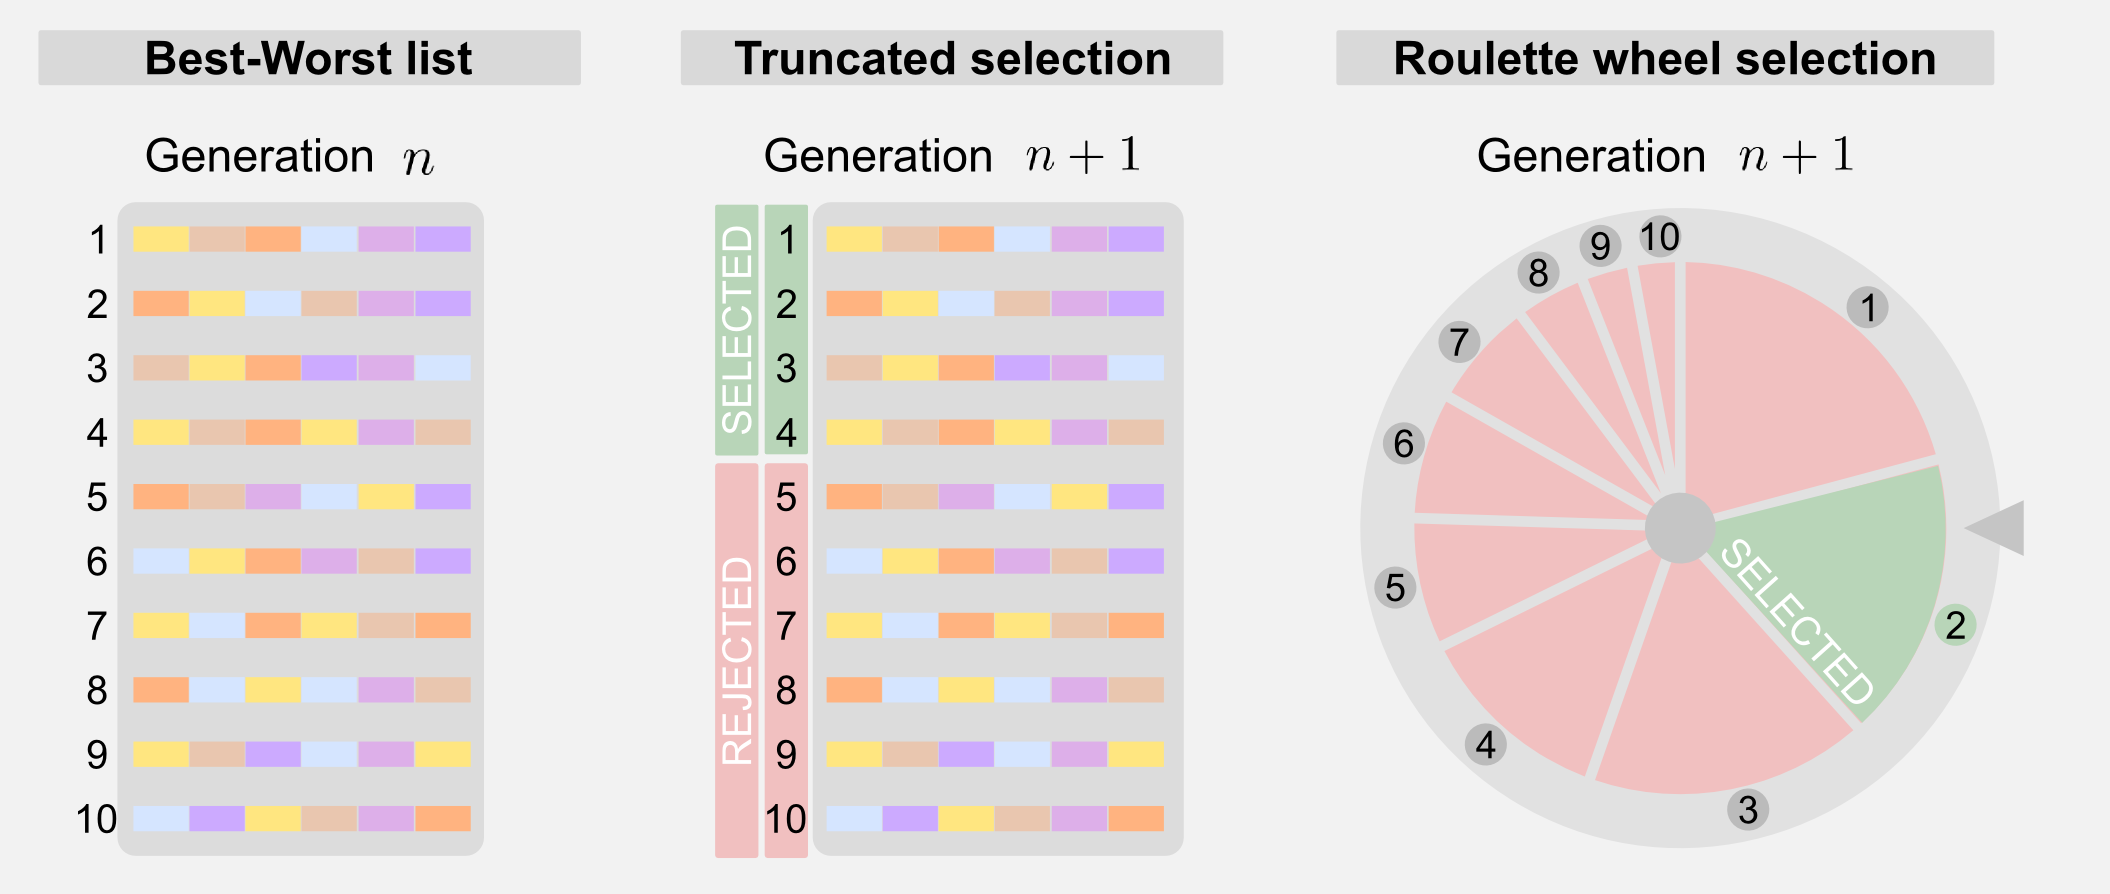
\includegraphics[width=0.9\textwidth]{ch03_symbolic/figures/selection.png}
	\end{center}
	\caption[Truncation and Roulette Wheel Selection in a Genetic Algorithm]{Sorted best to worst list of candidates (left). Truncated selection of top 4 candidates (middle). Probabilistic roulette wheel selection (right). Image from Dissecting Reinforcement Learning\footnote{\url{https://mpatacchiola.github.io/blog/2017/03/14/dissecting-reinforcement-learning-5.html}} }
	\label{fig:roulette}
\end{figure}

\subsubsection{Evolutionary Music}

Genetic algorithms have certain qualities that make them an attractive choice for artificial creativity, so much so that there exists an ardent strand of research devoted entirely to what has come to be known as “evolutionary art” \citep{Romero2008, McCormack2013} and furthermore, evolutionary music \citep{Miranda2007a} .

Undoubtedly, they are an elegant and easy to comprehend search heuristic, and the underlying concept of generating a bunch of candidate solutions that hopefully converge on some ideal is appealing to the process of an artist. So too is the idea of the interactive fitness function, where humans can directly appraise potential candidates subjectively. Naturally this is the most optimal method aesthetically but the slowest method performance-wise, especially in highly temporal domains such as sound and vision, where it is typically referred to as the “fitness bottleneck” \citep{Todd1999, Biles2001, Gartland2003}. 

One of the most well known applications of genetic and evolutionary algorithms to music has been Al Bile’s GenJam system \citep{Biles1994,Biles2002,  Biles2003, Biles2007} which interactively generates streams of monophonic solo melodies in bebop jazz style.  It is a classic example of an interactive genetic algorithm \figref{fig:genjam}, where the composer considers himself a “mentor” to the system, actively incrementing and decrementing fitness of generated phrases as they arise in real time from the program. Internally, the genetic algorithm actually maintains two populations of structures. The phrase population contains a list of indices that reference measures in the measure population. A measure is considered a short eight-note phrase of \acrshort{midi} pitch values, with special symbols for silence and held notes.  One of GenJam's unique feature is the ability to “trade fours” with the live performer whereby pitch detection is performed on a monophonic input source, and the phrase that is altered using genetic modifiers is played back to the performer.

\begin{figure}
	\begin{center}
		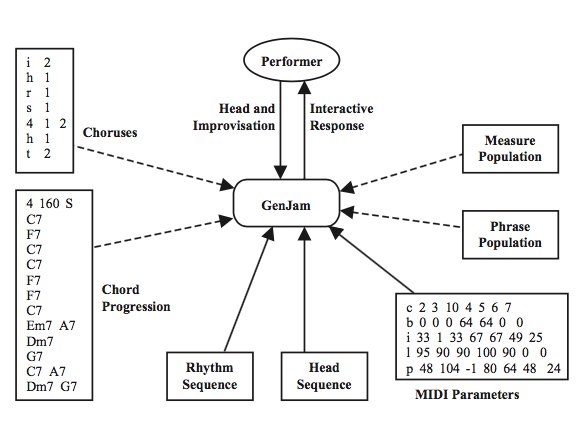
\includegraphics[width=0.8\textwidth]{ch03_symbolic/figures/genjam.png}
	\end{center}
	\caption[GenJam Interactive Architecture]{GenJam architecture with different populations and interaction with performer. Image from \cite{Miranda2007a}.}
	\label{fig:genjam}
\end{figure}

Now that we have seen a glimpse of basic methods for symbolic algorithmic composition, we will begin our study of symbolic generation focussing on rhythm using computer processes. We will turn our attention to some key works presented in the literature and describe a new method of target-based rhythmic pattern generation using genetic algorithms. An evaluation will unearth the feasibility of such methods for rhythm pattern generation and the limitations that can be identified that informs a revision of the models used.\

\section{Symbolic Rhythm Generation}

\subsection{Representation}

As evident from such designs as Léon Theremin's `Rhythmicon', the Wurlitzer `Sideman' and Raymond Scott's `Rhythm Synthesizer'\footnote{The Rhythm Synthesizer would sow the seeds for a later drum machine called `Bandito the Bongo Artist' which would be used on the ground-breaking proto-ambient record \textit{Soothing Sounds for Baby}\citep{Collins2011a}} \citep{Tindale2009, Malmberg2010, Arar2013}, there have been many esoteric early incarnations at building and incorporating drum computers, with these strange experiments in the early half of the 20th century paving the way for a more unified design aesthetic emerging towards the latter half. 

\begin{figure}
	\begin{center}
		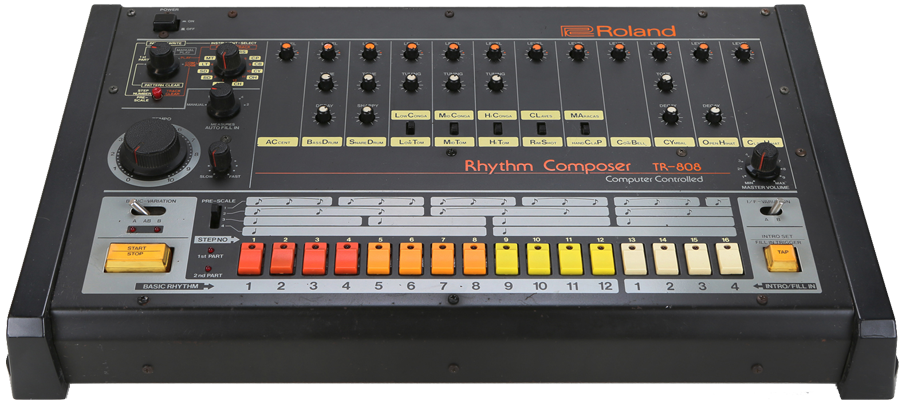
\includegraphics[width=0.75\textwidth]{ch03_symbolic/figures/tr-808.png}
	\end{center}
	\caption[Roland TR-808 Drum Machine]{Roland TR-808 Drum Machine}
	\label{fig:tr-808}
\end{figure}


Most notably, one can not underestimate the profoundly influential impact of the designs of Ikutaro Kakehashi and the Roland Corporation on the shape and history of electronic music and its culture. Originally considered a commercial flop due to its perceived inauthentic synthesis of natural drum sounds, the Roland TR-808 drum machine (\figref{fig:tr-808}) has since become the icon of post 1980s dance oriented music, and its distinctive synthetic character soon became synonymous with techno and house styles \citep{theberge1997any}.

The TR-808 was intended as a rhythm accompaniment device, and as such was designed to be easy to use by non drummers. Its operation involved selecting the required drum sound and inputting a pattern using a row of 16 buttons corresponding to discrete points in time based on a global tempo. This binary based approach has continued on into computer music platforms and virtual instruments. 


This simple but concise metaphor of representing basic patterns has been adapted also in the literature dealing with the musicological study of rhythm, most notably by \cite{Toussaint2013} who has carried out considerable research into geometric approaches for rhythm analysis and similarity. The binary input mechanism is clearly a convenient medium for transferring to computational analysis while remaining descriptive and intuitive for human comprehension.  \figref{fig:reps} shows how a particular rhythm can be represented in a number of different symbolic representations including traditional staff notation forms.

\begin{figure}
	\begin{center}
		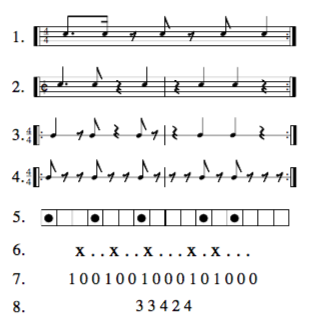
\includegraphics[width=0.55\textwidth]{ch03_symbolic/figures/reps.png}
	\end{center}
	\caption[Different Forms of Symbolic Rhythm Representations]{Different Forms of Symbolic Rhythm Representations (Image from \citep{Toussaint2003}}
	\label{fig:reps}
\end{figure}

The fifth form in the figure, the most familiar to drum machine interfaces, is referred to as the \acrfull{tubs}. It is considered easier by many ethnomusicologists in depicting and grasping complex rhythmic structures such as polyrhythms not typical in Western Art Music \citep{nzewi2008musical, koetting1970analysis}.  

Continuing in this line, other representational schemes have been devised in attempt to represent rhythms in a more holistic and natural manner, given its cyclical and hierarchical centricity. Often rhythms are portrayed using a circle or necklace system with beats and onsets occupying geometric portions of the structure, as can be seen in \figref{fig:necklace}. These are frequently used to depict more complex rhythmic patterns that exist in African and Latin traditions, giving a different perspective and insight into their latent balance and symmetry.

\begin{figure}
	\begin{center}
		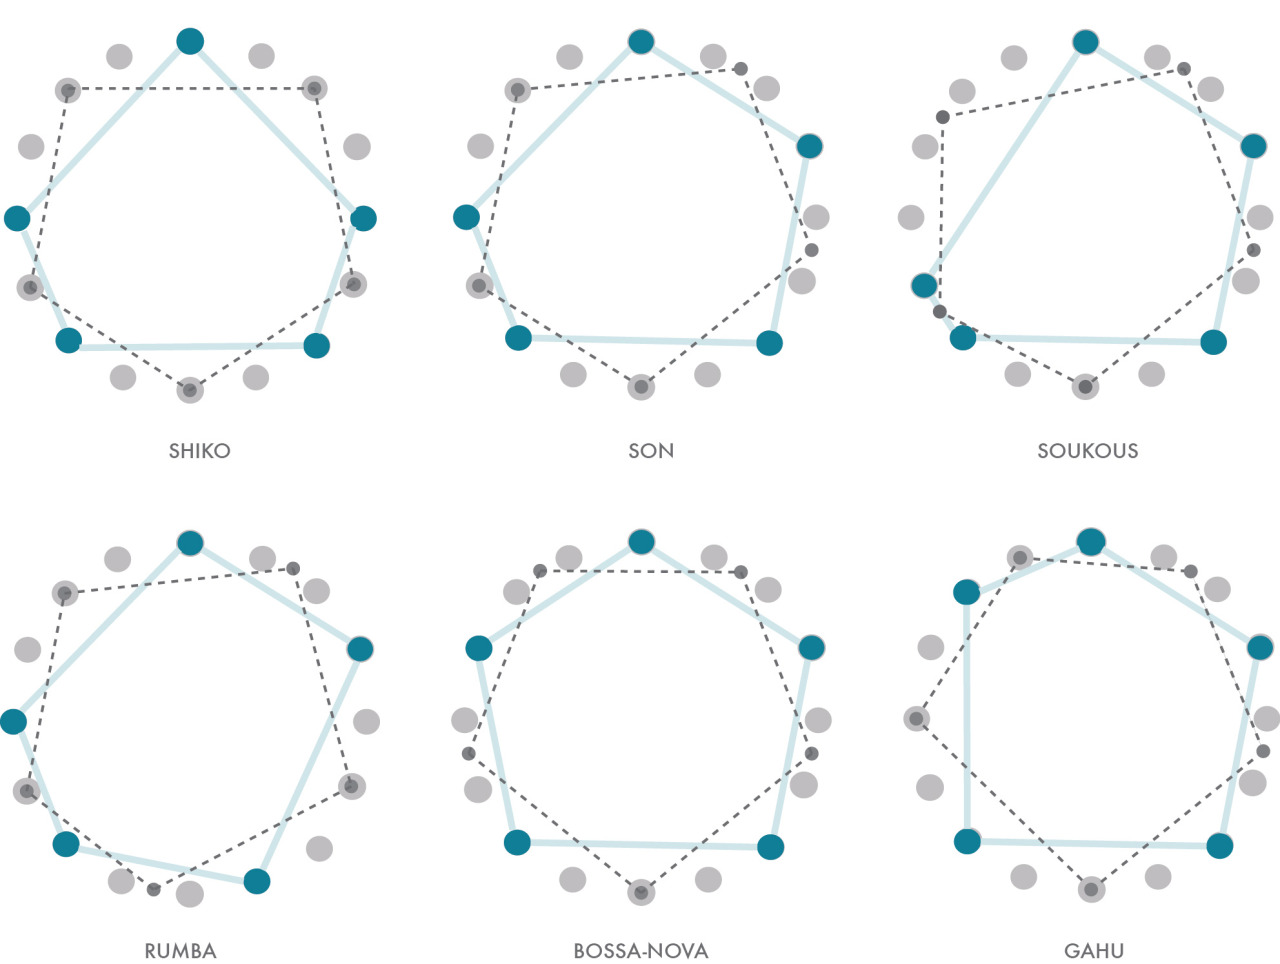
\includegraphics[width=\figSizeHundred]{ch03_symbolic/figures/necklace.jpg}
	\end{center}
	\caption[Necklace Depictions of Some Popular Rhythms.]{Necklace depictions of some popular rhythms.(Image from Ethan Hein\footnote{\url{http://www.ethanhein.com/wp/2015/beats-and-scales/}})}
	\label{fig:necklace}
\end{figure}

These circular representations have proved alluring for computer music practitioners, and a number of rhythm focussed applications have been developed exploiting this necklace paradigm. Xronomorph \citep{Milne2015a, Milne2016}, provides an environment for experimenting with rhythms that conform to mathematical properties of perfect balance and well-formedness. As a unified mobile application, Rhythm Necklace\footnote{\url{http://rhythmnecklace.com/}} is a visually appealing application for iPad for experimenting with geometrical approaches to rhythm generation.

\begin{figure}
\centering
\begin{subfigure}[b]{1.0\textwidth}
   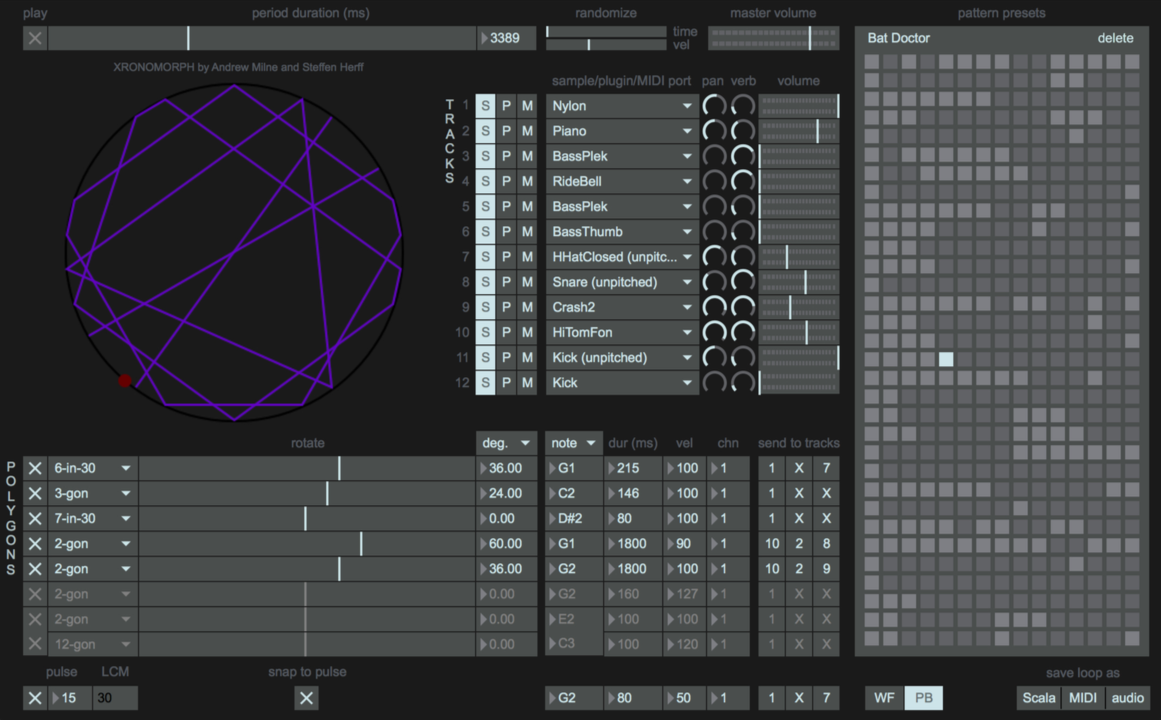
\includegraphics[width=1\linewidth]{ch03_symbolic/figures/xronomorph.png}
   \caption{}
   \label{fig:Ng1} 
\end{subfigure}

\begin{subfigure}[b]{1.0\textwidth}
   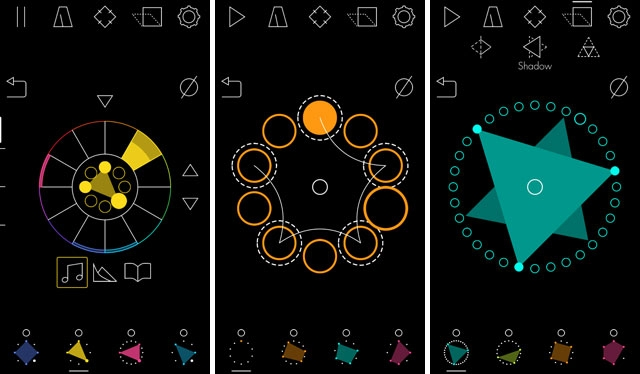
\includegraphics[width=1\linewidth]{ch03_symbolic/figures/necklace2.jpg}
   \caption{}
   \label{fig:Ng2}
\end{subfigure}

\caption[Two numerical solutions]{(a) XronoMorph Interface (Image from \cite{Milne2016}), (b) Rhythm Necklace App (Image from Ethan Hein\footnote{\url{http://www.ethanhein.com/wp/2015/rhythm-necklace/}})}
\end{figure}

\subsection{Measuring Rhythmic Similarity}

One of the primary tasks that has dominated symbolic rhythm study has been the formalisation of methods for measuring the degree of similarity between two rhythmic patterns. It was previously shown how natural rhythms can be distilled down to a very simple representational form suitable for computational analysis (and hopefully generative composition).

Obviously, there is a wealth of knowledge and systematic approaches for measuring similarity borrowing from information sciences when dealing with computer readable data, or in particular, strings. Methods of comparing strings, or string metrics, are an essential aspect of coding theory. Symbolic rhythmic study has adapted many of these metrics for its analysis and \cite{Toussaint2004} has summarised many of the key matching techniques. Superficially, we can take a distance measure, feed it some rhythms encoded as binary strings and do some basic normalisation/algebra to convert it to some degree of “similarity”.

The key question here is how do these objective information metrics compare with the cognitive human impression of similarity? With this very shallow abstraction of what a rhythm is, we must surely lose a great deal of latent information that undoubtedly must contribute to similarity perception; consider the influencing factors of accentuation, swing, timing imperfections, instrumentation, timbre, production, genre and surely, culture. 

Regardless, the foundations of understanding rhythmic similarity need to begin somewhere. We turn our attention now to methods of estimating similarity of simple binary string representations of rhythmic structures and discuss their relevance and application for generative purposes in a practical system in due course.

\subsubsection{String Similarity and their Application to Rhythms}

\label{sec:distance_measures}

\begin{figure}
	\begin{center}
		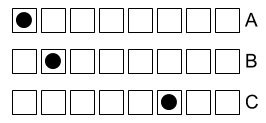
\includegraphics[width=0.45\textwidth]{ch03_symbolic/figures/hamming_comparison.png}
	\end{center}
	\caption[Hamming Distance Comparison]{Same Hamming Distance for Three Patterns}
	\label{fig:hamming_comparison}
\end{figure}

The primary advantage of the simple binary representation exemplified by the \acrshort{tubs} notation is its malleability for simple bit comparison and string analysis using common algorithms. We summarise a number of them here for clarification, but Toussaint  offers a more thorough synopsis of many of them and their application to rhythm.

\paragraph{Edit Distance:} The edit distance or Levenshtein distance is a widely-used measure of difference between two strings of information. It counts the number of insertions, deletions and substitutions required to transform one string into the other. The  Levenshtein distance between the two strings “kitten” and “sitting” for example returns 3, based on two substitutions and one addition. The edit distance can operate on strings of differing lengths, and is solved using recursion or dynamic programming techniques.

\paragraph{Hamming Distance:} The hamming distance counts the number of positions in which two equal length strings differ. A simple measure that is easy to compute for the machine and easily comprehensible for the human. Hence it is a restricted version of the edit distance, limiting itself solely to substitutions of symbols.

\paragraph{Swap Distance:} As \cite{Toussaint2013} notes, one of the problems with the edit distance and the Hamming distance is that they don’t capture the horizontal aspect of string similarity so well. In \figref{fig:hamming_comparison} for instance, comparing string A to string B and string C both return a distance of 2, even though comparing them horizontally they are clearly very different.

To this effect, Toussaint proposes the use of the swap distance, actually borrowed from similar computations that take place in the realm of bioinformatics, to capture the number of placewise shifts to make one string match the other. as he did in his study of African ternary rhythms \citep{Toussaint2003}. In the simple case of binary encoded rhythms with equal number of onsets or 1s - known as one-to-one mapping - the distance can be computed by summing the absolute differences in their indices \citep{Toussaint2016} - essentially the L1-Norm or ``Manhattan'' distance (\eqnref{eq:swap}) when considering element $a_i$ and $b_i$ from two strings $A$ and $B$.

\begin{equation}
\label{eq:swap}
	\mathcal{D}_\mathrm{S}(A,B) = {\sum_{i=1}^{N}|a_i-b_i|}	
\end{equation}

Of course natural rhythms can have different numbers of onsets and this does make computing swap like similarity considerably more complex. To handle this extended case of many-to-many, \cite{Diaz-Banez2004} have applied what is known as the directed-swap in their analysis of flamenco patterns, which stipulates, when comparing a pattern A with more onsets than pattern B that:

\begin{enumerate}
	\item Each onset in pattern A must move to an onset in pattern B.
	\item Every onset in pattern B must receive at least one onset from pattern A.
\end{enumerate}

In \figref{fig:swapvshamming}, we can see a visual comparison of the directed-swap distance as compared to the Hamming distance, as well as the different distance values they return. Conceptually, we can at least surmise that the directed-swap, with its ability to encode the horizontal displacement of onsets, should give a richer description of the similarity between two rhythms, such as embodying an impression of the syncopation introduced. if we were to move between both patterns.

\begin{figure}
	\begin{center}
		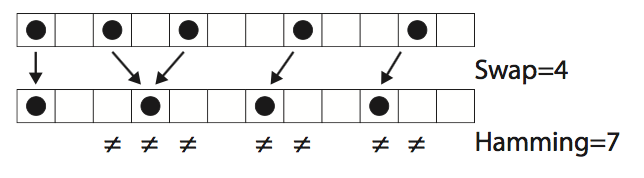
\includegraphics[width=0.65\textwidth]{ch03_symbolic/figures/swap_vs_hamming.png}
	\end{center}
	\caption[Swap and Hamming Distance Compared.]{Swap and Hamming Distance Compared.}
	\label{fig:swapvshamming}
\end{figure}

Actually computing this distance is also a more involved task. One proposed, which works in $O(n^{2})$ time, solution is to consider the task as finding the shortest path within a weighted acyclic graph, in the context of solving what is referred to as the restriction scaffold assignment problem in computational biology \citep{Colannino2005}.

\subsubsection{Other Symbolic Rhythmic Descriptors}

Here we summarise other useful descriptors pertinent to symbolic rhythmic analysis that are not exclusively based on determining similarity between two rhythms.

\begin{figure}
	\begin{center}
		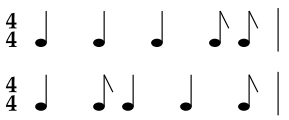
\includegraphics[width=0.4\textwidth]{ch03_symbolic/figures/ioi_comparison.png}
	\end{center}
	\caption[Comparing the identical IOI of Two Very Different Rhythms.]{Comparing the identical \acrshort{ioi} of two very different rhythms. Image from \cite{Dixon2004} }
	\label{fig:ioi_comparison}
\end{figure}


\paragraph{Inter-Onset Interval:} 
Rather than computing the difference between two rhythmic patterns based on the location of the onsets in time, the \acrfull{ioi} summarises a rhythm based on the time elapsed between each onset - or in other words the offset time \citep{Toussaint2013}. For example the clave son would be encapsulated in the string of time elapses as \{3,3,4,2,4\}, using some unit of reference such as 1 = ¼ note. 

Clusters of inter-onset intervals that occur periodically, at a regularly rate that can be quantified per unit time, are referred to by some in the literature as “temporal atoms” or tatum \citep{Bilmes1993, Sethares2007, Jehan2005}. Essentially we can consider the tatum of a score or recording as the fastest note division in which it is written or performed \citep{Sethares2007}. We shall learn later in Chapter 4 that the notion of tatum is important in extracting the tactus or, in musical information retrieval parlance, beat tracking. The computational task of beat tracking involves determining from a signal where a human is likely to tap their foot\footnote{Or more formally, the period at which the conductor swings their baton} when listening to music with a clearly discernable rhythm. 

While \acrshort{ioi}s are unedeniably one of the most important contributors to the impression of accent and pulse perception in music \citep{Parncutt1994}, they are not the most useful feature for comparing rhythms (which is what we are trying to achieve). Firstly as \cite{Dixon2004} correctly point out, two rhythms can have the same distribution of inter-onset intervals, but depending on the length of the notes themselves, the perception of their similarity can turn out to be very dissimilar indeed. In \figref{fig:ioi_comparison} the two rhythms have identical inter-onset intervals but the rhythm above is more typical of a Cha Cha rhythm while the rhythm below is clearly more syncopated and betrays more stylistically that of Rumba.


\paragraph{Chronotonic Distance:} 
Addressing the aforementioned shortcomings intrinsic to \acrshort{ioi}-based comparisons, \cite{gustafson1987new} expands the \acrshort{ioi} representation to a two-dimensional structure that also encapsulates interval time by the integrated area of the rectangle. This elegant depiction allows for clear visual comprehension of rhythmic patterns\footnote{Actually originally intended for scrutiny of rhythm within phonetic study} as we can see in \figref{fig:chronotnic} with the familiar Son. 

\begin{figure}
	\begin{center}
		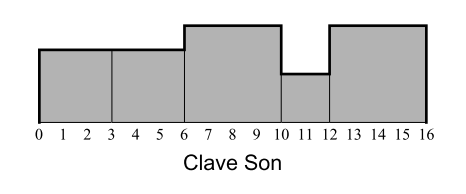
\includegraphics[width=0.65\textwidth]{ch03_symbolic/figures/chronotonic.png}
	\end{center}
	\caption[Chronotic Distance of Clave Son]{Chronotic Distance of Clave Son. Image from \cite{Toussaint2004}.}
	\label{fig:chronotnic}
\end{figure}

\citep{Toussaint2004} explains how to compare two patterns summarised by their chronotonic distances by treating them as probability distributions and using standard statistical distance measures. While he reports that the chronotonic distance edges past the swap distance based on the criteria of simplicity, goodness of fit, clustering, and ``ancestral'' rhythm generation (rhythms that serve as the seed for many many others), \cite{Guastavino2008} provide experimental evidence that the directed-swap correlates more highly with classically trained musicians’ perceptual impression of dissimilarity when comparing rhythms.

\section{A Genetic Algorithm based on Similarity}

The previous section introduced symbolic representation schemas for rhythm, and symbolic rhythm descriptors, with a particular focus on similarity measures between two rhythms. In this section we will explore how this systematic knowledge can be encapsulated in generative systems. We will begin with a glimpse into some existing relevant work, firstly looking at generative systems that deal with Toussaint style measures of similarity, followed by systems that use genetic algorithms to generate rhythm. Subsequently, we introduce our own proposed work that seeks to specifically merge perceptual measures of rhythmic similarity with genetic or evolutionary algorithms in a system we call GenDrum. We discuss the evaluation of the system and our conclusions that motivates our progression from the symbolic domain to direct content-based analysis and recombination of audio.

\subsection{Generative Rhythmic Systems}

\subsubsection{Generative Rhythmic Systems using Similarity Measures}

Publications dealing with generative applications of symbolic rhythmic similarity exist in the span of literature, but are not so widespread. The Hamming distance, with its easy comprehensible and computable qualities has naturally served a number of systems. \cite{Paiement2007} describe a paper centred around utilising the Hamming distance for generative modelling and prediction of simple rhythms trained in jazz and pop idioms. \cite{Vogl2017} present a tablet application that uses the Hamming distance combined with a restricted Boltzmann machine - a type of artificial perceptron neural network - trained on many drum styles from the Native Instruments Maschine\footnote{\url{https://www.native-instruments.com/en/products/maschine/}} collection. A modified extension has also been extended to database interpolation from that same collection in an earlier  publication \citep{Vogl2016}. Other distance metrics have been exploited less so, and we have found no instances of the directed-swap distance being used in generative tasks.

\subsubsection{Generative Rhythmic Systems using Genetic Algorithms}

Generative systems addressing rhythm with the means of \acrshort{ga} are more abundant. \cite{Eigenfeldt2006a} describes his Kinetic Engine as a software component that generates rhythms in general, not specific to drum sounds. His approach to fitness evaluation is perhaps a controversial one, but not uncommon in musical applications. As in Al Biles’ GenJam system, the role of fitness is simply eliminated. Thus the only real elements of genetic algorithms conserved are crossover and mutation. One may rightfully suspect that such a simplification renders the algorithm commensurate with a randomised search. Consequently a common solution used in such scenarios is to seed the initial population with a known dataset of good input. Another approach could be to embed some rule-based logic that restricts what type of candidates can be generated legally in the seeding process, as we carried out in \citep{Nuanain2014}.

\cite{Bernardes2010} approaches genetic drum pattern generation from the point of view of style emulation. Like Eigenfeldt, they do not incorporate a fitness function, but choose to perform prior analysis on user-supplied or preset MIDI files in a particular style. This process gathers a probability distribution of weighted possible onset times in a 16-step pattern. The population is then seeded with candidates that have patterns generated according to this distribution. 

A short paper by \cite{Horowitz2004a} suggests a multi-dimensional objective fitness function based on the combination of functional evaluations of syncopation, density, downbeat, beat repetition, etc.. Unfortunately the publication is rather scant on actual details regarding the implementation and evaluation of such a method. 

\cite{Kaliakatsos-Papakostas2013} also use the notion of a a target pattern in their evoDrummer software, and define their fitness function by determining what they refer to as divergence in terms of “mean relative distance” to a base rhythm. The distance is computed based on a set of 40 features extracted from patterns, including descriptions of density, syncopation and loudness intensity. Indeed this is perhaps the most related work to our proposed system. 

\subsection{Developing a Genetic Algorithm that can Generate Rhythm}

We set out to design a rhythmically motivated genetic algorithm that was capable of self-evaluation based on the similarity of the patterns it outputs compared to a user-provided seed target pattern. One can envisage this concept being extended to a system that can perform self-evaluation against a previously analysed dataset of patterns that conform to some notion of \textit{style}. 

This section introduces the tools we created in our research: SimpleGA, the genetic algorithm itself that can target the two well known music programming environments \acrshort{pd} and Max, and subsequently encapsulated in the real-time Max for Live instrument GenDrum. Max for Live is an extension of the Max programming environment inhabited in the popular \acrshort{daw} Ableton Live \citep{Manzo2015}. Ableton Live\footnote{\url{https://www.ableton.com/}}, in turn, is one of the most popular \acrshort{daw}s in the dance music community due to its non-linearity and grid-focussed arrangement of loops. 

We continue with a detailed discussion of the implementation of the distance measures and representational issues. Finally there is a description of the design of the experiment for evaluating the research.

\subsubsection{Software Implementation}

\begin{figure}
	\begin{center}
		\includegraphics[width=\figSizeHundred]{ch03_symbolic/figures/simpleGA.png}
	\end{center}
	\caption[SimpleGA Pure Data Help Patch]{SimpleGA Pure Data Help Patch}
	\label{fig:simplega}
\end{figure}

SimpleGA is a basic, general purpose genetic algorithm external object we developed for the Pure Data \citep{Puckette1997} and Max/MSP environments in C++ using the cross-platform Flext framework \citep{Grill} . It can handle binary, numerical and alphanumerical strings. A target string is supplied to the object and fitness is determined by measuring its distance to the generated strings using the Hamming or directed-swap distance as was introduced in \secref{sec:distance_measures}. Bang\footnote{The ``bang'' is a fundamental message in \acrshort{pd} and Max that basically means ``do your thing!'' \citep{winkler2001composing}} messages to the leftmost ``hot'' inlet causes the genetic algorithm to undergo a generational stage of evolution, then to output its fittest individual from the pool. \figref{fig:simplega} shows the help patch for the object with this functionality explained visually.

Next we created the GenDrum instrument, a Max for Live device that uses the SimpleGA genetic algorithm to create polyphonic drum patterns of synthesised kick, snare, hi-hat and crash/clap type sounds that emulate the style of a pre-conceived (by input from the user) pattern (\figref{fig:gendrum}). These four sounds are mapped onto a single 16-step row to create a 4x16 drum pattern matrix as is evident in the figure. The operation of the instrument is intended to be as simple as possible. The user inputs a desired pattern into the pattern matrix and assigns this as the target pattern. New target patterns can then be generated by clicking on ``Get New Pattern''. This assigns the best candidate in the current population to the grid and reports its fitness in the number box. In the yellow number box a target fitness can be issued to the genetic algorithm and clicking ``Accelerate!'' will increase the speed of the algorithm until it reaches this target. Patterns that increasingly approach perfect fitness now emerge from the algorithm, repeating and contrasting with the target pattern through repeated stages of \acrshort{ga} evolution.

The instrument also attempts to provide some visual feedback on the evolutionary process using a type of force-directed graph. The fittest individual from each population is represented as a node with its fitness determining the size and distance in relation to the target individual.

\begin{figure}
	\begin{center}
		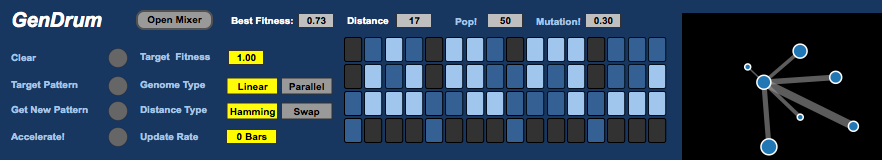
\includegraphics[width=\figSizeHundred]{ch03_symbolic/figures/gendrum.png}
	\end{center}
	\caption[GenDrum Main User Interface]{GenDrum Main User Interface}
	\label{fig:gendrum}
\end{figure}

\subsubsection*{Algorithm Details}

\textit{Linear vs. Parallel Operation}

As the previous section explains, the instrument is intended as a fully functional drum machine, and hence is polyphonic with the possibility of multiple sounds concurring in time. As seen in the literature, similarity studies are predominantly focused with examining monophonic patterns such as the single sound clave son\footnote{The clave son is a two bar measure of either a 3-2 or 2-3 pattern that is integral in many forms of latin dances \citep{Sethares2007}.}. How we deal with the polyphonic implications in our research is outlined here.

Our first naive implementation of the genetic algorithm converts the 4x16 drum pattern matrix into a single “linear'” 64-digit binary string. Evidently this is a simplistic ``brute force'' approach that does not explicitly take into account any musical or perceptual aspect of the application. Specifically it does not embed any knowledge about the constituent sounds and the separation between them in the genome string. Essentially, we’re treating it as a single sound 64-step pattern, with crossover and mutation happening at the halfway point between the first 16 bits of the kick and snare pattern and the second 16 bits of the cymbals/crashes. 

Another approach is to force some kind of logical separation between the different polyphonic timbres in the pattern. By assigning a separate instance of the genetic algorithm to each timbre an overall mean fitness can be derived from the individual outputs. This we implemented and labelled as ``parallel'' mode. Since the genome pattern length is now split from one single 64-bit string to four concurrent 8-bit strings, the time it takes for the genetic algorithms to reach the target fitness is considerably reduced. Some tweaking of the parameters is required to reduce this convergence time and maintain a healthy level of diversity. Setting the population size parameter to 30 and increasing the mutation rate parameter to between 20\% to 40\% has been found to work well in our experience. \figref{fig:genetic} shows the flowchart and design of the GenDrum instrument and it's encapsulation of the SimpleGA \acrshort{ga} in the aforementioned linear and parallel configurations. Next we turn our attention to the distance measures used to derive the fitness function of these genome patterns.

\begin{figure}
	\begin{center}
		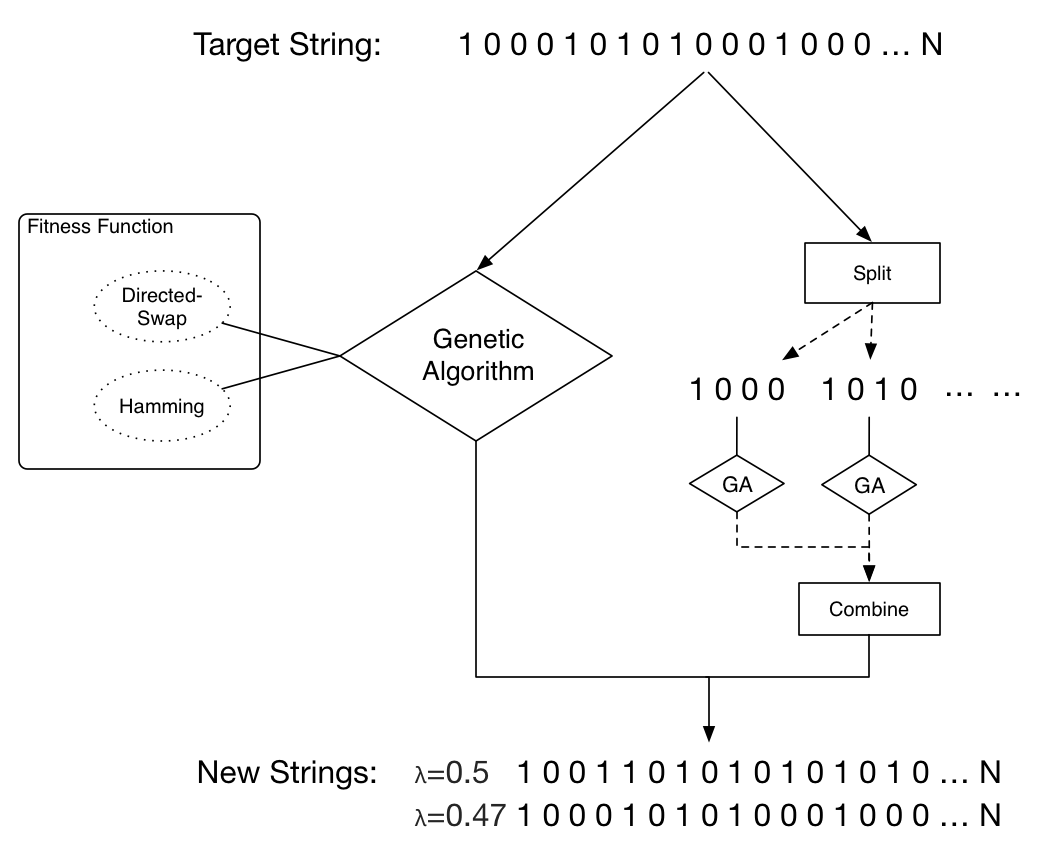
\includegraphics[width=0.8\textwidth]{ch03_symbolic/figures/ga_algorithm.png}
	\end{center}
	\caption[Genetic Algorithm Flowchart]{Genetic Algorithm Flowchart. The target string can either be fed to one single \acrshort{ga} (left) or split by timbre, processed by 4 parallel \acrshort{ga}s then recombined (right).}
	\label{fig:genetic}
\end{figure}

\textit{Hamming Distance}

In the review of the state of the art, we referenced how Post and Toussaint have surveyed the effectiveness of the edit distance in determining rhythmic similarity between two binary patterns \citep{Post2011}. Recall that the edit distance allows for insertion, deletion and substitution of symbols within the string. A simplification can be made if operations are restricted to substitutions only, and string lengths are equal (as is always the case in our representations) in which case it becomes the Hamming distance. 

To derive a fitness function using the Hamming distance (\eqnref{eq:fitness_hamming}, using the $\oplus$ exclusive OR operator to determine where the two binary strings are not equal), the number of positions where the two strings $a$ and $b$ match are counted and then divided by the total string length (64 for the linear string and 8 for each string in the parallel implementation). 

\begin{equation}
\label{eq:fitness_hamming}
	f=\frac{1}{N}\sum_{i=1}^{N}a_i \oplus b_i
\end{equation}

\textit{Directed-Swap Distance}

\label{sec:directed_swap}

The Hamming distance takes into account the correct positional scores between two patterns, but it does not give any indicator as to how different a pattern is in terms of the horizontal displacement. Intuitively one would think this horizontal displacement would reflect the important phenomenon of rhythmic syncopation. For example there may exist two different patterns with equal distance, but one pattern has more onsets aligned closer to the original pattern or exhibit a similar distribution of the strong and weak beats in the bar. For these reasons, we decided to test also the directed-swap distance metric as described by \cite{Diaz-Banez2004} in the study of flamenco rhythms, with the hopes that it better captures the spatial comparison between the our generated patterns and the target.

\begin{figure}
	\begin{center}
		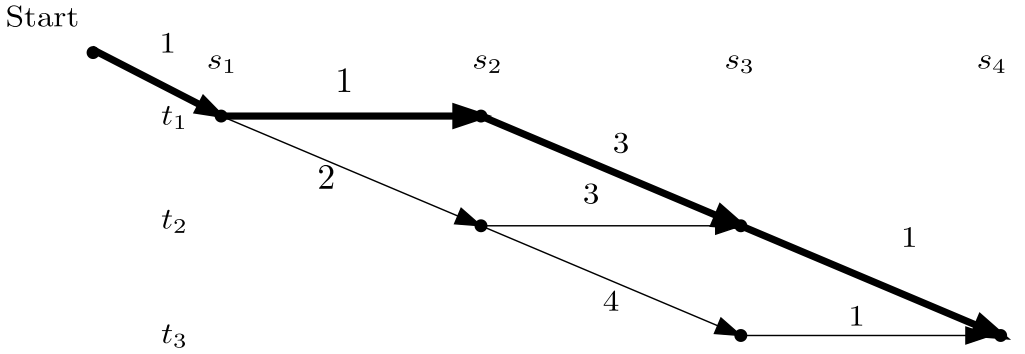
\includegraphics[width=0.75\textwidth]{ch03_symbolic/figures/shortest_path.png}
	\end{center}
	\caption[Solving the Directed-Swap Distance Graph for Two Strings]{Solving the directed-swap distance for strings $A=\{0,2,7,12\}$ and $B=\{1,4,11\}$. Image and example taken from \cite{Colannino2005}}.
	\label{fig:dijkstra}
\end{figure}

Since no implementation existed for the algorithm proposed by \cite{Colannino2005}, we implemented it ourselves, using the Dijkstra implementation in the Boost C++ graph library \citep{Siek2002} to compute the final distance\footnote{\url{https://github.com/carthach/SimpleGA/blob/master/SwapDistance.cpp}}. The derivation and proofs are described at length in their article \citep{Colannino2005} but the basic steps are as follows:

\begin{enumerate}
  \item Convert the two binary rhythms under scrutiny to two sets of indices respectively. For example the pattern $A = \{0, 0, 0, 1, 0, 1, 0, 0\}$ would reduce to the index vector $A = \{3, 5\}$.
  \item Construct a weighted directed acyclic graph from two index vectors $A$ and $B$ by firstly creating the set of vertices $v_{i,j}$ where $1 \leq i \leq |A|$ and $1 \leq j \leq (i+|B|-|A|)$.
  \item For each $v_{i,j}$ add an edge to $v_{i, j+1}$ with weight $|b_{i}-a_{j+1}|$, and an edge to $v_{i+1, j+1}$ with weight $|b_{i+1}-a_{j+1}|$, if $v_{i, j+1}$ and $v{i+1, j+1}$ exist.
  \item Create a start note and add an edge from that node to $v_{1,1}$ with weight $|s_{1}-t{1}|$.
  \item The directed-swap distance is given by the cost shortest path through the graph, solvable with Dijkstra's algorithm (\figref{fig:dijkstra}).
\end{enumerate}

\subsubsection{Operation and Performance}

One way to measure the performance of a genetic algorithm is to plot the fitness values it outputs over a succession of generations. In \figref{fig:genetic} we can see the best fitness and average fitness for all possible configurations of the genetic algorithm over 100 generations. Notice that the linear string representation causes convergence on the target within 40 generations. Notice also that the parallel representation converges prematurely in areas of local maxima, particularly using the swap distance. This can be alleviated through some encouragement of diversity by tweaking the population size and mutation rate.

\begin{figure}
	\begin{center}
		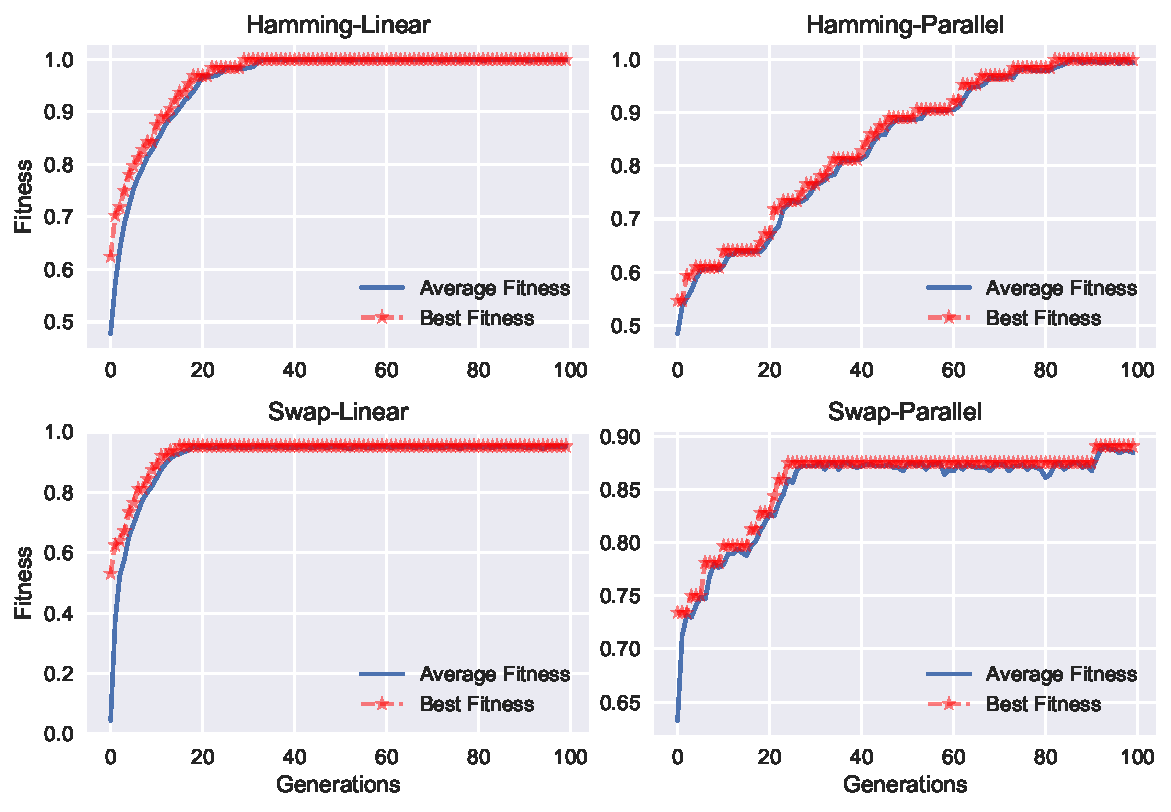
\includegraphics[width=\figSizeHundred]{ch03_symbolic/figures/best_average_fitness.pdf}
	\end{center}
	\caption[Fitness Plots for the Various Configurations of the Genetic Algorithm]{Fitness Plots for the Various Configurations of the Genetic Algorithm}
	\label{fig:genetic}
\end{figure}

\subsection{Listener Evaluation \& Discussion}

When evaluating this research and its resulting tools, our goals were to investigate:

\begin{itemize}
	\item The overall correlation of distance with perceived experience.
	\item Comparing the impact of the Hamming distance versus the directed-swap distance on the perceived experience of similarity
	\item Comparing the impact of the linear versus parallel string representation.
	\item The more informal, subjective issue of the musical ``interestingness'' of the rhythmic patterns created.
\end{itemize}


We decided to conduct a simple listening survey to get listener feedback regarding on these aspects. The survey was web-based and unsupervised\footnote{See Appendix \ref{app:listening_survey} for more information}; participants were sent a link with instructions on how to complete it. 

The listening portion of the survey was divided into two parts. The first part examined similarity ratings by presenting the user with the target pattern and the algorithmically generated patterns. Participants were then asked to rate the perceived similarity on a five-point Likert ranging from “Highly Dissimilar” to “Highly Similar”.

The second part then examined the “interestingness” of generated patterns. To enable the participant to ascertain this, the  patterns were arranged in a soundfile as TPx2, GPx2, TPx2, GPx2 (TP=Target Pattern, GP=Generated Pattern) i.e. a two-bar loop of the target pattern is followed by a two-bar loop of a generated pattern and the whole sequence is repeated. This choice of configuration was quite arbitrary, but it was reasoned that in order to get a sense of the interplay between the target pattern and the generated pattern it was necessary to repeat the sequence at least once.

Once again a five-point Likert scale graded the ratings, this time with labels ranging from ``highly disinteresting'' to ``highly interesting''. Regarding the subjective interpretation of ``interestingness'', we instructed the participants to consider how the target pattern and generated pattern ``flows'' from one to another, and how the generated pattern ``develops'' on the target pattern in terms of introducing stimulating variation.

\begin{figure}
	\begin{center}
		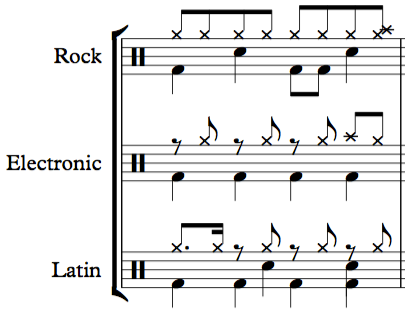
\includegraphics[width=0.6\textwidth]{ch03_symbolic/figures/patterns.png}
	\end{center}
	\caption[Rock, Electronic and Son-Based Pattern Used in Symbolic Listening Survey]{Rock, Electronic and Son-Based Pattern Used in Symbolic Listening Survey}
	\label{fig:symbolic_patterns}
\end{figure}

Three target patterns were used for the purposes of the test: a standard straight 8 rock pattern, a four-on-the-floor electronic pattern and a son-based latin pattern (\figref{fig:symbolic_patterns}). \tabref{tab:variable_summary} summarises all the variables under consideration for the evaluation. This resulted in a total of 72 \acrfull{wav} files with 3 fitness levels (inversely corresponding to the distance scores).

{\renewcommand{\arraystretch}{1.5}
\begin{table} 
	\begin{centering}
		\begin{tabular}{c c c c c}
\tabletop
Question & Measure & String & Pattern & Fitness\\	
\tablemid
Similarity & Hamming  & Linear & Rock & Low\\
Interesting & Swap & Parallel & Latin & Med\\
& & & Elec & High\\
\tablebot
		\end{tabular}
		\caption[Listener Survey Variable Summary]{Listener Survey Variable Summary}
		\label{tab:variable_summary}
	\par \end{centering}
\end{table}

Twenty-two participants took part in the survey, mostly drawn from music students and researchers. All of the participants confirmed that they played an instrument, 7 of whom specified a percussive instrument. Eighteen out of the 22 participants reported the ability to read music. It took approximately 15 minutes to complete.

\subsection{Results}

Before carrying out the statistical analysis the responses were summarised by computing the mode\footnote{Median or mode are generally considered more appropriate measures of central tendency when handling ordinal data such as Likert, and we use Spearman's Rho when performing correlation analysis for similar reason \citep{Boone2012, Lantz2013}.} of the Likert scores for each stimulus. Two “interestingness” stimuli out of the total 72 (36 for similarity, 36 for interestingness) were removed due to high divergence of opinion (50\% or more of the responses deviated by 2 or more Likert scale values from the mode).  

\figref{fig:like1} shows the overall fitness (normalised from its original range of [0-100] to the Likert range [1, 5]) against the mean and standard deviation of the Likert scores by each stimulus. The dip in the middle can be attributed to the different ranges of distance and corresponding fitness produced by the two string measures; the Hamming measure outputs values in a much higher and narrower range. This is more evident looking at the divided plots in \figref{fig:like2} , which plots fitness against Likert scores for each combination of string measure and representation type. 

\begin{figure}
\centering
\begin{subfigure}[b]{0.75\textwidth}
   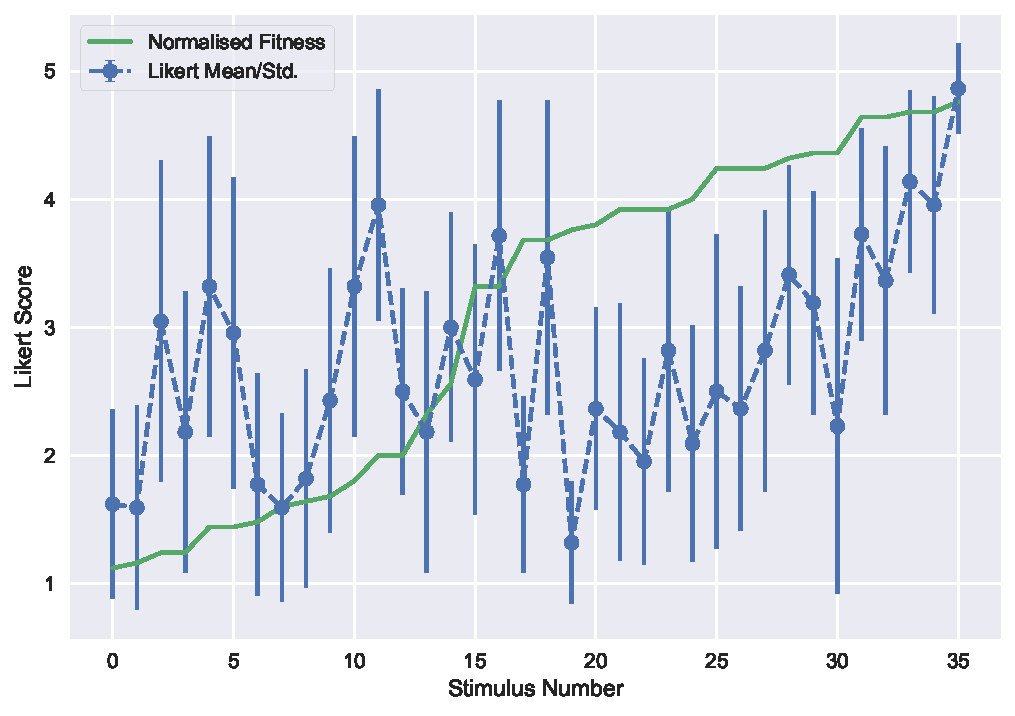
\includegraphics[width=1\linewidth]{ch03_symbolic/figures/total_likert.pdf}
   \caption{}
   \label{fig:like1} 
\end{subfigure}

\begin{subfigure}[b]{0.75\textwidth}
   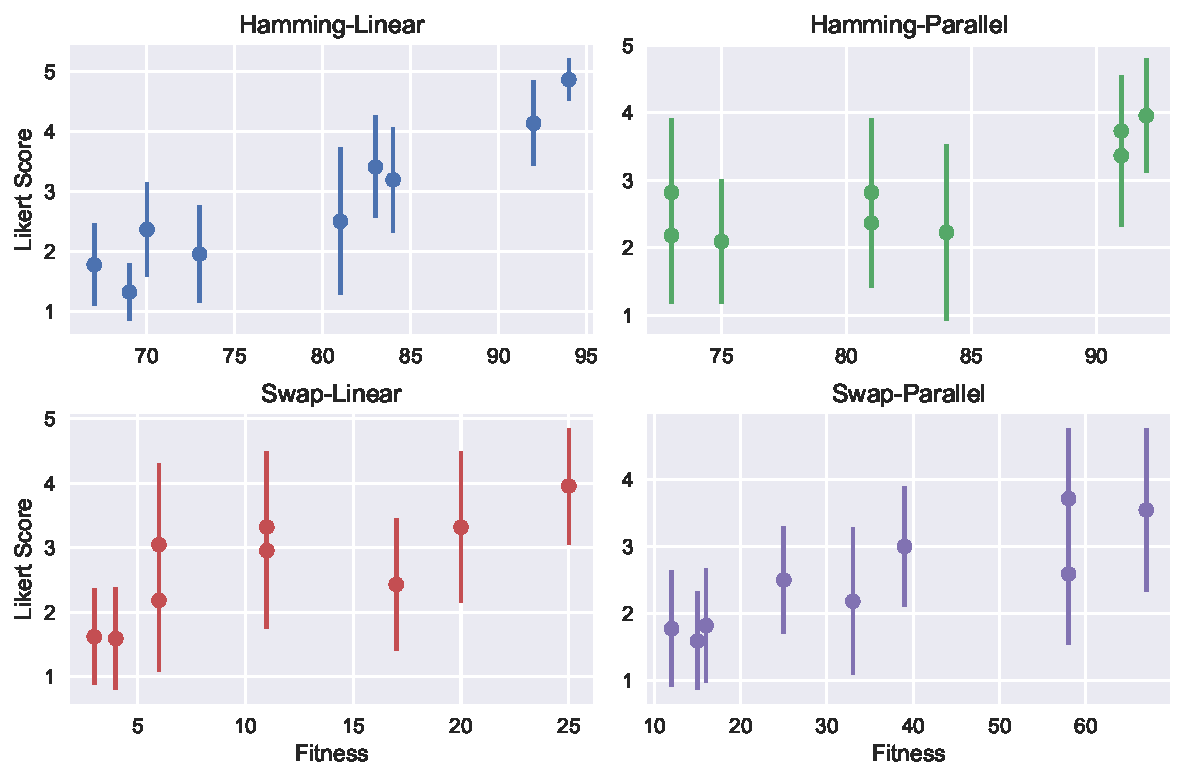
\includegraphics[width=1\linewidth]{ch03_symbolic/figures/separate_likerts.pdf}
   \caption{}
   \label{fig:like2}
\end{subfigure}

\caption[Mean and Standard Deviation of Fitness Versus Likert Scores]{Mean and standard deviation of fitness versus Likert scores for (a) each stimulus (b) measure and string type }
\end{figure}
\subsubsection{Similarity Ratings}

Our first task when looking at the data was to confirm whether inverse pattern distance and the fitness of the genetic algorithm correlates with the perceived similarity as determined by the participants. 

The data appears to suggest that this hypothesis is confirmed. \tabref{tab:overall_similarity_correlation} presents the Spearman ranked correlation matrix of fitness, distance and the mode scores received for each stimulus. There is a clear, strong negative correlation coefficient (\(\rho\) = -0.71, p < 0.05) between the distance measure and the perceived similarity to the target.  This correlation is not as clear with the fitness function, which can be attributed to the fact that fitness as a function of distance is evaluated differently for the two distance measures.

{\renewcommand{\arraystretch}{1.5}
\begin{table} 
	\begin{centering}
		\begin{tabular}{c | c c c}
\tabletop
& Distance & Fitness & Score\\	
\tablemid
Distance & 1.0000 & -0.4145 & -0.7134\\
Fitness & -0.4145 & 1.0000 & 0.4353\\
Score & -0.7134 & 0.4353 & 1.0000\\
\tablebot
		\end{tabular}
		\caption[Overall Similarity Correlation Matrix]{Overall Similarity Correlation Matrix}
		\label{tab:overall_similarity_correlation}
	\par \end{centering}
\end{table}

\figref{fig:hamming_versus_swap} shows the separated distance and fitness correlations against the mode scores for the Hamming and directed-swap distance measures. The fitness correlation values are 0.784 and 0.625 respectively and the distance correlation values are -0.784 and -0.716 respectively (p < 0.05). It can be seen that the Hamming distance has slightly better correlation.

\begin{figure}
	\begin{center}
		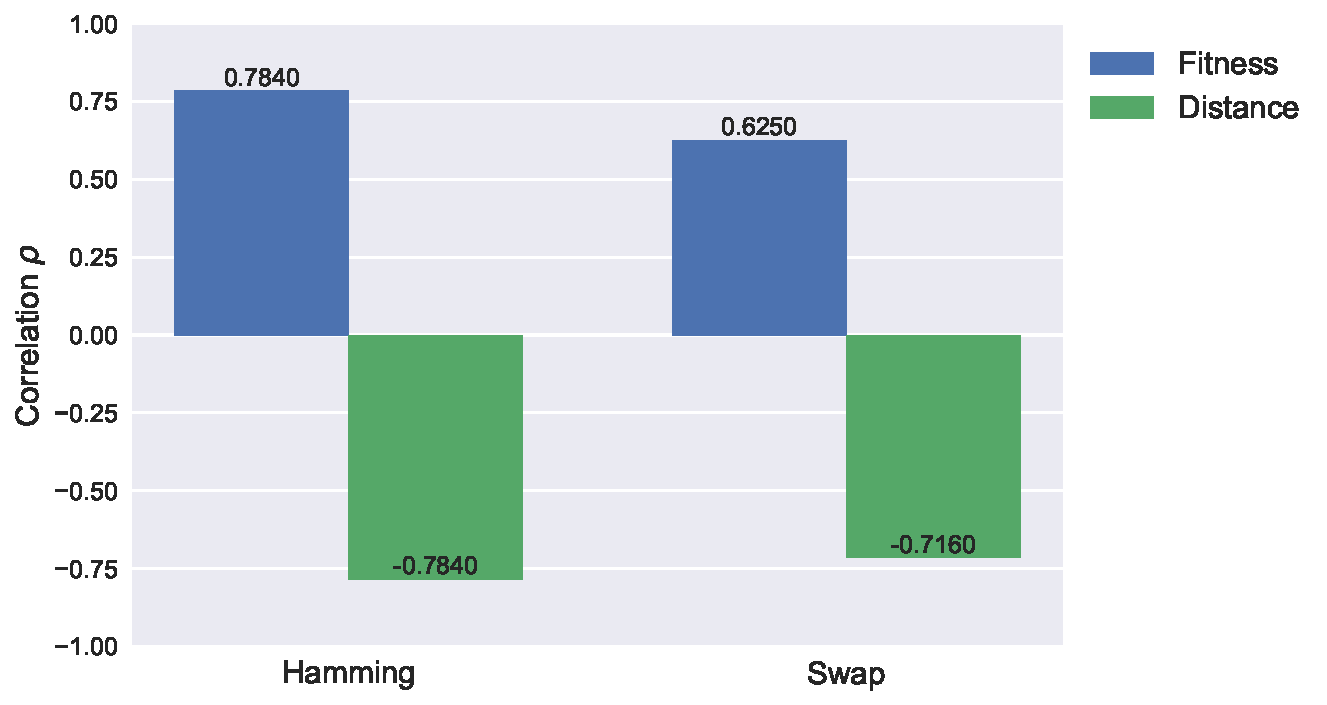
\includegraphics[width=0.75\textwidth]{ch03_symbolic/figures/measure_bar.pdf}
	\end{center}
	\caption[Fitness and Distance for Hamming and Swap Distance Metrics]{Fitness and Distance for Hamming and Swap Distance Metrics}
	\label{fig:hamming_versus_swap}
\end{figure}

\figref{fig:linear_versus_parallel} shows the separated distance and fitness correlations against the scores when we discriminate between linear and parallel pattern strings. The fitness correlation values are 0.525 and 0.480 respectively, and the distance correlation values are -0.852 and -0.576 respectively (p < 0.05). The linear representation scheme appears to correlate better with human judgement.

Post hoc analysis using a t-test and a Kruskal-Wallis non-parameteric \acrshort{anova} H-test compared the two different conditions - linear vs. parallel and hamming vs. directed-swap - and discovered a significant difference for the ratings of the distance measure (p < 0.05), but not in the case of the string representation type. Out of interest, we also examined the participants' musical experience in reading notation or playing a percussive instrument, but they had no significant effect on the ratings (p > 0.05) in both instances.

We can draw some tentative conclusions based on this data. Firstly, the strong correlation between the overall distance and similarity ratings suggest that, even for polyphonic string representations of drum patterns, distances such as the Hamming and directed-swap are useful measures of perceived similarity. Secondly, splitting and recombining the bit strings by timbre, as carried out in the parallel operation, does not seem to offer improvement over the simplistic, long bit string representation. Finally, the more complex directed-swap algorithm, with its ability to capture the ``horizontal'' displacement between two drum patterns, does not appear to reflect an increase in similarity scores in our survey, confirming Toussaint's finding but also extending it to the case of polyphonic patterns.

\begin{figure}
	\begin{center}
		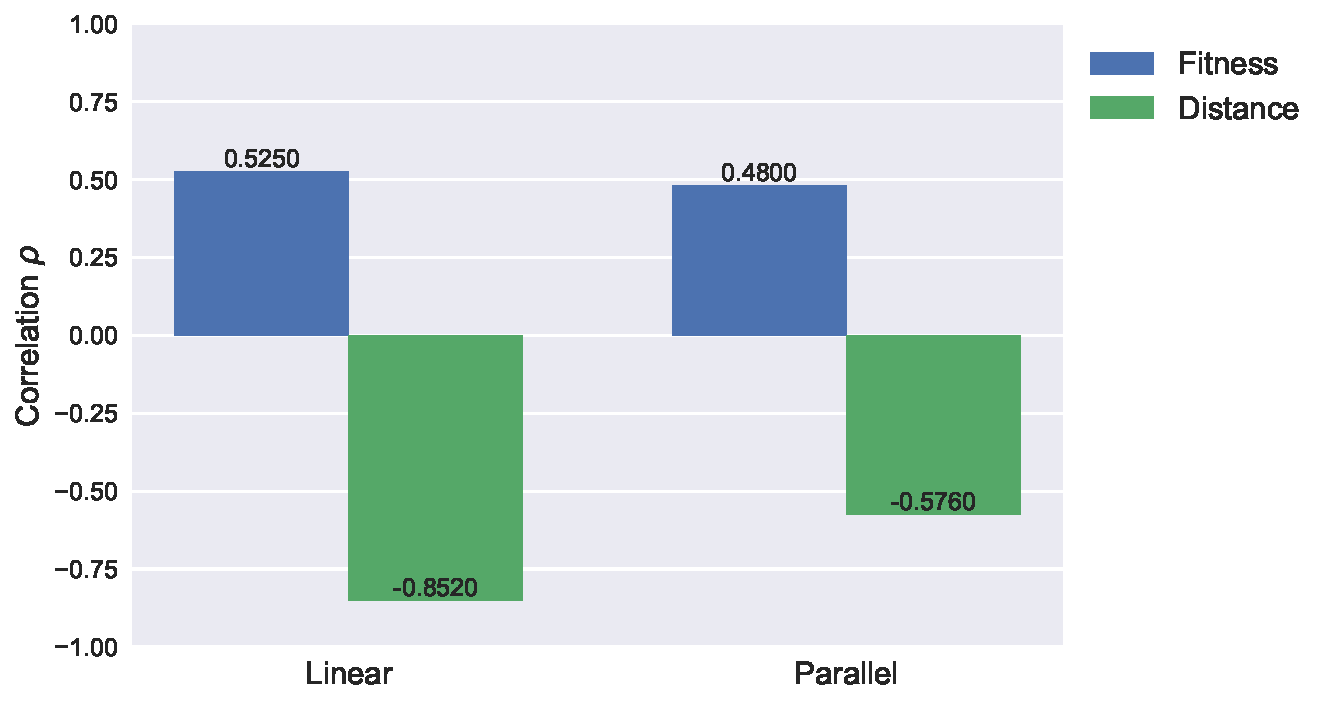
\includegraphics[width=0.75\textwidth]{ch03_symbolic/figures/reps_bar.pdf}
	\end{center}
	\caption[Fitness and Distance for Linear and Parallel String Computation]{Fitness and Distance for Linear and Parallel String Computation}
	\label{fig:linear_versus_parallel}
\end{figure}


\subsubsection{Subjective “Interestingness” Evaluation}

\tabref{tab:interestingness} presents the correlation matrix corresponding to the results of the users' impression regarding the "interestingness" of the patterns when heard in a sequence with the target. Curiously, the distance and fitness correlation coefficients are both positive, despite the fact that distance is inversely proportional to the fitness of the genetic algorithm but the p-values are so high (0.211 and 0.1887 respectively) that this data is not reliable. It is impossible to draw some meaningful or significant conclusions based on the disparity and inconsistency across subjects.

Disregarding the difficulty in appraising musically subjective output, the reason for this problematic data is largely attributable to the way in which we considered the notion of ``interestingness'' and how the question was formulated. Asking the participants to rate two essentially diametrically opposing qualities - i.e. variation (related to dissimilarity) and repetition (related to similarity) was a flawed approach that caused confusion. This became immediately apparent from some of the user feedback at the end of each survey session. For example:

\blockquote{\textit{“I noticed that I somehow prefer rhythms that are a natural
evolution of the previous pattern, instead of being totally different. But if the similarity with the previous pattern is too high, the result is still uninteresting to me, because the resulting pattern is too predictable and loses every appeal.”}}

To complete the survey then, users often reverted to their own rules to determine their ratings, as evident from these comments:

\blockquote{\textit{“Interestingness” was hard for me to evaluate. In the end I rated with a `good' interesting `bad' interesting system: if it's weird but i like it, it's in the first case, if not, in the second case.''}}

\blockquote{\textit{“.. There are some times on experiment 2 that the new rhythm might not be interesting for a complete section but that might be useful as a bridge or as a temporal loop marking the end of a section."}}

Another participant made the point that the pattern sequence may have forced some `expectation' regarding the concept of “interestingness”:

\blockquote{\textit{“... I have also the feeling that having the pattern repeated (ie AB twice), and therefore, having to come back to A again after having been in B, conditions very much the results.”}}

{\renewcommand{\arraystretch}{1.5}
\begin{table} 
	\begin{centering}
		\begin{tabular}{c | c c c}
\tabletop
& Distance & Fitness & Score\\	
\tablemid
Distance & 1.0000 & -0.5419 & 0.2201 \\
Fitness & -0.5419 & 1.0000 & 0.2310 \\
Score & 0.2201 & 0.2310 & 1.0000 \\
\tablebot
		\end{tabular}
		\caption[`Interestingness' Correlation Matrix]{`Interestingness' Correlation Matrix}
		\label{tab:interestingness}
	\par \end{centering}
\end{table}

Despite the apparent issues with our method of evaluation, the data and informal feedback does suggest that the genetic algorithm creates “interesting” musical output. Nineteen stimuli out of the 34 analysed registered a mode score value higher than 4 as seen by the 56\% green positive region in \figref{fig:interesting_distribution} (there were two responses for “Strongly Disagree”, but these were the two that were disregarded due to high divergence of opinion). The task ahead is to review the evaluation strategy in order to quantify and explain this aspect in a more coherent and predictable manner, decoupling the interdependency of the questioning between similarity and interdependence.

\subsection{Improving the System - Adding More Features}

\begin{figure}
	\begin{center}
		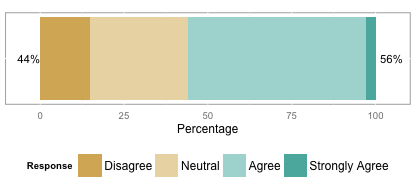
\includegraphics[width=0.85\textwidth]{ch03_symbolic/figures/interestingness.png}
	\end{center}
	\caption[Distribution of Responses for `Interestingness' in Symbolic Evaluation]{Distribution of Responses for `Interestingness'}
	\label{fig:interesting_distribution}
\end{figure}

The evaluation shows that our implemented methods do behave predictably in returning increasingly similar patterns to a target as the mean fitness of the genetic algorithm converges on its maximum. It also shows, despite deficiencies in the mode of questioning, that listeners do perceive these patterns favourably, given the sounds used and some localised awareness of style.

However we still felt that similarity methods alone were not capturing all of the subtleties inherent in symbolic rhythm patterns, features that other systems might include that prove more fruitful in analysis and generation. Another iteration of development on the genetic algorithm included three additional improvements that are described here.

\subsubsection{Timbre Weighting}

\label{sec:timbre_weighting}

Other than allowing the separation of the pattern into its constituent timbres for discrete generation in the parallel mode, our generative system makes no additional effort to extrapolate and delineate the obvious hierarchical and emergent roles the separate timbres induce in the sensation of drum patterns. 

Our brains process rhythm streams with different timbres and spectral profiles differently, and awareness and study of this fact goes some of the way to explaining why across different styles and cultures dispersion of timbres exhibit similar proportions across different frequency bands. To be precise we often see liberal placement of high-frequency, short attack timbres like hi-hats across all beats, while the kick drum usually enforces the downbeat\footnote{Let's forget about reggae for now!} and start of bar and finally the mid-range snare drums fills in the backbeat\footnote{Jazz and rock music attribute far greater importance to the backbeat though, which, much to the irritation of musicians, is not obvious to all concertgoers who insist on clapping on the `one and three' (\url{http://www.ethanhein.com/wp/2013/the-backbeat-a-literature-review/}). A very entertaining video shows a live concert where pianist Harry Connick Jr. uses rhythmic displacement to insert a bar of 5/4 in a 4/4 piece of music. This intentionally shifts the clapping audience from `one and three' to the `two and four' backbeat, much to the relief and gratitude of the drummer! (\url{https://www.youtube.com/watch?v=--qv9SI6vws)}}. As \cite{Merchant2015} observes in the general scope of pop music 

\blockcquote[]{Merchant2015}{``\textit{...the vast majority of drum patterns in popular music have bass drum hits on the downbeat (e.g. beats 1 and 3 of a 4/4 pattern) and snare hits on the upbeats (beats 2 and 4). While not inviolable, this statistical generalization leads listeners familiar with these genres to have strong expectations about how to assign musical events to a particular metrical position, thus using learned top-down cognitive processes to reduce the inherent ambiguity of the musical surface.}''}

Other researchers also point to the salience of the kick and snare drums in the inference of downbeats and upbeats in rhythm perception and, consequently, its computational analysis \citep{Zils2002, Panteli2014a, Gomez-Marin2017}. Leaving aside \textit{why} exactly this is the case \footnote{\cite{Hove2014} proposes that ``its our superior time perception for lower musical pitch''.}, it is clear that not all drum timbres are created equal, and generative systems such as ours should incorporate some cognisance of that important fact.

To remedy this, a weighting scheme was used to assign different degrees of importance to the separate timbre streams when operating in parallel mode. The exact formulation weights are not important, just that they are weighted sufficiently to bias the fitness function as desired, so for example we weigh the 4 streams successively from bottom (kick) to top (perc or cymbal) with  the set $W = \{2, 1, 0.5, 0.25\}$. These weights are also parametric to account for different timbres assigned to the different streams.

\subsubsection{Syncopation}

\blockcquote[]{Toussaint2013}{``\textit{Syncopation is the spice of rhythm}''}

Just as musical ideas blossom through the balance between repetition and variation of a motif or loop, rhythms are made infinitely interesting by resolving the tension arising from anticipation and reinforcement of the beat and the deliberate disruption of that expectation. The \textit{Harvard Dictionary of Music} defines syncopation simply as:

\blockcquote[]{Apel1969}{``\textit{Syncopation: a momentary contradiction of the prevailing meter or pulse}''}

\cite{Gomez2005} expand on this definition:

\blockquote{\textit{``Moreover, syncopation can be materialized either as a momentary change of the primary character of the meter or as a contradiction between strong and weak beats against other parts of the musical texture whose metrical context is fixed''}}

Up until now, our algorithm has only been considering the similarity of generated rhythms in relation to the target, and has no facility to gauge the level of syncopation present in the target or the generated rhythms. It would be a useful parameter of the \acrshort{ga} to allow the user to increase bias for selecting candidates based on relative syncopation of strong and weak beats in a particular track, and this was the next feature that was implemented.

\cite{Eigenfeldt2013} incorporate a rudimental quantifier for level of syncopation into their hybrid rhythm algorithm by simply counting the number of onsets that do not fall on the expected strong beats in the metre (4/4).

To expand our system to include knowledge of syncopation, we turned once again to perceptual literature to see if there were any established analytic methods that prove more grounded in observation rather than blindly devising our own. \cite{Gomez2005} sum up 4 such measures including:

  \begin{figure}
	\begin{center}
		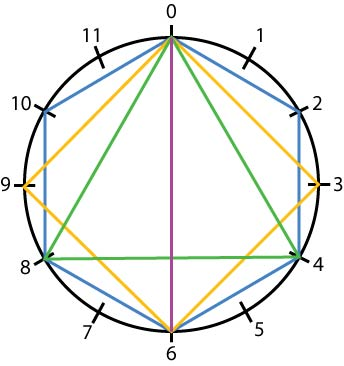
\includegraphics[width=0.3\textwidth]{ch03_symbolic/figures/offBeatness.jpg}
	\end{center}
	\caption[Toussaint's Off-Beatness Measure]{Toussaint's Off-beatness measure. (Image from McGill).}
	\label{fig:offbeatness}
	\end{figure}
	
\begin{itemize}
  \item The Rhythmic Oddity Property \citep{arom2004african} is not really a measure, it is simply a boolean value indicating whether there exists two onsets in a pattern that divide the set equally or not.
  \item Toussaint's \textit{Off-Beatness} \citep{Toussaint2004African} finds those geometric shapes that divides an $N$ length rhythm necklace evenly (\figref{fig:offbeatness}). These are the on-beats. The number of onsets that lie outside of these geometric entities give the degree of off-beatness.
  \item Keith's Measure \citep{keith1991polychords} defines syncopation in terms of three events, \textit{hesitation} (a note starts on a beat but ends off a beat), \textit{anticipation} (a note starts off a beat but ends on a beat) and \textit{syncopation} as a combination of of hesitation and anticipation within a rhythm. Weights are assigned to these three event categories (like our own timbre weightings used in \secref{sec:timbre_weighting}, these are subjective by the author) and the weighted sum of instances of these constitute the measure of syncopation in the measure.
\end{itemize}}

\cite{Gomez2005} criticises Keith's measure in its arbitrary assignment of weights but, more crucially, its restriction to binary metres (explained in depth the article). They offer a new measure to address these limitations and coalesce some elements inherent in Toussaint's off-beatness. The key tenet of the \acrfull{wnbd} is that ``notes are supposed to end where the next note starts''. Onsets that land off strong beats are given the smaller weighting and weighting increases to a maximum as notes cross over strong beats - which they posit gives the strongest sensation of syncopation. 

\blockcquote[]{Gomez2007}{\textit{``the closer a note is to a strong beat, the more syncopated it sounds; and second, the syncopation effect is stronger when a note crosses over only one strong beat of the meter.''}}

While \cite{Song2013} has some reservations of this model and we could find no instances of surveys that evaluated its correlation with human listeners, it does seem a reasonable distillation of syncopation for our purposes, compared to the other formulations.  \acrshort{wnbd} is distance-based model that can be easily integrated into our fitness function with comparative ease.  Based on a reference implementation offered in Synpy \citep{Song2015}, a Python environment for syncopation modelling, we expanded the genetic algorithm to include the \acrshort{wnbd} in its fitness function.

\subsubsection{Density}

The density of a rhythm is an easy feature to comprehend, \cite{Wiggins2012a} defines it as the ``mean number of events per tactus beat''. We simply added another metric for the fitness function to consider, given by the average number of onsets per pattern (\eqnref{eq:density}), where $x_i$ is onset number $i$ and $N$ is the total number of onsets.

\begin{equation}
\label{eq:density}
	d(x)=\frac{\sum_{i=1}^{N}x_i}{N} \quad \text{if}\ x_i=1
\end{equation}

\begin{figure}
	\begin{center}
		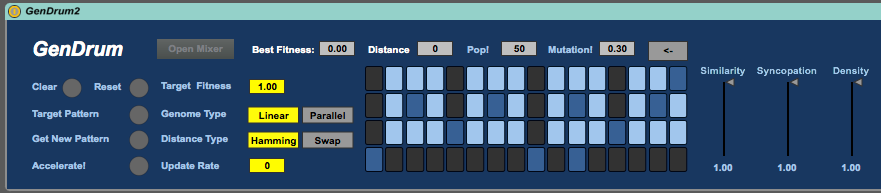
\includegraphics[width=1.0\textwidth]{ch03_symbolic/figures/gendrum2.png}
	\end{center}
	\caption[GenDrum with Expanded Feature Parameter Control]{GenDrum with expanded feature parameter control to the right.}
	\label{fig:gendrum2}
\end{figure}

Having influence over density in a generative drum machine is a desirable control to have and  has actually been shown to be a useful descriptor in modelling rhythmic similarity, specifically in dance music signals \citep{Panteli2014a}. Within the GiantSteps project the Agnostic Density Transformer \citep{Jorda2016} is a generative drumming system that is focussed on density control of individual drum sounds based on corpus analysis, and has since been expanded into a mobile app by Reactable Systems\footnote{\url{https://reactable.com/snap/}}.

The weighted linear combination of these three features coupled with the new parallel timbre weighting scheme comprise the new fitness function for the genetic algorithm. Since these additional features represent a considerable departure from the general string analytics offered by the SimpleGA object, we decided to encapsulate it in a separate, specialised object called RhythmGA. \figref{fig:gendrum2} shows the revised interface for GenDrum that uses the new \acrshort{ga}, along with the new similarity, syncopation and density  sliders that adjust the relevant parametric weights.

\subsection{Conclusions and Closing Remarks}

In this chapter we presented a way of generating drum patterns automatically using genetic algorithms. Rather than relying on the commonly used interactive fitness function, our method was shown to use the notion of a “target pattern”, with fitness derived from the distance of the generated patterns to the target. This was devised to address the way dance music composers derive tracks from a bottom-up approach that begins with a small loop or idea that is iteratively expanded through repetition and variation of its key features.

Following a review of various approaches to establishing the distance between rhythms as present in the literature, we demonstrated the implementation and incorporation of two such measures - the Hamming distance and the directed-swap distance - into a genetic algorithm instrument for polyphonic drum pattern creation. We believe this work, and the accompanying articles, constitute the first integration of perceptual symbolic similarity research in rhythmic pattern generation with genetic algorithms.

To evaluate the research carried out, we conducted a listening survey to determine participants' reaction to the generated patterns in terms of the similarity and “interestingness” related to the target pattern. It was shown that the distance ,and thus fitness, correlates strongly with user perception in terms of similarity. Crucially we showed that the Hamming distance alone is a worthwhile quantifier of rhythmic similarity even in the case of polyphonic patterns. Our approach to gauging users' response to the concept of  “interestingness”, however, needs review and presents a complex challenge for future work. 

Based on the feedback ascertained during the evaluation, a second iteration of the genetic algorithm along with the accompanying instrument was developed that assimilated an expanded feature set as well as enhanced parametric control for the user. By adjusting these parameters, relative weightings of rhythmic attributes such as similarity, syncopation and densities can bias the fitness function as appropriate. While our own informal appraisal of these additions was favourable, a more rigorous evaluation and listening survey was not conducted. This was due to a shift of focus away from symbolic algorithm composition towards approaches involving content-based, \acrshort{mir}-driven synthesis of real audio.

The reasons for this change of tack were multifold. Firstly, while genetic algorithms coupled with an appropriately formulated fitness function demonstrably provide a legitimate mechanism for generating rhythms for dance music, methods proposed by our colleagues that invoke specialised metrics \citep{Marin2015} or knowledge trained on large corpora representing style \citep{Jorda2016} are perhaps more suited. This has been confirmed in a collaborative evaluation conducted by ourselves along with others in the GiantSteps consortium \citep{Vogl2016}. Our \acrshort{ga} did not fare better in various listening tests against neural networks and a database-driven method both trained on human derived patterns from the Maschine software and hardware environment (and understandably so, as the two methods indisputably embed more knowledge). However it did return more ``interesting'' results and was rated higher in its facility for creating more unique fill patterns. 

%Article dealing with Listener Surveys from MuMe
%
%Agres, K., Forth, J., \& Wiggins, G. A. (2016). Evaluation of musical creativity and musical metacreation systems. Computers in Entertainment, 14(3), 1–33. https://doi.org/10.1145/2967506

But most of all, based on an overall critique of the myriad approaches to generating rhythms using symbolic conventions and similarity analysis (including our own experiences building systems that utilise them), we sensed that there are some subtleties inherent in real recordings and performances of rhythms that are not encapsulated via these means. Namely we could identify:

\begin{itemize}
\item The notion of verticality or interdependence between concurrent elements at discrete points in time that are not completely captured by concepts such as metrical hierarchy and weighting.
\item Stress and accents that affect the dynamics of onsets in a pattern, not captured by the pervasion of binary representations that exists in literature and associated realised systems. This perhaps can be addressed by analysing and estimating rhythms in terms of real or floating point numerical forms.
\item Related to stress and accents there are other difficult phenomena of human factors in music that include groove and swing. These are notoriously difficult facets to define and quantify by musicologists, and even harder to estimate and recreate using computational means. The need to replicate human qualities of time within conventional music production systems is clear however. Most \acrshort{daw}s at least include some ability to adjust metrical positioning of note information according to some percentage factor ostensibly tantamount to groove.
\item The timbral qualities - or the sounds and processing used to derive the patterns - we contend have a profound impact on the perceptual response and aesthetic impression of the loop. Simply assembling rhythms according to perceptual similarity measures using arbitrary sounds (all too frequently coarse \acrshort{midi} approximations) does not always produce the desired results, at least in generative attempts at dance music.
\end{itemize}

All these factors were carefully considered and it became more apparent that perhaps the symbolic domain was not sufficient for our goals. The focus of the thesis turns to investigating whether these methods can be refined, adapted and extended to systems that generate rhythms using signals and thus connecting time with timbre.or 
\cleartorecto%!TEX root = ../thesis_a4.tex
\chapter{State of the Art in Sampling-Based Composition}
\label{chap:sota}

\blockquote{``\textit{It's not where you take things from, it's where you take them to}''}

\begin{flushright}
(Jean-Luc Godard)
\end{flushright}

\blockquote{\textit{``Rip it up and start again.''\footnote{Also the title of another Simon Reynolds book on music culture, this time charting the rise of postpunk from 1978-1984 \citep{reynolds2009rip}}}}

\begin{flushright}
(Edwyn Collins with Orange Juice)
\end{flushright}

As we move away from the symbolic leanings of the previous chapter and head towards audio content-based approaches to music generation, we pause once again from the deeper technical discourse to establish some context, both artistic and historic, before before providing a thorough definition of a concatenative synthesis - a form of synthesis that is rooted deeply in audio sampling - and its key works from the literature and community.

I use the term ``audio content-based'' here interchangeably here with sampling for good reason. The term actually stems from \acrshort{mir} parlance, used to dermarcate research that deals  directly with audio data and signals from those that analyse notated information and metadata \citep{Veltkamp2008, Casey2008a}. It also enforces the idea that we are working with elements extracted from found and realised objects and artefacts, which we will soon discover has a long and illustrious history as a creative aesthetic.  

\section{Artistic Context}

Historically, reusing existing material for the purposes of creating new works has been a widely practised technique in all branches of creative arts. The manifestations of these expressions can be wholly original and compelling or otherwise derivative, uninspiring and potentially copyright infringing depending on myriad factors, including the domain of the work, the scale of the reuse, and its cultural context.

In the visual arts, reusing or adapting existing material is most immediately understood in the use of collage, where existing works or parts thereof are assembled to create new artworks. Cubist artists such as George Braque and Pablo Picasso extensively referenced, appropriated and reinterpreted their own works and the works of others (\figref{fig:picasso}), as well as common found objects from their surroundings \citep{Greenberg1971}. Collage would later serve as direct inspiration for bricolage, reflecting wider postmodernist trends towards deconstructionism, self-referentiality,  and revisionism that include the practice of parody and pastiche \citep{Lochhead2002}. 

\begin{figure}
	\begin{center}
		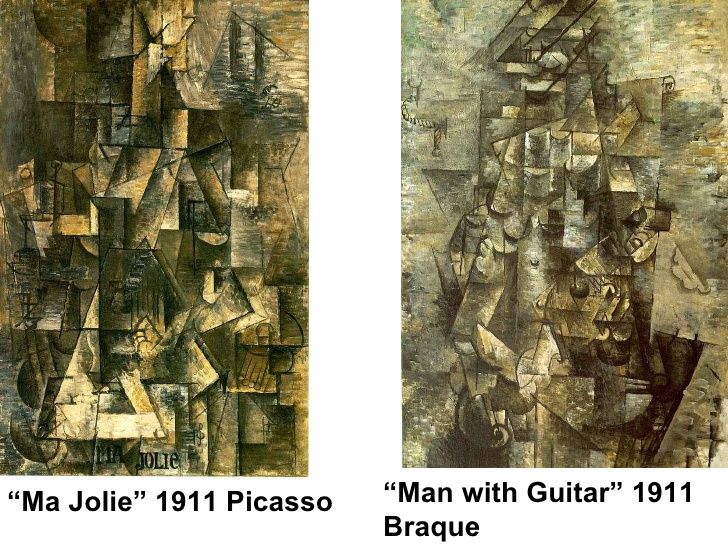
\includegraphics[width=0.9\textwidth]{ch04_sota/figures/picasso.png}
	\end{center}
	\caption[Cross-Referential Cubist Works by Picasso and Braque]{Cross-referential Cubist works by Picasso and Braque.}
	\label{fig:picasso}
\end{figure}
\subsection{Musique Concrète and Elektronische Musik}

In music and the sonic arts, its natural corollary came in the form of musique concrète \citep{Holmes2008}, a movement of composition stemming from the experiments of Pierre Schaeffer and, later, Pierre Henry at the studios of Radiodiffusion-Télévision Française in Paris during 1940s and 1950s \citep{Battier2007a}. In contrast to the artificially and electronically generated \textit{elektronische musik} spearheaded by Karlheinz Stockhausen at the \acrshort{wdr} in Cologne \citep{Collins2011a, Bates2009}, the French composers sought to conceive their works from existing recorded sound, including environmental sources like trains and speech. Seemingly unrelated and non-musical sounds were organised in such a way that the listener discovered the latent musical qualities and structure they inherently carry.

It is important to note that, in music composition, general appropriation of work predates these electronic advancements of technology. In Western art music, for example, composers like Bela Bartók – himself a musicologist - have often turned to folk music for its melodies and dance music styles \citep{Bartok1993}, while others such as Debussy \citep{Tamagawa1988} became enchanted by music from other cultures such as Javanese Gamelan, studying its form and incorporating the ideas into new pieces. Quotations, or direct lifting of melodies from other composers’ works, frequently crossing into classical, are also quite common, and has become a frequent, and often with the intention of being amusing, rudiment in jazz music practice \citep{Mangani2006}\footnote{\cite{Appel2002} recounts an anecdote of Stravinsky attending a Charlie Parker gig at his residency in the Birdland club in New York and ``[roaring] with delight, pounding his glass on the table'' on hearing a snippet of the opening of his Firebird Suite from the saxophone of the bebop pioneer.}.  For more on appropriation and quotation music a good reference is compiled by \cite{Metzer2003}.

\subsection{Granular Synthesis of Microsound}

Granular synthesis is composition at the microscale of sound - or to use Curtis Roads' term \textit{microsound} \citep{Roads2004}. It is a molecular viewpoint of music that \cite{Thomson2004} maintains finally promises the composer the possibility for ``total composition'', thereby dictating the parameters of everything from higher-order forms and structures all the way down to infinitesimal sonic minutiae.

It is generally agreed that the physicist Dennis Gabor first proposed the first quantum theory of sound that suggested ``large, complex sound events are composed of simple acoustic particles, or sonic grains' \citep{Miranda1995}. This was later reiterated and expanded on by Xenakis in \textit{Formalized Music} \citep{Bradshaw1973}, who laboriously arranged small snippets of tape material to produce \textit{Analogique B} (for 9 string instruments and tape, 1959) \citep{Robindore2009}.

Curtis Roads lays claim to developing the first digital implementation of granular synthesis \citep{Roads1998}, during the latter half of the 1970s (on punchcards!) and has composed with it and written about it capaciously ever since \citep{Roads1985, Roads1991, Roads1996, Roads2004} Barry Truax successfully achieved real-time granular synthesis during the 1980s with the composition of \textit{Riverrun} \citep{Truax1998}, using Poisson distributions and tendency masks to control the limits of typical granular parameters like frequency range, grain duration, modulation index, and delay.

Practically speaking, granular synthesis is, as \cite{Roads1998} suggests, a type of additive synthesis. Rather than mixing pure signals generated by oscillators to generate complex sounds, small `grains' (within the realm of 20-200ms) of existing sounds\footnote{Though these grains can, and often do, come from signal generators.} are superimposed to create dense amalgamations or `clouds' of sound grains \citep{Collins2011a, Thomson2004}. Nowadays granular synthesis is widespread in computer music practice and most music programming environments like Pd, Max and Reaktor, and even commercial synthesisers and \acrshort{daw}s,  provide extensive tools and tutorials for its pursuit. Listening to the works of glitch artists like Kim Cascone\footnote{The ideals of which are put forth in his influential manifesto ``The aesthetics of failure: ``Post-digital'' tendencies in contemporary computer music'', the most cited article in The Computer Music Journal \citep{Cascone2000}}\citep{Latartara2010}, or the more meditative washes of sound from drone and noise luminaries Tim Hecker or Fennesz, reveals an instantly recognisable application of the technique. 

I have used granular synthesis (\figref{fig:wolfcastle}) frequently in my own music for generating large indeterminate textural material from smaller fragments of composed musical ideas or interesting samples I have stumbled on. Recently this included a work  for violin, distortion and granular synthesis presented as part of the concert programme\footnote{Incidentally, Barry Truax premiered a new work during the same conference} of the \acrfull{smc} conference\footnote{\url{http://www.maynoothuniversity.ie/smc15/concert2.html}} as well as a quadrophonic soundscape that was installed at the Sonic Environments/\acrfull{acmc} satellite event that took place as part of \acrfull{nime} in 2016\footnote{\url{http://www.sonicenvironments.org/program.html}}. 

\begin{figure}
	\begin{center}
		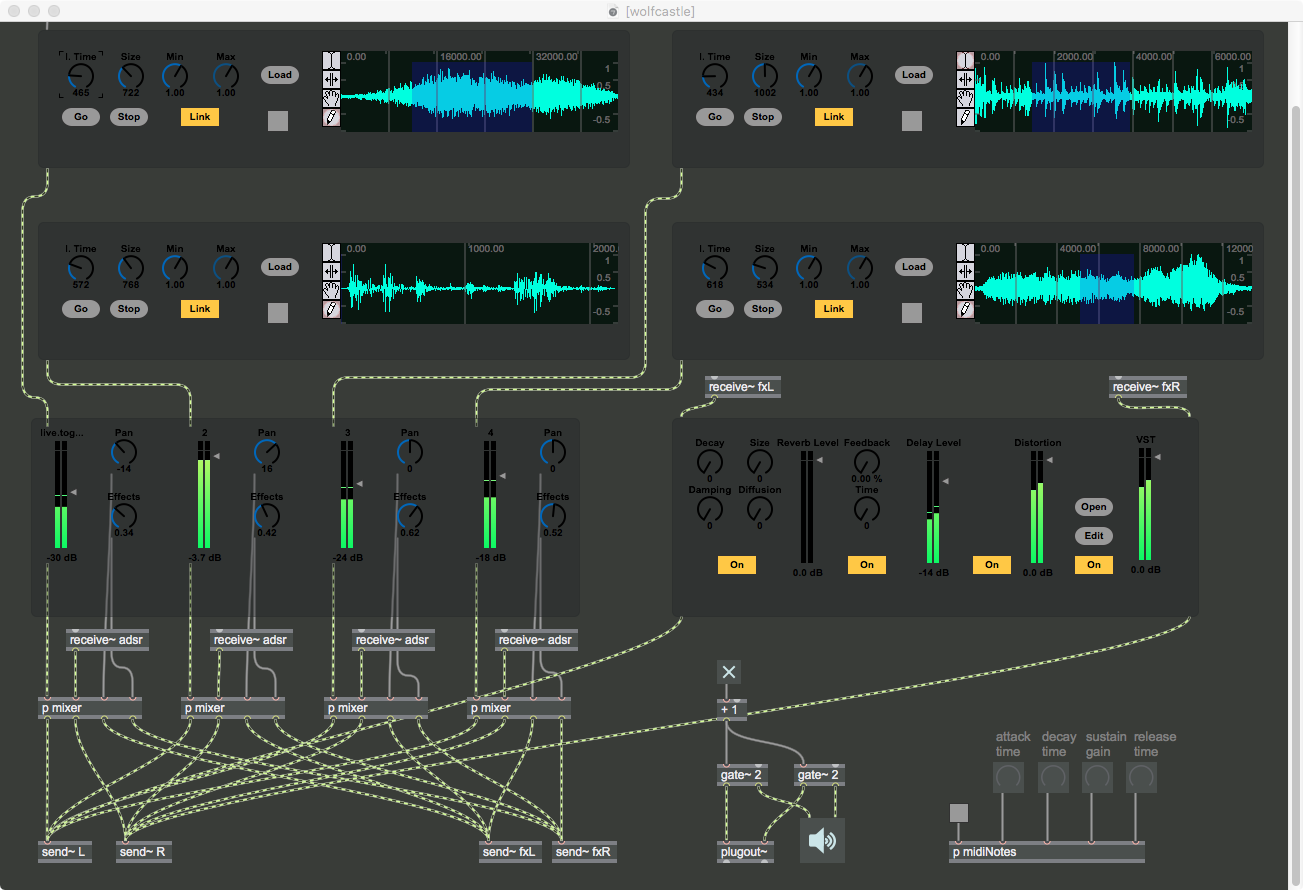
\includegraphics[width=1.0\textwidth]{ch04_sota/figures/wolfecastle.png}
	\end{center}
	\caption[Screenshot of My Four-Channel Granular Synthesiser for Max]{Screenshot of my four-channel granular synthesiser for Max\footnote{\url{https://github.com/carthach/Wolfcastle}}}
	\label{fig:wolfcastle}
\end{figure}

\subsection{Bring the Noise - Hip Hop Culture and the Birth of the Breakbeat}

In \chapref{chap:dancemusic} we briefly highlighted the contribution of DJ Kool Herc, who used two turntables to produce an extended looping, collage of drum sections (the breakbeats) from identical vinyl records \citep{Forman2004}. Kool Herc's contemporaries, Afrika Bambaataa and Grandmaster Flash observed his discovery and augmented it with more rudiments such as backspin, punch phrasing and, of course, record scratching which would widen the idiomatic vocabulary of \textit{turntablism} within the burgeoning subculture of hip-hop \citep{Smith2000}.

Vinyl would not reign king for too long however. The modern notion of sampling, at least in non-electroacoustic or contemporary composition circles, stems from the advent of the digital sampler and its eventual explosion of adaptation in hip-hop. The arrival of easy to use, self-contained hardware systems like the Akai \acrfull{mpc} offered the rhythmic sequencing facilities of the Roland TR range but with the groundbreaking ability to import one's own sounds (or more crucially, other artists' sounds), and all this with a reasonable price tag attached \citep{Rodgers2003}.

Hip-hop producers quickly latched onto the possibilities of these new tools. Artists such as Public Enemy and Beastie Boys, on albums like \textit{It Takes a Nation of Millions to Hold Us Back} and \textit{Paul's Boutique} respectively, painstakingly assembled bewildering permutations of musical samples, soundbites and miscellaneous other recorded materials that sought to supplant the many cultural references that permeated their lyrics \citep{Sewell2013, Sewell2014}. 

As was also identified in \chapref{chap:dancemusic}, the influence of hip-hop production would later inform the sample-heavy arrangements of jungle and drum and bass, in particular with its exhaustive re-rendering of the infamous ``Amen Break'' and James Brown's ``Funky Drummer''. In fact these breaks had already been dissected previously in hip-hop, long before UK producers got their digital surgical scalpels to them. The Amen Break appears on NWA's landmark gangster rap album \textit{Straight Outta Compton} and James Brown's ``Funky Drummer'' shows up on tracks by Run DMC and LL Cool J \citep{Frane2017}, leading \cite{Oliver2015} to observe that ``it is [Funky Drummer] sampled and recontextualized so extensively as to achieve near ubiquity in a wide range of popular music genres''.

Jungle and drum `n' bass was dealt with sufficiently in \chapref{chap:dancemusic} so it is hopefully not necessary to restate its relevance and impact on sample-based composition here. It is prudent to point out though that, since we are edging towards computational models and processes that automate audio content-based composition, that there is already a strong body of work that specifically addresses computational aspects of breakbeat analysis and its sequent generative synthesis. Nick Collins for example, has dedicated much of his academic dissemination to algorithms that can replicate the distinctive stuttering and glitching tropes that pervade in jungle, drum \& bass and post jungle emergent styles like breakcore \citep{Collins2001, Collins2002, Collins2006a}. Hockman has also devoted significant output to \acrshort{mir}-oriented analysis of timbral and rhythmic aspects unique to these styles \citep{Hockman2007, Hockman2012, Hockman2015}.

\subsection{Plunderphonics and Metamusic}

\blockquote{``\textit{I quote from others the better to express myself}''}

\begin{flushright}
(Michel de Montaigne)
\end{flushright}

I think it's rather appropriate that the quote above I did not discover myself, instead I lifted it from an article dealing with the appropriation and quotation of other works in music \citep{Holm-Hudson1997}. The article is mostly concerned with the implications arising from the work of John Oswald, an artist who has gained much notoriety in his career by directly challenging musical copyright law for artistic gain. As hip-hop producers were trailblazing a new sound through intimate operation of the digital sampler, the inevitable direction was the bootlegging of other artists' music for creative repurposing, thus sparking the huge copyright debate. Record companies and legal representatives struggled to react to the huge paradigm shift in cultural production whose commercialisation was no longer under their total jurisdiction. The ethics of all this are outside the scope of this thesis obviously, but at least a few legal commentators at the time recognised that perhaps the long established laws governing creative ownership were no longer fit for purpose:

\blockcquote[]{Arewa1979}{``\textit{...copyright doctrine incorporates notions of Romantic authorship that assume independent and autonomous authorship and even genius in the creation of original musical works. This individualistic and autonomous vision of musical authorship, which is central to copyright law, has deemphasized the importance and continuity of musical borrowing practices generally}''}

Returning to John Oswald, who, capitalising on the polemics and its scope for creative interpretation, coined the name ``plunderphonics'' and set out his artistic intentions in a suitably subtitled 1985\footnote{Interesting then, that around this time Truax and Roads were still getting to grips with granular synthesis.} essay "Plunderphonics, or Audio Piracy as a Compositional Prerogative” \citep{Oswald1985}. The Canadian composer and media artist, inspired by the Dadaist cut-up literary technique practised by beat writer William S. Burroughs as well as sound collages by James Tenney \citep{Cox2004}, began to use tape-splicing techniques to create deliberately recognisable montages of other musical recordings, particularly pop music such as Michael Jackson or Led Zeppelin. If granular synthesis represents, as \cite{Thomson2004} indeed suggests,  a path to ``total composition'', then Oswald's modus operandi for composition is, as \cite{Holm-Hudson1997} describes it, the ``total importation'' of pieces involving ``reinterpretation or rehearing of existing recordings'' \citep{Cutler1994}.

Nowadays artists such as Girltalk and DJ Danger Mouse\footnote{Danger Mouse availed of the tendency in rap music to realise acapella versions of records for the purposes of remixing to create \textit{The Grey Album}: a well-received mashup of The Beatles' \textit{White Album} with Jay Z's \textit{The Black Album} \citep{Gunderson204}}\footnote{And much prior to that, experimental ensemble Negativland faced the legal backlash of record labels when they released the EP \textit{U2}, which contained misleading artwork and unauthorised sampling of the rock group, but ironically catapulted them into public notoriety \citep{herman1998politics, lysloff2003music}.} create extremely complex and multi-referential intersections of popular music harnessing the powerful beat matching and synchronisation capabilities of the modern \acrshort{daw} \citep{Humphrey2013}. The style has become known widely as ``mashups'' or ``bastard pop'' \citep{McGranahan2010} and straddles the fine line of what constitutes and can be protected under the auspices of fair usage \citep{Mongillo2009}, the very same doctrine that allows us to include images from other sources in this thesis in good faith.

Many computational works have emerged that explicitly mention and address the musical goals of mashup \citep{Tokui2008, Davies2013, Davies2014a, Davies2014b, Lee2015, Smith2015, Meroo-Peuela2017}, and we shall see that the direct consequence of concatenative synthesis can facilitate the realisation of elements of mashup.

\section{Concatenative Synthesis}

Recent associated research efforts in computer music, signal processing and music information retrieval afford us the opportunity to develop automated and intelligent systems that apply the aforementioned aesthetic of sampling and artistic reuse. 

The term ``concatenative synthesis'' (or musical mosaicing \citep{Zils2001}) has been extensively used to describe musical systems that create sound by recycling existing ones automatically, according to some well-defined set of criteria and algorithmic procedures \citep{Schwarz2000}. Concatenative synthesis can be considered the natural heir or big brother to granular synthesis. With concatenative synthesis, the grains of sound become “units” and are more related to musical scales of length, such as notes and phrases. Most importantly, descriptive information is attached to these units of sound: crucial features that allow the temporal, spectral, harmonic and timbral characteristics of the sound to determine the sequencing of final output. 

The criteria governing the procedure of concatenative synthesis is usually applied in relation to some reference sound or target that the composer wishes to emulate, and with this in mind, Bernardes gives a more thorough definition of the discipline:

\blockcquote[]{Bernardes2013}{``\textit{[Concatenative Synthesis] is a technique for synthesizing sounds by concatenating short audio segments (called units). It relies on a large database of segmented and descriptor-analyzed sound snippets (called corpus) to assemble a given target phrase by selecting the units that best match the target specification according to a distance measure in the descriptors}''}

In \chapref{chap:symbolic} we described symbolic methods that could take a seed or target rhythm pattern typical of dance music and replicate and variate it through similarity knowledge embedded in the fitness function of a \acrshort{ga}. With concatenative synthesis, we have a computational framework that can extend this notion of looping repetition and variation to audio. 

Just as granular synthesis invokes Heisenberg's Uncertainty Principle to blur the lines of time and frequency at the microscale of sound \citep{Truax2005}, we can view concatenative synthesis as a macroscale manipulation of the dichotomy between originality and theft determined by the scale of the unit - larger units of scale are more fully-formed but are more likely to be recognised as being lifted from other sources, while smaller units eventually approach granular levels of abstraction.
\section{Survey of Concatenative Synthesis Systems}

Other authors have previously provided insightful summaries of research trends in concatenative synthesis. In particular we suggest those by \cite{Schwarz2005, Schwarz2006b} and \cite{Sturm2006}. These surveys are over 10 years old however, so we offer here a more recent compendium of state of the art systems as we see them, based on our investigations of previous publications up until now.

\subsection{Unit Selection Synthesis of Speech}

Before music, concatenative synthesis has enjoyed successful application in the area of speech processing, specifically in the synthesis of \acrfull{tts}.

\cite{Hunt1996} were the first to propose unit selection synthesis using \acrfull{hmm}s as a means for combining phoneme units extracted from existing audio recordings of speech. \cite{Conkie1999} remarks that ``for unit selection synthesis, typically phone-based, it is possible to produce sentences that sound surprisingly natural and intelligible from a large database'. Since then many researchers \citep{Conkie1999, balestri1999choose, schroder2001emotional, Tihelka2010, Lakkavalli2010} and software systems \citep{black1994chatr, beutnagel1999t, Young2002} have cemented the popularity of the technique.

We will treat unit selection and \acrshort{hmm}s more thoroughly in \chapref{chap:pyconcat} but essentially \acrshort{hmm}s extend Markov chains (\secref{sec:markov_chains}) by assuming that the states in the state machine are now hidden but can output observable symbols. The Viterbi algorithm can return the most probable sequence of hidden states given a particular sequence of observed symbols. In concatenative synthesis, this maximum probabilistic model is inverted to facilitate minimal cost computations thereby encoding the dissimilarity of unit sounds.

Formulating the problem in terms of a \acrshort{hmm} enables us to capture two important contributors to a successful synthesis via the \textit{target cost} and the \textit{concatenation cost} (\figref{fig:target_concat_costs}). The target cost estimates the penalty of matching a corpus unit with the current target unit based on a target specification that stipulates factors like fundamental frequency or pitch, duration, position in the syllable and surrounding context of phonemes. The concatenation cost then estimates the quality of the join between two potential corpus units if they were to be selected, hence allowing a means of penalising selections that introduce unwanted jumps in energy and pitch (for example) that could lead to an unnatural sound. The Viterbi algorithm efficiently searches the state space of database units and outputs indices corresponding to the optimal state sequence for the target, based on a consolidated linear combination of the aforementioned costs \citep{Ob1995, Hunt1996}.

\begin{figure}
	\begin{center}
		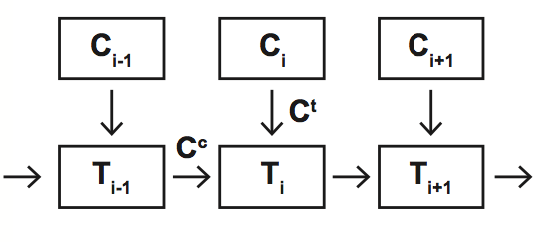
\includegraphics[width=0.6\textwidth]{ch04_sota/figures/costs.png}
	\end{center}
	\caption[Target and Concatenation Costs in a Text-To-Speech HMM Compared]{Target ($C^{t}$) and concatenation ($C^{c}$) costs in a \acrshort{tts} \acrshort{hmm} compared.}
	\label{fig:target_concat_costs}
\end{figure}

\subsection{Musical Concatenative Synthesis}
\label{sec:zilsone}
 
Schwarz directly applied Hunt’s HMM approach for musical purposes in his Caterpillar \citep{Schwarz2003}. He notes, however, that the HMM approach can be quite rigid for musical purposes since it produces one single optimised sequence without the ability to manipulate the individual units. To address these limitations, he reformulates the task into a constraint satisfaction problem which offers more flexibilities for interaction. A constraint satisfaction problem models a problem as a set of variables, values and a set of constraints that allows us to identify which combinations of variables and values are violations of those constraints, thus allowing us to quickly reduce large portions of the search space \citep{Russell2002}. 



Constraint satisfaction for concatenative synthesis was first introduced previously by \cite{Zils2001}, in what they describe as musical mosaicking or, to use their portmanteau, musaicing. They define two categories of constraints: segment constraints and sequence constraints. Segment constraints control aspects of individual units (much like the target cost in a \acrshort{hmm}-like system) based on their descriptor values. Sequence constraints apply globally, and affect aspects of time, continuity and overall distributions of units. The constraints can be applied manually by the user, or learned by modelling a target. The musically tailored “Adaptive Search” algorithm performs a heuristic search to minimise the total global cost generated by the constraint problem. One immediate advantage of this approach over the HMM is the ability to run the algorithm several times to generate alternative sequences, whereas the Viterbi process always outputs the most optimal solution.

 A simpler approach is presented in MatConcat \citep{Sturm2004}, using feature vectors comprising six descriptors and computing similarity metrics between target units and corpus units. Built for the Matlab scientific computing environment, the interface is quite involved, and the user has control over minute features such as descriptor tolerance ranges, relative descriptor weightings as well as window types and hop sizes of output transformations. On his website are short compositions generated by the author using excerpts from a Mahler symphony as a target, and resynthesised using various unrelated sound sets, for instance pop vocals, found sounds and solo instrumental recordings from saxophone and trumpet.

As concatenative synthesis methods matured, user modalities of interaction and control became more elaborate and real-time operations were introduced. One of the most compelling features of many concatenative systems is the concept of the interactive timbre space. With the release of CataRT \citep{Schwarz2006} the authors provided an interface (\figref{fig:catart}) that arranges the units in an interactive two-dimensional timbre space. The arrangement of these units is made according to a user-selectable descriptor on each axis. Instead of using a target sound file to inform the concatenation procedure, the user’s mouse cursor becomes the target. Sounds that are within a certain range of the mouse cursor are sequenced according to some triggering options (e.g. one-shot or  looped) and, most crucially, with real-time output.

\begin{figure}
\centering
\begin{subfigure}[b]{0.9\textwidth}
   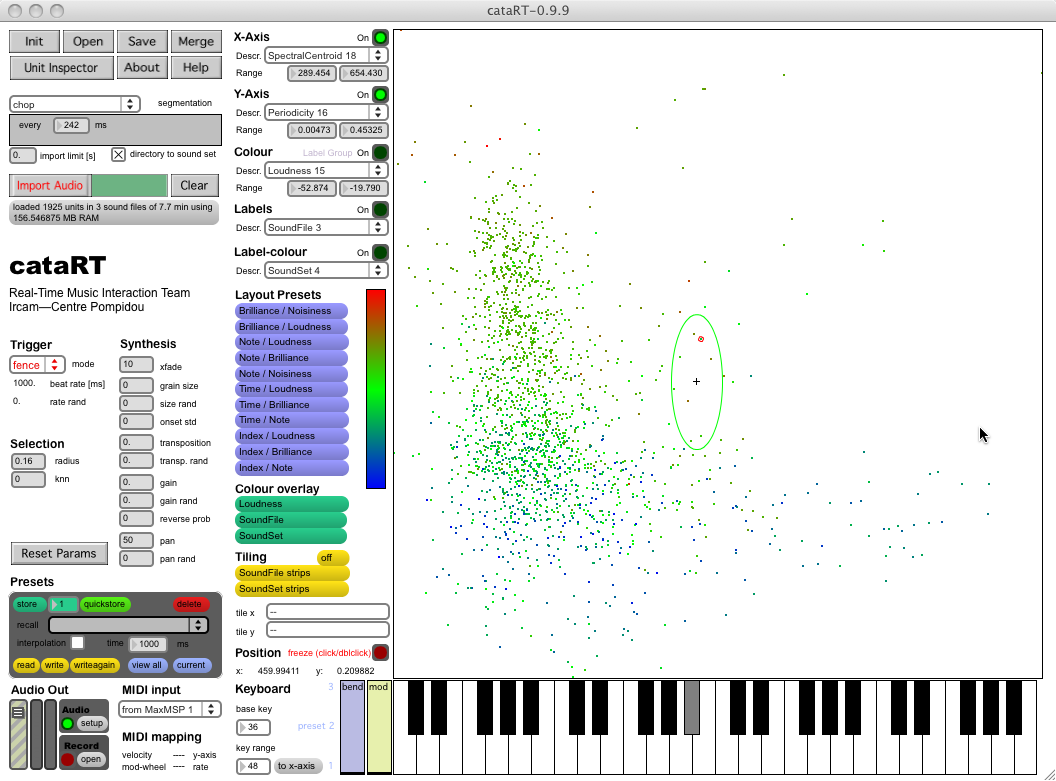
\includegraphics[width=1\linewidth]{ch04_sota/figures/catart.png}
   \caption{}
   \label{fig:catart} 
\end{subfigure}

\begin{subfigure}[b]{0.9\textwidth}
   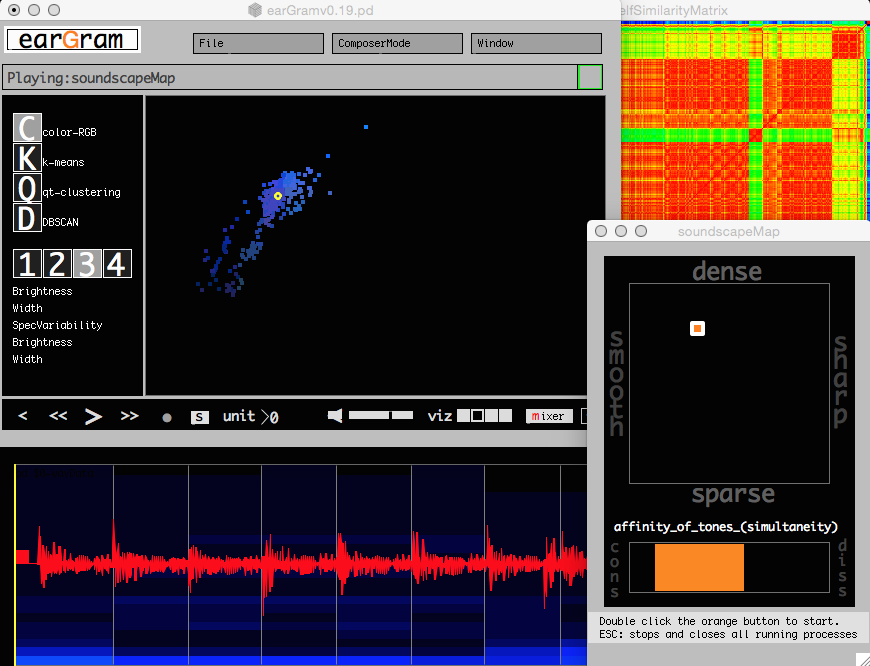
\includegraphics[width=1\linewidth]{ch04_sota/figures/eargram.png}
   \caption{}
   \label{fig:eargram}
\end{subfigure}

\caption[CataRT and Eargram Interfaces]{(a) CataRT \acrshort{gui} (Image from IRCAM), (b) earGram User Interface (Image from  SMC INESCTEC), both showing a clear realisation of an explorable 2D timbre space.}
\end{figure}

Bernardes takes inspiration from CataRT and also from Tristan Jehan’s Skeleton \citep{Jehan2005} to build his EarGram system for the Pure Data environment \citep{Bernardes2013}. Built on top of William Brent’s excellent feature extraction library timbreID \citep{Brent2010}, it adds a host of interesting features for visualisation and classification.  For instance, as well as the familiar waveform representation and previously described 2D timbre representation (\figref{fig:eargram}) (with various clustering modes and dimensionality reduction implementations), there are similarity matrices that show the temporal relations in the corpus over time. Some unique playback and sequencing modes also exist, such as the infiniteMode, which generates endless playback of sequences, and the soundscapeMap, which features an additional 2D control of parameters pertaining to sound scene design. Another system that adapts a 2D timbre space is Christian Frisson’s AudioGarden \citep{Frisson2010}, which offers two unique mapping procedures. The first of which, “Disc” mode, places units by assigning the length of the audio file to the radius of the unit from the centre, with the angle of rotation corresponding to a principal component of timbre (\acrshort{mfcc}s).  In the other Flower mode, a point of the sound is positioned in the space according to the average \acrshort{mfcc} coefficients of the entire sound file. Segments of the particular sound are arranged in chronological fashion around this centre point.

\begin{figure}
\centering
\begin{subfigure}[b]{0.9\textwidth}
   \includegraphics[width=1\linewidth]{ch04_sota/figures/audiogarden.png}
   \caption{}
   \label{fig:Ng1} 
\end{subfigure}

\begin{subfigure}[b]{0.9\textwidth}
   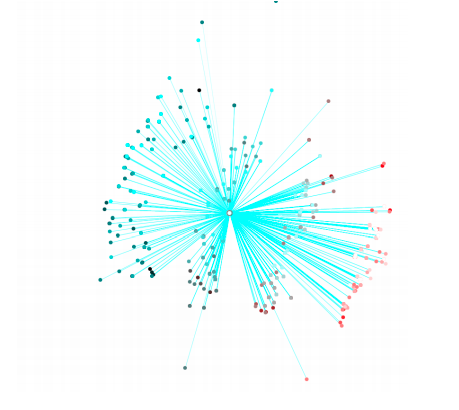
\includegraphics[width=1\linewidth]{ch04_sota/figures/audioguide.png}
   \caption{}
   \label{fig:audioguide}
\end{subfigure}

\caption[AudioGarden and AudioGuide Interfaces]{Two different visualisation of timbre: (a) AudioGarden ``Disc'' Visualisation (Image from \cite{Frisson2010}), (b) AudioGuide Clustering Visualisation around Target (Image from \cite{Schwarz2012}).}
\end{figure}

There have been some concatenative systems tailored specifically with rhythmic purposes in mind. Xiang proposes Granuloop \citep{Xiang2002} for automatically rearranging segments of 4 different drum loops into a 32 step sequence. Segmentation is done manually, without the aid of an automatic onset detector, using the Recycle sample editing software. Segmented sounds are compared using the inner product of the normalised frequency spectrum, supplemented with the weighted energy. These values become weights for a Markov-style probability transition matrix. Implemented in Pd, the user interacts by moving a joystick, in a 2D space, this then affects the overall probability weightings determining which loop segments are chosen. The system presents an interesting approach but is let down by its lack of online analysis. Ringomatic \citep{Aucouturier2005} is a real-time agent specifically tailored for combining drum tracks, expanding on many of the constraint-based ideas from their prior musaicing experiments. They applied the system to real-time performance following symbolic feature data extracted from a human \acrshort{midi} keyboard player. They cite, as an example, that a predominance of lower register notes in the keyboard performance applies an inverse constraint that creates complementary contrast by specifying that high-frequency heavy cymbal sounds should be concatenated.

As demonstrated in EarGram, concatenative synthesis has been considered useful in sound design tasks, allowing the sound designer to build rich and complex textures and environments that can be transformed in many ways both temporally and timbrally. Also in connection to sound design, \cite{Cardle2003} report on their Directed Sound Synthesis software as a means of providing sound designers and multimedia producers a method of automatically reusing and synthesising sound scenes in video. Users select one or more regions of an existing audio track, and can draw probability curves on the timeline to influence resynthesis of these regions (one curve per region) elsewhere. Soundscapes by \cite{Hoskinson2001}, in a nod to granular synthesis, refers to their segments as ”natural grains” and seek to synthesise endless streams of soundscapes. The selection scheme by which segments are chosen is based on a representation of each segment as a transition state in a Markov chain. Its interface features knobs and sliders for interactively controlling gain and parameters of multiple samples. To evaluate the platform they conducted an additional study \citep{Hoskinson2007} to reveal whether listening subjects found the concatenated sequences convincing compared to genuinely recorded soundscapes.

More specific and applied use cases of concatenative synthesis include \cite{Hackbarth2010}, who works intimately with the possibilities of concatenative synthesis in large scale music composition. He has worked with Schwarz to provide an alternative interface for exploring variations based on a force-directed graph (\figref{fig:audioguide}) to give a visual impression of the perceptual distances units in relation to a central target, not unlike the feedback we provided in our GenDrum instrument (see \chapref{chap:symbolic}). O’Connell describes a graphical system for Pd that demonstrates the use of higher level perceptual concepts like mood (happy vs sad) for informing selection in audio mosaics \citep{OConnell2011}.

Commercial implementations also exist for concatenative synthesis. Of particular note is Loopmash\footnote{\url{https://www.steinberg.net/en/products/mobile_apps/loopmash.html}}, a software plugin and mobile application for automatically creating mashups from existing looped content. The interface consists of a number of tracks in a timeline arrangement. One track is set as a master, and slices in the master are replaced with matching slices from the other slave tracks. Users interact by manipulating “similarity gain” sliders that control the influence of each track in the slice selection algorithm. Other applications exist more as \acrshort{midi} sampler systems attempting to model the performance qualities of natural sources such as orchestral ensembles\footnote{\url{https://www.synful.com/}} or the human voice\footnote{\url{https://www.vocaloid.com/en}}.

There are many other concatenative systems that are too numerous to discuss in detail here. \tabref{tab:concat_system_summary} compiles a summary of all the systems we came across in our research, with remarks on interaction and visualisation features, support for rhythm, and whether any user evaluation was carried out.

\subsection{Future Directions - Mixing and Source Separation}

Most concatenative synthesis systems we have studied (including those techniques we propose) tend to consider the concatenation process in purely horizontal and temporally inclined terms.  Naturally, it is pertinent to question whether the same process can be accomplished systematically in the vertical dimension characterised by the frequency spectrum. Or, in more simpler terms - can we stack units on top of each other systematically in addition to chaining them in sequence? While not the focus of this thesis (but certainly a promising avenue for further study), we briefly summarise relevant topics of interest and  techniques that are or can be used.

\subsubsection{Vertical Selection with Mixture Models}

\cite{Hoffman2009} have outlined a system that seeks to recreate the target \textit{spectrum} by, as Coleman describes it \citeyearpar{Coleman2010}, \textit{superimposing} (using convolution) a series of spectra from a corpus. To reduce the complexity associated with high dimensionality, a search space reduction with a \acrfull{mcmc} is applied. 

In a version of AudioGuide by Hackbarth \citep{Hackbarth2013}, they also outline the system's facility for enabling ``layered sounds'' and ``vertically stratified complexes'' based on formulas \citep{Tardieu2008}  developed for a prior system in the OpenMusic environment called Orchidée or Automatic Orchestration Tool \citep{Carpentier2010}. The goal of their work is to transfer some of the principles of traditional orchestration (combining and arranging for instruments to create desired blends of timbre) to the realm of computer music by allowing prediction of mixtures as well as concatenations to match a target specification of a sound.

Hackbarth \citep{Hackbarth2010} describes the derived ``Subtractive Spectral Algorithm'' for superimposition. When an appropriate unit is selected from the corpus as a candidate match for the target, its time-varying Mel-amplitudes are subtracted from  the target sound and a `residual' target spectrum remains. The unit selection procedure is performed repeatedly until it halts when the residual target spectrum energy falls below a certain threshold. The resulting units are then mixed together additively. A visual depiction of this over several mixtures can be seen in \figref{fig:spectrum_subtraction}. Clearly the algorithm tends towards selection of louder units initially, with gradually softer ones emerging as the subtracted target energy diminishes. 

\cite{Coleman2015} invokes the term ``mixtures'' to describe concatenative synthesis problems where the corpus might not have all the features to effectively simulate a target, but a carefully selected combination of them might. He uses the analogy of several single notes combining to form a chord, except the synthesis engine would use a weighted combination of superimposed frames mixed together.

\begin{figure}
	\begin{center}
		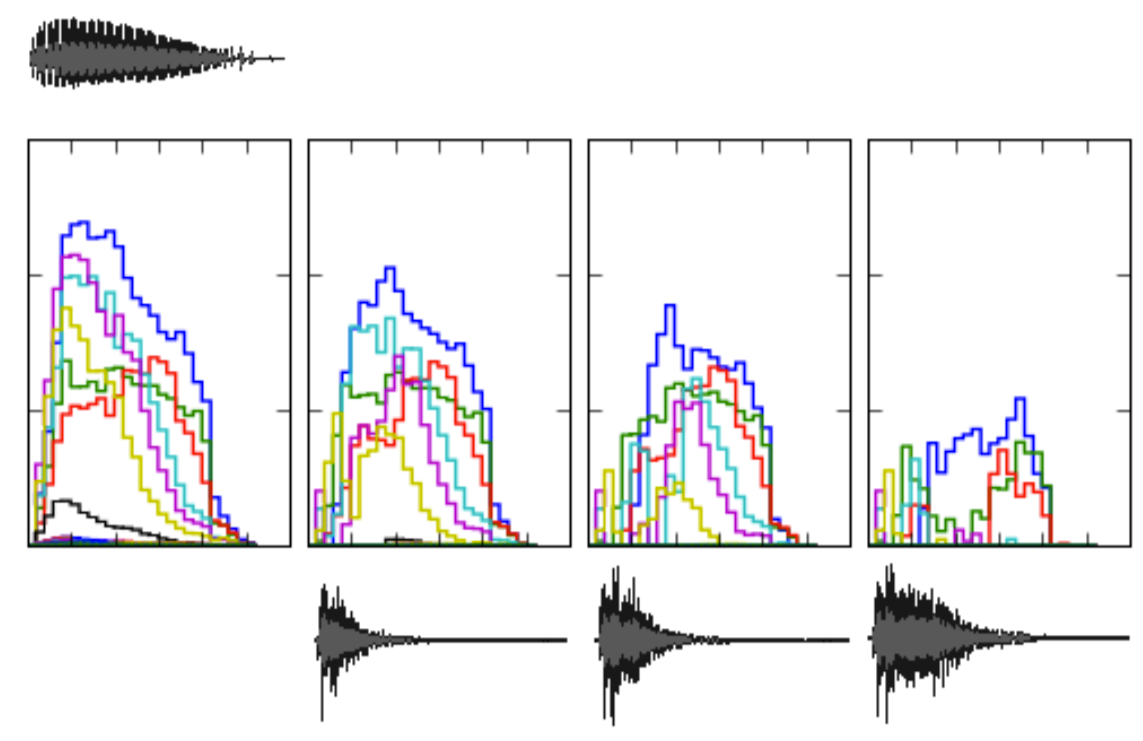
\includegraphics[width=0.75\textwidth]{ch05_pyconcat/figures/spectrum_subtraction}
	\end{center}
	\caption[Spectral Subtraction Algorithm in AudioGuide]{Visual depiction of spectral subtraction algorithm in AudioGuide. Image from \cite{Hackbarth2010}.}
	\label{fig:spectrum_subtraction}
\end{figure} 

\subsubsection{Vertical Segmentation with Source Separation}

We shall note in \secref{sec:yin}, in the case of the missing fundamental frequency, our auditory system is remarkable in its processing ability and inference engine. More remarkably,  perhaps, is its innate capacity for on the fly separation of real-time audio signals at will, or to give it its technical term, blind source separation. In pyschoacoustic auditory scene analysis research \citep{Bregman1994}, source separation is illustrated usually in terms of the ``Cocktail Party Effect'': how is a human, at a social event, able to separate voices from background noise and home in on particular conversations? In musical source separation this is even more elusive - consider picking out individual instruments in an orchestral passage, especially when, as \cite{Miron2017a} stresses, sources are likely to be correlated in time and frequency. Computational auditory scene analysis seeks to replicate this extraordinary human processing ability through digital signal processing means \citep{Wang2006}.

Initial efforts in computational source separation often involved matrix decomposition methods such as non-negative matrix factorisation, as demonstrated in the work of 
\cite{Fitz2004}. Fitzgerald's initial focus was on automatic drum transcription via source separation but later gained wider recognition with some some successful demixing and upmixing from mono to stereo of recovered archive Beach Boys recordings \citep{Fitz2004}. More recent state of the art approaches are once again successfully exploiting deep learning methods trained on large sets of musical data in genres like Western classical \citep{Miron2017a, Miron2017}.

Just as a concatenative synthesis system will use onset detection to split larger sound files into smaller units along the time domain, source separation opens up the possibility of theoretically segmenting complex sounds in the frequency domain according to instrument, or more accurately, \textit{streams} that hopefully contain related instruments (all depending of course on the material to be separated and the models upon which the system has been trained).

We envisage this as particularly useful in concatenative synthesis of drum rhythms. Perhaps a producer might want to decompose a number of kits into their constituent parts and mix and match with sounds from other sources. Mixing electronic drum sounds generated by a drum machine with naturally recorded acoustic drum sounds is a common strategy in dance music and source separation could prove invaluable here.


\newpage
\thispagestyle{empty}
\mbox{}

\begin{sidewaystable}
	\begin{threeparttable} 
		\ra{1.0}
%		\small
		\begin{centering}
			\begin{tabular}{l l l l l}
				\tabletop
				Author (Year) & Name & Evaluation & Interface & Rhythm or Tempo\\
				\tablemid			
				\cite{Schwarz2000}                & Caterpillar                   & No                     & 2D explorer                  & No             \\
				\cite{Zils2001}         & Musaicing                     & No                     & ?                            & Yes            \\
				Hazel(2001)               & Soundmosaic                   & No                     & Command Line                 & No             \\
				\cite{Hoskinson2001}      & Soundscapes                   & No                     & Waveform/Menus               & No             \\
				\cite{Xiang2002}          & Granuloop                     & No                     & 2D Controller                & Yes            \\
				\cite{Kobayashi}          & Sound Clustering Synthesis    & No                     & ?                            & No             \\
				\cite{Cardle2003}         & Directed Soundtrack Synthesis & Videos of use cases    & Waveform/Menus               & No             \\
				\cite{Lazier2003}         & MoSievius                     & No                     & ?                            & Looping        \\
				\cite{Sturm2004}          & MATConcat                     & No                     & Waveform/Menus               & No             \\
				\cite{Lindemann2007}		& Synful (Commercial)           & Not available          & Knobs/Sliders                & No             \\
				Casey (2005)                  & Soundspotter                  & Retrieval Accuracy     & Native Pure Data             & No             \\
				\cite{Aucouturier2005} & Ringomatic                    & User Experiment        & Lists/Menus                  & Drumming Tool  \\
				\cite{Simon2005}          & Audio Analogies               & Algorithm Performance  & None                         & No             \\
				\cite{Jehan2005}                  & Skeleton                      & Algorithmic evaluation & Waveform/Menus               &                \\
				\cite{Schwarz2006}                & CataRT                        & No                     & Timbre Space              & Looping option \\
			    Weiss et al. (2009)           & None                          & No                     & Waveform Segments            & No             \\
				\cite{Frisson2010}         & AudioGarden                   & No                     & Timbre Space / Waveform   & No             \\
				\cite{Hackbarth2010}			& AudioGuide                    & No                     & 2D CataRT based              & No             \\
				\cite{OConnell2011}             & None                          & Yes                    & Native Pure Data             & Looping demo   \\
				\cite{Bernardes2013}            & EarGram                       & Author's impressions   & Timbre Space and Matrices & Looping			\\	
				\tablebot		
			\end{tabular}
			\par \end{centering}		
		\begin{tablenotes}
			\small
%			\item[] ABBREVIATIONS: NA=Not applicable; GD=Group Delay, PDE=Probability Density Estimate
		\end{tablenotes}
			\caption[Summary of Existing Concatenative Sound Synthesis Systems]{Summary of existing concatenative sound synthesis systems}
			\label{tab:concat_system_summary}
	\end{threeparttable}
\end{sidewaystable}
 
\cleartorecto%!TEX root = ../thesis_a4.tex
\chapter{Specifying and Exploring Concatenative Synthesis}
\label{chap:pyconcat}

\section{Introduction}

As we discovered in \chapref{chap:sota} there exists a bewildering number of systems that propose or apply some level of concatenative synthesis technique. However widespread these methods are, some commonality arises across the majority of these when they are examined in closer inspection. Some of the important stages that we identify across this landscape include: 

\begin{enumerate}
  \item \textit{Unit Decomposition} - Automatically segmenting larger sound files into constituent units using musically and perceptually relevant criteria.
  \item \textit{Feature Extraction} - Selecting and applying meaningful combinations of multi-level music descriptors than can be utilised to summarise and compare units of sound effectively.
  \item \textit{Unit Selection} - Combining units of sound according to some criteria, commonly using some notion of a \textit{target} to compare constituent features against.  
\end{enumerate}

This chapter explores in depth these key facets. We describe the most common algorithms and techniques used in the literature and offer improvements where we see fit. In practical terms, all of the research carried out is implemented and encapsulated within a framework for Python we call \textit{PyConcat}, described in more detail in Appendix  \ref{app:pyconcat}. 

\section{Unit Decomposition}

Musical signals and sounds convey meaningful information at hierarchical levels of temporal scale. Choosing which level to work with naturally depends on the goals of the composer in tandem with the musical context. \figref{fig:beltram} visually depicts the different levels of scale that we can work with in concatenative synthesis tasks, beginning with the low-level framewise snippets in either the time or frequency domains. Framewise units are most typically used in granular synthesis but combined with feature analysis they are also found in many concatenative systems. Larger units can naturally be extracted uniformly (at regular time intervals), but the most common unit timescale used in concatenative system is as a result of performing some class of onset detection procedure. Onset detection algorithms are used to automatically detect events in audio signals. With an appropriately implemented algorithm and careful adjustment of its parameters based on the program material, the idealised output provides a list of time indices that correspond to the placement of a musical note. At the highest level of scale, we can use more involved and complex feature analysis to extrapolate units based on beat tracking and/or estimated tempo for example.  

\begin{figure}
	\begin{center}
		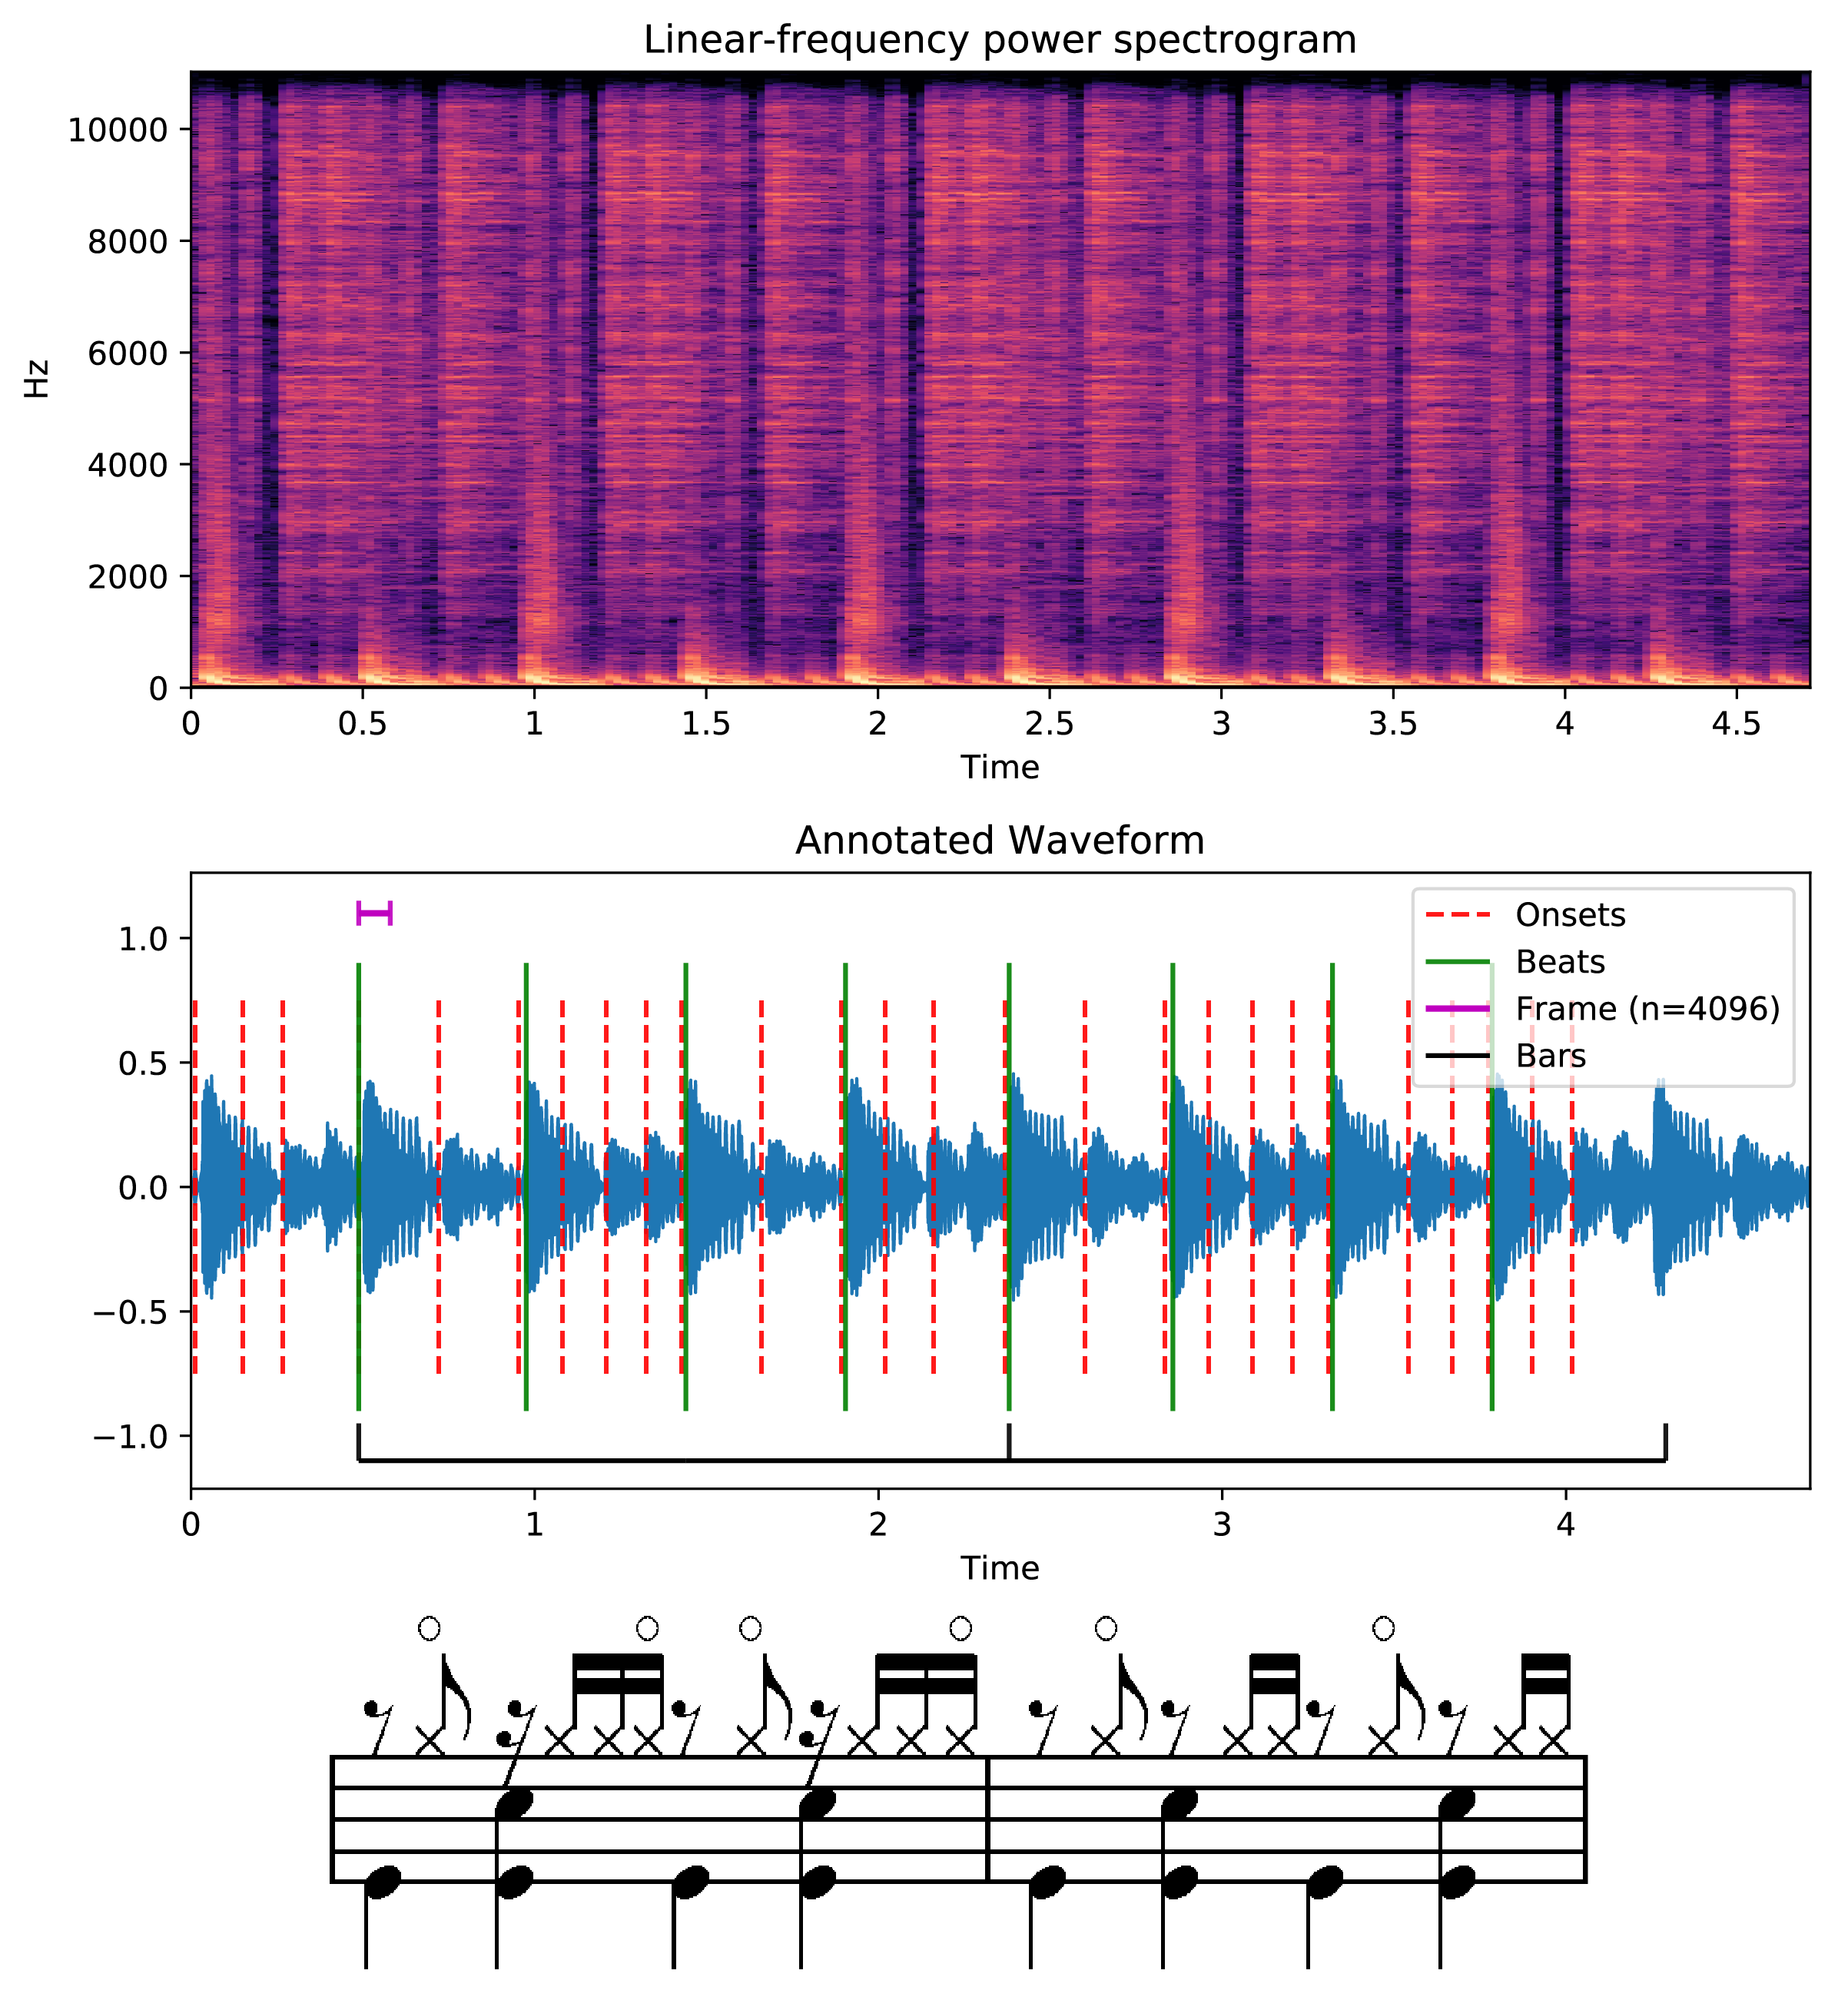
\includegraphics[width=0.75\textwidth]{ch05_pyconcat/figures/unit_plot.png}
	\end{center}
	\caption[Annotated Waveform, Spectrogram and Drum Transcription of ``My Sound'' by Joey Beltram (R\&S Records)]{Annotated Waveform, Spectrogram and (approximate) Drum Transcription of ``My Sound'' by Joey Beltram (R\&S Records)}
	\label{fig:beltram}
\end{figure}

\subsection{Framewise Segmentation}

At the lowest level of unit decomposition is the framewise unit. In granular synthesis many combinations of microsound timescales of typically 20-200 ms are combined to create dense masses of sound “clouds”. Granular synthesis systems typically control the recombination of these sounds in a parametric fashion; the user specifies or manipulates controls determining endmost pitch, length and envelope qualities. As \cite{Schwarz2003} notes, granular synthesis is “rudimentarily data-driven” but can be significantly augmented with pre-feature analysis - what we seek to achieve by performing concatenative synthesis. 

Granular synthesis is generally performed in the time domain, directly moulding and shaping the portions of the waveforms themselves using, for example, an amplitude envelope or windowing function based on Gaussian or linear patterns \citep{Roads1996, Roads2004}. Another option is to take frame sizes of orders of $2^n$ (512, 1024, 2048 etc). and transform them to the frequency domain using a \acrfull{fft}. Resynthesised signals can be reconstructed later in the time domain using the \acrfull{ifft} with overlap and add. While not an overly common approach to concatenative synthesis, it has been alluded to by \cite{Kobayashi}, \cite{Puckette2004}, \cite{An2012}, and some practical artistic applications have been summarised by \cite{Schwarz2006b}. The former describes how \acrshort{ifft} synthesis was used in the theatre piece \textit{La Légende des Siècles} (2002) to assemble \acrshort{fft} frames based on a target specification of pitch and energy. Frame-based segmentation and Fourier resynthesis are available as unit scale options in PyConcat, but have only been used and tested sporadically. The drawbacks of operating at this minuscule order of scale is the sheer level of data handling and computation it entails. Furthermore, if the composer is additionally working in the frequency domain they need to take extra care with continuity and phase, something a \acrshort{hmm} unit selection scheme further on would help address. 

%\begin{figure}
%	\begin{center}
%		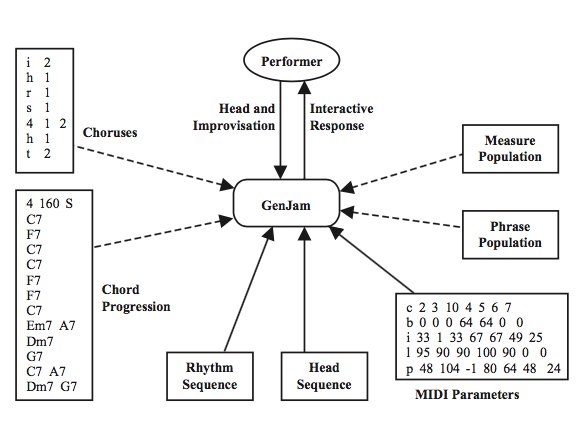
\includegraphics[width=0.8\textwidth]{ch03_symbolic/figures/genjam.png}
%	\end{center}
%	\caption[GenJam Architecture]{GenJam Architecture}
%	\label{fig:genjam}
%\end{figure}

\subsection{Onset Detection for Unit Decomposition}

%If microsonic grains are the de facto unit of scales for granular synthesis then the musical concept of a note with its, is the possibly the equivalent for concatenative synthesis. 
%
%Onset detection methods enables us to build a picture of where musical notes lie in a musical signal by looking for  

\subsubsection{Onset Detection Function}

At the heart of an onset detection algorithm lies the extrapolation of a detection function. The detection function, also referred to as the novelty, change or reduction function, is critical in reducing the complete audio signal from its higher sample rate to a lower frequency function of candidate peaks that reveal potential onsets. A detection function tries to detect moments of large change or flux, such that these drastic points of disparity in a signal quality like its energy signify the occurrence of a musical note or percussive transient. Time domain approaches work by taking a frame of audio samples of size $N$, summing the rectified absolute values (as in an envelope follower) or computing the \acrfull{rms}, then calculating the 1st-order differential of those values \citep{Laroche2003, Duxbury2002}.

More robust methods typically operate in the frequency domain. Critics of time domain methods point to its difficulty in recognising change of events in signals with high energy or noisy background \citep{Grzywczak2014, Eyben2010}. By operating in the frequency domain we can pick up on more information, in addition to energy/envelope changes, that might prove efficacious in the characterisation of a note event, such as the change of pitch revealed by its shifting spectrogram \citep{Schloss1985, Lerch2012}. Three of the most popular spectral methods include:

\begin{itemize}
\item Spectral Flux: Calculate the distance between two consecutive frames of the magnitude spectrum, using some distance measure such as Euclidean or absolute value.
\begin{equation}
\label{eq:Spectral Flux}	
F(n)=\frac{1}{N}\sum_{k=1}^{\frac{N}{2}-1}\sqrt{(X_{k}(n)-X_{k}(n-1)})^{2}
\end{equation}
\item Complex Flux: \cite{Bello2004} proposed extending the spectral flux method to incorporate phase information in addition to magnitude. By tracking the instantaneous phase of the complex spectrum, the real frequency can be calculated as per the phase vocoder \citep{Roads1996}. If the pitch of a note corresponds to a (mostly) steady state frequency then, in theory, deviations from the expected phase of a signal should reveal note events of signals where large energy changes are not such prominent indicators.
\item \acrfull{hfc}: Many percussive events are broadband in their frequency content, most notably those involving cymbals or snare sounds. To emphasise the contribution of higher frequencies to the novelty function, frequency bins of the spectrum can be weighted proportionally then summed to produce a framewise \acrshort{hfc} descriptor more tailored for percussive sounds.

\begin{equation}
\label{eq:High Frequency Content}	
F(n)=\frac{1}{N}\sum_{k=1}^{\frac{N}{2}-1}W_{k}|X_{k}(n)|^{2}
\end{equation}

\item Deep Learning Approaches: Reflecting recent trends in the arena of machine learning towards deep learning and application of neural networks, state of the art methods are also delivering some of the most promising results for creating usable novelty functions. \cite{Marolt2002} first proposed using a neural network, trained on a corpus of synthesised piano performances, to detect the presence of onsets in the amplitude envelopes of an \acrshort{iir} filterbank of 22 filtered signals.  \cite{Lacoste2007} proposed using supervised learning of a neural network trained to classify onset or non–onset in frequency representations of the signal, using an \acrshort{stft} and a Constant-Q Transform. Convolutional neural networks, such as those outlined by \cite{Schluter2013, Schluter2014} borrow from object classification tasks in computer vision research to analyse streams of spectrograms. Naturally, and in contrast to the more traditional signal processing methods, the success of supervised learning methods relies greatly on the data used for training.
\end{itemize}

\subsubsection{Thresholding and Peak Picking}
\label{sec:peak_picking}

The novelty functions returned by those methods described in the previous section returns candidate peaks, or, in the case of neural network oriented methods, probabilities of candidates that potentially correspond to onset times. To filter out spurious peaks and retain those local maxima, the novelty function needs to be processed through thresholding and application of a peak picking algorithm. 

Fixed thresholding retains only those peaks from the novelty function that exceed a constant threshold value. This works well for program material occupying smaller dynamic ranges, as in highly compressed music or percussive recordings. For material that varies in dynamics over time it is rather crude and inflexible - for such scenarios an adaptive thresholding procedure is preferable. Adaptive thresholding essentially computes another function that gives an instantaneous threshold value for each sample of the novelty function based on some analysis of that very function. Standard methods proposed by
\cite{Bello2005}, \cite{Dixon2006}, \cite{Bock2012a} and \cite{Bock2013}, choose a window of time $w$ around the current novelty function sample and derive a rolling average or low pass filtered version of the function, and reject peaks below some multiple of that threshold function.

Peak picking, as summarised by \cite{Bock2012a} can finally be applied by constraining the novelty function $F(n)$ to a set of criteria as in:

\begin{equation}
  \label{eq:peak_picking}
  \begin{gathered}
P(n)=max(F(n-w:n+w))\\
P(n)\geq mean(F(n-w:n+w))+\delta\\
n-n_{last}>\beta
  \end{gathered}
\end{equation}

where $n$ is the current frame number, $w$ is a window of frames around $n$, $\delta$ is a threshold multiplier to be applied to the rolling average and $\beta$ is used to reject potential onsets if they occur within a number of frames of a previously detected onset. Naturally, this set of criteria assumes that the source signal already exists in its entirety as in a pre-recorded sound file.

For real-time onset detection it is more challenging and less accurate as we do not have access to future frames of audio, unless some pre-delay is applied (as is done in look ahead limiters and processors that need some advance information in order to duck the signal). Even if no pre-delay is applied, novelty frames can only be compared to those captured in the past, which at least incurs a delay penalty of $w*N/SR$ milliseconds given frame length $N$ and sample rate $SR$ and frame window $w$.

\subsubsection{Evaluation of State of the Art Onset Detection Algorithms}

Our intention in this thesis is not to reinvent the wheel in basic building blocks for  musical signal processing, thus we propose no new methods for onset detection tasks. We do however, need to evaluate the state of the art methods currently available and compare their suitability for our needs in concatenative synthesis, which is documented in this section.

\paragraph{Datasets}

To evaluate the respective performance of each method, we gathered a number of datasets that are used in the literature and were made available, comprising:

\begin{itemize}
  \item ENST-Drums: Provided by Télécom ParisTech \citep{Gillet2006}, contains an audio-visual annotated dataset of performances by 3 professional drummers using multi-track studio recording in a variety of configurations (single hits, phrases and accompaniments) and a variety of styles including jazz and rock. 
  \item Modal (Musical Onset Dataset And Library): Hand annotated, contains 501 onsets across 71 files, with a mix of mostly monophonic events \citep{Glover2011}
  \item JKU: Contains 321 files with 27,774 total onsets. Compiled from a number of different sources by Sebastian Böck for evaluating his SuperFlux algorithm \citep{Bock2013}. The algorithm was developed especially to handle vibrato, and accordingly the dataset contains a large number of samples that purposely address vibrato, such as samples from opera or Western classical string technique.
\end{itemize}

\paragraph{Algorithms}

Three different exemplar onset detection methods, available in the Essentia \citep{Bogdanov2013} and the Madmom \citep{Bock2016} libraries, were integrated into our own PyConcat framework and their performances were estimated on the previously described datasets. The specifics of the algorithms themselves are explained as followed:

\begin{itemize}
  \item \textit{Essentia-OnsetRate:} Essentia’s “OnsetRate” algorithm combines the HFC and Complex domain novelty function detection methods. The two functions are multiplied by each other in order to emphasise those frames in agreement with each other. 
  \item \textit{Madmom-Superflux:} Madmom’s implementation of the Superflux algorithm as proposed by Böck et al. (2013). It expands on the spectral flux approach to handle program material that contains soft attacks, and instruments with vibrato tendencies such as strings, winds and the voice, that are difficult to capture using energy differences alone. 
  \item \textit{Madmom-CNN:} Uses a convolutional neural network to detect likelihood of onsets within a frame by frame basis \citep{Schluter2013, Schluter2014}. This algorithm achieved the highest scoring F-Measure and Recall and the second highest scoring Precision of the Onset Detection task as part of MIREX 2016.
\end{itemize}

\paragraph{Procedure}

Onsets were extracted using a batch procedure on all of the audio files with each algorithm using our PyConcat framework. For each audio file a single text file was produced with estimated onset times. These were then compared with the ground-truth annotations using the mir\_eval python package, a Python library for evaluating \acrshort{mir} related tasks according to \acrshort{mirex} guidelines \citep{Raffel2014}. An onset is defined as correctly identified if the time annotation is within +/- 50 ms of the ground truth annotation. Errors are categorised as either false positives or false negatives:

\begin{itemize}
  \item \textit{False Negative:} No onset estimation exists for a ground truth annotation
  \item \textit{False Positive:} An onset estimation outside the tolerance window for any ground truth annotation
\end{itemize}

Scores are computed for each file according to the standard information retrieval fractional measures of precision and recall as well as the F-measure, a derived measure that attempts to consolidate both previous measures for easy comparison of overall algorithms’ performance. Borrowing from the definitions provided in the sci-kit learn documentation\footnote{\url{http://scikit-learn.org/stable/auto_examples/model_selection/plot_precision_recall.html}} but adapted for the specific task of onset detection, we can define them as follows (where $T_p$ signifies true positives - correctly identified onset, and $F_p$ signifies incorrectly identified onsets).

\begin{itemize}
  \item \textit{Precision:} the fraction of total estimations that are correct:
\begin{equation}
\label{eq:Precision}	
P=\frac{T_{p}}{T_{p}+F_{p}}
\end{equation}  

  \item \textit{Recall:} the fraction of the total annotations that are correctly retrieved:
\begin{equation}
\label{eq:Precision}	
R=\frac{T_{p}}{T_{p}+F_{n}}
\end{equation}  

  \item \textit{F-Measure:} an aggregate score incorporating both precision and recall, defined as the harmonic mean of both:
\begin{equation}
\label{eq:Precision}	
F_{1}=2*\frac{P*R}{P+R}
\end{equation}  

\end{itemize}

\subsubsection{Results}

Results for all the files from each dataset were collated and statistics computed using mean and standard deviations, as summarised in \tabref{tab:onset_total_results}, while \figref{fig:onset_total_boxplots} provides corresponding box plots visually depicting the distributions. As is evident, the onset detector based on the \acrfull{cnn} is the highest scoring and most consistent of the onset detectors measured based on overall mean values and the small degree of spread in the box plots. Superflux also delivers excellent results, albeit with the introduction of more variance across samples. The combined methods present in Essentia's OnsetRate algorithm performed the most poorly, with the highest degree of spread across all measures.

{\renewcommand{\arraystretch}{1.5}
\begin{table} 
	\begin{centering}
		\begin{tabular}{lllllll}
\tabletop
    Algorithm & \multicolumn{2}{c}{Precision} & \multicolumn{2}{c}{Recall} & \multicolumn{2}{c}{F-Measure}\\
    & Mean & Std. Dev. & Mean & Std. Dev. & Mean & Std. Dev.\\
\tablemid
	\textbf{CNN} & \textbf{0.9208} & \textbf{0.1452} & \textbf{0.9073} & \textbf{0.1603} & \textbf{0.9062} & \textbf{0.1568}\\
	SuperFlux & 0.8719 & 0.1817 & 0.8702 & 0.1849 & 0.8550 & 0.1898\\
	OnsetRate & 0.8412 & 0.2166 & 0.7523 & 0.2287 & 0.7779 & 0.2128\\
\tablebot
		\end{tabular}
		\caption[Onset Detection Algorithm Results]{Onset Detection Algorithm Results}
		\label{tab:onset_total_results}
	\par \end{centering}
\end{table}

\begin{figure}
	\begin{center}
		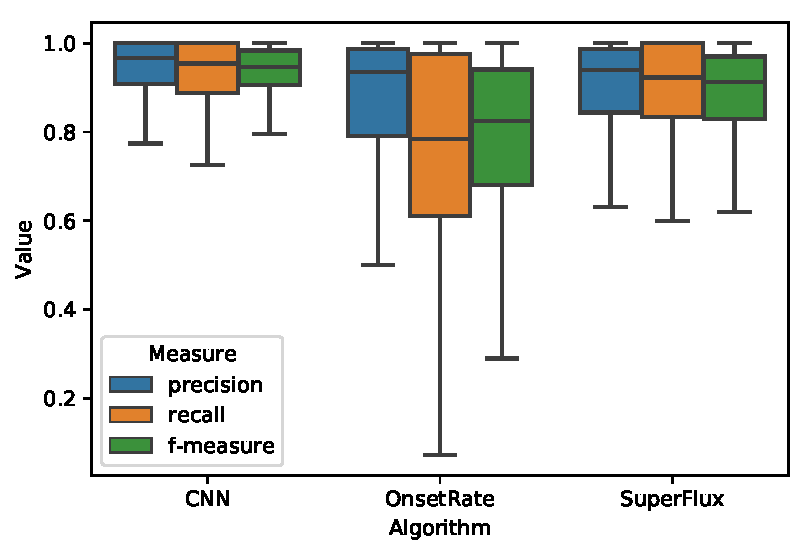
\includegraphics[width=0.75\textwidth]{ch05_pyconcat/figures/onset_total_boxplots.pdf}
	\end{center}
	\caption[Boxplots of Results for each algorithm and measure.]{Boxplots of Results for each algorithm and measure.}
	\label{fig:onset_total_boxplots}
\end{figure}

\tabref{tab:extended_onset_statistics} shows in more detail the statistics for each algorithm separated by the particular datasets evaluated and with the highest precision, recall and F-measure highlighted for each. It is interesting to note that all the algorithms deliver good results on the \acrshort{enst} dataset, which is entirely percussive. Superflux and \acrshort{cnn} perform much better on the \acrshort{jku} dataset on which it is been designed. These algorithms demonstrate their robustness on program material of all types, including sustained vibrato sounds as well as clear transient heavy percussive material.

\begin{sidewaystable}
	\begin{threeparttable} 
		\ra{1.1}
%		\small
		\begin{centering}
			\begin{tabular}{l l l l l l l l l l l}
				\tabletop
Algorithm & Dataset & Onsets & TP    & FP   & FN    & Precision & Recall & F-measure & mean & std \\
				\tablemid			
CNN       & ENST-1  & 8813   & 8057  & 697  & 756   & \textbf{0.921}     & \textbf{0.937}  & \textbf{0.921}     & 2.5  & 5   \\
          & ENST-2  & 10319  & 9738  & 484  & 581   & \textbf{0.945}     & 0.956  & \textbf{0.948}     & 1.6  & 5.4 \\
          & ENST-3  & 11019  & 10154 & 464  & 865   & 0.932     & 0.926  & 0.928     & 2.5  & 5.4 \\
          & JKU     & 25827  & 23293 & 978  & 2534  & \textbf{0.941  }   & \textbf{0.9}    & \textbf{0.916}     & -3.6 & 5.2 \\
          & Modal   & 501    & 418   & 122  & 83    & \textbf{0.774}     & 0.798  & \textbf{0.744}     & -3.9 & 3.2 \\
          \hdashline
Superflux & ENST-1  & 8813   & 7867  & 756  & 946   & 0.911     & 0.931  & 0.915     & -1.4 & 4.9 \\
          & ENST-2  & 10319  & 9553  & 549  & 766   & 0.94      & \textbf{0.957}  & 0.946     & -2.4 & 5.4 \\
          & ENST-3  & 11019  & 10018 & 481  & 1001  & \textbf{0.943 }    & \textbf{0.931}  & \textbf{0.935}     & -1   & 5.3 \\
          & JKU     & 25827  & 20382 & 2820 & 5445  & 0.847     & 0.809  & 0.811     & -5.9 & 5.9 \\
          & Modal   & 501    & 392   & 247  & 109   & 0.714     & \textbf{0.837}  & 0.706     & -4.2 & 3.5 \\
          \hdashline
OnsetRate & ENST-1  & 8813   & 6875  & 560  & 1938  & 0.901     & 0.875  & 0.871     & -5.7 & 7.1 \\
          & ENST-2  & 10319  & 8116  & 447  & 2203  & 0.941     & 0.872  & 0.895     & -6.3 & 7.3 \\
          & ENST-3  & 11019  & 8456  & 572  & 2563  & 0.91      & 0.868  & 0.875     & -5.4 & 7.4 \\
          & JKU     & 25827  & 15736 & 3335 & 10091 & 0.793     & 0.627  & 0.686     & -7.1 & 8.8 \\
          & Modal   & 501    & 333   & 213  & 168   & 0.719     & 0.784  & 0.732     & -4.6 & 4.6 \\
				\tablebot		
			\end{tabular}
			\par \end{centering}		
		\begin{tablenotes}
			\small
%			\item[] ABBREVIATIONS: NA=Not applicable; GD=Group Delay, PDE=Probability Density Estimate
		\end{tablenotes}
			\caption[Extended statistics for each algorithm by dataset]{Extended statistics for each algorithm by dataset}
			\label{tab:extended_onset_statistics}
	\end{threeparttable}
\end{sidewaystable}

The smaller Modal dataset appears to cause the most difficulty for all algorithms, but relaxing the tolerance time-window constraint from its default of 25ms to 50ms (actually the tolerance time used for \acrshort{mirex} tasks) improves the accuracy for all algorithms by a significant factor, suggesting it could be an issue of ground truth annotation style compared with the other datasets.

In terms of running time and overall algorithm performance, \figref{fig:onset_running_times} compares the averaged time and standard error (not visible due to low variance of < 1.0 s between consecutive runs). Recent trends towards deep learning solutions, while displaying promising returns in terms of accuracy over other supervised learning methods, frequently pale in comparison when considering efficiency and running times of the solution. Even with Madmom's built-in facility for distributing computational loads over multiple processors, the \acrshort{cnn} method performs much slower than the two flux-based approaches. Quite possibly the scale of the datasets is much larger than typical applications for concatenative synthesis, but the comparative performance of onset detection methods is an important point to consider when we look at real-time or at least quasi real time applications in due course.

\begin{figure}
	\begin{center}
		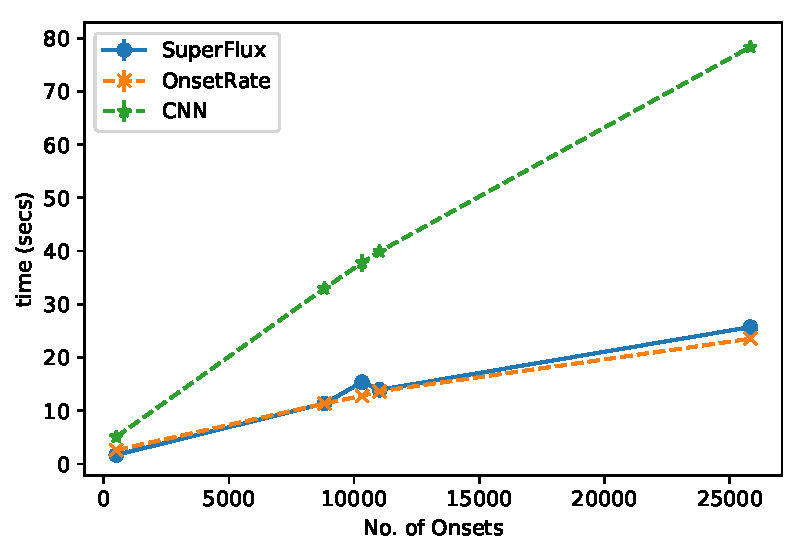
\includegraphics[width=0.75\textwidth]{ch05_pyconcat/figures/onset_running_times.pdf}
	\end{center}
	\caption[Mean and error of the running times of each algorithm over n=10 runs]{Mean and error of the running times of each algorithm over n=10 runs}
	\label{fig:onset_running_times}
\end{figure}

\subsubsection{Beat Tracking and Tempo Extraction}

It seems, from our impression of the literature, that in concatenative synthesis systems the typical unit length is of the onset (or to give it its perceptual equivalent, the note)  \citep{Schwarz2006, Frisson2010, Bernardes2013} - as extrapolated from a suitable onset detection process in the manner previously described. They are reasonably straightforward to compute and represent musically relevant building blocks for producing larger sequences of sounds. But larger musically relevant unit sizes are also a possibility.  Building on top of state of the art techniques in onset detection, \acrshort{mir} researchers are actively trying to coalesce this research with knowledge of tempo and rhythm to pursue algorithms that can perform automatic beat detection within signals.

Considering that most of the time we will be working at the onset scale of segmentation, analysis and selection, an extensive evaluation of state of the art methods in beat detection such as we performed for onset detection is outside of the scope of this thesis, but we do summarise some of the key works in this area including their respective \acrshort{mirex} results and expose them as possible unit decomposition options within our own framework. 

\figref{fig:beat_joplin} consolidates various rhythmic concepts from the onset to the bar level and how they relate to the waveform representation and timeline of a typical musical recording. Beats are defined as the perceptual tactus or dominant metrical pulse level that corresponds to where humans are most likely to tap their foot \citep{Jehan2005, Ellis2007a, Stark2009}. A stream of beats implies a certain tempo or \acrlong{bpm} measure of frequency that allow us to understand and compare the speed of musical works, and beat tracking and tempo detection are considered related tasks \citep{McKinney2007}. As \cite{Korzeniowski2014} note, there are many factors in interesting musical recordings that hinder computational facility to determine beats with ease, such as syncopation, hemiola and any other rudimental technique that seeks to thwart regular pulsation. By using tempo estimation and probabilistic prediction of where beats \textit{should} be when they aren't, beat tracking algorithms try to account for these factors. 

\begin{figure}
	\begin{center}
		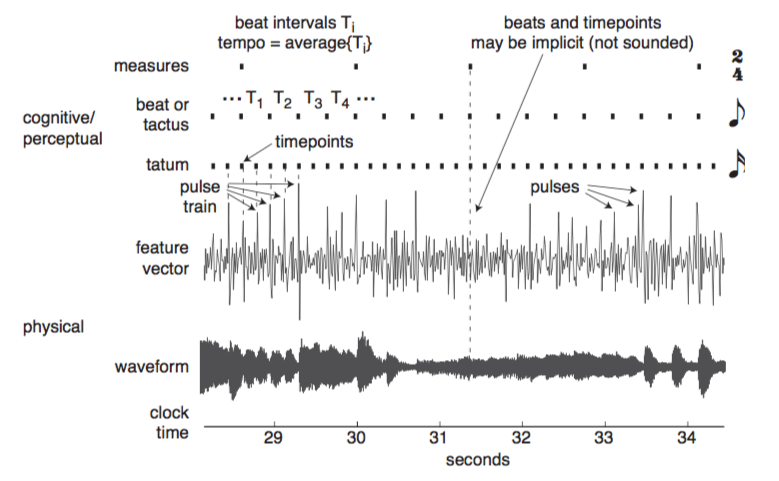
\includegraphics[width=0.9\textwidth]{ch05_pyconcat/figures/joplin.png}
	\end{center}
	\caption[Perceptual and Physical Concepts of Rhythm in a Scott Joplin Ragtime]{Perceptual and Physical Concepts of Rhythm in a Scott Joplin Ragtime. Image from \cite{Sethares2007}}
	\label{fig:beat_joplin}
\end{figure}

\cite{McKinney2007}, provide an excellent summary of the existing state of the art methods at their time of publication, organising the methods by differing implementations of a two-stage process. The process consists initially of the \textit{driving} stage, which produces features directly from the signal. This is followed by \textit{periodicity} stage, which outputs estimates of tempo and/or beats based on the analysis of those features \citep{McKinney2007}.

As was emphasised previously, beat tracking studies typically build on onset detection research, as beats essentially represent a perceptual and synchronous subset of onset locations in time. Thus most features \acrshort{hmm} derived for the driving stage consist of applying an onset detection method to produce candidate onset times \citep{Brossier2006, Dixon2006, Ellis2007a, Degara2012, Zapata2014} but not always. \cite{antonopoulos2007self} for example, use self-similarity of the \acrshort{mfcc} frames as its input. \cite{Degara2012}\footnote{Also one of the beat trackers available in Essentia} build upon their existing offering by integrating multiple input features that include energy flux, spectral flux, difference of Mel bands etc. Multiple candidates arising from the various feature inputs are resolved using a method of query by committee and maximum mutual agreement (MaxMA) proposed by the author previously in other work \citep{Zapata2012, Zapata2014}.

The periodicity stage, or where the features are filtered to produce beat locations is where the algorithms deviate the most from each other in terms of approach but many methods in the literature at least start from a probabilistic standpoint. Ellis (2006; 2007) uses onset detection followed by autocorrelation to get an initial estimate of the overall tempo of the track. This information is used by the beat-tracking module to compare the idealised beat times against computing the globally optimised set of beat times using \acrshort{ioi}s and dynamic programming in a manner not so far removed from that proposed by \cite{Alonso2007}. Degara also utilises a \acrshort{hmm}-based algorithm, augmented with an intrinsic framework that models sequences of non-beat states as well as beat states.

A multi-agent system for detecting periodicity has been employed by a number of investigators \citep{Goto2001a, Dixon2007, Oliveira2012}. In the case of Dixon, for instance, an initial tempo hypothesis and potential first beat from an initial set of onsets are assigned to several agents. Predicted beat times are then generated from the initial onset and hypothetic tempo, and onsets falling within a tolerated window of those predictive times are labelled as actual beats. A complex resolution system examines the degree of agreement between agents to decide on the final beat locations.

\paragraph{Current State of the Art and Deep Learning Approaches}

\tabref{tab:beat_tracker_results} shows the F-Measure scores for every algorithm submitted to the 2016 MIREX competition. The datasets under scrutiny include:

\begin{itemize}
  \item \textit{SMC} - 160 30-second excerpts of music in a variety of instrumentation and styles but with a stable tempo. 20\% of the examples contain non-binary meter.
  \item \textit{MAZ} - 367 Chopin Mazurkas with shifting tempos.
  \item \textit{MCK} - 217 tracks of roughly 40s long, with 19 “easy” and 198 “hard” excerpts from Romantic music, film soundtracks, blues, chanson and solo guitar.
\end{itemize}

{\renewcommand{\arraystretch}{1.0}
\begin{table} 
\footnotesize
	\begin{centering}
		\begin{tabular}{lllllll}
\tabletop
	Key & Name & Authors & \multicolumn{4}{l}{F-Measure}\\
		& 	   &		 & SMC & MAZ & MCK & Mean\\
	
				\tablemid			
BK1 & DBNBeatTracker.2016           & S. Böck,          & 56.8313 & 57.5286 & 63.6093 & 59.3231 \\
    &                               & F. Krebs          &         &         &         &         \\
BK3 & DBNDownBeatTracker            & S. Böck,          & 52.8343 & 73.8911 & 62.5299 & 63.0851 \\
    &                               & F Korzeniowski    &         &         &         &         \\
BK2 & CRFBeatDetector.2016  			& S Böck,           & 52.3142 & 55.1651 & 62.7315 & 56.7369 \\
    &         						& F Krebs           &         &         &         &         \\
SB9 & BeatRoot Vamp Plugin          & S. Böck           & 52.097  & 58.9357 & 63.8961 & 58.3096 \\
SB8 & QM Tempo Tracker              & S. Böck           & 49.8366 & 52.2792 & 63.8436 & 55.3198 \\
JZ1 & MultifeatureBT-Inf-7odf-Repet & J. R. Zapata      & 36.8192 & 50.63   & 52.6104 & 46.6865 \\
JZ2 & MultifeatureBT-Reg-7odf-Repet & J. R. Zapata      & 36.4073 & 47.874  & 53.2314 & 45.8376 \\
CD3 & QM Tempo Tracker              & C. Cannam,        & 33.663  & 49.6229 & 52.8758 & 45.3872 \\
    &                               & M. Davies         &         &         &         &         \\
CD2 & BeatRoot Vamp Plugin          & C.Cannam & 30.34  & 41.5218 & 52.6579 & 41.5066\\
 	&           					& S.Dixon 			&    &  &  & \\
\tablebot
		\end{tabular}
		\caption[Mirex 2016 Beat Tracking Results]{Mirex 2016 Beat Tracking Results}
		\label{tab:beat_tracker_results}
	\par \end{centering}
\end{table}

%\begin{sidewaystable}
%	\begin{threeparttable} 
%		\ra{1.1}
%		\begin{centering}
%			\begin{tabular}{lllllll}
%				\tabletop
%
%				\tablebot		
%			\end{tabular}
%			\par \end{centering}		
%		\begin{tablenotes}
%			\small
%%			\item[] ABBREVIATIONS: NA=Not applicable; GD=Group Delay, PDE=Probability Density Estimate
%		\end{tablenotes}
%			\caption[Extended statistics for each algorithm by dataset]{Extended statistics for each algorithm by dataset}
%			\label{tab:extended_onset_statistics}
%	\end{threeparttable}
%\end{sidewaystable}


Beat tracking is a significantly more complex task compared to onset detection, and evidently the results reflect this. Ranges of accuracy vary greatly across the different datasets and, while no single algorithm achieves the highest F-Measure, at least Böck and Korzeniowski’s DBNDownBeatTracker manages to attain the highest mean performance. Once again we see the headway deep learning based methods are making in all manner of pattern recognition and machine learning tasks, as this method relies on a recurrent neural network armed with a bank of resonant comb filters. 

\subsection{Future Directions - Mixing and Source Separation}

Most concatenative synthesis systems we have studied (including those techniques we propose) tend to consider the concatenation process in purely horizontal and temporally inclined terms.  Naturally, it is pertinent to question whether the same process can be applied systematically in the vertical dimension characterised by the frequency spectrum. Or, in more simpler terms - can we stack units on top of each other systematically in addition to chaining them in sequence? While not the focus of this thesis (but certainly a promising avenue for further study), we briefly summarise relevant topics of interest and  techniques that are or can be used.

\subsubsection{Vertical Selection with Mixture Models}

\cite{Hoffman2009} have outlined a system that seeks to recreate the target \textit{spectrum} by, as Coleman describes it \citeyearpar{Coleman2010}, \textit{superimposing} (using convolution) a series of spectra from a corpus. To reduce the complexity associated with high dimensionality, a search space reduction with a \acrfull{mcmc} is applied. 

In a version of AudioGuide by Hackbarth \citep{Hackbarth2013}, they also outline the system's facility for enabling ``layered sounds'' and ``vertically stratified complexes'' based on formulas \citep{Tardieu2008}  developed for a prior system in the OpenMusic environment called Orchidée or Automatic Orchestration Tool \citep{Carpentier2010}. The goal of their work is to transfer some of the principles of traditional orchestration (combining and arranging for instruments to create desired blends of timbre) to the realm of computer music by allowing prediction of mixtures as well as concatenations to match a target specification of a sound.

Hackbarth \citep{Hackbarth2010} describes the derived ``Subtractive Spectral Algorithm'' for superimposition. When an appropriate unit is selected from the corpus as a candidate match for the target, its time-varying Mel-amplitudes are subtracted from the target sound and a `residual' target spectrum remains. The unit selection procedure is performed repeatedly until it halts when the residual target spectrum energy falls below a certain threshold. The resulting units are then mixed together additively. A visual depiction of this over several mixtures can be seen in \figref{fig:spectrum_subtraction}. Clearly the algorithm tends towards selection of louder units initially, with gradually softer ones emerging as the subtracted target energy diminishes. 

\cite{Coleman2015} invokes the term ``mixtures'' to describe concatenative synthesis problems where the corpus might not have all the features to effectively simulate a target, but a carefully selected combination of them might. He uses the analogy of several single notes combining to form a chord, except the synthesis engine would use a weighted combination of superimposed frames mixed together.

\begin{figure}
	\begin{center}
		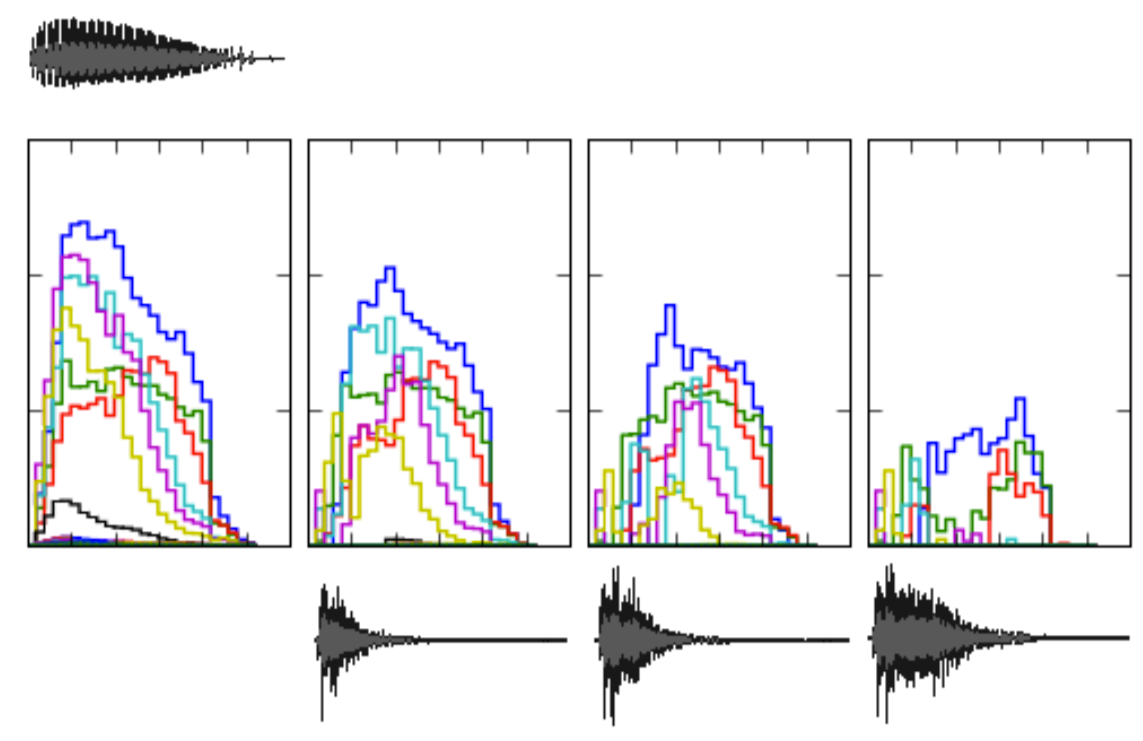
\includegraphics[width=0.75\textwidth]{ch05_pyconcat/figures/spectrum_subtraction}
	\end{center}
	\caption[Spectral Subtraction Algorithm in AudioGuide]{Visual depiction of spectral subtraction algorithm in AudioGuide. Image from \cite{Hackbarth2010}.}
	\label{fig:spectrum_subtraction}
\end{figure} 

\subsubsection{Vertical Segmentation with Source Separation}

As we highlighted previously in the case of the missing fundamental frequency, our auditory system is remarkable in its processing ability and inference engine. More remarkably,  perhaps, is its innate capacity for on the fly separation of real-time audio signals at will, or to give it its technical term, blind source separation. In pyschoacoustic auditory scene analysis research \citep{Bregman1994}, source separation is illustrated usually in terms of the ``Cocktail Party Effect'': how is a human, at a social event, able to separate voices from background noise and home in on particular conversations? In musical source separation this is even more elusive - consider picking out individual instruments in an orchestral passage, especially when, as \cite{Miron2017a} stresses, sources are likely to be correlated in time and frequency. Computational auditory scene analysis seeks to replicate this extraordinary human processing ability through digital signal processing means \citep{Wang2006}.

Initial efforts in computational source separation often involved matrix decomposition methods such as non-negative matrix factorisation, as demonstrated in the work of 
\cite{Fitz2004}. Fitzgerald's initial focus was on automatic drum transcription via source separation but later gained wider recognition with some some successful demixing and upmixing from mono to stereo of recovered archive Beach Boys recordings \citep{Fitz2004}. More recent state of the art approaches are once again successfully exploiting deep learning methods trained on large sets of musical data in genres like Western classical \citep{Miron2017a, Miron2017}.

Just as a concatenative synthesis system will use onset detection to split larger sound files into smaller units along the time domain, source separation opens up the possibility of theoretically segmenting complex sounds in the frequency domain according to instrument, or more accurately, \textit{streams} that hopefully contain related instruments (all depending of course on the material to be separated and the models upon which the system has been trained).

We envisage this as particularly useful in concatenative synthesis of drum rhythms. Perhaps a producer might want to decompose a number of kits into their constituent parts and mix and match with sounds from other sources. Mixing electronic drum sounds generated by a drum machine with naturally recorded acoustic drum sounds is a common strategy in dance music and source separation could prove invaluable here.

\section{Describing Sounds with Features}

\subsection{Temporal Descriptors}

\subsubsection{Intensity and Loudness}

Physically speaking, sound is a medium transporting mechanical energy via waves. In recorded media, analog or digital signals are converted to electrical and magnetic energy that push speakers backwards and forwards in a manner analogous to the original waveform captured.

Digital signals are essentially a series of amplitude values sampled at a particular sampling frequency. Taking the absolute value at an instantaneous sample point or the maximum absolute value over a window of samples gives us the peak amplitude. Unless the peak amplitude occurs frequently, in itself it is not a very useful indicator of the overall amplitude of the signal, thus the \acrfull{rms} is computed on the window of samples to get a better statistic of the general power of the signal \citep{Puckette2006}:

\begin{equation}
\label{eq:rms}	
A_{RMS}\{x[n]\} = \sqrt{\frac{1}{N}(x[1]^2, x[2]^2,..., x[N]^2}
\end{equation}

where $N$ is the length of the discrete time signal $x$ and $x[n]$ are the individual samples. Most other works we have encountered related to concatenative synthesis use \acrshort{rms} as their principal loudness descriptor, particularly \cite{Sturm2004} and \cite{Bernardes2013}, but \cite{Jehan2005} computes his loudness descriptor from energy in the frequency domain.

Human perceptual response to increments in amplitude is intrinsically logarithmic, thus to aid relative comparisons and metering purposes, amplitude values are often computed as a ratio of some reference value and reported using the \acrfull{db} scale, as Puckette \citeyearpar{Puckette2006} indicates. 

\begin{equation}
\label{eq:decibel}	
d = 20\log_{10}{\frac{a}{a_{0}}}
\end{equation}

\begin{figure}
	\begin{center}
		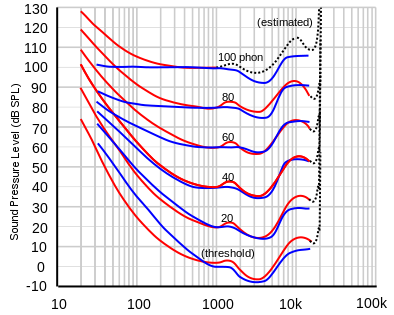
\includegraphics[width=0.75\textwidth]{ch05_pyconcat/figures/fletcher_munson.png}
	\end{center}
	\caption[Fletcher-Munson Curves]{Equal-loundness curves in red with ISO revisions in blue. Image from Wikipedia.}
	\label{fig:fletcher}
\end{figure}

Intensity, power, energy etc. are all \textit{objective} physical concepts. We use the term \textit{loudness} to describe the subjective human perceptive experience that we feel when exposed to intensity of sound. As \cite{Lerch2012} points out, the decibel is neither a true indicator of loudness because "equal-sized steps on the decibel scale are not perceived as equal-sized loudness steps by human listeners", or as \cite{Stevens1955} puts it more succinctly: "equal steps do not sound like equal steps".

Perceived loudness depends on many factors, and, as the long established  Fletcher-Munson equal-loudness contours reveal, it is heavily skewed by frequency. Introduced in the 1930s \citep{Fletcher1933}, subsequently revised as an ISO standard in \cite{countours}, this set of curves (\figref{fig:fletcher}), produced using listening tests, estimates frequency versus sound intensity pressure level where listeners perceive loudness to be roughly equal. To make matters worse, these curves change according to overall intensity, such that at  the difference is more pronounced between frequency ranges at low intensities, while gradually flattening out as intensity increases.

Luckily, more pyscho-acoustically aware measures that take into account such subtleties and phenomena are implemented and available as content analysis features. The \acrfull{ebu}, for example, proposes the \acrshort{ebu} R 128 metering standard in an effort to enforce normalisation consistency across differing programme material in broadcasts\footnote{And combat au-fait advertising and music producers exploiting dynamic range compression to make their products stand out from others.} \citep{ebu, Lerch2012}. It consists of a perceptually tuned K-weighting filter followed by mean square power estimated at momentary, short-term and longer-term intervals.

We are using content analysis mainly for our unit selection algorithm to compute similarity between feature vectors so advanced metering standards like the \acrshort{ebu} R 128 are a bit complex for our purposes, and we haven't seen any instances of its usage in synthesis systems. Another, more basic loudness descriptor available in Essentia's library implements Stevens' Power Law. Stevens' Power Law arose out of efforts to improve on the Weber-Fechner pyschophysics laws that relate changes in physical stimuli with perceptual response to those changes \citep{Stevens1975, Reiss2001}. It is elegant:

\begin{equation}
\label{eq:stevens}
S(i)=k.i^{n}
\end{equation}

where $S$ is the sensation (perceived magnitude), $i$ is the intensity, $k$ is a unit dependent constant and $n$ is an exponent that depends on the stimulus. Through many perceptual experiments, Stevens produced exponents for a wide variety of physical stimuli, ranging from brightness of light to taste when exposed to sucrose or salt, for example. In the case of loudness, that exponent is estimated at 0.67 \citep{Stevens1975}, and in Essentia it is implemented as the signal energy \eqref{eq:energy} raised to that exponent \eqref{eq:stevens_loudness}.

\begin{equation}
\label{eq:energy}
E\{x[n]\}= \sum_{n=-\infty}^{n=\infty}|x[n]|^{2}
\end{equation}

\begin{equation}
\label{eq:stevens_loudness}
L\{x[n]\}= E\{x[n]\}^{0.67}
\end{equation}

We use the Stevens' Law based descriptor in our systems as it provides (in our view) an acceptable trade off between ease of integration and grounding in some awareness of perceptual theory. Loudness is a scalar feature, and one of two features we compute solely in the time domain. It is an extremely important quantity that is essential in ensuring that units selected match not only the overall naturalness and dynamics of the target sound, but also remain consistent over the continuous trajectory of the sequence subsequent to concatenation. 

\subsubsection{Log-Attack Time}

The evolution of the energy in a sound is frequently described in terms of its attack, decay, sustain and release envelope \citep{Peeters2004b, Kim2006, Brossier2004a} and is a central facet of modular and digital sound synthesis \citep{Russ2004}. 

Technically it is resolved by taking the logarithm of the time taken from $t0$ to $t1$, where $t0$ is some initial energy percentage of the envelope, while $t1$ is some maximal percentage of the envelope, indicating the end of the attack and the start of the decay or sustain portion (\eqnref{eq:lat}).

\begin{equation}
\label{eq:lat}
lat = log(t1-t0)
\end{equation}

Why do we take the logarithm? Well, just like other perceptual responses to physical stimuli  studies have found higher degrees of correlation in studies examining timbre discrimination when the logarithm is applied.\citep{McAdams1995, McAdams1999, Agres2016}. The log attack time is obviously very useful for discriminating sounds that have distinctive attack profiles \citep{Herrera-Boyer2003}, such as the flute versus a snare drum for example, so naturally this feature makes more sense for ``one-shot'' instrumental classification versus excerpts of recordings for the purposes of genre detection.

\subsection{Spectral and Timbral Descriptors}

Timbre is an extremely complex and elusive aspect of sound for a very simple reason: it is a quality that is likely an emergent property, with indeterminate dimensionality \citep{Elliott2013, Siedenburg2017} or even dimensionality exclusive to a particular timbre \citep{Krumhansl1989}. A typical definition usually follows along the lines of that issued by the Acoustical Society of America:

\blockcquote[]{ansi}{``\textit{That attribute of auditory sensation which enables a listener to judge that two nonidentical sounds, similarly presented and having the same loudness and pitch, are dissimilar}''} 

An elegant distillation undoubtably, but other researchers point out \citep{Siedenburg2017} there is difficulty in these so-called ``wastebasket'' reductionist attempts that leave us none the wiser:

\blockcquote[]{McAdams1979}{``\textit{timbre tends to be the the psychoacoustician's multidimensional waste-basket category for everything that cannot be labeled pitch or loudness.}''} 

\blockcquote[]{Bregman1994}{``\textit{This is, of course, no definition at all. [...] The problem with timbre is that it is the name for an ill-defined wastebasket category. [...] I think the definition [...] should be this: ‘We do not know how to define timbre, but it is not loudness and it is not pitch.’ [...] What we need is a better vocabulary concerning timbre.''}}

\subsubsection{Fourier Analysis (and Synthesis)}

A working knowledge of Fourier analysis and awareness of the first point \citep{ansi} does give a starting point for many systems that deal with timbre. Fourier's theorem says that any sound in the time domain can be transformed to a sum of sinusoid functions and associated amplitudes in the frequency domain or spectrum \citep{Roads1996}. Overlapping frames of samples taken from a longer signal can be multiplied by a suitable window function, giving a better indication of the evolution of the sound over time, in what is known as a the \acrshort{stft} or spectrogram (if observing just the magnitude) \citep{Collins2010}(\eqnref{eq:stft}).

\begin{equation}
\label{eq:stft}
X[n,k] = \sum_{n=0}^{N-1}\{w[n]x[mH+n]e^{-j2\pi kn/N}\}
\end{equation}

where $w[n]$ is a window function, $H$ is a hopsize, $m$ is the hop number and $k$ is the frequency bin number. If two sounds have the same pitch and loudness - or objectively speaking, the same \textit{perceived} fundamental frequency and amplitude - then perhaps examining the spectrogram should give us a better indication as to what discriminates the two. Examining different sounds using Fourier analysis shows us how different sounds are made up of spectrograms that not only have different magnitudes at different peaks, but also these magnitudes and peaks can evolve over time according to unique envelopes. These peaks in the spectrum are known as partials. When examining musical signals in a spectrum, we call the first partial that is at the lowest frequency in the signal as the fundamental frequency or first harmonic\footnote{Though the human cortex has the extraordinary ability to ``fill in'' a missing fundamental (or \textit{pitch of residue} \citep{Weihs2009}) for a complex harmonic tone even when absent.}. Any partial above this fundamental frequency that is related to the fundamental by an integer ratio is furthermore labelled as the second, third, fourth harmonic and so on, forming the harmonic series \citep{Puckette2006}.

Fourier theory also gives us a constructionist framework for additive synthesis of sounds - by carefully mixing parameters of a bank of sinusoids we can arrive at more complex sounds and even try to mimic some of those found via analysis. But additive synthesis gets very complicated very quickly. Besides having to keep track of large sets of parameters, computing huge banks of sinusoid functions concurrently is computationally expensive. Typical analog and digital synthesisers in the music producer's arsenal approach the problem from the other direction. Complex signals such as squares, sawtooths, or certain shapes drawn in a wavetable are filtered and sculpted to arrive at the desired sound in a process known as \textit{subtractive} synthesis. \acrfull{fm} synthesis also famously uses parametric control of a carrier signal's frequency modulated by a modulation frequency to produce a wide palette of sounds, but its minimal set of parameters can prove notoriously complex and difficult in trying to fathom a preconceived sound. 
 
Getting back to spectral and timbral analysis\footnote{It's also worth mentioning spectralism here, a post-Serialist movement in European composition that ran tandem to the burgeoning minimalism across the Atlantic. At \acrshort{ircam}, Gérard Grisey and Tristan Murail harnessed computational analysis of spectra to inspire dense scores on chamber works such as \textit{Les espaces acoustiques} and \textit{Gondwanda} \citep{ross2007rest, Harvey2000}}, the Fourier transform and its spectrogram is a central concept in musical signal processing, and while usually not employed directly as a raw feature in itself, it forms the basis for numerous other algorithms (recall its role in flux-based onset detection) and descriptors in \acrshort{mir} literature and systematic practice which we will now turn to. 

\subsubsection{Spectral Centroid}

The spectral centroid gives a scalar value indication of the ``centre of gravity'' in the spectrum of the signal, and as such is computed as the weighted mean of the spectral bin frequencies, with the magnitudes acting as weights (\eqnref{eq:centroid}).

\begin{equation}
\label{eq:centroid}	
c = \frac{\sum_{i=1}^{N}f(i)m(i)}{\sum_{i=1}^{N}m(i)}
\end{equation}

where $f(i)$ is the centre frequency of bin $i$, and $m(i)$ is its associated magnitude. It is considered a robust and reliable indicator of the perceptual ``brightness'' of a sound \citep{Schubert2004}, and is utilised in a variety of systems that classify sounds. In \figref{fig:spectral_features} we can see three different impressions of a drum pattern (programmed in Ableton with a TR-909 preset). The top image shows the ``symbolic'' step pattern notation as would be used in a \acrshort{midi}-based production environment such as Ableton. The middle image the shows the rendered waveform (or time-domain representation) of the drum pattern. Finally in the bottom image the log frequency/ power spectrum shows the frequency domain impression of the signal. Overlaid on the spectrogram, in green, is the spectral centroid computed for every frame of the spectrogram. As we can see the centroid follows the envelope shape of the centre of energy for the spectral evolution of the signal.

\begin{figure}
	\begin{center}
		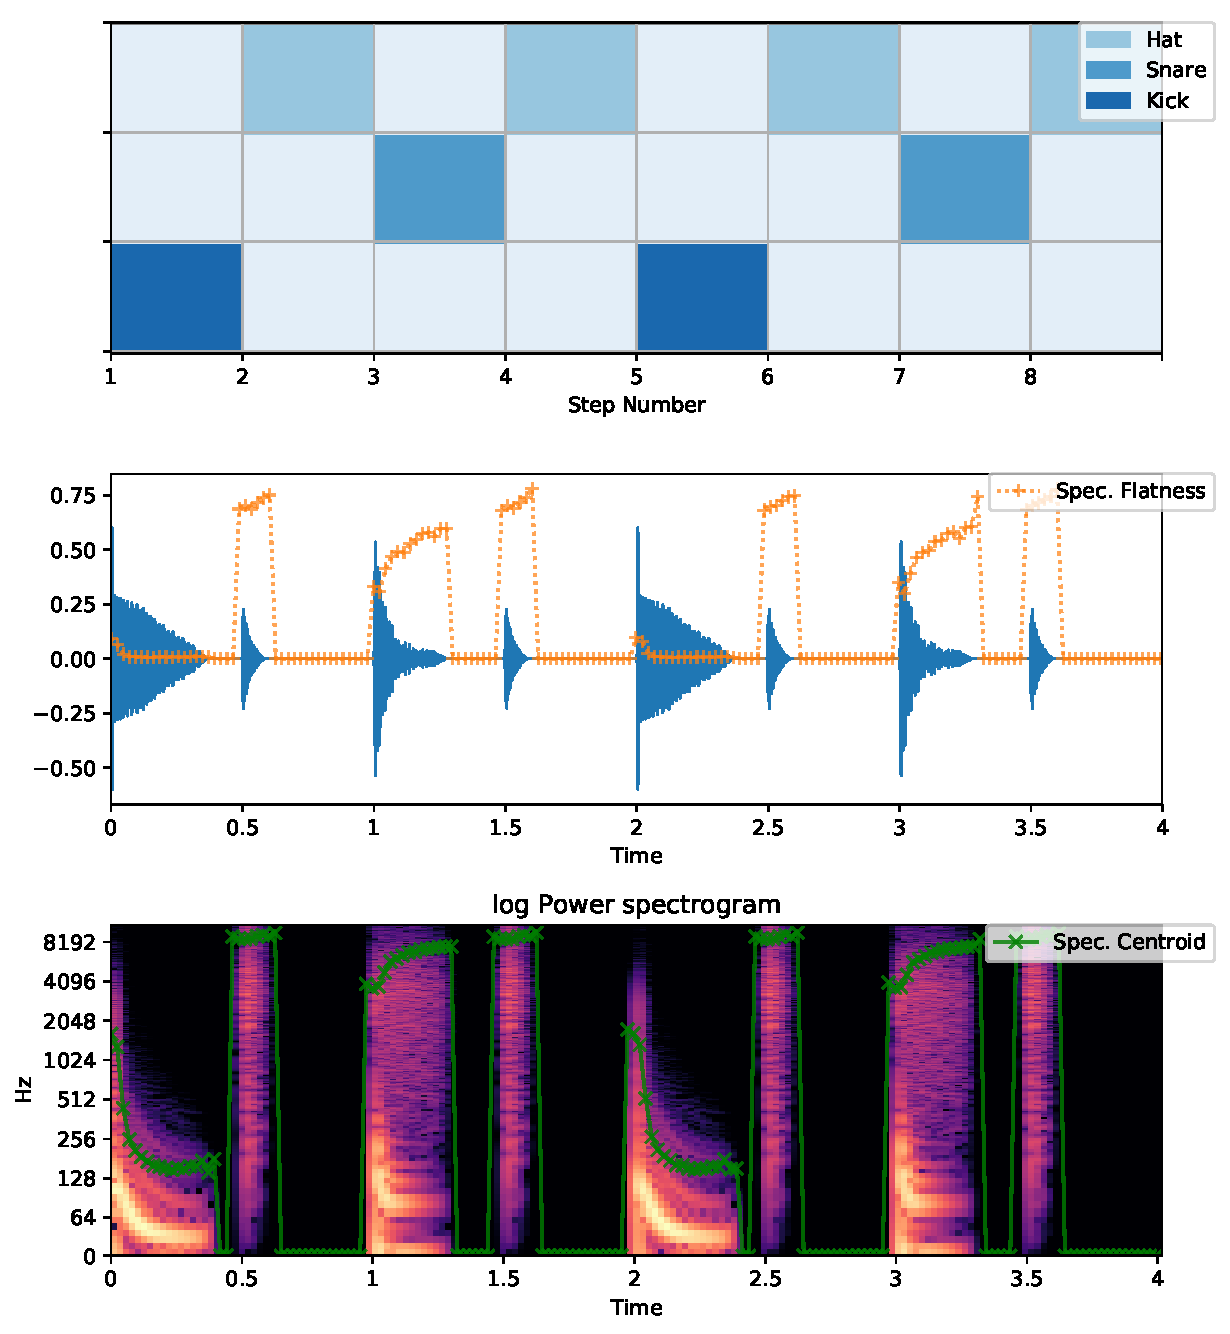
\includegraphics[width=0.85\textwidth]{ch05_pyconcat/figures/spectral_features.pdf}
	\end{center}
	\caption[Spectral features of a drum pattern]{Symbolic grid representation of drum pattern (top). Waveform with spectral flatness (middle). Audio spectrogram with spectral centroid (bottom).}
	\label{fig:spectral_features}
\end{figure}

\subsubsection{Spectral Flatness}

Another feature computed on the spectral profile at each frame is the spectral flatness. The spectral flatness or ``Wiener entropy'' gives an indication of how peaky or flat the spectrum is. Peaky spectra tend towards 0.0 and are indication of more harmonic or tonal sounds while a perfectly flat spectrum of 1.0 indicates stochastic noise. Mathematically it is defined as the geometric mean of the bin amplitudes of the spectrum divided by the arithmetic mean of the same bin amplitudes (\eqnref{eq:flatness}). 

\begin{equation}
\label{eq:flatness}	
f=\frac{\sqrt[N]{\prod_{n=0}^{N-1}X(n)}}{\frac{\sum_{n=0}^{N-1}X(n))}{N}}
\end{equation}

In \figref{fig:spectral_features} in the middle image we observe the spectral flatness has been plotted against the waveform view. Since the range bounds of spectral flatness fall between 0.0 and 1.0 this makes more sense than trying to normalise it into a range that can be plotted easily against the spectrogram. In any case, it can be clearly seen how the flatness function, while reasonably correlated with spectral centroid overall, deviates and approaches the origin for the kick timbre. While percussive sounds are generally considered to be less ``tonal'' overall compared to their non-percussive counterpoints, low frequency membranes such as kick drums and tom-toms do exhibit more discernible pitch compared to the clearly more broadband profiles in the snare and hi-hat, and this is evident simply by looking directly at the relevant time points in the spectrogram. Indeed, typical recipes for synthesising electronic kick drums (such as those found in Roland gear) often suggest combining a sine wave with an envelope controlling a sharp decay in frequency with some short impulse of filtered noise (to create a percussive ``click'') \citep{Risset1999, Reid2002}.

\begin{figure}
	\begin{center}
		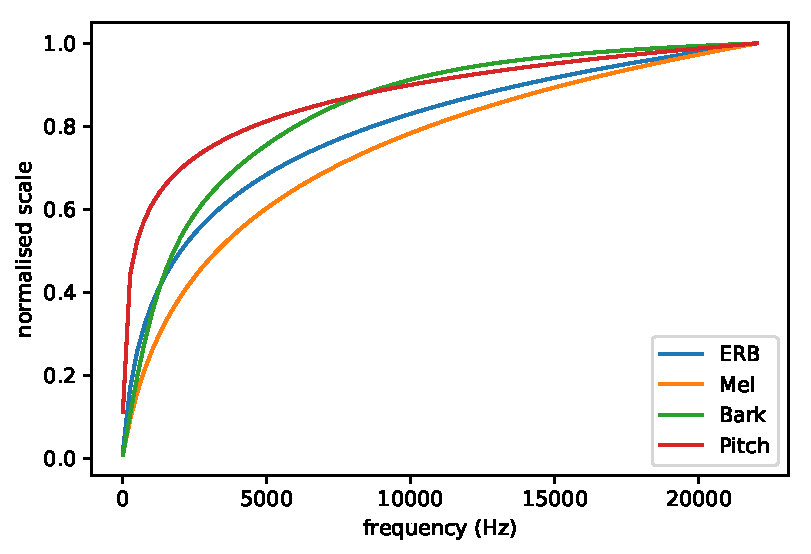
\includegraphics[width=0.8\textwidth]{ch05_pyconcat/figures/scale.pdf}
	\end{center}
	\caption[Perceptual Scales for Audible Range]{Different perceptual scales (normalised) for the audible frequency range}
	\label{fig:perceptual_scales}
\end{figure}


\subsubsection{Cepstrum Analysis}

Effective analysis of complex timbres in musical and natural signals typical employ derived features that exploit some understanding of human perception. The human ear is typically believed to respond to the dynamic limits of 0-120dB and frequency ranges of roughly 20Hz - 20kHz\footnote{Thanks to many years of ignoring advice on earplugs, I strain to hear anything above 14kHz!}\footnote{A famous anecdote recounted by revered console designer Rupert Neve claims that Beatles engineer Geoff Emerick discovered an anomaly in a desk that was attributed to an oscillation at 54kHz \citep{Winer2012}, but later they concede that this was probably due to suboscillatory spillage into the audible range.}. But as we know, human sensation to stimuli is not linear - we don't perceive phenomena in the same way physical measurements are made. The upshot of this is that important information "spreads out" at higher frequencies compared to the more compact resolution of the lower bands.

Pitch is the perceptual description we give to the way our brains organise frequency for the purposes of music. If a tone is perceived to have a pitch at a particular frequency, doubling the frequency of that tone is perceived as the same pitch except one \textit{octave} unit higher.

Depending on when (what era) and where (what culture) you were born in the world, how that octave is divided up can be very different (take for example, just intonation or Indian art music). Assuming the chromatic scale based on equal temperament tuning, its octave is divided into 12 semitones using the following formula:

\begin{equation}
\label{eq:pitch}	
p = 69 + 12 * \log_2(\frac{f}{440})
\end{equation}

What is essentially happening here is a type of frequency warping - compressing sound frequency onto a smaller, perceptual scale that is more tuned for human perception and cognition. In fact, there are other frequency warping formula in the literature that serve to warp frequency according to some conceptually pyschoacoustical or perceptual scale. \figref{fig:perceptual_scales} shows a number of perceptual scales and their normalised output with frequency in Hz as input, notice how they all exhibit a sharp rise that flattens out as it approaches the upper bounds of human response to frequency.

Cepstrum analysis has been one of the most dominating analysis techniques in speech processing for a long time. The word cepstrum itself rearranges the first four letters of the word spectrum, and has been described variously as a type of ``spectrum of a spectrum''. Its usage within speech analysis stems from the fact that it allows to separate the two dominant spectra of a vocal sound - the initial glottal impulse excitation and the slower resonance of the vocal tract \citep{Roads1996, Kim2006}.

To compute cepstrum is comparatively straightforward. The \acrshort{fft} of the signal is taken as normal. The magnitude is retained and the log magnitude spectrum is computed. Finally, the inverse \acrshort{fft} (\acrshort{ifft}) is applied to the log magnitude spectrum. However, normally some frequency warping formula is applied to compress the spectrum in some pyschoacoustic and perceptually motivated manner, and it is here we derive the family of features that include \acrfull{mfcc}, \acrfull{bfcc} and \acrshort{gfcc} (Gammatone Frequency Cepstrum Coefficients warped according to Equivalent Rectangular Bands \citep{Shao2009}). \figref{fig:bfcc_mfcc_gfcc_compared} shows the computed coefficients and the ranges of these features side by side for visual comparison.

\paragraph{MFCCs}

MFCCs are the most common flavour of cepstrum analysis \citep{Kim2006}. \acrshort{mfcc}s use a Mel-spaced filterbank to convert the spectrum to energy in Mels (\figref{fig:perceptual_scales}). The Mel scale, based on perceptual experiments performed by \cite{Stevens1937}, provides a mapping from frequency to Mel pitches that listeners have deemed equal to each other in distance, in a manner similar to the equal-loudness contours previously. While not visible in the normalised representation in \figref{fig:perceptual_scales}, as \cite{Kim2006} notes, the Mel scale and frequency are actually linearly correspondent up until around $500Hz$, at which point it begins to space out across the upper range.

The formula for converting frequency in Hz to Mel pitches is given by:

  \begin{equation}
	\label{eq:mel}	
	m = 2595\log_{10}(1+\frac{f}{700})
	\end{equation}
	
\begin{figure}
	\begin{center}
		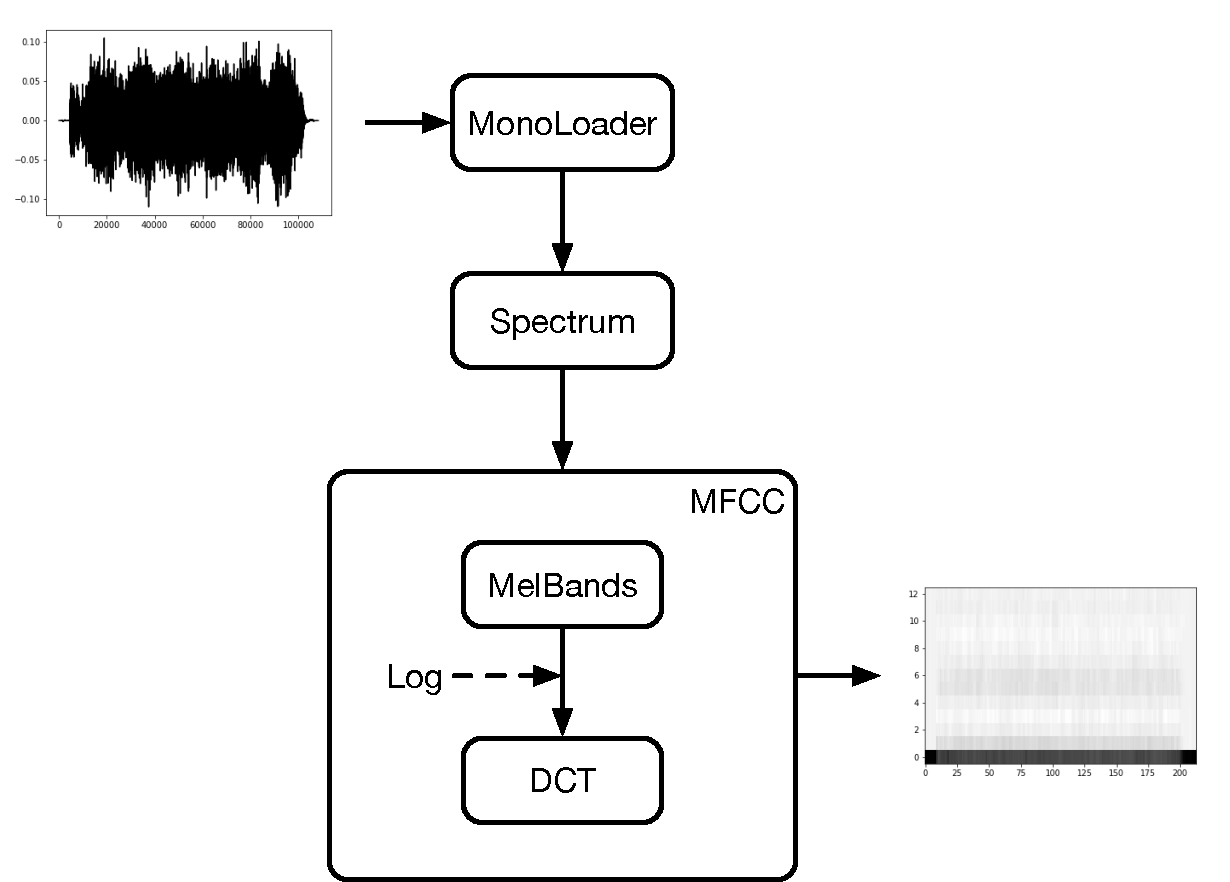
\includegraphics[width=0.9\textwidth]{ch05_pyconcat/figures/mfcc_diagram.pdf}
	\end{center}
	\caption[Signal Flow and Essentia Algorithm Graph for MFCC Computation ]{Signal Flow and Essentia Algorithm Graph for \acrshort{mfcc} Computation }
	\label{fig:mfcc_diagram}
\end{figure}	

To compute the \acrshort{mfcc}s the following steps are taken \citep{Logan2000, Lyons2015}:

\begin{enumerate}
  \item Perform the STFT as given by \eqnref{eq:stft}.
  \item Get the magnitude given by $M(n) = |X(n)|$.
  \item Get the log magnitude given by $L(n) = log(M(n))$.
  \item Warp the log-magnitude spectrum to the Mel scale using 40 triangular filters according to \eqref{eq:mel}.
  \item Finally take the Discrete Cosine Transform \eqref{eq:dct} of the Mel-Frequency log spectrum to obtain the 40 MFC coefficients.
  \begin{equation}
	\label{eq:dct}	
	X_k=\sum_{n=0}^{N-1}x_n cos [\frac{\pi}{N}(n+\frac{1}{2})k]
	\end{equation}
\end{enumerate}

\figref{fig:mfcc_diagram} shows how MFCC extraction is performed in the Essentia environment, showing the signal flow through the various stages, conceptually encapsulated as algorithms. Essentia processes data in a graph-based network, not unlike signal flow languages such as \acrshort{pd} and Max; objects (or algorithms) are connected virtually to each other, and more complex algorithms (composite algorithms) can be assembled by combining other algorithms with processing routines. This is actually the case with the \acrshort{mfcc} algorithm, which as can be seen in the figure receives a spectrum, uses the MelBands algorithm to filter the spectrum, computes the logarithm then finally outputs the \acrshort{mfcc} result from the \acrshort{dct} algorithm. 

\begin{sidewaysfigure}
	\begin{center}
		\includegraphics[scale=0.70]{ch05_pyconcat/figures/wave_spec_mfcc_bfcc.pdf}		
		\end{center}
		\caption[Waveform, Spectrogram, BFCC, MFCC and GFCC impressions of the ``Amen Break'' drum solo from ``Amen Brother'']{Waveform of drum break from ``Amen Brother'' (top-left). Power Spectrogram of waveform (top-right). BFCC coefficients 1-13 by frame number (bottom-left). MFCC coefficients 1-13 by frame number (bottom-centre). GFCC coefficients 1-13 by frame number (bottom-right)}
	\label{fig:bfcc_mfcc_gfcc_compared}
\end{sidewaysfigure}

%\begin{figure}
%	\begin{center}
%		\includegraphics[width=1.0\textwidth]{ch05_pyconcat/figures/wave_spec_mfcc_bfcc.pdf}
%	\end{center}
%	\caption[Waveform, Spectrogram, MFCC and BFCC Representations]{Waveform of drum break from ``Amen Brother'' (top-left). Power Spectrogram of waveform (bottom-left). MFCC coefficients 1-13 by frame number (top-right). BFCC coefficients 1-13 by frame number (bottom-right).}
%	\label{fig:wave_spec_mfcc_bfcc}
%\end{figure}


Interpreting exactly the meaning of each of the MFCC coefficients (\figref{fig:bfcc_mfcc_gfcc_compared}) is not as simple as is examining each bin of an \acrshort{fft} for instance. However, in most discourse dealing with \acrshort{mfcc} analysis the emphasis appears to be on the first 13 coefficients as higher order coefficients are considered to contain increasingly redundant information \citep{Logan2000}. Additionally, the first coefficient is usually correlated most with the energy of the signal and is also frequently omitted in further usage.  We follow suit also, since we are already computing energy using the specially designed Stevens' Power Law descriptor.

{\renewcommand{\arraystretch}{1.5}
\begin{table} 
		\begin{tabular}{l l l l l}
\tabletop
Library & Language & MFCC & BFCC & GFCC\\
\tablemid
Aubio  \citep{Brossier2006} & C \& Pd & Yes  & No & No\\
MIR Toolbox \citep{Lartillot2008} & Matlab & Yes  & No & No\\
LibXtract \citep{Bullock2007} & Pd & Yes  & No & No\\
TimbreID \citep{Brent2010} & Pd & Yes  & Yes & No\\
Essentia \citep{Bogdanov2013} & C++ \& Python & Yes  & No & Yes\\
Librosa  \citep{Mcfee2015} & Python & Yes  & No & No\\
Madmom \citep{Bock2016} & Python  & Yes  & No & No\\
\tablebot
		\end{tabular}
		\caption[Availability of MFCC, BFCC and GFCC Descriptors in Common Audio Labelling Libraries]{Availability of \acrshort{mfcc}, \acrshort{bfcc} and \acrshort{gfcc} Descriptors in Common Audio Labelling Libraries.}
		\label{tab:library_summary}
	\par
\end{table}


\subsubsection{BFCCs}

If the \acrshort{mfcc} feature uses the Mel scale for warping the spectrum, then the extremely related \acrshort{bfcc} feature differs only in its warping procedure using the Bark scale. The Bark scale maps frequency to Barks using this formula:

\begin{equation}
\label{eq:High Frequency Content}	
b = [26.81*\frac{f}{(1960-f})]-0.53
\end{equation}

Aside from that the procedure is pretty much the same as for \acrshort{mfcc} computation. Overlapping filterbanks tuned to the the bark scale are applied to the spectrum, the logarithm is applied and finally the \acrshort{dct} transform is performed to produce the coefficients.

The \acrshort{bfcc} feature has not enjoyed the same level of popularity as its \acrshort{mfcc} counterpart, most probably since it is not available as an extractor in the major feature extraction and analysis environments (\tabref{tab:library_summary}).

The Mel scale is an extremely robust and reliable warping scale for many applications, but it is still prudent to experiment with other feature extractions methods depending on the application area its associated data. We decided to examine the applicability of the Bark scale following the findings of William Brent, who maintains that \acrshort{bfcc}s are the most accurate single feature in his own experiments in percussive timbre identification \citep{Brent2009, Brent2009a}. His TimbreID toolkit, due to its ease of use and implementation within the Pure Data environment has been popular in creative applications, and as a consequence his suggested usage of the \acrshort{bfcc} feature has been taken up in other works \citep{Monteiro2011, Neupert2013, Tomas2014}, including some tailored towards rhythm classification \citep{Miron2013, Vogiatzoglou2016, Jathal2017}, with the latter also reporting slightly better classification results over \acrshort{mfcc}s. Considering the frequent rhythmic purposes of our own research, and the percussive, attack quality of dance-oriented electronic music in general, it suggests applicability in our system.

{\renewcommand{\arraystretch}{1.5}
\begin{table} 
	\begin{centering}
	\small
	\texttt{%
		\begin{tabular}{l}
\tabletop
\tablemid
type = 'power' \\
weighting = 'linear' \\
lowFrequencyBound = 0 \\
highFrequencyBound = 8000 \\
numberBands = 26 \\
numberCoefficients = 13 \\
normalize = 'unit\_max' \\
dctType = 3 \\
logType = 'log' \\
liftering = 22 \\
\tablebot
		\end{tabular}
		}
		\caption[BFCC parameters for matching output of \cite{Ellis2005}]{BFCC parameters for matching output of \cite{Ellis2005}}
		\label{tab:bfcc_parameters}
	\par \end{centering}
\end{table}

While a consolidated \acrshort{bfcc} extractor doesn't exist in Essentia, a BarkBands filter does, and the algorithm structure in \figref{fig:mfcc_diagram} hints that all that is required is simply swapping the two filter types, which we did. What was a bit more difficult was verifying if the extractor was then outputting correct coefficients and comparable coefficients compared to other implementations - due to the lack of existing implementations. However, \cite{Ellis2005} has done some work on reproducing the feature of outputs of different implementations such as those found in \acrfull{htk} \citep{Young2002} or the Auditory Toolbox \citep{Slaney1998}, and has some routines for producing \acrshort{bfcc}s, so we decided to follow a similar procedure.

One of the first stumbling blocks came with the existing BarkBands filter, as it uses 27\footnote{The standard number is typically 24, but \cite{Herrera2003} suggests, in order to increase accuracy in drum classification, increasing the resolution at lower frequencies by splitting lower order filters.} pre-cooked Bark band frequencies that are hard-coded in the algorithm itself, rather than allowing parametric control of the lower and upper frequency bounds and the number of desired bands. To remedy this, we first created a TriangularBarkBands algorithm according to Ellis' specifications that provides precise parametric control of these crucial settings, in this way we can tweak settings to produce comparable feature outputs with Essentia. Next we modified a copy of the existing composite \acrshort{mfcc} algorithm and swapped in the TriangularBarkBands to create the new \acrshort{bfcc} extractor. After some experimentation we were able to achieve almost identical BFC coefficients as Ellis' ``Rastamat''\footnote{\url{http://www.ee.columbia.edu/ln/rosa/matlab/rastamat/}} implementation in Matlab (\figref{fig:matlab_bark}) using the parameter settings in \tabref{tab:bfcc_parameters}. With this implementation, and the existing \acrshort{mfcc} and \acrshort{gfcc} extractors, Essentia is now the only ``off the shelf'' feature extraction library that provides all three cepstrum descriptors.

\begin{figure}
	\begin{center}
		\includegraphics[width=1.0\textwidth]{ch05_pyconcat/figures/matlab_bark.png}
	\end{center}
	\caption[BFCC outputs with errors for Rastamat and our Essentia Implementations]{\acrshort{bfcc} outputs with errors for Rastamat and our Essentia Implementations}
	\label{fig:matlab_bark}
\end{figure}

\subsubsection{GFCCs}

Our final warped cepstrum feature is the \acrshort{gfcc} (or \acrshort{gtcc} to give its alternative acronym by some investigators \citep{Valero2012, Fathima2013}). The \acrshort{gfcc} derives its warping mechanism from the gammatone filter (\eqnref{eq:gammatone}), whose impulse response is purported to correlate closely with the auditory response of the cochlea in mammals \citep{Patterson1987, Valero2012}.

\begin{equation}
\label{eq:gammatone}	
g(t)=at^{n-1}e^{-2\pi bt}cos(2\pi ft + \phi)
\end{equation}

Here what we are seeing is basically a cosine waveform at a frequency $f$ with initial phase $\phi$ and amplitude $a$ modulated by the gamma function (the exponential component) at order $n$ with a bandwidth $b$. Practically speaking, they are implemented using as set of \acrshort{erb} rectangular filters tuned to the gammatone properties. The computation is slightly more involved than the Mel or Bark approaches but in  Essentia, just like our port of the \acrshort{bfcc} algorithm, these filters are  modelled on a Matlab version made available in by \cite{Ellis2009}. who in turn formulated his solution as a response to the more computationally expensive routines available in Slaney's Auditory Toolbox \citep{Slaney1998}. 

 As \cite{Zhao2013} note, the \acrshort{erb} scale has finer resolution at lower frequencies (where pitch information is more compressed perceptually) than the Mel scale used in \acrshort{mfcc} computation. The other difference is the addition of a cubic root rectifier in place of the typical log. They posit that these adjustments over usual \acrshort{mfcc} approaches provide more robustness in the case of speaker identification in speech processing tasks. Indeed, \acrshort{gfcc} analysis has proved fruitful in many works dealing with speech \citep{Abdulla2002, Schl2007}, but has yet to prove widespread in musical or non-speech experiments. Recently however we have seen the introduction of \acrshort{gfcc} feature extraction in singer identification \citep{Cai2011}, structural segmentation \citep{Tian2016}, genre classification \citep{Johnson-Roberson2017, Grekow2017}, environmental sounds \citep{Valero2012} with improvements over classical Mel-based scaling approaches in many cases. 


\subsubsection{Tristimulus}

An interesting, alternative viewpoint of timbre, first proposed by \cite{Pollard1982}, takes inspiration from primary colour mixing model of light and attempts to model an equivalent for sound. Using information from the estimated fundamental frequency and harmonic peaks in the spectrum, the energy ratios of the first harmonic, the second, third and fourth harmonics and finally the rest of the harmonics form the three values of Tristimulus descriptor \citep{Peeters2004b}.

Tristimulus is obviously very useful for visualisation, as we can map it directly to colour \citep{Sequera2006}, or to 3-dimensional space  (\figref{fig:tristimulus}) without resorting to dimensional scaling. Also, in a more creative application of the feature, \cite{Fox2005a} use tilt data in an accelerator equipped glove for Tristimulus-based formant and timbre control of a synthesiser. 

Compared to more pitch ``agnostic'' timbral impressions such as cepstrum analysis, tristimulus features are more applicable for analysing signals with high degree of harmonicity, as \cite{Terasawa2006} note: 

\blockquote{\textit{
``[Tristimulus], however, is limited by the inability to represent inharmonicity and a rather arbitrary delineation of the three frequency components.''}
}

For succint and effective analysis of a broad range of signals Tristimulus should likely be aggregated with descriptors that are more suited for capturing those attributes, such as inharmonicity or spectral moments \citep{Peeters2004b,Chudy2010}.
 
\subsection{Musical Specific Descriptors}

\begin{figure}
	\begin{center}
		\includegraphics[width=0.75\textwidth]{ch05_pyconcat/figures/tristimulus.pdf}
	\end{center}
	\caption[Tristimulus plot for 3 different classes of instruments]{Tristimulus plot for 3 different classes of instruments, taken at random from the Philharmonica set}
	\label{fig:tristimulus}
\end{figure}

The features we have previously described and will evaluate in due course are extracted with the sole intention of matching target unit sounds with corpus units based on some perceived notion of ``timbre''. We distinguish here two features that are extracted with the intention of fulfilling more ``musical'' (of course timbre and music are inextricably intertwined) purposes such as:

\begin{enumerate}
  \item Pitch Tracking: Returning units that contain the same pitch, or transforming/post-processing units to contain the same pitch.
  \item Harmonic analysis: Returning units that containing similar harmonic profiles i.e. might contain similar tonality in terms of localised chord or overall key.
\end{enumerate}


\subsubsection{Fundamental Frequency and Pitch}

\acrfull{f0} detection or pitch tracking attempts to determine the lowest frequency within a signal, with the hopes that this matches the listeners perceptual impression of pitch \citep{Gerhard2003}. Algorithms for pitch detection exist in both the time and frequency domain. Time domain methods usually stem from some sort of autocorrelation of the signal, whereby the signal is compared with itself in increasingly delayed time lags to discover periodic repetitions whose reciprocal corresponds to the fundamental frequency given by $1/f = T$. Due to the harmonic nature of musical signals, autocorrelation methods often return octave errors, where multiples of the actual fundamental frequency are reported instead.

The well-known YIN\footnote{The name is derived from the yin and yang principle of contrary forces in Chinese philosophy, as the algorithm itself is a tradeoff between autocorrelation and cancellation.} algorithm \citep{DeCheveigne2002} addresses these errors and more by adding some correction stages such as absolute thresholding and parabolic interpolation, and is available within Essentia. \cite{Brossier2006} defines a YIN equivalent called PitchYinFFT in the frequency domain, taking advantage of convolution/multiplication equivalency to reduce some of the computation overhead inherent in the time domain method. Given the modular nature of feature extraction in Essentia, and since we are already computing the spectogram for cepstrum analysis, it makes sense that we use this version for our pitch tracking needs.

\subsubsection{Chroma and (H)PCPs}

Just as the middle stage in the previous cepstrum analysis methods warped the frequency spectrum to a compressed non-linear scale, the chromagram feature also represents a collapse of the spectrogram (though without any further cepstrum transform), this time into musically relevant pitch classes based on \acrfull{pcp}s \citep{Fujishima1999} or \acrfull{hpcp}s \citep{Gomez2004} or chroma extractors \citep{Orio2006}. The resulting feature contains the integrated intensities of the spectrum with respect to the 12 semitones of the diatonic scale assuming equal temperament, although further ratio resolutions (return vectors of size 24 or 48 for example) of the semitone are also used.

\acrshort{hpcp} computation, as proposed by \cite{Gomez2006} is carried out as follow. 

\begin{enumerate}
  \item Perform the \acrshort{stft}
  \item Locate peaks in the spectrum using a peak picking procedure as we saw in the onset detection stage (See \secref{sec:peak_picking}).
  \item Use the \acrshort{pcp} procedure to map the spectral peaks to folded intensities in a set containing the desired number of pitch classes.
  \item Normalise values based on the maximum.
\end{enumerate}

\acrshort{hpcp}s are less useful for timbral analysis\footnote{Our classification experiment later on will add weight to this.}, as it is not really their intended purpose. They are naturally effective features for systems that need to understand harmonic qualities such as chord recognition \citep{Fujishima1999} and key detection \citep{Gomez2004}. Indeed, within the GiantSteps project our colleagues have adapted customised key profiles that can extend to the stylistic peculiarities of tonality and key that pervade dance music \citep{Faraldo2016, Faraldo2017, Faraldo2017b}.

\subsection{Feature Combination and Evaluation}

To evaluate the ability of some of the features we have described here in classifying musically relevant timbres, we trained and tested two models with a number of classifiers. Our goal is not to provide a comprehensive work on timbral classification but rather serve as a broader sanity check to confirm two queries:

\begin{itemize}
  \item Are the features we have chosen appropriate for timbral classification and similarity analysis, and more specifically, analysis for rhythmic and percussive sounds?
  \item Do more exotic Cepstrum warping procedures like our implemented \acrshort{bfcc} and the \acrshort{gfcc} outperform the more commonplace \acrshort{mfcc}?
\end{itemize}

To address the requirements in our classification task, two distinct datasets were compiled. The first set focusses on sections and instruments of the orchestra and the second focusses on percussive timbres of a typical drum set or drum machine.

\begin{figure}
	\begin{center}
		\includegraphics[width=0.8\textwidth]{ch05_pyconcat/figures/orch_distribution.pdf}
	\end{center}
	\caption[Summary Tree of Orchestral Samples for Classification]{Summary Tree of Orchestral Samples for Classification}
	\label{fig:orch_distribution}
\end{figure}

\paragraph{Orchestral Dataset}
\label{sec:orch_dataset}

The orchestral dataset comprises professionally recorded orchestral samples kindly made available for free download by London's Philharmonia Orchestra\footnote{\url{https://www.philharmonia.co.uk/explore/sound_samples}}, and has been used in a number of existing works for both analysis \citep{Hulshof2016, Donnelly2016, Pishdadian2017} and interactive performance \citep{Miller2010}. The total number of sound files exceeds well over 10,000 so we restricted ourselves to the standard instrumentation of the three choirs (strings, woodwinds and brass) as well as percussion, and omitted extended instruments such as guitar or banjo. All 148 percussion samples were selected from the set, and ranged from typical instruments such as the bass drum and cymbals to more exotic items like the washboard and whip. \figref{fig:orch_distribution} shows a tree structure summary of the distribution of the samples across instrumentation and the respective sections. 200 samples from each of the instruments were taken at random, with a wide variety of dynamics and articulations.

\paragraph{Drum Dataset}
\label{sec:drum_dataset}

The drum dataset was compiled to address better the rhythmic goals of this thesis and comprises over 1000 one shot samples of drum sounds. The samples themselves were sourced from freely availably libraries on the internet including one large repository provided by the popular musician focussed website Music Radar\footnote{\url{http://www.musicradar.com/news/drums/sampleradar-1000-free-drum-samples-229460}}. We have found one article in the literature \citep{Masood2015} that uses Music Radar samples for timbral classification of multiple instruments using a neural network. Our dataset contains a mixture of regular kit sounds and some percussion sounds from acoustic recordings as well as electronic drum machines like the Roland TR range. After verifying the trustworthiness with some random auditioning of the samples, we relied on the existing labelling in the filenames to divide up into appropriate classes for training and testing, which are summarised in the tree in \figref{fig:drum_tree}.


\subsubsection{Classifier Summary}

\begin{figure}
	\begin{center}
		\includegraphics[width=1.0\textwidth]{ch05_pyconcat/figures/drum_distribution.pdf}
	\end{center}
	\caption[Summary Tree of Drum Samples for Classification]{Summary Tree of Drum Samples for Classification}
	\label{fig:drum_tree}
\end{figure}

For our classification and feature evaluation experiments we compared the performance of the various feature configurations on 3 distinct classifiers. We have relied on the availability of those available with "black-box" functionality in the scikit-learn library for Python \citep{Pedregosa2012}, and apart from some minor adjustment of high-level parameters we have not gone too deep into their inner workings.

\paragraph{Nearest Neighbours (\textit{k}NN)}

For any experiments involving supervised learning and classification of labelled observations, the \acrfull{knn} classifier should ideally be the first considered. \textit{k}NN invokes a voting based system where $k$ is the number of neighbouring instances that decide which class a new observation belongs to based on some distance metric. \textit{k}NN is attractive due to its conceptual simplicity, and has delivered favourable results in many timbre classification applications \citep{Herrera2002, Herrera2003, Herrera-Boyer2003, Cano2004, Cano2005, Mandel2005, Wang2006, Somerville2008}. Unfortunately it is a lazy form of learning, meaning all computation needs to be carried out when a new observation needs to be classified, thus it might not scale sufficiently depending on the problem application. In our evaluation we choose $k=1$ after  experimenting with $k=3,5$ and not achieving better accuracy.

\begin{figure}
	\begin{center}
		\includegraphics[width=0.8\textwidth]{ch05_pyconcat/figures/neural_network.pdf}
	\end{center}
	\caption[Input, Hidden and Output Layers for Multilayer Perceptron Classifier]{Input, Hidden and Output Layers for Multilayer Perceptron Classifier}
	\label{fig:neural_net}
\end{figure}

\paragraph{Support Vector Machines} 

\acrfull{svm}s as a classification mechanism and in comparison to nearest neighbours methods are significantly more complex in their conception. In a nutshell, an SVM algorithm will try to find an idealised hyperplane that separates instances into multiclasses in multidimensional space that is more complex - with `added' dimensions - than the original one \citep{Chang2008}. At lower dimensionality, linear separation is not always possible, so a ``kernel function'' is used to artificially transform the problem set to higher dimensionality for easier separation between the classes \citep{Xu2003}. Luckily the availability of libraries such as LibSVM \citep{Chang2011} (also integrated into scikit-learn) means this algorithm can be easily incorporated into classification experiments. SVM have been used successfully in classification of Western and Chinese classical instruments \citep{Liu2010a}, drum sounds \citep{Herrera2002, Herrera2003} as well as general instrument and timbre classification \citep{Herrera-Boyer2003, Krey2010, Agostini2003, Deng2008}.

\paragraph{Artificial Neural Networks}

An \acrfull{ann} is inspired by the pattern recognition capabilities of the human brain, specifically through the use of the multilayer perceptron. Multiple layers of digital neurons - \acrfull{tlu}s that ``fire'' a value when a weighted sum of the inputs exceed a threshold value - are arranged in a fully-connected, feedforward (generally cycles aren't used) architecture \citep{Russell2002}. They can be trained to learn from example through the use of ``back-propagation'', a procedure that determines the error and distributes the blame back through the network so the weights can be adjusted to finally settle on minimal error \citep{Gurney1996}.

{\renewcommand{\arraystretch}{1.5}
\begin{table} 
	\begin{centering}
		\begin{tabular}{l l}
\tabletop
Feature Grouping & Features\\
\tablemid
Temporal (4) & loudness.mean (1), loudness.var (1)\\
		& logattacktime.mean (1), logattacktime.var (1)\\
Spectral (4) & flatness.mean (1), flatness.var (1)\\
		& logattacktime.mean (1), logattacktime.var (1)\\
\acrshort{bfcc} (26) & bfcc.mean (13), bfcc.var (13)\\
\acrshort{gfcc} (26) & gfcc.mean (13), gfcc.var (13)\\
\acrshort{hpcp} (24) & hpcp.mean (12), hpcp.var (12)\\
\acrshort{mfcc} (26) & mfcc.mean (13), mfcc.var (13)\\
\tablebot
		\end{tabular}
		\caption[Feature Configurations for Classifier Testing]{Feature Configurations for Classifier Testing}
		\label{tab:feature_groupings}
	\par \end{centering} 
\end{table}

\figref{fig:neural_net} shows an example topology of a network trained with 3 hidden layers of 8 perceptron units for each of the 8 features chosen from the temporal and spectral feature classes (mean and variance for loudness, log-attack time, spectral centroid and flatness). Artificial neural networks are particularly sensitive to feature scaling and disparate ranges, thus we standardised each feature for mean centred at $\mu=0$ and standard deviation at $\sigma=1$ \footnote{The other classifiers used are Min-max normalised.}.

\subsubsection{Results}

To determine the interaction and ability of different feature sets  we divided the base level features into temporal, spectral, harmonic and timbral groupings and experimented with a number of combinations of these groupings (\tabref{tab:feature_groupings}).  In terms of preprocessing all features were normalised using min-max normalisation, except for the neural network which seemed to respond better to data standardisation versus normalisation. For each classifier 10-fold cross validation was performed, then the results were aggregated and reported along with their 95\% confidence interval.

\tabref{tab:orch_classification} shows the accuracy results for each classifier applied to the various configurations of descriptors when run on the orchestral dataset. The neural network and SVM returned the highest classification accuracy run on the whole collection of features using \acrshort{gfcc} cepstral analysis.

{\renewcommand{\arraystretch}{1.5}
\begin{table} 
	\begin{centering}
		\begin{tabular}{c c c c}
\tabletop
& \acrshort{knn} & SVM & ANN\\
\tablemid
Temporal               & 0.21 (+/- 0.03) & 0.24 (+/- 0.03) & 0.27 (+/- 0.05) \\
Spectral               & 0.50 (+/- 0.06) & 0.49 (+/- 0.04) & 0.55 (+/- 0.03) \\
Temporal+Spectral      & 0.62 (+/- 0.03) & 0.54 (+/- 0.06) & 0.67 (+/- 0.06) \\
\hdashline
BFCC                   & 0.89 (+/- 0.04) & 0.93 (+/- 0.04) & 0.93 (+/- 0.03) \\
BFCC+Temporal+Spectral & 0.91 (+/- 0.03) & 0.94 (+/- 0.03) & 0.95 (+/- 0.03) \\
\hdashline
GFCC                   & 0.91 (+/- 0.03) & 0.95 (+/- 0.02) & 0.95 (+/- 0.03) \\
GFCC+Temporal+Spectral & \textbf{0.92 (+/- 0.03)} & \textbf{0.96 (+/- 0.02)} & \textbf{0.96 (+/- 0.03)}\\
\hdashline
HPCP                   & 0.45 (+/- 0.04) & 0.44 (+/- 0.05) & 0.42 (+/- 0.05) \\
HPCP+Temporal+Spectral & 0.58 (+/- 0.04) & 0.69 (+/- 0.06) & 0.69 (+/- 0.05) \\
\hdashline
MFCC                   & 0.86 (+/- 0.03) & 0.90 (+/- 0.04) & 0.91 (+/- 0.04) \\
MFCC+Temporal+Spectral & 0.89 (+/- 0.02) & 0.93 (+/- 0.03) & 0.93 (+/- 0.03) \\
\tablebot
		\end{tabular}
		\caption[Mean Classification Accuracy and 95\% confidence interval for each classifier and feature configuration with the Orchestral Dataset]{Mean Classification Accuracy and 95\% confidence interval for each classifier and feature configuration with the Orchestral Dataset}
		\label{tab:orch_classification}
	\par \end{centering} 
\end{table}

\tabref{tab:drum_classification} shows the accuracy results for each classifier applied to the various configurations of descriptors when run on the drum dataset. \acrshort{knn} returned the highest classification accuracy with, once again, the whole collection of features using \acrshort{gfcc} cepstral analysis.

{\renewcommand{\arraystretch}{1.5}
\begin{table} 
	\begin{centering}
		\begin{tabular}{c c c c}
\tabletop
& \acrshort{knn} & SVM & ANN\\
\tablemid
Spectral               & 0.61 (+/- 0.08) & 0.56 (+/- 0.10) & 0.62 (+/- 0.12) \\
Temporal               & 0.37 (+/- 0.10) & 0.40 (+/- 0.08) & 0.44 (+/- 0.11) \\
Temporal+Spectral      & 0.66 (+/- 0.10) & 0.59 (+/- 0.09) & 0.69 (+/- 0.11) \\
\hdashline
BFCC                   & 0.86 (+/- 0.05) & 0.86 (+/- 0.07) & 0.83 (+/- 0.08) \\
BFCC+Temporal+Spectral & 0.85 (+/- 0.07) &\textbf{ 0.86 (+/- 0.06)} & \textbf{0.85 (+/- 0.09)} \\
\hdashline
GFCC                   & 0.86 (+/- 0.08) & 0.84 (+/- 0.08) & 0.84 (+/- 0.11) \\
GFCC+Temporal+Spectral & \textbf{0.87 (+/- 0.08)} & 0.86 (+/- 0.09) & 0.85 (+/- 0.12) \\
\hdashline
HPCP                   & 0.53 (+/- 0.17) & 0.55 (+/- 0.14) & 0.50 (+/- 0.14) \\
HPCP+Temporal+Spectral & 0.64 (+/- 0.12) & 0.71 (+/- 0.08) & 0.69 (+/- 0.08) \\
\hdashline
MFCC                   & 0.83 (+/- 0.10) & 0.84 (+/- 0.10) & 0.84 (+/- 0.09) \\
MFCC+Temporal+Spectral & 0.83 (+/- 0.09) & 0.85 (+/- 0.07) & 0.85 (+/- 0.04) \\
\tablebot
		\end{tabular}
		\caption[Mean Classification Accuracy and 95\% confidence interval for each classifier and feature configuration with the Drum Dataset]{Mean Classification Accuracy and 95\% confidence interval for each classifier and feature configuration with the Drum Dataset}
		\label{tab:drum_classification}
	\par \end{centering} 
\end{table}

The accuracy of classification is lower overall for our percussion dataset, which we can attribute as follows. Intuitively, the wider palette of sounds within an orchestra given the timbre of different instruments, dynamic ranges, articulations and so forth are bound to exhibit greater variance in the feature statistics that can aid us in separating the instances into their correct classes more easily. Looking at the confusion matrix (\figref{fig:drum_confusion}) for one of the test validations (GFCC+Temporal+Spectral trained with the \acrshort{svm}) we can see where the trends of the false positives lie. For example we some misclassification between toms and kicks which is to be expected - they are both lower frequency membranes without wires (unlike the snare). Also there is some misclassification of hi-hats and cymbals which are all broadband in their spectral profiles. It is also important to realise that, in drum machines at least, these sounds are generated using the same limit set of modules of oscillators and filters and so on, and I would challenge the most astute listener to blindly discriminate between many synthesised claps, snares, or hi-hats generated by  certain vintage drum machines.

\begin{figure}
	\begin{center}
		\includegraphics[width=0.8\textwidth]{ch05_pyconcat/figures/drum_confusion.pdf}
	\end{center}
	\caption[Confusion Matrix for Misclassification in Drum Dataset]{Confusion Matrix for Misclassification in Drum Dataset}
	\label{fig:drum_confusion}
\end{figure}

From these two experiments we can draw some conclusions. Firstly, cepstral methods alone are extremely robust descriptors on their own, with temporal and spectral additions to the configurations only contributing a few percent improvement to the overall accuracy scores in all cases. However, combining the full set of features does return the highest classification accuracy for both datasets. The second conclusion that we can draw is that alternative approaches to cepstral analysis using the Bark scale and Gammatone/ERB filterbanks do improve over classical Mel approaches.  Finally of these two cepstral methods, the \acrshort{gfcc} based has slight advantage over \acrshort{bfcc}, and probably for good reason - its gammatone filter was first proposed as an improvement to existing Critical Band scaling methods and supposedly more grounded in models of the auditory filter system. In turn, the Bark scale itself was proposed to address certain limitations with the Mel scale, and our results reflect this progression. We would stress that these methods be given serious consideration in any classification experiment for comparison and raising their reputation amongst wider research.

\section{Combining Sounds Algorithmically - Unit Selection}

Unit selection solves the the problem of determining what sounds to select from the corpus and the systematic structuring of the selected sounds for outputting logical concatenated sequences, or as Schwarz defines:

\blockcquote[]{Schwarz2006b}{``\textit{[Concatenative sound synthesis uses] a unit selection algorithm that finds the sequence of units that match best the sound or phrase to be synthesized, called the target. The selection is performed according to the descriptors of the units, which are characteristics extracted from the source sounds, or higher level descriptors attributed to them.}''} 

 Many unit selection schemata have been proposed and there exists no standard or best method. However some specific procedures have presented themselves repeatedly which we will summarise here:

\subsection{Linear Search}

At the most basic level a linear search criteria for unit selection simply computes the (dis)similarity of every unit in the target sequence with every possible unit in the corpus, according to some distance measure \citep{Schwarz2011}. For example, a weighted variation of Euclidean could be applied (taking care to normalise the feature vectors) that would allow the composer to place emphasis on certain features in the similarity computation as given by \eqnref{eq:linear_search}.

\begin{equation}
\label{eq:linear_search}
d(t^i, c^j) = \sqrt{\sum_{k=0}^{K-1}w_k(t^i_k-c^j_k)^2}
\end{equation}

Here $d(t^i, c^j)$ refers to the distance or dissimilarity between a target unit $t^i$ and a corpus unit $c^j$, index $k$ represents the individual feature value from the full set of $K$ features and $w_k$ represents a weighting to be applied to that feature during the distance computation. The closest corpus unit $s$ that should be selected for concatenation is then given by \eqnref{eq:linear_search_argmin}.

\begin{equation}
\label{eq:linear_search_argmin}
s = \operatorname*{arg\ min}_{0<j<N}\ d(t^i, c^j)
\end{equation}

 It is a conceptually simple and robust technique that has been applied in numerous systems (or at least non-weighted Euclidean) \citep{Dannenberg2006, Maestre2006, Sturm2006, Collins2007,  Stoll2013}. In fact, for ease of implementation, we have applied the linear search method ourselves in developing a real-time system for concatenative synthesis of rhythms as described in \citep{Nuanain2016a, ONuanain2017a}, which we examine in more depth in \chapref{chap:rhythmcat}. The overlying problem with this approach is that it only considers the disparity between the target and the corpus unit, and neglects treating the continuity or context of consecutive units within the output sequence. Depending on the size of the corpus it may also be prohibitively slow (but not in our informal usage, at least not compared to \acrshort{hmm}s), which can be remedied by applying a structure such as a \textit{k}-d Tree.

\subsubsection{Faster Search with \textit{k}-D Trees}

As \cite{Collins2007} and \cite{Dannenberg2006} have noted, the brute force nature of exhaustive linear search computation may not lend itself to scalability for larger datasets. The former suggests using \textit{k}-D Tree structures for more strategically optimising the search process, and has also been utilised in systems by \cite{Schwarz2009}, \cite{Einbond2010}, \cite{Stoll2013} and \cite{Klugel2014}.

A \textit{k}-D Tree organises points in space with a binary tree by successivly cycling through each dimension of the problem space (its full name is \textit{k}-Dimensional Tree), splitting the data at its median and assigning the two newly partitioned sets to the branches of the nodes at each level. The branching aspect of binary search trees allows us to eliminate vast portions of the search space when performing nearest neighbour searches. 

\begin{figure}
	\begin{center}
		\includegraphics[width=1.0\textwidth]{ch05_pyconcat/figures/kdTree.png}
	\end{center}
	\caption[]{Hyperplane division (left) and binary tree (right) arrangement of 2-dimensional dataset with a \textit{k}-D Tree of depth 4. The origin is the top left and the size of the grid is 128x128 units. Image from Indiana University.}
	\label{fig:markov_unit}
\end{figure}

It is important to realise that they are only approximate solutions so they may not return the actual nearest neighbour (which is in an important factor to consider if it is to be used for accurate classification). A new instance may be routed down a branch too hastily based on its proximity in a single dimension even though the closest match based on the combined Euclidean distance may  belong to a different branch. Also, as \cite{Russell2002} stress, \textit{k}-D Trees are only useful so long as the number of examples exceeds the number of dimensions in the problem space, otherwise it is no more efficient than exhaustive, linear scanning. Many \textit{k}-D Tree inspired \acrfull{ann2} algorithms exist for dealing with high dimensionality problem domains, at a possible sacrifice in accuracy (it may not return the exact nearest neighbour). For instance in OpenCV a fast approximate \textit{k}-D Tree is implemented using a Best-Bin-First algorithm \citep{kaehler2016learning}. In PyConcat we avail of the implementation in the SciPy scientific package for python \citep{Scipy2014}.

\subsection{Unit Selection with Viterbi Decoding of Hidden Markov Models}
\label{viterbi_unit_selection}

The Viterbi algorithm was first applied by Hunt for the purposes of speech synthesis by performing unit selection of speech phonemes samples from a prior corpus \citep{Hunt1996}. It was then adopted for musical purposes by Diemo Schwarz in his Caterpillar System \citep{Schwarz2003}. By representing a unit selection system as a Hidden Markov Model we can not only consider the disparity between the target and corpus unit (encoded in the emission matrix) but also the “best fit” of continuity between two consecutive units in the output sequence as determined by the transition matrix of the hidden states (\figref{fig:markov_unit}).

As with shortest path problems, unit selection requires finding the \textit{minimisation} of a set of \textit{costs} \citep{Hunt1996}, namely the target cost $C^{t}$ between target and corpus units (\eqnref{eq:target_cost}, which is an identical derivation to \eqnref{eq:linear_search} in the linear search method) and the concatenation cost $C^{c}$ (\eqnref{eq:concatenation_cost}) between the consecutive concatenated units \citep{Schwarz2003}. This is in contrast to usual goal of Markov processes which of course is concerned with \textit{maximisation} of probabilities. 

A linear combination is finally performed with weights $w^{t}$ and $w^{c}$ to give the total cost $C$ (\eqnref{eq:total_cost}) . The constituent costs themselves are derived by computing the dissimilarity between the feature vectors of the associated units using a suitable distance metric and a set of $w_k$. The feature sets and accompanying weights can (and typically do) differ for the two different cost functions. 

\begin{equation}
\label{eq:target_cost}
C^{t}(t^i, c^j) = \sqrt{\sum_{k=0}^{K-1}w_k(t^i_k-c^j_k)^2}
\end{equation}

\begin{equation}
\label{eq:concatenation_cost}
C^{c}(c^j, c^j-1) = \sqrt{\sum_{k=0}^{K-1}w_k(c^j_k-c^{j-1}_k)^2}
\end{equation}

\begin{equation}
\label{eq:total_cost}
C = w^t.C^t + w^c.C^c
\end{equation}

One of the motivations for working with more complex unit selection schemes like \acrshort{hmm}s is that we can specify what we consider important for target cost computation separately to the concatenation cost computation by weighting accordingly or even choosing completely different features sets. For example, in speech synthesis we might choose features and weightings for the target cost that prioritises matching of length and linguistic context versus more prosodic configurations for the concatenation cost that encourage stability of energy and pitch.

\subsection{Constraint Satisfaction}

Schwarz notes, however, that the \acrshort{hmm} approach can be quite rigid for musical purposes because it produces one single optimised sequence without the ability to manipulate the individual units. To address these limitations, he reformulates the task into a constraint-satisfaction problem, which offers more flexibility for interaction. A constraint-satisfaction problem models a problem as a set of variables, values, and a set of constraints that allows us to identify which combinations of variables and values are violations of those constraints, thus allowing us to quickly reduce large portions of the search space \citep{Nierhaus2009}. 

\cite{Zils2001} first introduced constraint satisfaction for concatenative synthesis in what they describe as musical mosaicking - or, to use their portmanteau - musaicing. They define two categories of constraints: segment and sequence constraints. Segment constraints control aspects of individual units (much like the target cost in an \acrshort{hmm}-like system) based on their descriptor values. Sequence constraints apply globally and affect aspects of time, continuity, and overall distributions of units. The constraints can be applied manually by the user or learned by modelling a target. The musically tailored “adaptive search” algorithm performs a heuristic search to minimise the total global cost generated by the constraint problem. One immediate advantage of this approach over the \acrshort{hmm} is the ability to run the algorithm several times to generate alternative sequences, whereas the Viterbi process always outputs the most optimal solution. 

\section{Extensions to Hidden Markov Model-Based Unit Selection}

The singular output issue that Schwarz raised as a result of \acrshort{hmm}-based unit selection piqued our interest as we were delving into the specifics of unit selection  of concatenative synthesis ourselves. While it seems like an ideal mechanism for capturing the deep connectionist and interdependent arrangement of units that a successful and natural synthesis should ideally exhibit, it also runs counter productive to the very musical goals of creating and exploring heterogenous variations of a motif or loop.

To solve this limitation we propose a new method of \acrshort{hmm}-based unit selection that can return the \textit{k}-Best concatenated sequences given a target, a corpus of sounds and the number of desired sequences $k$ \citep{Nuanain2017}. Before this can be introduced however, we need to examine \acrshort{hmm}s and the Viterbi algorithm in more depth, which until now hasn't been treated with sufficient rigour. 

\subsection{Hidden Markov Models}

Recall from \chapref{chap:symbolic} that a Markov chain is a probabilistic system that satisfies the Markov property of memorylessness. It consists of a set of discrete states with each state having an associated probability weighting of moving to every other state in the system. At any point in discrete time, the probability of a future event is solely determined by the current state of the system without knowledge of past events (see \eqnref{eq:markov}).

A hidden markov model $\lambda = (A, B, \pi)$ extends the concept of a Markov chain by considering the transition states as hidden \citep{Rabiner1989}. The hidden states have a  transition matrix $A$ as before, but each hidden state also emits an observable symbol from a set of symbols that have a probability distribution encapsulated in an emission matrix $B$. Finally, to initiate the \acrshort{hmm} there also exists the initial probability distribution $\pi$, which determines the probability of which state to commence. 

The subtleties of Hidden Markov Models don’t become immediately clear until we start working with some common problems and especially their role in sound and music analysis and generation, but there are three traditional problems that are usually studied, as identified by Rabiner in his tutorial \citeyearpar{Rabiner1989}.

\begin{enumerate}
  \item \textit{Evaluation}  - Given an observable sequence of emissions $O = (O_1, 0_2, O3,..., O_T)$, what is the probability that the sequence was generated by a certain model $\lambda$. This is particularly useful when benchmarking or comparing different models. 

\item \textit{Decoding} - Given an observable sequence of emissions $O = (O_1, 0_2, O3,..., O_T)$, what is the most like sequence of hidden states that produced that observation $O$.

\item \textit{Learning or Training} - Given a model with its parameters $\lambda = (A, B, \pi)$ and an observable sequence of emissions $O = (O_1, 0_2, O3,..., O_T)$, how do we adjust the parameters to maximise the probability of the observable sequence $O$.
\end{enumerate}

\subsection{The Viterbi Algorithm}

The Viterbi algorithm solves the decoding problem in \acrshort{hmm}s \citep{Rabiner1989}, namely, for a given observation sequence $O = (O_1, 0_2, O3,..., O_T)$  we wish to determine the highest probable hidden state sequence $S = (S_1, S_2, S3,..., S_T)$ that would produce output $O$ given by:

\begin{equation}
\label{eq:Precision}	
S*=argmax (P(S|O))
\end{equation}  

A brute force solution applied to a $T$ observations over $N$ states would involve computing all the cartesian products of the possibilities; $N^T$ involving exponential time complexity. Viterbi’s algorithm enables us to reduce this complexity to $O(T.N^2)$, using dynamic programming techniques. Rather than exhaustively computing all the possibilities, we maintain two data structures alpha ($\alpha$) and phi($\phi$). At any point $t$ in the sequence to be decoded, we store the score of the maximum probability for emitting the observed symbol for each hidden state, along with the index or argument of the maximum probable state that led there. To get the optimal state sequence we get the index of the final highest scoring hidden state and backtrack through the $phi$ structure beginning with that index, returning the accumulated list. We can express this formally in the recurrence expression \ref{eq:markovstart}-\ref{eq:markovend}.

In the initialisation of the algorithm we use the initial probabilities and the observed symbol to calculate the starting probabilities of each hidden state in $\alpha$, and, as there can be no previous states, $\phi$ is set to 0.

The recursion step continues until $T$, the length of the observed sequence. We first calculate the maximum of the probability of each previous state multiplied by the transition probability to the current state. The winning maximum probability is multiplied by the emission probability of the observed symbol and stored in $\alpha$ while the index of that winning previous state is logged in $\phi$. 

The elegance of the Viterbi algorithm should be apparent here. Rather than computing the $N^{t-1}$ possible combinations of all the previous states, dynamic programming is used to store the result of the calculations in a matrix for later retrieval. 

When recursion halts, the highest final probability is computed and its index is used finally the backtrack through the state machine and thus returning $S^*$, the sequence of highest scoring hidden states that most likely produced the observed sequence $O$.

\newlist{inlinelist}{enumerate}{1}
\setlist[inlinelist,1]{%
  label=\arabic*),
}

\setlength{\parindent}{1cm}

\indent
%\small
{
\begin{align}
\intertext{ \indent \textbf{1) Initialisation:} $t=1$}
			\alpha_1(i) &= \pi_{i}B_{i}(O_1)\qquad1<i<N \nonumber \\
			\phi_1(i) &= 0 \label{eq:markovstart} \\
\intertext{ \indent \textbf{2) Recursion:} $t=2,...,t=T$}
			\alpha_t(j) &= max_{i\in N}(\alpha_{t-1}(i)A_{ij}B_{j}(O_{t}))\qquad1<j<N \nonumber \\
			\phi_t(j) &= argmax_{i\in N}(\alpha_{t-1}(i)A_{ij})\qquad1<j<N\\
\intertext{ \indent \textbf{3) Termination:}}
			p^* &= max_{i \in N}(\alpha_T(i)) \nonumber \\
			S^*_{T} &= argmax_{i \in N}(\alpha_T(i))\\
\intertext{ \indent \textbf{4) Backtracking:} $t=T-1,...,t=1$}
			S^*_{T} &= \phi_t+1(S^*_{t+1}) \label{eq:markovend}
\end{align}
}

\normalsize

The Viterbi algorithm has been around for quite a while now, and implementations exist in many frameworks and programming languages \citep{Bird2016, Gueguen2005}. It is a fundamental technique in bioinformatics and natural language and speech processing. \acrshort{pos} tagging for example, uses a \acrshort{hmm} trained on a large corpus of text with each word labelled with its constituent part of speech (e.g. noun, verb, article etc.). It proves more robust results in identifying new samples of text, as the transition matrix helps determine the context of each word within the sequence. 

We have provided a reference implementation of the single output probabilistic Viterbi as part of our ongoing \textit{k}-Best Viterbi work\footnote{\url{https://github.com/carthach/kBestViterbi/blob/master/kBestViterbi.py}}. An important caveat in the implementation of \acrshort{hmm} software is the possibility of numerical underflow due to multiplication of ever decreasing minute probabilities, for this reason programmers typically convert to log-space for allowing addition instead, which we also allow the option of.

{\renewcommand{\arraystretch}{1.5}
\begin{table} 
	\begin{centering}
	\footnotesize
	\texttt{%
		\begin{tabular}{l}
\tabletop
\tablemid
$O$ = (`normal', `cold', `dizzy')\\
$S$ = (`Healthy', `Fever')\\
$\pi$ = \{`Healthy': 0.5, `Fever': 0.4\} \\
$A$ = \{ \\
`Healthy' : \{`Healthy': 0.5, `Fever': 0.4\} \\
`Fever' : \{`Healthy': 0.4, `Fever': 0.6\} \\
 \} \\
$B$ = \{ \\
`Healthy' : \{`normal': 0.5, `cold': 0.4, `dizzy': 0.1\} \\
`Fever' : \{`normal': 0.1, `cold': 0.3, `dizzy': 0.6\} \\
 \} \\ 
\tablebot
		\end{tabular}
		}
		\caption[BFCC parameters for matching output of \cite{Ellis2005}]{\acrshort{hmm} parameters for Wikipedia Viterbi decoding example}
		\label{tab:hmm_parameters}
	\par \end{centering}
\end{table}

\figref{fig:viterbi_basic} shows a trellis diagram showing the highlighted trace of the decoded path ($S = (0, 0, 1)$), for the observed sequence $O = (0, 1, 2)$ (or `normal', `cold' and `dizzy' to give it its string labels) along with its calculations, computed by the Viterbi algorithm through the state space of the example problem in the Wikipedia article on Viterbi decoding \footnote{\url{https://en.wikipedia.org/wiki/Viterbi_algorithm}}. The parameters of the model are given in \tabref{tab:hmm_parameters}. Notice how the dynamic programming stage intuitively computes and stores the necessary probabilities for each state at each time step through the trellis.

\begin{figure}
	\begin{center}
		\includegraphics[width=0.85\textwidth]{ch05_pyconcat/figures/regular_viterbi.pdf}
	\end{center}
	\caption[Viterbi decoding of Wikipedia example using our decoder]{Viterbi decoding of Wikipedia example using our decoder}
	\label{fig:viterbi_basic}
\end{figure}

\subsection{HMMs in Musical Applications}

\acrshort{hmm}s' facility for pattern recognition has been exploited for computational musical tasks. Score following, for instance, tries to consolidate the position of a live performance of a musical piece with its score representation automatically \citep{Orio2003}. Using Viterbi decoding, an alignment can be established by extracting features for the observed live performance, and comparing them against idealised features within the model to return the expected location of the performance within the score.

\acrshort{hmm}s also lend themselves quite naturally to the task of chord recognition \citep{Papadopoulos2007, Cho2010, Sheh2003}. The former demonstrate a method whereby they compare the \acrshort{pcp} representation of the signal corresponding to 24 possible chord labels (12 notes for major and minor) indicated by the emission matrix, coupled with the most probable chord sequence defined in the transition matrix, derived from prior musical knowledge or training on musical scores and transcriptions.

Compared to Markov chains, \acrshort{hmm}s have been exploited somewhat less in generative or compositional applications (apart from concatenative synthesis, which we will describe presently). Some methods however are summarised in \citep{Fernandez2013} and \citep{Nierhaus2009}, with the latter making the observation that “when applied to algorithmic composition, \acrshort{hmm}s are appropriate to add elements to an existing composition”. 

\subsection{Adjusting Viterbi to Handle Unit Selection in Concatenative Synthesis}

As already stated, Markov systems try to maximise probabilities while concatenative synthesis systems try to minimise cost. The costs should be pre-computed by calculating the target cost $C^{t}$ for every target unit $t_i$ and database unit $c_j$, and the concatenation cost $C^{c}$ for every combination of unit $c_j$. These costs form the emission matrix $A$ and transition matrix $B$ parameters for our \acrshort{hmm} respectively. We can then discard the initial probability matrix $\pi$ and reformulate the Viterbi algorithm with the necessary changes for cost minimisation as in expression \ref{eq:concat_start}-\ref{eq:concat_end}. Note that the recursion and termination steps now use the $min$ and $argmin$ function and sum the final costs. 

\setlength{\parindent}{1cm}

\indent
%\small
{
\begin{align}
\intertext{ \indent \textbf{1) Initialisation:} $t=1$}
			\alpha_1(i) &= B_{i}(O_1)\qquad1<i<N \nonumber \\
			\phi_1(i) &= 0 \label{eq:concat_start} \\
\intertext{ \indent \textbf{2) Recursion:} $t=2,...,t=T$}
			\alpha_t(j) &= min_{i\in N}(\alpha_{t-1}(i)+A_{ij}+B_{j}(O_{t}))\qquad1<j<N \nonumber \\
			\phi_t(j) &= argmin_{i\in N}(\alpha_{t-1}(i)+A_{ij})\qquad1<j<N\\
\intertext{ \indent \textbf{3) Termination:}}
			p^* &= min_{i \in N}(\alpha_T(i)) \nonumber \\
			S^*_{T} &= argmin_{i \in N}(\alpha_T(i))\\
\intertext{ \indent \textbf{4) Backtracking:} $t=T-1,...,t=1$}
			S^*_{T} &= \phi_t+1(S^*_{t+1}) \label{eq:concat_end}
\end{align}
}

\normalsize

\subsection{Exploring Alternatives in HMMs}

One of the most thorough and cited articles dealing with \textit{k}-Best or, ``List Decoding'' as the author describes it, has been provided by \citep{Seshadri1994} who proposes two different methods to extend the regular Viterbi algorithm to multiple output. These methods he clarrifies  as operating in parallel or serial.  We summarise these methods here, and provide an implementation of the parallel approach for unit selection and concatenative synthesis.

As we were implementing the Parallel Decoder, we begin to notice the comparisons between the search process Viterbi takes through the hidden state space in a \acrshort{hmm} and the way that shortest path algorithms such as Dijkstra's find the path of least resistance through an acyclic directed graph, as we already saw in the computation of the direct-swap distance in \chapref{chap:symbolic}. In fact there are methods in graph research that can retrieve the k-Shortest Paths sequentially. To this end, we also demonstrate a method of reformulating a cost-based \acrshort{hmm} used in concatenative synthesis as a directed acyclic graph in order to avail of shortest path methods.

\subsubsection{Parallel Decoder}

The Parallel decoder \citep{Seshadri1994} or \acrfull{lva} is so-called because, instead of keeping track of the winning path leading into each state at time step $t$, it now stores the top $k$ paths leading into the states in one pass through the state space or trellis. This is distinct from the serial decoder which takes several passes through the trellis in order to return multiple candidates.

To convert the regular Viterbi decoder to a \textit{k}-Best Parallel decoder. the following steps are required.

\begin{enumerate}
  \item Expand the $\alpha$ and $\phi$ matrices of the \acrshort{hmm} to account for $T*N*K$ entries that correspond to $T$ discrete steps, $N$ states and $K$ sequences.
  \item When computing the probabilities of the transitions from the previous states leading into the current state as per the recursion step in the equation, insert them into a continuously sorting data structure like a priority queue\footnote{ A heap queue is a binary tree with the special condition that every parent has a value less than or equal to that of its children (this is a minimum queue, a maximum is naturally the inverse). The important function in our case is the push function, which adds items to the tree and maintains the sorted heap property in $O(log n)$ time. } (we use Python's \textit{heapq})
  \item Remember that there is now the possibility of a previous state leading to the current state more than once (because that previous state now also has $k$ previous states that are potentially high probability). Thus we need to another structure (such as a dictionary) to keep track of the ranking of multiple probabilities of the same previous state if it enters the current state more than once.
  \item At the termination step insert the final probabilities into the queue to find the final top \textit{k} scoring paths.
  \item Backtrack as before while taking care to adhere to the ranking of multiple instances of the same previous state.
\end{enumerate}

Curiously, we couldn't find fully-formed implementations exist for the Parallel decoder, at least not in any usable state of reproducibility, so once again we have implemented and made available ourselves a version in Python. \figref{fig:viterbi_parallel} shows how our newly implemented Parallel decoder computes the first and second highest probability paths (\textit{k} = 2) through the Wikipedia example previously evaluated with the regular Viterbi decoder in \figref{fig:viterbi_parallel}.

\begin{figure}
	\begin{center}
		\includegraphics[width=1.0\textwidth]{ch05_pyconcat/figures/parallel_viterbi.pdf}
	\end{center}
	\caption[Viterbi decoding of Wikipedia example using our decoder]{Viterbi decoding of Wikipedia example using the Parallel decoder. Final delta and phi matrices indicate the top \textit{k} highest scoring probabilities and the state indices that led there. As the two previous states are different we don't need to consider the ranking here. The path is the solid line through the trellis, while \textit{k}=2 is indicated by the dashed line.}
	\label{fig:viterbi_parallel}
\end{figure}

\subsubsection{Serial Decoder}

The Serial Decoder, also proposed by \cite{Seshadri1994}, differs from the Parallel decoder just implemented in that it first computes the single best state sequence using the regular Viterbi decoder, then returns the remaining $k$ one by one. Despite the less efficient connotations that the serial versus parallel labelling musters up, the authors maintain it can perform less computations as ``the $k^{th}$ best candidate is computed only when the previously found \textit{k} - 1 candidates are determined to be in `error''' \citep{Seshadri1994}.

We have not implemented the Serial decoder (yet - see \chapref{chap:conclusions} for future work!), as once again no reference code is available and its derivation is a bit harder to decipher from the paper than in the case of its parallel equivalent.

\subsubsection{\textit{k}-Shortest Paths}

We hinted that the traversal of a state space in a \acrshort{hmm} bears considerable resemblance to that of a \acrfull{dag} of vertices, edges and a set of costs to be associated with those edges. This should also be visually apparent from the trellis diagrams presented in \figref{fig:viterbi_basic} and \figref{fig:viterbi_parallel}.

Shortest path algorithms aim to solve the problem of finding the the path between two given vertices with the least cost. One of the most well-known algorithms for achieving the shortest path are those by Dijkstra or Bellman and Ford \citep{Russell2002}. Computing the \textit{k}-Shortest paths then entails returning an ordered \textit{list} of the shortest paths between the two desired vertices (from what is often called the \textit{source} to the \textit{sink}).

One of first algorithms proposed for tackling \textit{k}-Shortest path problems is known as Yen's Algorithm \citep{Yen1971}. Yen's algorithm only operates on simple or loopless graphs (like \acrshort{dag}s or trellis diagram representations of a \acrshort{hmm}) and uses a regular shortest path algorithm such as Dijkstra or Bellman-Ford in order to find the best \textit{k}=1 shortest path initially. Assuming the previous $k-1$ paths have already been found, the algorithm searches the previous path for branches that deviate with higher associated cost. It is for this reason we need to have the best initial shortest path from an existing shortest path algorithm. Thankfully many implementations exist for \textit{k} Shortest Path routing so we don't need to worry about its inner workings too greatly and can rely on its black-box functionality in many graph-based programming libraries. We avail of Yen's Algorithm in Python using the the NetworkX \cite{Hagberg2008} graph library. 

With the availability of \textit{k} shortest path routing methods and the already identified similarity between a \acrshort{hmm} trellis and \acrshort{dag} we propose here a way to reformulate a \acrshort{hmm} trellis as a \acrshort{dag} for \textit{k}-Best Viterbi decoding with \textit{k}-shortest paths. The steps taken are as follows:

\begin{enumerate}
  \item A Hidden Markov Model can be considered as a weighted directed acyclic graph or trellis graph. For a series of $T$ discrete observations and $n$ hidden states, the graph contains $n*T$ nodes and $n^{2}*T$ edges connecting $n$ nodes at $t=i$ with $n$ nodes at $t=i+1$. Edge weights correspond to the joint probability of the transition cost for each pair of nodes and the emission cost of the output symbol.
  \item First create $n*T$ nodes  for step t of the trellis.
  \item Next create the necessary $n^2*T$ edges and calculate the appropriate edge weights as given by $A_{ij}*B_{j}*(O_{t})$. 
  \item Add a start node and create edges connecting to each of the nodes at $t=0$ with weights encapsulating the initial probabilities $\pi_{i}*B_{i}*(O_{1})$.
  \item Create a sink node and connect it to all the nodes at $t=T$ with a zero weighting.
  \item Before we can run the shortest path algorithm we must make one final change to address the impedance mismatch between graph-based cost minimisation and Markov probability maximisation. The edge weights need to be converted by converting to negative log-space as in  \eqnref{eq:log_cost} for a probability $p$.
  \begin{equation}
\label{eq:log_cost}
c = -log(p)
\end{equation}
  \item To recover the original probability just apply the inverse (\eqnref{eq:prob_cost})
\begin{equation}
\label{eq:prob_cost}
p = exp(-c)
\end{equation}
\end{enumerate}

Suffice it to say step 6 and 7 are not required in unit selection for concatenative synthesis since the state space is already based on cost. \figref{fig:graph_hmm} shows an autogenerated trace of the \textit{k} shortest paths, with $k=2$, applied to a graph reformulation of the Wikipedia \acrshort{hmm} example. The order of the states are reversed, so the two output sequences are actually $S_1 = (0, 0, 1)$ and $S_2 = (0, 1, 1)$ respectively.
 
\begin{figure}
	\begin{center}
		\includegraphics[width=0.65\textwidth]{ch05_pyconcat/figures/wiki_hmm.png}
	\end{center}
	\caption[Shortest Paths applied to the Wikipedia Viterbi Example]{Shortest Paths applied to the Wikipedia Viterbi Example}
	\label{fig:graph_hmm}
\end{figure}

\subsubsection{\textit{k}-Best Viterbi Decoding}

The Viterbi algorithm has proved a robust and reliable solution in many problem applications. As we emphasise in this thesis and \citep{Nuanain2017} however, it only outputs the maximum probability path from the model. This has been observed by other researchers as being restrictive when wanting to explore alternative paths through the system \citep{Schwarz2003, Brown2010}. Rabiner and Juang also observe, in the context of dynamic time warping, that the single solution Viterbi is often too sensitive and it is desirable to produce a ``multiplicity of reasonable candidate paths so that reliable decision processing can be performed" \citep{Rabiner1993}. They outline a procedure for performing \textit{k}-Best decoding using what they term the Parallel Algorithm, which can be summarised as followed.

\section{Developing a \textit{k}-Best Concatenative Synthesiser}

This chapter has hopefully presented a thorough treatise of the technical underpinnings of the key aspects of concatenative synthesis, organised by the conceptual stages of unit decomposition, analysis and unit selection, along with the presentation of two substantial contributions in the case of analysis and unit selection.

Now we turn the effort to putting all these components together to actually create some sounds. This is done in the context of PyConcat, a framework for concatenative synthesis that coalesces the previously described state of the art methods as well as novel ones like \textit{k}-Best unit selection. Some experimental evidence is also exposed that confirms the validity of our contributions. The scope of this chapter is still general to all stylistic intentions. In \chapref{chap:rhythmcat} a system is described that tailors such methods specifically for rhythm-centric dance production as stipulated in the introduction of the thesis.
 
\section{PyConcat - Python Framework for Concatenative Synthesis}

A more detailed technical introduction to the usage of PyConcat is offered in the Appendix along with example code, but this section will give a broad enough insight in order to conduct some studies. To perform a concatenative synthesis task with PyConcat the composer first requires a corpus of interesting sounds and a target sound they wish to emulate the sonic character of. They then provide parameters and issues instructions for performing the three key stages that are required\footnote{In fact, the system is sufficiently decoupled that any of these logical stages can be performed separately for their own purpose. For example the tool can be used solely for slicing sounds, or performing batch feature analysis on a library for the purposes of \acrshort{mir}.}

\subsection{Onset Detection and Segmentation}

The composer must choose the unit scale for segmenting sounds into their constituent units. The unit scales need not be the same for the target or corpus. The options we provide include

\begin{itemize}
  \item \textbf{Framewise} - slice the samples at uniform length $N$.
  \item \textbf{Framewise \acrshort{fft}} - slice the samples at uniform length $N$ and convert to the frequency domain. Overlap-add \acrshort{ifft} is performed on selected units before final concatenation.
  \item \textbf{Onset} - slice the soundfiles according to an onset detector.
  \item \textbf{Beats} - slice the soundfiles according to a beat detector.
  \item \textbf{None} - do not perform segmentation and use the entire soundfile. 
\end{itemize}

\subsection{Feature Extraction}

In order to effectively describe our audio content and produce meaningful similarity measures between constituent units both in the target sequence and the corpus of segmented units we need to choose a suitable set of descriptors. Selecting appropriate features is a trade-off between choosing the richest set capable of succinctly describing the signal, on the one hand, and the expense of storage and computational complexity, on the other. 

We expose all the features discussed in this chapter as options for analysing sounds so the composer can combine any of the following:

\begin{itemize}
\item \textbf{Temporal:} loudness, attack
\item \textbf{Spectral:} flatness, centroid
\item \textbf{Timbral:} \acrshort{bfcc}s, \acrshort{mfcc}s, \acrshort{gfcc}s
\item \textbf{Musical:} f0, \acrshort{hpcp}s
\end{itemize}

\subsection{Unit Selection}

Extracted features for the target units and corpus units and are stored in two matrices $T$ and $C$. Next the distance matrices $A = T * C$  and $E = C * C$ are calculated to avoid unnecessary computation later. Beforehand, however, it is important to perform any normalisation or standardisation and weighting of individual features as required.

A unit selection procedure is applied to return a sequence of corpus indices using:

\begin{itemize}
\item \textbf{Linear Search} - return an ordered list of the closest corpus units to each target unit.
\item \textbf{\textit{k}-D Tree} - return the approximate nearest neighbours for each target unit.
\item \textbf{Viterbi }- return the sequence with the minimised target and concatenation costs.
\item \textbf{\textit{k}-best Viterbi} - the top \textit{k} sequences with the minimised target and concatenation costs using parallel list decoding.
\item \textbf{\textit{k}-shortest Paths} - return the top \textit{k} sequences with the minimised target and concatenation costs using \textit{k} shortest paths.
\end{itemize}

\subsection{Transformation and Concatenation}

The unit selection stage returns a vector of indices of length $N$ or a matrix of $k*N$ indices  where $N$ is the number of target units and $k$ is the number of sequences from the $k$ best schemes. These indices correspond to individual sound units within our corpus. To produce the final audio representation we simply concatenate the floating point samples uniformly back to back, but there’s no reason why they can’t be overlapped and crossfaded at their boundaries for further smoothing as in \citep{Schwarz2006b}. 

Unlike other investigators we don't focus on complex post-selection transformations, but if there is a large discrepancy between the lengths of the target units and the corpus units or the pitch needs to be adjusted some time compression or pitch-shifting can be applied, which we facilitate through the a transformation stage utilising the Rubber Band Library\footnote{\url{breakfastquay.com/rubberband/}} which is also used in the systems of \cite{Davies2013} and \cite{Smith2015}.

\section{Analysis of the \textit{k}-Best Unit Selection}

In \chapref{chap:evaluation} we shall conduct a stringent and rigorous evaluation of the more fully-formed concatenative synthesis system described in \chapref{chap:rhythmcat}, which uses a type of linear search selection method coupled with a combination of timbral, spectral and loudness features. To conclude this chapter, however, we give a brief analysis of the two specialised \textit{k}-best and \textit{k} shortest selection units for comparative reference.

\subsection{Algorithm Performance}

\begin{figure}
	\begin{center}
		\includegraphics[width=0.9\textwidth]{ch05_pyconcat/figures/running_time.png}
	\end{center}
	\caption[Running Time Comparisons for both Algorithms]{Running Time Comparisons for both Algorithms}
	\label{fig:running_times}
\end{figure}

To compare the running times of the two implemented algorithms we took a small recording of the 8 notes of the C major scale being performing on a piano and resynthesised it with itself. \figref{fig:running_times} shows side by side of the running times for both algorithms based on the number of paths returned. Our implementation of the Parallel Decoder outperforms the NetworkX Graph approach considerably. This is mostly due the added layer of complexity of expanding the Hidden Markov Model to a fully connected directed acyclic graph. Others have noted however that NetworkX, on account of being implemented purely in Python, performs slower than other compiled graph libraries such as \textit{graph-tool} or \textit{igraph}.

It will be worth benchmarking against these implementations or reimplementing completely in C/C++. In any case, it is worth bearing in mind the real culprit in these applications: audio signal processing. The segmentation and analysis of the units took 0.926248 second for all runs.

\subsection{Equivalence and Correctness}

\begin{figure}
	\begin{center}
		\includegraphics[width=0.9\textwidth]{ch05_pyconcat/figures/equivalence.png}
	\end{center}
	\caption[Equivalency of Unit Selection Algorithms]{Equivalency of Unit Selection Algorithms}
	\label{fig:equivalency}
\end{figure}

\figref{fig:equivalency} shows the optimal sequence generated for regular Viterbi decoding and sequences $1 \leq k \leq 5$ for the Parallel Decoder and Graph Decoder respectively. The single straight line indicates that using the chosen acoustic features and weightings, the baseline Viterbi decoder correctly reassembles its own input. The Parallel and Graph decoders both correctly return this sequence as the first optimal path also (obscured by the subsequent paths in the diagram). Looking at the other returned paths, we see very slight deviations of only one unit per path ($k$ is very small relative to the total possible paths). The possible paths, and their ordering, are identical for both algorithms.

\subsection{Pitch and Timbre Preservation}

\begin{figure}
	\begin{center}
		\includegraphics[width=0.9\textwidth]{ch05_pyconcat/figures/fundamental.png}
	\end{center}
	\caption[Running Time Comparisons for both Algorithms]{Running Time Comparisons for both Algorithms}
	\label{fig:fundamental}
\end{figure}

To study the \acrshort{hmm}’s acoustical output, we selected energy, fundamental frequency ($f0$) and \acrshort{mfcc} features, and chose a weighting scheme that gave preference to the $f0$ in the target cost while giving preference to the \acrshort{mfcc}s in the concatenation cost. This allows us to focus on the specific ability of the target cost in preserving the pitch between each onset in the target sample and the selected units from the corpus, while the concatenation cost attempts to preserve a continuous and coherent evolution of timbre from a variety of timbres in the corpus. We used the same piano scale sample as a target but this time using a corpus of samples from a completely different set of instruments. From a collection of orchestral samples provided freely by the London Philharmonia, 610 violin, viola, clarinet and trumpet samples were gathered with notes ranging from \acrshort{midi} A3 to G7.

\begin{figure}
	\begin{center}
		\includegraphics[width=0.9\textwidth]{ch05_pyconcat/figures/mfccs.png}
	\end{center}
	\caption[MFCC plots of k-Best Sequences]{MFCC plots of k-Best Sequences}
	\label{fig:mfcc_kbest}
\end{figure}

As we can see from \figref{fig:fundamental}, and after some median filtering to remove spurious spikes, the steady states of each pitch match for generated path 1 and generated path 10 taken as examples.

\acrshort{mfcc} plots are always a bit difficult to decipher, but while it is clear that the \acrshort{mfcc} overall profile of the target (\figref{fig:mfcc_kbest}) contrasts with the targets we can see the eight notes of the sequence reproduced and the difference in attacks that are also present in the plots of the fundamental frequencies. Again, notice lower values of $k$ produce very similar results when the size of the corpus is large, differing only by a couple of units.

 
\cleartorecto%!TEX root = ../thesis_a4.tex
\chapter{Implementing User-Tailored Concatenative Synthesis Systems for Electronic Music}
\label{chap:rhythmcat}

%\section{Interfaces and Frameworks for Computer Music}
%
%\subsection{Hardware Interfaces for Electronic Music Production}
%
%\subsection{Software Interfaces for Electronic Music Production}
%
%\subsection{Digital Audio Workstations}
%
%\subsubsection{Timeline Interfaces}
%
%\subsubsection{Non-linear Interfaces}
%
%For live and real-time electronic music linear audio software systems are desirable neither by performers nor audiences. Of course experimental music practicioners have been devising their own boutique software interfaces for realising public performance. Adventurous early dance music producers like Modeselektor and Apparat also built primitive "looper 
%
%\subsection{Software Instrument Interfaces}

\section{Introduction}

\chapref{chap:pyconcat} offered a deep, technical description and implementation of key methods in concatenative synthesis culminating in the proposal of some novel contributions that it is hoped improves the state of the art in a meaningful and valuable manner. This chapter, on the other hand, is all about the \textit{practical} aspects of adapting concatenative synthesis for everyday integration into the workflows of our target user - the dance music producer. The two biggest challenges we face here can be distilled to:

\begin{enumerate}
  \item \textit{Interface} - devising appealing visualisation strategies and interaction metaphors for communicating gesture and feedback.
  \item \textit{Performance} - striking a balance between accuracy and feasibility in delivering usable, real-time or quasi real-time results. 
\end{enumerate}

The first section deals with visualisation and interaction of sounds in concatenative synthesis, and traces the emergence of its principal \acrshort{hci} pattern, the interactive timbre space. The following section introduces the RhythmCAT\footnote{Not to be confused with  Rhythm Cat, an educational game for iPad that trains a user to read music with the help of a friendly feline mascot (\url{https://melodycats.com/rhythm-cat/}). We acknowledge the name needs a bit of work!} software that finally amalgamates elements of our concatenative synthesis methods with a rich interactive interface for the user.

\section{Visualising and Interacting with Sound}

Up until now the conversation with our synthesis engine has been abstract and textual. Content is fed to the system, some parameters are set and the patient user, after a time, receives the rendered output. For many users\footnote{And computer music composers of a certain vintage.} and their musical applications, this is perfectly acceptable way of creating sounds. For many other users, and we mean here dance music producers, who are accustomed to a wide range of user friendly and appealing music interfaces, it is clearly not an ideal \textit{metaphor} for visualising their sounds or interacting with them. 

\subsection{Sound and Music Computing Interface Metaphors}

Metaphor, in the context of human computer interaction and the craft of designing interfaces can reduce the complexity of a system for a human user by abstracting some of the difficult  concepts or as \citep{Rogers2011} qualifies, ``[providing] familiar entities that enable people to readily understand the underlying conceptual model and know what to do at an interface''.

Most people are already familiar with the \textit{desktop} metaphor, that superseded the textual interface as the primary modality for interfacing with an operating system. The desktop metaphor exploits several real world objects, such as an office desk, folder and bin\footnote{Or `thrash' for our North American English speakers.}, in order to establish a relatable channel communication between man and system \citep{Helander2014}. In sound and music domains there are also several metaphors that have sprung up to handle its manipulation via software and hardware. \cite{Duignan2010, fels2002mapping} have published frequent works in a bid to classify this landscape but we highlight some of the key ones here.

\paragraph{The Waveform Metaphor}

The waveform metaphor is ``a conventional metaphor for computer tools that deal with audio'' \citep{Duignan2004} and the dominant interface for sound editors and multi-track studio \acrshort{daw} software like Pro Tools and Cubase.

It offers an immediate view of the temporal evolution of the amplitude over time and allows for intuitive manipulation of the same dimensions via splicing, copying and pasting and fades that also draws its inspiration from the medium of tape. 

\paragraph{The Loop Grid Metaphor}

The waveform metaphor provides an appropriate interface and interaction for recording and editing performances or events with a fixed start, end and progression through time, but as  \citep{Duignan2005} comment, it and derived timeline taxonomic containers and structures are ``highly biased towards eager linearisation''.

Dance music practitioners and DJs make music differently. They usually operate ``in the box'' (studio jargon for mixing engineers who work with software rather than physical consoles and outboard processors) and increasingly perform live concerts solely with software. For the dance music producer the loop is king: they require an intrinsically non-linear method of on the fly branching and combining of looped material in situations that do not have the traditional fixed boundaries of a start and end. 

In the early days, Berlin techno veterans Apparat and Modeselektor\footnote{\url{http://daily.redbullmusicacademy.com/2016/08/modeselektor-on-the-life-and-death-of-50weapons}} developed their own `looper' tools in Max to cope with the specific requirements of delivering engaging live dance music. Nowadays dance music producers are catered for mostly by Ableton's Live\footnote{\url{http://www.ableton.com}}\footnote{Early proof of concepts of Ableton were drafted in Max/MSP by its founder, Berlin-based techno musician and computer scientist Robert Henke aka Monolake} software and more recently Bitwig\footnote{\url{http://www.bitwig.com}}\footnote{Founded by a group of ex-Ableton employees.}. The revolutionary archetype brought upon by Live (and subsequently Bitwig re-created) was the `Session view', an intuitive, visual matrix system allowing seamless and endless combinations of that the fundamental unit - the loop - all in real time.

\paragraph{The Modular Metaphor}

The modular metaphor derives its interaction paradigm by visually connecting virtual cables to logical units or objects akin to connecting electronic equipment in the physical real world. The ubiquity of visual dataflow programming languages such as \acrshort{pd}, Max and Reaktor shows the utility of this metaphor not just in simulating audio connectivity but also as an alternative mental paradigm for general purpose computer programming.

One of the most compelling variations of the modular metaphor is the Reactable \citep{Jorda2005}, which provides a tangible table-top interface for virtual modular synthesis. Physical blocks with visual patterns engraved on them are placed on a table and represent different functions (e.g. oscillators or filters). A computer vision component recognises the functions of those blocks and visualises and synthesises the flow of audio and control data between them virtually. 

\subsection{Timbre Spaces and Dimensionality Reduction Techniques}

The problem with the dominant metaphors for sound and music visualisation and interaction is that they lack sufficient faculty for representing the dense, heterogenous entity that is timbre. In \acrshort{mir} research this is also a huge challenge, and there are plenty of examples of work devoted to studying and devising visualisations of all types of musical analysis as well as timbre \citep{Hoashi2009, cooper2006visualization}. One way of creating a visual and mental map of sounds organised by their timbre is to produce a scatter plot representing their point in space according to some parameters or dimensions related to that timbre, known as a \textit{timbre space}. In \chapref{chap:sota}, this notion of representing timbral aspects was revealed to be a central visual tool in interacting with concateantive synthesis in a more intimate and meaningful manner.

In CataRT \citep{Schwarz2006}, timbreID \citep{Brent2010} and earGram \citep{Bernardes2013} for example, the sounds are positioned in a timbre space by assigning a specific feature (or dimension of a vector feature) to each axis, with a third dimension assigned to RGB colour scale \footnote{Though Bernardes does extend the option for  dimensionality reduction using Star Coordinates \citep{Cooprider2007}, a technique based on summing the feature vectors.}. This is particularly useful in the case of scalar features with a very coherent perceptual correspondence.  In \figref{fig:temporal_and_spectral_features} we see a plot of every combination of temporal and spectral features used in the classification in \chapref{chap:pyconcat} . Assigning loudness and spectral centroid (or ``brightness'' to give it some perceptual labelling), for instance, presents a meaningful organisation of sounds in 2D timbre space (top-right in the figure) and are easily comprehensible by the lay user. But choosing only two features from a rich set of descriptors in multidimensional timbre space can discard potentially important statistics that can give good separation between points. Furthermore, while loudness and ``brightness'' are lucid qualities for many users, expecting them to compare and decipher higher order cepstral coefficients is perhaps not so transparent.

\begin{figure}
	\begin{center}
		\includegraphics[width=1.0\textwidth]{ch06_rhythmcat/figures/feature_axis_combos.pdf}
	\end{center}
	\caption[Visualisation of all temporal and spectral feature combinations for kick, snare and hat drum sounds]{Visualisation of all temporal and spectral (taking the mean only) feature combinations for kick, snare and hat drum sounds}
	\label{fig:temporal_and_spectral_features}
\end{figure}


To address some of the shortcomings of visualisation based on raw singular feature values, it is often useful to apply some form of dimensionality reduction technique that can provide an `automatic' projection of the higher-order feature space into the timbre space suitable for visualisation of the data, while hopefully retaining most of the important trends latent within the data. Projections of higher order timbre spaces using dimensional scaling have been talked about in the literature for quite some time,  one of the key innovators in the usage of timbre spaces for creative or generative purposes has been David Wessel. By taking measurements of subjective responses to timbral stimuli, dimensionality reduction schemes are used to present a map of timbral references in space that can be then used to provide a spatial reference for generation and control of additive synthesis \citep{Wessel1979, Wessel1976}

Many dimensional reduction techniques span the literature as it is an important tool in general statistical analysis and machine learning. Specifically in the context of organising and exploring multimedia collections based on similarity, Christian Frisson's doctoral thesis \citeyearpar{frisson2015} offers a broad and up-to-date introduction to the main techniques and is a worthwhile reference. Here we summarise the principal methods that we have experimented with in our work.

\subsubsection{Principal Component Analysis}

\acrfull{pca} is a statistical procedure applied to data that can discover trends in order to preserve those with the most variance, effectively allowing us to compress data from high-dimensional space into lower-dimensional space without considerable ``loss'' of salience \citep{Hackeling2014}. Practical applications of \acrshort{pca} includes reducing redundant (features with low variance) data for more efficient machine learning tasks, and for producing coordinates that can make comparative visualisation of data possible in 2 or 3 dimensions.

It is the second application that interests us here, and in fact \acrshort{pca} has seen considerable application already in visualisation for musical applications \citep{Cooper2006}. Most of these involve organising large musical collections. Within the GiantSteps project, our colleagues have compared \acrshort{pca} with \acrshort{mds} (see below) 

\acrshort{pca} involves a few stages of matrix algebra and is implemented already in many libraries and frameworks so we won't concern ourselves with its derivation here. However the key stages are summarised in an excellent tutorial by \cite{Smith2002a}. Basically, the method uses eigenvalues and eigenvectors to extract the axes of maximum variance from the covariance matrix of the original data, and the highest eigenvectors are the principal components. As many principal components can be retained as required, with the assumption being that the loss will be minimal even as successively more components are discarded.

\subsubsection{Multidimensional Scaling}

\acrfull{mds} actually refers to a taxonomy of methods for dimensional reductions including `classical' or \acrfull{pcoa}, metric and non-metric \acrshort{mds}. \acrshort{mds} uses a distance or dissimilarity matrix as input and attempts to reduce the dimensions while preserving pairwise distance between entities, compared to \acrshort{pca} which tries to preserve maximum variance. \cite{frisson2015} puts it more succintly: ``\acrshort{mds} uses a distance matrix whereas \acrshort{pca} uses a correlation matrix.''.

Regarding musical applications, apart from the early experiments of Wessel, \citep{Wessel1976, Wessel1979} \acrshort{mds} has been used somewhat less than \acrshort{pca}. Within the GiantSteps project though, our colleagues have been studying the effects of symbolic rhythmic features on the organisation of symbolic rhythmic patterns in dance music when dimensionality reduction techniques such as \acrshort{pca}, \acrshort{mds} and \acrshort{tsne} (to follow) are applied \citep{Gomez-Marin2017, Gomez-Marin2016}. This expanded on previous perceptual dimensional scaling studies conducted by \cite{Gabrielsson1973a, Gabrielsson1973b} in the 1970s, who performed similarity ratings on  many parameters of rhythmic similarity of drum machine patterns and tried to find the most salient parameters that influenced the positioning of the patterns in a reduced \acrshort{mds} space.

\subsubsection{t-Distributed Stochastic Neighbour Embedding}

\acrfull{tsne} is a relatively recent prize-winning\footnote{\url{https://lvdmaaten.github.io/tsne/}} approach to data visualisation that is tailored specifically for effective reduction of high-dimensional datasets \citep{VanDerMaaten2008}. Based on a previous method known as \acrfull{sne}, one of the improvements it offers is  reductional strategies for preventing crowding or over-layered clusters in the centre of the map inherent in \acrshort{sne} methods. Essentially this is achieved by using a Student-t distribution rather than Gaussian for computing dissimilarity between points in low-dimensional space \citep{VanDerMaaten2008}.

The \acrshort{tsne} algorithm is gaining considerable favour in music information tasks as a way of navigating large collections of complex data representations \citep{Hamel2010, Grill2012, Frisson2014, Frisson2014a, Flexer2015, Martin2017, Font2017}. In a comparative evaluation of \acrshort{mds}, \acrshort{pca} and \acrshort{tsne} based on three criteria \cite{Dupont2013} revealed that t-SNE outranks PCA which in turn outranks \acrshort{mds} in three tasks related to musical loops and sound effects.

Returning to our own tasks of visualising feature vectors of drum sounds, \figref{fig:dimension_reductions} shows these three dimension reduction techniques applied to 50 instances each of kick, snare and hi-hat sounds based on the full gamut of features extrapolated with the GFCC+Spectral+Temporal configuration. One thing that's immediately apparent across all methods is their increased use of the 2-dimensional space in comparison to the individual assignment of features to axes as we saw in \figref{fig:temporal_and_spectral_features}, as well as exhibiting less crowding in overlapping clusters.

Most methods are quite capable of sorting the distinctive low frequency membrane kick sounds from the snares and hi-hats. There is, however, less separation of the more broadband cymbal and snare sound classes in both the \acrshort{mds} and \acrshort{pca} reduction methods. We see more overlapped clustering in the \acrshort{pca} method in this instance, but in other reduction experiments this has often been reversed. In an ideal world a concatenative system would have some trained mechanism for performing all three procedures then choosing the one with the best separation.

\begin{figure}
	\begin{center}
		\includegraphics[width=1.0\textwidth]{ch06_rhythmcat/figures/dimension_reductions.pdf}
	\end{center}
	\caption[MDS, PCA and t-SNE Dimension Reduction on Kick,Snare and Hat Sounds]{\acrshort{mds}, \acrshort{pca} and \acrshort{tsne} dimension reduction processes applied to kick, snare and hi-hat sounds}
	\label{fig:dimension_reductions}
\end{figure}

\subsubsection{Interacting with Sounds and Creating a Metaphor}

Undoubtably, the timbre space paradigm represent a much richer modality for organising sound spatially and a provides a vital window into understanding the procedures governing concatenative synthesis. We have seen how exactly rendering these spaces is not trivial and it poses a unique set of challenges and tradeoffs to get a usable and meaningful landscape for exploration.

Equally challenging, once a timbre space has organised a visual map of sound, is how to \textit{interact} with those sounds. How can the user effectively navigate this sonic terrain and avail of suitable gesture and metaphor to arrange the sounds in the desired manner? How do existing concatenative synthesis deal with these challenges? To complicate matters further, our system is inherently rhythm driven. How do those sound exploratory devices extend to our unique problem domain?

In CataRT the primary interaction metaphor is simple and intuitive: the target is the real-time position of the mouse cursor and a resizable radar around the target filters the range of sounds within its proximity. How these sounds are triggered depends on the mode selected. The triggering modes include:

\begin{itemize}
  \item \textit{Bow} - trigger closest unit each time you move the mouse
  \item \textit{Fence} - like a stick dragging along a fence, triggers when a new unit becomes closer to the target
  \item \textit{Beat} - triggers according to metronome
  \item \textit{Chain} - triggers after previous unit finishes
  \item \textit{Quant} - non-functional quantised mode
  \item \textit{Seq} - trigger via external sequencer
  \item \textit{Cont} - play back units in order
\end{itemize}

In earGram the SpaceMap mode also triggers units based on proximity to the mouse pointer target, but defines three different triggering modes distinct from CataRT:

 \begin{itemize}
  \item \textit{continuousPointer} - continuously play units at a specified rate
  \item \textit{pointerClick} - same as continuousPointer but ``played in response to a controller command'' (the meaning of this is not exactly clear from the description provided)
  \item \textit{colorPicker} - selects units based on colours. 
  \item \textit{liveInput} - feature analysis of live input sets pointer position.
\end{itemize} 

AudioGarden appears to adapt the mouse radar approach of CataRT also, but the positioning of multiple radars in the timbre space means multiple grains can be triggered for a single target unit in time which is a very simple and useful method of mixing corpus units vertically in addition to concatenating them horizontally.

\subsection{A Prototypical Rhythmic Concatenative Synthesiser Interface}

\subsubsection{First Iteration}

Our first attempt at a prototype interface that was capable of performing rudimentary rhythm-driven concatenative synthesis was naturally extremely crude and experimental (\figref{fig:rhythmcat_proto1}) but a valuable learning experience and necessary stepping stone.

\begin{figure}
	\begin{center}
		\includegraphics[width=1.0\textwidth]{ch06_rhythmcat/figures/rhythmcat_proto1.png}
	\end{center}
	\caption[RhythmCAT First Prototype]{RhythmCAT First Prototype. Entire waveforms are represented in space using \acrshort{pca} reduction of the \acrshort{mfcc}. A small mouse radar scans the space and onsets are played at random from the files in proximity.}
	\label{fig:rhythmcat_proto1}
\end{figure}

Developed in openFrameworks\footnote{\url{http://openframeworks.cc/}}, the application used \acrshort{mfcc} features computed on the entire audio file, then positioned the sound in space (along with its filename string for some reason which now evades me!) according to \acrshort{pca} reduction of the features. To explore the sounds we adapted the radar style navigation metaphor introduced in CataRT, but this immediately raised the question of how to trigger the sounds. This early incarnation simply selected an onset chosen at random from within radar proximity to the mouse target and triggered at each beat according to a 1/16 grid subdivision of the tempo.

\subsubsection{Second Iteration}

The next iteration was largely concerned with implementation. We reasoned that the typical dance music producer would not use software like this unless it was integrated into their existing workflow of tools, meaning we needed to consider how interface it with a \acrshort{daw} like Ableton. So, we spent some time developing a streaming real-time plugin using \acrfull{vst} that could synchronise with the tempo information received from a \acrshort{vst}-host enabled \acrshort{daw}, and also allow the user to select different beat subdivisions.

\begin{figure}
	\begin{center}
		\includegraphics[width=1.0\textwidth]{ch06_rhythmcat/figures/rhythmcat_proto2.png}
	\end{center}
	\caption[RhythmCAT First Prototype]{RhythmCAT Second Prototype, implemented as a \acrshort{vst} plugin}
	\label{fig:rhythmcat_proto1}
\end{figure}

While this version was more streamlined and featured a slicker interface built with the aid of JUCE, fundamentally it performed the same functionality. The points in space referred to complete sound files and a mouse radar filtered the points by proximity. Targeting could be controlled by external systems via the \acrshort{osc} or automatically and algorithmically using Boids \citep{Reynolds1987}, a flocking algorithm that has been used in other systems for controlling spatialisation and granulation parameters in electroacoustic works.\citep{Kim-Boyle2006, Wilson2008, Barreiro2010}. 

But these are arbitrary and deferential extensions that still just scrub the surface features of the the visual space. Using the tool as a rhythm generation tool reveals the deficiency of the mouse radar exploratory method. A typical drum pattern is made up of complementary sounds in different timbres and hence occupy different zones of the timbre space at different points in time. This is conceivably better served by the multi circle model of \citep{Frisson2010}'s AudioGarden, which could be used to place three circles in the timbre space corresponding to the kick, hat and snare, as an example.

Most critically, these prototypes did not yet integrate the possibility of an audio target could  intelligently define where the system should search for units to select. We will will now discover how these two outstanding concerns are resolved by adapting a graph model, inspired by the modular metaphor, that shows the spatial connection and temporal evolution between consecutive units selected for concatenation, in the breadth and span of a timbre space, given a target sound specification.

\section{RhythmCAT}

Building on all the topics we have been discussing in this dissertation, RhythmCAT was conceived as ``a user-friendly system for generating rhythmic loops that model the timbre and rhythm of an initial target loop'' \citep{Nuanain2017b}. This system was first introduced at \acrfull{nime} in 2016 \citep{Nuanain2016a}, subsequent papers dealt with its evaluation \citep{Nuanain2016b, Nuanain2016c} culminating in a summary journal article for the Computer Music Journal in 2017 \citep{Nuanain2017b}.

%\subsection{Identifying our Users}
%
%<TODO - TALK ABOUT MUSIC PRODUCERS, RED BULL ETC>
%
%\subsection{Real-time Challenges}
%
%<TODO - EXPLAIN CHALLENGES WITH HMM AND REAL-TIME>

\subsection{Developing the System}

In this section, we will describe our implementation of the RhythmCAT system, beginning with an explanation of the musical analysis stages of onset detection, segmentation and feature extraction. This is followed by an examination of the interactive user interface and the pattern generation process. \figref{fig:rhythmcat_flowchart} gives a diagrammatic overview of these important stages, which can be briefly summarised as:

\begin{enumerate}
  \item Sound Input
  \item Onset Detection \& Segmentation
  \item Audio Feature Extraction
  \item Storage \& Data Representation
  \item Pattern Synthesis
  \item Real-time Audio Output
\end{enumerate}

\begin{figure}
	\begin{center}
		\includegraphics[width=0.6\textwidth]{ch05_pyconcat/figures/rhythmcat_flowchart.png}
	\end{center}
	\caption[Block Diagram of Functionality in RhythmCAT System]{Block Diagram of Functionality in RhythmCAT System}
	\label{fig:rhythmcat_flowchart}
\end{figure}

The system is developed in C++ using the JUCE framework \footnote{\url{https://juce.com/}}, the Essentia musical analysis library \citep{Bogdanov2013} and the OpenCV computer vision library \citep{Bradski2000} (for matrix operations an \acrshort{pca}).
 
\subsubsection{Sound Input}

The first stage in building a concatenative music system generally involves gathering a database of sounds to select from during the synthesis procedure. This database can be manually assembled but in many musical cases the starting point is some user-provided audio that may range in length from individual notes to phrases to complete audio tracks.
 
The two inputs to the system are the Sound Palette and the Seed Sound. The sound palette refers to the pool of sound files we want to use as the sample library for generating our new sounds. The seed sound refers to the short loop that we wish to use as the similarity target for generating those sounds. The final output sound is a short (one to two bars) loop of concatenated audio that is rendered in real time to the audio host.

\subsubsection{Onset Detection and Segmentation}

In cases where the sounds destined for the sound palette exceed note or unit length, the audio needs to be split into its constituent units using onset detection and segmentation.

We covered onset detection methods at length in \chapref{chap:pyconcat}, and we showed how how the most accurate methods come at a cost of increased computational complexity, especially when involving the use of state of the art deep learning techniques. What's more, the \acrshort{cnn} algorithm is only available in the Python Madmom library, which excludes it from being a possible method in our compiled and monolithic plugin at the present time. A port of Superflux is available in Essentia, but for best results it requires considerable tweaking of the parameters that depends heavily on the program material to be analysed, meaning it was quite hard to find a generalised configuration to cover a wide range of possible input sounds to the instrument. 

To this end we rely on the standard `OnsetRate' method that at least returned acceptable results when concentrated on the percussive datasets used in the evaluation (\tabref{tab:extended_onset_statistics}). As a reminder this invoked two methods based on analysing signal spectra from frame to frame (at a rate of around 11 ms). The first method involves estimating the high-frequency content in each frame \citep{Masri1996} while the second method involves estimating the differences of phase and magnitude between each frame \citep{Bello2005}.

The onset detection process produces a list of onset times for each audio file, which we use to segment into new audio files corresponding to unit sounds for our concatenative database.

\subsubsection{Audio Feature Extraction}

As stressed, successful feature extraction is a tradeoff between choosing the richest set of features capable of describing the signal succinctly at the expense of storage and computational complexity. This is more important than ever in the design of a real-time instrument such as here. Whereas the PyConcat environment offered powerful selection and combination of a wide set of descriptors, RhythmCAT has a smaller subset that is more manageable complexity wise. These features are as follows, along with their intended perceptual label.
 
 \begin{itemize}
  \item \textbf{Power} - computed using Stevens' Law to estimate "Loudness".
  \item \textbf{Spectral Centroid} - for estimating "Brightness".
  \item \textbf{Spectral Flatness} - for estimating "Harmonicity".
  \item \textbf{*FCC [2-13]} - for abstracting "Timbre". At the moment we use regular \acrshort{mfcc} as our implementation of \acrshort{bfcc} has not been fully optimised and is slightly slower.
\end{itemize}

\subsubsection{Pattern Synthesis and User Interaction}

Further on we will describe a bit more on how the seed or target audio signal is actually received from the \acrshort{vst} host, but in terms of analysis on that seed signal, the process is the same as before: onset detection and segmentation followed by feature extraction.

The resulting feature vectors are stored in two matrices: the palette matrix and the target matrix. The palette matrix stores the feature vectors of each unit of sound extracted from the sound palette and similarly the target matrix stores feature vectors of units of sound extracted from the seed loop.

\subsubsection{Pattern Synthesis}

This section details the visible, aural and interactive elements of the system as they pertain to the user. \figref{fig:rhythmcat_interface} gives a glimpse of the user interface in a typical pattern generation scenario.

\begin{sidewaysfigure}
	\begin{center}
		\includegraphics[scale=0.45]{ch05_pyconcat/figures/rhythmcat.png}		
		\end{center}
		\caption[Main User Interface Showing Panels A-E with Onset Graph]{Main User Interface Showing Panels A-E with Onset Graph}
	\label{fig:rhythmcat_interface}
\end{sidewaysfigure}

\paragraph{Workflow}

The layout of the interface was the result of a number of iterations of testing with users who, while praising the novelty and sonic value of the instrument, sometimes expressed difficulty understanding the operation of the system. One of the main challenges faced was how best to present to the user the general workflow in a simple and concise manner. It was decided to represent the flow of the various operations of the software emphatically by using a simple set of icons and arrows, as is visible in \figref{fig:rhythmcat_interface}.

%\begin{figure}
%	\begin{center}
%		\includegraphics[width=1.0\textwidth]{ch05_pyconcat/figures/rhythmcat.png}
%	\end{center}
%	\caption[Main User Interface Showing Panels A-E with Onset Graph]{Main User Interface Showing Panels A-E with Onset Graph}
%	\label{fig:rhythmcat_interface}
%\end{figure}
 
The icons indicate the four main logical operations that the user is likely to do, and opens up the related dialogs, namely:
\begin{itemize}
  \item The Palette Dialog - as indicated by the folder icon
  \item The Seed Dialog - as indicated by the jack cable icon
  \item The Sonic Dialog - as indicated by the square feature space icon
  \item The Output Dialog - as indicated by the speaker icon
\end{itemize}

\paragraph{Sound Palette}

The user loads a selection of audio files, or folders containing audio files, which are analysed to create the sound palette as has previously been discussed. Next, dimensionality reduction is performed on each feature vector of the units in the sound palette using \acrfull{pca}. Two \acrshort{pca} components are retained and scaled to the visible area of the interface to serve as coordinates for placing a circular representation of the sound in two-dimensional space. These visual representations, along with their associated audio content, we term sound objects. They are clearly visible in main timbre space window in the figure.

\paragraph{Seed Input}

Seed audio is captured and analysed by recording directly from the input audio of the track on which the instrument resides in the audio host. Using the real-time tempo and bar/beat information provided by the host, the recorder will wait until the next bar starts to begin capture, and will only capture complete bars of audio. This audio is analysed as before but with one exception. Since the goal of the instrument is to integrate with an existing session and generate looped material, we make the assumption that the incoming audio is quantised and matches the tempo of the session. Thus, onset detection is not performed on the seed input; rather, segmentation takes place at the points in time determined by the grid size (lower left of the screen).

An important aspect to note: since the instrument is fundamentally real-time in its operation, we need to be careful about performing potentially time consuming operations such as feature extraction when the audio system is running. Thus, we perform the audio recording stage and feature extraction process on separate threads so the main audio playback thread is uninterrupted. This is separate to yet another thread that handles elements of the user interface.

\paragraph{Sonic Parameters}

Clicking on the square sonic icon in the centre of the workflow component opens up the set of sliders shown in (\figref{fig:rhythmcat_interface} -B) that allows us to adjust the weights of the features in the system. Adjusting these weightings has effects in terms of the pattern generation process but also in the visualisation. Presenting their technical names (centroid, flatness and \acrshort{mfcc}s) would be confusing for the general user, thus we have relabelled them with what we consider their most descriptive subjective labelling. With the pattern generation process, these weights directly affect the features when performing similarity computation and unit selection, as we will see in the next section. Depending on the source and target material, different combinations of feature weightings produce noticeably different results. Informally we have experienced good results using \acrshort{mfcc}s alone for example, as well as combinations of the flatness and centroid. In terms of visualisation, when the weights are changed, dimensionality reduction is re-initiated and hence positioning of the sound objects in the timbre space changes. Manipulating these parameters can help disperse and rearrange the sound objects for clearer interaction and exploration by the user in addition to affecting the pattern generation process.

Once the palette and seed matrices have been populated, a similarity matrix between the palette and seed matrix is created. Using the feature weightings from the parameter sliders, a sorted matrix of weighted Euclidean distances between each onset in the target matrix and each unit sound in the palette matrix is computed as per \eqnref{eq:linear_search} in \chapref{chap:pyconcat}

\paragraph{Unit Selection}

In \chapref{chap:pyconcat} we summarised the various unit selections ranging from the basic linear search procedure to Viterbi style decoding. We then proposed two novel unit selection methods that expand Viterbi decoding further to produce a \textit{k}-Best list of potential sequences for exploring variations.

While these methods provide increasingly richer and more interconnected syntheses of a target sound, the complexity increases and the performance suffers, as we saw in the analysis of the two \textit{k}-Best methods. Evidently this poses problems for real-time scenarios, as  Coleman has noticed:

\blockcquote[]{Coleman2015}{``\textit{None of the systems cited in this section use advance planning by minimizing transition costs (in contrast to some of the systems [...], i.e. Caterpillar, Musaicing, or Audio Analogies). This is likely due to its high computational cost. Instead, more immediate selection methods are used.}''}

Which reiterates an earlier remark by Schwarz with regards to CataRT:

\blockcquote[]{Schwarz2006b}{``\textit{Because of the real-time orientation of CataRT, we cannot use the globally optimal path-search style unit selection based on a Viterbi algorithm as in Caterpillar, neither do we consider concatenation quality, for the moment. Instead, the selection is based on finding the units closest to the current position x in the descriptor space, in a geometric sense...}''}

So this likely rules out the Viterbi decoding methods we have described, even though we should emphasise that our tool is not strictly real-time - in the sense that it computes complete loops based on the analysis of one bar in a given tempo in order to capture a temporal context - thus we would qualify it as \textit{quasi} real-time. Regardless, for performance, in RhythmCAT we only consider the target cost when concatenating output sequences, thus making its unit selection scheme a variation on linear search. While we do sacrifice the continuity factor that is inherent in Viterbi decoding, when considered, it might not hold the same sway for rhythm purposes as it would for synthesising voice or solo instrument performance. Given that a kick and snare have, or should have, very different spectral and timbre profiles, efforts to constrain the slope of features between them should really only concentrate on ensuring some consistency of energy\footnote{In the absence of any magical timbre feature analysis techniques that we know of that can be used to isolate and ensure unit selection comes from similar timbre of just the room profile, recording chain or album and not the instrument timbre, or in other words, only retaining those features that contribute to the `album effect'\citep{mandel2005song, kim2006towards}}.

The unit selection algorithm is quite straightforward, and to allow for flexible exploration of variations instead of returning the nearest neighbour sequence we allow any mixing and matching of units from the corpus sorted by similarity to the targets. For each unit $i$ in the segmented target sequence (e.g. 16-step) and each corpus unit $j$ (typically many more), the target unit cost $C_i,j$ is calculated by the weighted Euclidean distance of each feature $k$ as per usual.

These unit costs are stored in similarity matrix $M$. Next we create a matrix $M’$ of the indices of the ascendingly sorted elements of $M$. Finally, a concatenated sequence can be generated by returning a vector of indices $I$ from this sorted matrix and playing back the associated sound file. To retrieve the closest sequence $V_0$ one would only need to return the first row.

Returning sequence vectors as rows of a (sorted) matrix limits the number of possible sequences to the matrix size. This can be extended if we define a similarity threshold $T$ and return a random index between $0$ and $j − T$ for each step $i$ in the new sequence.

\paragraph{Pattern Generation and Interaction}

In our description of the early prototypes we highlighted the challenge of coming up with an effective visualisation and interaction paradigm that could show the map of sounds in timbre space as well as the temporal evolution and connection of a rhythmic-centric concatenated sequence that makes its way through that timbre space in accordance to some target. The interaction metaphor we propose to tackle this is to represent a rhythm as a path through that graph or network, with edges connecting each sound in space as appropriate. This obviously borrows heavily from the Modular metaphor explained at the chart of the chapter and \citep{Roma2010} uses a similar graph grammar style metaphor for navigating the Freesound\footnote{\url{https://freesound.org/}} library. More recently, \cite{Font2017} proposes a similar tool for the same task that uses the \acrshort{tsne} reduction method to arrange samples.

Facilitating the efficient \acrshort{ui} visualisation and interaction of sequences of units in space is enabled with the use of a linked list data structure to contain the necessary information of each unit. Linked lists, as explained in any introductory text on data structures are an efficient way of ordering data in a linear fashion and is an apt container for chaining the series of nodes in our graph model.

To create a pattern when the user hits the ``New Pattern'' button (\figref{fig:rhythmcat_interface} - C), a new linked list of objects we term sound connections is formed, representing a traversal through connected sound objects in the timbre space. The length of the linked list is determined by the grid size specified by the user, thus if the user specifies a grid size of 1/16 for example, a one bar sequence of 16th notes will be generated. The exact procedure whereby we generate a list is detailed in Algorithm \ref{alg:sequential_scan_lower_bound}. The variance parameter affects the threshold of similarity by which onsets are chosen. With 0 variance, the most similar sequence is always returned. This variance parameter is adjustable from the Accuracy/Variety slider in the lower left corner of the instrument (\figref{fig:rhythmcat_interface} - C).

\begin{algorithm}
	\caption{Get Onset List for Concatenative Sequence}
	\label{alg:sequential_scan_lower_bound}
	\begin{algorithmic}
		\For {n in GridSize}
			\State R = Random number 0 < Variance
			\State I = Index from Row R of Similarity Matrix
			\State S = New SoundConnection
			\State S->SoundUnit = SoundUnit(I)
			\State Add S to Linked List
		\EndFor
		\\
	\Return	LinkedList	
	\end{algorithmic}
\end{algorithm}
 
In the main timbre space interface (\figref{fig:rhythmcat_interface} - D), a visual graph is generated in the timbre space by traversing the linked list and drawing line edges connecting each sound object pointed to by the sound connection in the linked list. In this case a loop of 16 onsets has been generated, with the onset numbers indicated beside the associated sound object for each onset in the sequence. An animated trace shows the units triggered in time with each beat of the tempo source from the \acrshort{vst} host. Of course the most compelling aspect of this is that the user is free to manipulate these sound connections to mutate these patterns by touching or clicking on the sound connection and dragging to another sound object. Multiple sound connections assigned to an individual sound object can be group selected by double tapping then dragging, useful for changing all instances of a hi-hat or a snare for example

On the audio side, every time there is a new beat, the linked list is traversed and if a sound connection's onset number matches the current beat the corresponding sound unit is played back. One addition that occurred after some user experiments (see \chapref{chap:evaluation}) with the prototype is the linear waveform representation of the newly generated sequence \figref{fig:rhythmcat_interface} - E). Users felt the combination of the 2D interface with the traditional waveform representation made the sequences easier to parse visually as well as being able to manipulate the internal arrangement of sequence itself once generated.

%\subsubsection{Improvements for User-Driven Concatenative Synthesis}
%
%Real-time Pitch Quantisation Techniques and Time Alignment
\cleartorecto%!TEX root = ../thesis_a4.tex
\chapter{Evaluation}
\label{chap:evaluation}

\section{Introduction}

One of the primary difficulties faced with designing instruments for creative and compositional tasks remains the elaboration of an appropriate evaluation methodology. Indeed, this is a trending challenge facing many researchers \citep{Barbosa2015}, and numerous papers address this directly with various proposals for methodological frameworks, some drawing from the related field of \acrshort{hci} \citep{Hsu2009, Kiefer2008a, Hiraga2004}. More generally the evaluation of computer composition systems has also been the subject of much discussion in the literature. As we alluded to in \chapref{chap:symbolic} a frequent benchmark for evaluating algorithmic music systems is a type of Turing test where the success criterion is determined by the inability of a human listener to discern between human and computer-generated music. As \citep{Abdulla2002} notes however, these kind of tests can be problematic for two reasons. Firstly, it makes the assumption that the music generated by the algorithm is intended to sound like music produced by humans, rather than something to be treated differently. Secondly it ignores other facets of the system that imperatively need evaluation, such as the interface and the experience. \cite{Pachet2015} also finds issue with simplistic Turing test approaches to music evaluation. He repeats, for instance, the view that unlike the traditional Turing test which evaluated the ability to synthesis believable natural language, no such “common-sense” knowledge exists for aspects of music.

As we were researching many of the existing works in \tabref{tab:concat_system_summary} we were struck by the absence of discussion regarding evaluation in most of the accompanying articles. Some of the articles provided descriptions of use cases \citep{Cardle2003} or at least provided links to audio examples \citep{Sturm2004}. Notably, many of the articles \citep{Simon2005}, \citep{Hackbarth2010} consistently made references to the role of “user”, but only one of those actually conducted a user experiment \citep{Aucouturier2005}. By no means is this intended to criticise the excellent work presented by these authors. Rather it is intended to highlight that although evaluation is not always an essential part of such experiments - especially in "one-off" designs for single users such as the author as composer - it is an underexplored aspect that could benefit from some contribution.

We can identify two key characteristics of our research that can inform what kind of evaluation can be carried out. Firstly it’s a retrieval system, and can be analysed to determine its ability to retrieve relevant items correctly. Secondly it is a system that involves users, or more precisely musical users. How do we evaluate this crucial facet?

Coleman has identified and addressed the lack of subjective evaluation factors in concatenative synthesis \citep{Coleman2015}. In his doctoral thesis he devotes a chapter to a listening survey conducted to determine the quality of a number of different algorithmic components of the system under consideration. He asks the listeners to consider how well the harmony and timbre of the concatenated sequences are retained. In \chapref{chap:symbolic} we conducted a similar-style listening survey to determine the ability of a genetic algorithm to create symbolic rhythmic patterns that also mimic a target input pattern. Evaluation strategies need to be tailored specifically for systems, but if the system is intended to retrieve items according to some similarity metric, and the material is musical, then a listening survey should be critical. Furthermore, and echoing Coleman's work, we would emphasise that whatever the application of a concatenative system, the evaluation of the timbral quality is essential.

We conducted extensive evaluation of our own system, both quantitatively and qualitatively. In the quantitative portion, we set out to investigate two key aspects. First, if we consider the system as a retrieval task that aims to return similar items, how accurate and predictable is the algorithm and its associated distance metric? Second, how does this objective retrieval accuracy correspond to the perceptual response of the human listener to the retrieved items? Also, rather than fit the subjective factor into some sort of haphazard Turing test box, can we determine simply if the listener likes what comes out? 

The qualitative evaluation consisted of interactive, informal interviews with intended users — mostly active music producers but also music researchers and students as they used the software. We gathered their responses and impressions and grouped them according to thematic analysis techniques. As alluded to in the introduction, both the quantitative evaluation and the qualitative evaluation have been previously reported in separate publications, but we include summaries of each here for reference.

%In light of these elements we also devised a quantitative listening survey to examine musical output of the system not only in terms of its facility in matching the target content perceptually but also in producing musically pleasing and meaningful content.

\section{System Evaluation}

We describe here the qualitative portion of the evaluation, first by introducing the experimental setup, then presenting and comparing the results of the algorithm’s retrieval accuracy with the listener survey.

\subsection{Evaluation and Experimental Design}
\label{sec:break_evaluation}

Given the rhythmic characteristics of the system we formulated an experiment that evaluated its ability to generate new loops based on acoustic drum sounds. We created a small dataset (Appendix \ref{app:resources}) of 10 breakbeats ranging from 75 BPM to 142BPM and truncated them to single bar loops. As we introduced in \chapref{chap:dancemusic} breakbeats are short drum solo sections from funk music records in the 1970s and exploited frequently as sample sources for hip-hop and electronic music. \chapref{chap:sota} also showed that computational use of breakbeats has been of interest to the scientific community, as evident in work by \cite{Ravelli2007}, \cite{Hockman2015} and \cite{Collins2006}.

Each of these loops was then used as a seed loop for the system with the sound palette derived from the remaining 9 breakbeats. Four variations were then generated with 4 different distances to the target.  These distances correspond to indices into the similarity matrix we alluded to in Section 2, which we normalise by dividing the index by the size of the table. The normalised distances then chosen were at 0.0 (the closest to the target), 1.0 (the furthest from the target) and two random distances in ranges 0.0 - 0.5 and 0.5 - 1.0.

Repeating this procedure 10 times for each target loop in the collection for each of the distance categories, we produced a total of 40 generated files to be compared with the target loop. Each step in the loop was labelled in terms of its drum content, for example the first step might have a kick and a hi-hat. Each segmented onset (a total of 126 audio samples)  in the palette was similarly labelled with its corresponding drum sounds producing a total of 169 labelled sounds. The labellings we used were K = Kick, S = Snare, HH = Hi-hat, C = Cymbal and finally X when the content wasn’t clear. \figref{fig:distrib1} shows the distribution of onsets by type in the full corpus of segmented units. Another useful statistic is highlighted in Figure \figref{fig:distrib2}, which plots the distribution of onsets for each step in the 16 step sequence for the predominant kick, snare and hi-hat for the 10 target loops. Natural trends are evident in these graphs, namely the concentration of the kick on the 1st beat, snares on the 2nd and 4th beat and hi-hats on off beats.

\begin{figure}
\centering
\begin{subfigure}[b]{0.75\textwidth}
   \includegraphics[width=1\linewidth]{ch07_evaluation/figures/corpus_distribution.png}
   \caption{}
   \label{fig:distrib1} 
\end{subfigure}

\begin{subfigure}[b]{0.75\textwidth}
   \includegraphics[width=1\linewidth]{ch07_evaluation/figures/target_distribution.png}
   \caption{}
   \label{fig:distrib2}
\end{subfigure}

\caption[Two numerical solutions]{Mean and standard deviation of fitness versus Likert scores for (a) each stimulus (b) measure and string type }
\end{figure}

\subsubsection{Retrieval Evaluation}

The aim of the experiment was first to determine how well the system was able to retrieve similarly labelled  ”units” for each 1/16th step in the seed loop. To evaluate the ability of the algorithm to retrieve correctly labelled sounds in the generated loops we defined the accuracy $A$ by \eqnref{eq:accuracy}, based on a similar approach presented by \cite{Thompson2014}.  We make a simplification that corresponding HH and X and C labels also yield a match based on our observation that their noisy qualities are very similar, and some of the target loops used did not have onsets sounding at each 1/16th step.

\begin{equation}
\label{eq:accuracy}	
A = \frac{number\;of\;correctly\;retrieved\;labels}{total\;number\;of\;labels\;in\;target}
\end{equation}  

\paragraph{Retrieval Results}

By studying the Pearson's correlation between the retrieval ratings and the distance, we can confirm the tendency of smaller distances to produce more similar patterns by observing the moderate negative correlation ($\rho = -0.516, p = 0.001$) between increased distance and the accuracy ratings (\figref{fig:corr1}).

\begin{figure}
\centering
\begin{subfigure}[b]{0.75\textwidth}
   \includegraphics[width=1\linewidth]{ch07_evaluation/figures/overall_correlation.png}
   \caption{}
   \label{fig:corr1} 
\end{subfigure}

\begin{subfigure}[b]{0.75\textwidth}
   \includegraphics[width=1\linewidth]{ch07_evaluation/figures/kick_snare_correlation.png}
   \caption{}
   \label{fig:corr2}
\end{subfigure}

\caption[Two numerical solutions]{Scatterplot and Regression Line of Retrieval Accuracy for Distance for (a) all Drum Sounds (b) kick and snare isolated}
\end{figure}

An interesting observation is that when we isolate the retrieval accuracy ratings to kick and snare we see this correlation increase sharply to ($\rho = -0.826, p = 0.001$), as can be seen in \figref{fig:corr2}.

Delving into the data further, we can identify 3 different categorical groupings that demonstrate predictable trends in terms of the central tendencies and descending retrieval accuracy (\figref{fig:central_tendencies}). We label these categories A, B and C with the breakdown of the number of patterns and their corresponding distance ranges as follows:

\begin{itemize}
  \item \textit{A} - 10 Patterns - 0.0
  \item \textit{B} - 9 Patterns - [0.2 - 0.5]
  \item \textit{C} - 21 Patterns - [0.5 - 1.0]
\end{itemize}

\begin{figure}
	\begin{center}
		\includegraphics[width=0.6\textwidth]{ch07_evaluation/figures/new_retrieval_plot.png}
	\end{center}
	\caption[Central Tendencies of Retrieval Ratings for the Similarity/Distance Categories
]{Central Tendencies of Retrieval Ratings for the Similarity/Distance Categories}
	\label{fig:central_tendencies}
\end{figure}

\paragraph{Listener Evaluation}

The retrieval accuracy gives the objective ratings of the system’s capability for retrieving correctly labelled items. This information may not be consistent with the human listener’s perceptual impression of similarity, nor does it give any indication whether the retrieved items are musically acceptable or pleasing. To assess the human experience of the sonic output and to compare with the objective ratings of the system, we conducted a listening survey which will be described here.

To directly compare and contrast with the retrieval evaluation the same 40 loops generated by the system and used in the retrieval analysis were transferred to the listening survey. The survey itself was web-based using a modified version of the listening survey tool\footnote{SeeAppendix \ref{app:listening_survey}} used in \chapref{chap:symbolic} and took roughly 15-20 minutes to complete.

Participants were presented with the seed pattern and the generated patterns and could listen as many times as they liked. Using a 5 point Likert scale the participants were then asked to rate their agreement with the following statements:

\begin{itemize}
  \item Is the rhythmic pattern similar?
  \item Is the timbre similar?
  \item Do you like the loop?
\end{itemize}

Twenty one participants took part in total, drawn from researchers at the authors' institute of \acrshort{upf} as well as friends and colleagues with an interest in music. Twenty out of the 21 participants declared they were able to play a musical instrument.  Ten of the 21 participants specified they played a percussion instrument and 9 reported they could read notation. In the instructions we provided brief explanations of the key terms and audio examples demonstrating contrasting rhythmic patterns and timbres.

\paragraph{Listener Evaluation Results}

The survey data was analysed using Spearman's rank correlation on the mode of the participants' responses to each loop stimulus with the associated distance of that loop. We identified a moderate to strong negative correlation of -0.66, -0.59, -0.63 respectively for each of the pattern, timbre and "likeness" aspects (p < 0.01 in all instances). This can be observed in the red values in the correlation matrix presented in \figref{fig:correlation_matrix}.

\begin{figure}
	\begin{center}
		\includegraphics[width=0.75\textwidth]{ch07_evaluation/figures/correlation_matrix.png}
	\end{center}
	\caption[Correlations Between Distance and Subjective Ratings of Pattern Similarity, Timbre Similarity and Liking]{Correlations Between Distance and Subjective Ratings of Pattern Similarity, Timbre Similarity and Liking}
	\label{fig:correlation_matrix}
\end{figure}

It should be evident that the subjective listening data conforms quite well to the findings of the objective retrieval rating. Increased distance resulted in decreased retrieval accuracy which in turn corresponded to a decrease in listener ratings for qualities pertaining to pattern similarity and impression of timbral similarity in the sounds themselves. Furthermore, it was revealed that the aesthetical judgement of the generated loops, encapsulated by the "likeness" factor, also followed the trend set out by the objective algorithm. We were curious to establish whether any particular subject did not conform to this preference for similar loops, but examining the individual correlation coefficients revealed all to be negative (all participants preferred more similar sounding patterns).

\section{User Experience Evaluation}

In February 2016 we conducted several days of intensive interactive user discussions with a prototype of our system. The interviews took place at Universitat Pompeu Fabra in Barcelona and at Native Instruments Headquarters in Berlin. These interviews complement the more stringent evaluation of the system in terms of perceptual output and retrieval performance  we just saw in the previous section and published in \citep{Nuanain2016b}. This evaluation found that the retrieval ability to of the system returned greater instances of correctly labelled polyphonic drum sounds with sequences that were more similar to the target using the metric and algorithm previously described. An accompanying listener evaluation revealed that participants’ ratings correlated with our metrics in terms of similarity of pattern and timbre to the target. Additionally, the listener ratings found a correlation between closer patterns and subjective preference.

The profiles of the users for the qualitative evaluation could be divided into roughly four categories. In Barcelona, they were mostly researchers on one side, and students with a background in Sound and Music Computing on the other side. Nearly all of these participants worked with digital music in some form or other. In Berlin the users were drawn from \acrfull{rbma}\footnote{\url{http://www.redbullmusicacademy.com}} associated artists based in the city, as well as employees of Native Instruments. The \acrshort{rbma} was initiated in 1998 with the aim of gathering young music producers and DJs at worldwide events for the purposes of lectures, workshops and performances. \acrshort{rbma} collaborated in the GiantSteps project \citep{Knees2015} to provide access to these upcoming artists for research interaction and evaluation. These Berlin participants included producers, promoters, DJs, musicologists, product designers, engineers and graphic designers. United by the influence of the city, nearly everyone identified themselves as producers of techno and/or house, whether it be full-time or as a hobby.

With each participant we explained briefly the instrument and guided them through the process of generating sounds with the instrument. Mostly, the participants were eager to start playing with the instrument as soon as possible, which we were more than happy to oblige. Test stations were set up throughout the venue with a laptop, monitor and headphones as shown in \figref{fig:berlin}.

\begin{figure}
	\begin{center}
		\includegraphics[width=0.4\textwidth]{ch07_evaluation/figures/berlin.jpg}
	\end{center}
	\caption[Testing Station Setup at Red Bull Music Academy in Berlin]{Testing Station Setup in at \acrshort{rbma} in Berlin}
	\label{fig:berlin}
\end{figure}

While the interviews themselves were kept informal we at least tried to steer the individual sessions with some common questions or themes in order to elicit conversation. These included statements such as:

\begin{itemize}
  \item Did the overall concept make sense to you?
  \item Was the interface intuitive? What elements were confusing?
  \item Would you use this system to make music?
  \item Would you use this system in production scenarios, live performance or both?
  \item What did you like, what didn’t you like?
  \item What improvements would you make?
  \item What features would you like to see?
\end{itemize}

\subsubsection{Positive Reactions and Outcomes}

Before delving into the specifics, we will first highlight the overall extremely positive feedback received from the participants. The word cloud in \figref{fig:wordcloud} shows a culmination of some of the frequent positive descriptions participants attached to the system during the course of the tests.

\begin{figure}
	\begin{center}
		\includegraphics[width=0.85\textwidth]{ch07_evaluation/figures/wordcloud.png}
	\end{center}
	\caption[Wordcloud of most frequent positive descriptions]{Wordcloud of most frequent positive descriptions}
	\label{fig:wordcloud}
\end{figure}

Some of the more detailed positive remarks give further insights into exactly why the system appealed to them:

\blockquote{\textit{“It's an excellent tool for making small changes in real time. The interface for me is excellent. This two dimensional arrangement of the different sounds and its situation by familiarity, it's also really good for making these changes.”}}

\blockquote{\textit{“I'm really interested in more visual, more graphic interface. Also the fact that you can come up with new patterns just by the push of a button is always great.”}}

\blockquote{\textit{“It's inspiring because this mix makes something interesting still, but also I have the feeling I can steal it.”}}

\blockquote{\textit{“The unbelievable thing is that it can create something which is so accurate. I wouldn't believe that it's capable of doing such a thing.”}}

Many of the producers we spoke to reflected a particular trend in dance music at the moment for working with hardware and modular systems. This is often borne out of a desire to break out of the typical computer or digital audio workstation workflow and seek another path for inspiration.

\blockquote{\textit{“I just jam for quite a while and then try to build something that I like and then bring it to computer and then add stuff from computer. You have to jam out really. The biggest issues come with recording.”}}

The most encouraging outcome from our studies conducted with these users was that the “interesting” and “different” design of our system offers these discouraged users a way “back in” for composing with the computer once again. This was suggested by comments such as:

\blockquote{\textit{“I think something I've been looking to do in terms of experimentation and generating ideas melodically, is looking to go a bit more modular, use some modular stuff. To me, this is a digital form of it.”}}

\blockquote{\textit{“Yeah. I use a lot of hardware, but if I'd use ... a few disco breaks or something or funk breaks that would be kind of nice, totally.”}}

\subsubsection{Thematic Analysis}

We will now touch upon some of the common recurring themes that arose during the course of the interviews, and describe our own interpretations and plans to address them in future.

\paragraph{Usage Scenarios}

With respect to specific use cases, users provided some interesting scenarios where they could see the tool being used in their own interest. Numerous users were curious as to the ability to record and analyse live input such as instrumental performance or beatboxing for example.

\blockquote{\textit{“This is great! Ah, but wait. Does it mean I could like beat box really badly some idea that I have... and then bring my samples, my favourite kits and then it will just work?”}}

Live performance input was not something we had previously considered but is theoretically possible since the host would handle the capture of input audio. It would however require continuous re-analysis and computation of the similarity matrices which could be computationally costly. Still, other users have also expressed a desire for the possibility to continuously analyse incoming audio so it will be investigated.

Quite a number of users weren't interested in using the targeting capability of the synthesis engine whatsoever, and wondered if it was possible to start building patterns from scratch by selecting the onsets manually one by one. For example, referring to the fact that the dry signal is the original and the wet signal is the concatenated output:

\blockquote{\textit{ “I've got this fully on wet straight away, which tells you the direction I'd be going with it.”}}

\blockquote{\textit{“...you just want to drag in 100 different songs and you just want to explore without having this connection to the original group. Just want to explore and create sound with it.”}}

This is entirely possible; in fact, we had another "exploration" mode previously that gave the option to scan and audition the timbre space with a circular mouse radar that triggered the enclosed sounds, CataRT style. The motivation for this was to allow users to explore and audition the timbre space freely to identify regions of interest before proceeding to build their patterns. Merging this auditioning ability to create a sequence of patterns from zero would  also stem the frustration of many of the users who wanted to create sounds straight away without capturing target input.

\paragraph{Traditional Navigation}

A very early outcome of the user testing was the realisation that although users were more than open to this new way of dealing with their sound, they still wanted a link to the familiar - the  2D waveform/timeline paradigm they are so used to dealing with in existing tools such as \acrshort{daw}s.

\blockquote{\textit{“It's a bit hard to figure out which sixteenth you are looking for, because you are so used to seeing this as a step grid.”}}

\blockquote{\textit{“It's kind of good to see a different interface and not always follow the same timeline,..., But it could just be mirrored in a timeline”}}

\blockquote{\textit{“You have a waveform or something...  Then I know, okay, this is the position that I'm at.”}}

\blockquote{\textit{“Is there also a  waveform place to put the visualisation? People are so used to having that kind of thing.”}}

Initially this timeline was not something we had intended on offering; after all isn't it these paradigms we're seeking to break away from? After hearing these comments we realised that it was a useful option for the user and was one of the first items we implemented subsequently, as can be seen from \figref{fig:rhythmcat_interface}.

\paragraph{Shaping the Sounds}

Other than generating the sequences and rearranging individual units in the sequence, the synthesiser offers no additional ways to modify the output sound (discounting the ability to mix between the target sequence and the generated sequence). Many users agreed it would be useful to be able to manipulate these individual sounds sonically somehow. Most crucially they desired the option to be able to control the envelopes of the individual units via drawable Attack and Decay parameters.
  
\blockquote{\textit{“... an attack and decay just to sort of tighten it up a little bit. Get rid of some of the rough edges of the onsets and offsets.”}}

\blockquote{\textit{“Yeah, the thing is if you listen to it now, there's kind of a rhythm going, but it would be great if you could increase the decay of the snare for example. Which if it's prototype, you can't expect to have all those functions there immediately, but in an end product, I think it would be a necessity.”}}

\paragraph{State and Feedback}

One of the consistent items that concern users of generative systems is the notion of state. On a superficial level state can refer to an effective preset management system that stores their efforts, for as one participant notes "you're always afraid of losing something.". Users are terrified of losing their progress once they've entered a pleasing "state", although this is a much bigger concern in probabilistic systems that produce - but then may never reproduce - "happy accidents".

At present our system has no state, and this was something frequently remarked upon and something we are actively considering. Users expressed a desire for complex state operations. Comparing two generated sequences visually and sonically for example, and being able to mix or find an interpolation between the two of them somehow. One artist wondered whether would it be possible to extend the graph visualisation technique to a space of "patterns". In this manner a series of stored patterns would be plotted in 2D space one after each other, and could be explored and sequenced in a more high-level arrangement or score-type interaction with the instrument. As he explained:

\blockquote{\textit{“Even with this if it wasn't actually blending or interpolating between points, but just so you could save the state in a composition screen of dots and you could just jump between.”}}

This was actually inspired by the artist's own experiences with another experimental but commercial tool for music production: Audiomulch[33]. It includes a unique feature known as the MetaSurface, which allows navigation and interpolation of multiple parameter states by manipulating a colourful visual cluster space.

Also related to issue of state was the ability to initiate feedback, i.e. continuously assigning the concatenated output to the input, which once again can be done manually by recording to the host and re-recording in. This could be facilitated in the tool itself, but would require having the option of removing the matching sounds from the corpus itself to encourage diversity of sound.

\paragraph{Parameterisation and Visualisation}

One of the recurring difficulties that faced participants was our presentation of the parameters. As we explained briefly in the implementation section, the user is able to control the influence of the four features in concatenation algorithm and the PCA visualisation. We relabelled the features from their objective names to what we considered a subjective equivalent that a lay user may understand. MFCCs are labelled as "Timbre", spectral centroid as "Brightness", spectral flatness as "harmonicity" with Loudness unchanged.  

Unfortunately, users expressed confusion at their purpose and were unable to interpret their effect on neither the arrangement of the units of sound in space or their resulting effect on the patterns generated. For instance:

\blockquote{\textit{
“The problem is I'm a little bit lost already.”\\\\
“you have four parameters, and you don't know which thing is what”\\\\
“I would prefer not to have too much controls.”
}}

Presenting this additional complexity was a perhaps naive inclusion on our part. Clearly the typical user is content with the overall output from the system and would rather not delve into these specifics. However, at least in terms of the visualisation there is a "sweet spot" for feature weightings in the arrangement of the units of sound in the timbre space and this is why the controls were made available. The weightings can vary greatly depending on the corpus, though in our experience \acrshort{mfcc} alone often provide the best separation and clustering.

The challenge will be to find the best approach to arranging the units in sound with the best separation and shielding these parameters from the user. Potentially, a way forward could be to remove these sliders and replace them with a number of options including an “advanced” mode with the ability to select specific parameters for the axes like CataRT in addition to “automatic” arrangement presets made possible using dimensionality reduction techniques. An area for study would be to gather many different sound sets and try various combinations of feature selections and weightings to find the best visual separation. At present \acrshort{pca} is used for dimension reduction but as we reported in \chapref{chap:rhythmcat} there also exists \acrshort{mds} and \acrshort{tsne} which we have yet to offer to the user. In our informal experiments with the latter we have noticed two immediate drawbacks in its applicability for real-time or at least `production ready' usage. Firstly, a successful projection, encompassing good separation with minimal overlapping of clusters, is heavily dependent on tweaking the parameters of the system to the data provided. Secondly, the algorithm is complex enough that it needs to pass through a number of iterations before it finally settles on a projection with minimal threshold error, thus there is a delay in the time it takes for it to project (however we have observed that this makes a rather nice dynamic animation when its processing routine is placed in the interface update loop!). 

\cleartorecto%!TEX root = ../thesis_a4.tex
\chapter{Conclusions and Future Work}
\label{chap:conclusions}

In this dissertation we set out to examine computational strategies aimed at a very well-defined objective: the generation of rhythm-centric \textit{loop}s that are symptomatic of modern dance music composition. Dance music is an unfolding musical style and an emerging sociocultural and technological phenomenon that is still very much in its infancy. Only recently has it begun to be treated with the legitimate discourse it deserves in academic narrative and forums. Equally, computational music analysis and research have been slow to respond to its needs for investigation. We hope that we have raised the profile of both these aspects in addition to several contributions to general computation musical analysis and synthesis which we summarise here.

\section{Contributions} 

\subsection{Tools for Symbolic Rhythmic Algorithmic Composition}

The literature abounds with esoteric systems for algorithm composition in the symbolic domain. The unique contribution we offer to this field a highly-specialised genetic algorithm that addresses perceptual aspects of rhythm in addition to documented listener evaluation of its applicability.

\subsection{Evaluation and Expansion of Cepstrum-Based Timbre Analysis}

\acrshort{mfcc}s are frequently assumed to be the \textit{de facto} descriptor for analysing timbre in computer music and \acrshort{mir} literature. In choosing appropriate features for concatenative synthesis tasks, we challenged this assumption and provided experimental evidence that other methods should be given serious consideration. This was achieved through an implementation of the \acrfull{bfcc} method along with two contrasting datasets to confirm its accuracy. While our newly implemented \acrshort{bfcc} extractor improves over the existing \acrshort{mfcc} one, our experiment also demonstrated that the \acrshort{gfcc} is the best performing overall. In the spirit of reproducibility we provide all the data used and the associated scripts for other researchers to verify, validate and recreate our findings confidently.

\subsection{\textit{k}-Best Unit Selection}

Unit selection is a vital procedure in concatenative synthesis of sounds from a corpus with a target sound as reference. Viterbi decoding of \acrshort{hmm}-style representations of a concatenative synthesis task provide the means of maximising the similarity of candidate units from the corpus to each unit in the target sound, while ensuring continuity and stability of consecutive candidate units placed in sequence. The drawback of the Viterbi algorithm is that it only outputs one optimised sequence which is not conducive to creative musical application. 

To this end, we proposed the application of two  algorithms from speech processing and graph theory that have hitherto not been investigated in musical concatenative synthesis tasks. These are known as the Parallel \acrshort{lva} and \textit{k}-Shortest paths respectively and we provide reference implementations of both as well as demonstrations of their usage in \textit{k}-Best unit selection of multiple candidates.

\subsection{A New User-Focussed Tool for Rhythmic Concatenative Synthesis}

As well as contributing improvements to the state of the art in the research of concatenative synthesis we also provided a practical realisation of concatenative synthesis methods that addresses the unique requirements of the typical dance music producer. We demonstrated how state of the art methods can be refined and  condensed into a `production ready' system, along with the proposal of a novel graph-based interaction metaphor that can cope with the specificities of rhythm. 

\subsection{An Evaluation Methodology for Concatenative Synthesis}

The final contribution of our thesis concerned the evaluation of concatenative synthesis systems, which we maintain is still under-examined in its academic dissemination. The evaluation conducted in \chapref{chap:evaluation} sought to address this by providing a formal methodological framework that appraised two vital perspectives:

\begin{enumerate}
  \item Quantitative:
\begin{enumerate}
  \item The objective retrieval of returning labelled units in the correct sequence according to a reference loop.
  \item The corresponding subjective response to the sequences given the reference loop's pattern and timbre.
\end{enumerate}
  \item Qualitative: Overall impressions and thematic analysis of the users' experience with using the instrument and interface.
\end{enumerate}

\section{Future Work}

Throughout the thesis we have alluded to a myriad avenues that constitute valuable further work, but here we summarise four of the most outstanding areas as we see them at the present.

\subsection{Optimisation and Evaluation of \textit{k}-Best Unit Selection}

We are really excited with the novelty and possibilities presented with \textit{k}-Best strategies for unit selection in concatenative synthesis. It is an area of speech and music processing that is under-explored and seldom reported in the literature. Of course the major issue we identified is poor performance and scalability for large corpora. We propose two strategies for resolving this that can qualify future work:

\begin{enumerate}
  \item Implementation of the serial decoder, which is purported to be more efficient than the parallel decoder.
  \item Pre-pruning of units to eliminate unrelated units to the current context of the target sequence. 
\end{enumerate}

\subsection{Vertical Concatenative Synthesis}

In \chapref{chap:pyconcat} we briefly outlined the possibilities of \textit{vertical}-oriented concatenative synthesis that considers supplanting units of sound on top of each other in addition to their horizontal concatenation. Of particular interest here is the role that recent improvements in source separation of signals that can also perform \textit{vertical} segmentation of units into constituent elements in the frequency domain for later combination.

\subsection{Feature Implementation and Improvement of RhythmCAT}

The qualitative evaluation of RhythmCAT provided in the previous chapter raised a whole range of interesting possibilities regarding improvements to RhythmCAT. Some of these include:

\begin{itemize}
  \item Live capture of loops from external instruments and sources.
  \item Envelope editing and effects processing to transform selected units sonically.
  \item High-level visualisation and interpolation of \textit{patterns} rather than the lower-level visualisation of individual units and onsets.
\end{itemize}

\subsection{Enhanced Groove Integration}

In \chapref{chap:symbolic} we criticised the deficiency of symbolic methods in capturing the very subtle human musical facets of groove and swing. By extension, and depending on the timescale in operation, the combined use of onset detection and quantised placement of units in time that occurs in rhythmic concatenative synthesis systems can also remove these latent characteristics from the final signal.

Early hardware production devices such as the \acrshort{mpc} used various `groove templates' to apply systematic delay to note events in an attempt to emulate the triplet feel implicit in typical jazz swing \citep{Frane2017}. Software \acrshort{daw}s such as Ableton and Logic offer the ability to apply similar preset groove templates or even new templates extracted from an audio or \acrshort{midi} loop. 

Much research has questioned the importance of microtiming deviations by human performers in the perception of natural sounding music that illicits the sensation of groove \citep{progler1995searching, davies2013effect, fruhauf2013music}. \cite{Hennig2014} provides experimental data that suggests the microtiming fluctuations of human percussive performances actually correlates over long-range with that of a $1/f$ noise generator, and electronic musician James Holden has developed a Max for Live device that can apply this mathematical model of delayed shifting to real-time \acrshort{midi} and audio information\footnote{\url{https://www.ableton.com/en/blog/james-holden-human-timing/}}. Continuing on this line of work, a Master's student under our supervision has devoted effort to capturing the microtiming deviations of real drummer performances, in order to build a generative model that can apply humanistic groove and `feel' based on learned data \citep{Troes2017}. Results are promising, and we also intend to integrate these models as a post-processing stage in our concatenative synthesis workflow, restoring elements of such a crucial quality present in natural recordings. 

\subsection{A Final Reflection} 

A doctoral dissertation is often likened to an apprenticeship, and I can safely conclude that after four-odd years foraging in the depths of academic wilderness I have come out the other side with an immense  appreciation of just how much I have achieved, \textit{yet}, also the slow realisation that I have, perhaps, just scratched the surface.

As computer music practitioners we are among the lucky few to be working on what we truly love, but sometimes we lose sight of the crotchets and quavers as we sift through the ones and zeros. One of my proudest outcomes with this work is that I have discovered some new ways of making music and tools that can help achieve them. This I look forward to most of all.








% ----------------------------------------------


\appendix
\renewcommand\chaptername{Appendix}
\cleartorecto%!TEX root = ../thesis_a4.tex
% Some new commands for setting up appendices
\newcommand\contrib[1]{\\~{\footnotesize (#1)}}
% 
\newcommand\resource[2]{
	\noindent #1 \par
	\vspace{0.2em}
	{\centering	\url{#2} \par}
	\vspace{0.5em}
	\hrule \par 
	\vspace{0.8em} \par}
%
%
\chapter[Publications by the Author][Publications by the Author]{Publications by the Author}
\label{app:mypapers}% by the author

%We here provide a list of publications by the author related with the thesis work. For the publications where the role is not that of the first author we also specify the contributions. Wherever not specified, the contributions are mainly in the formulation of the research problem, building the dataset, writing the code, performing the experiments, analyzing the results and writing the manuscript.

\subsection*{Peer-reviewed journals}
\begin{itemize}[leftmargin=*]
	\item \textbf{Ó Nuanáin, C.}, Herrera, P., \& Jordà, S. (2017). Rhythmic Concatenative Synthesis for Electronic Music: Techniques, Implementation, and Evaluation. \textit{Computer Music Journal}, 41(2), pp. 21–37.
%	\contrib{Companion webpage: \url{http://compmusic.upf.edu/node/323}}
	\item Vogl, R., Leimeister, M., \textbf{Ó Nuanáin, C.}, Jord, S., Hlatky, M., \& Knees, P. (2016). An Intelligent Interface for Drum Pattern Variation and Comparative Evaluation of Algorithms. \textit{Journal of the Audio Engineering Society}, 64(7), pp. 503–513.
%	\contrib{Formulating methodology, Writing parts of the code}
	
\end{itemize}
%
\subsection*{Full articles in peer-reviewed conferences}
\begin{itemize}[leftmargin=*]
	\item \textbf{Ó Nuanáin, C.}, Jordà, S., \& Herrera, P. (2017). k -Best Hidden Markov Model Decoding for Unit Selection in Concatenative Sound Synthesis. In \textit{Proceedings of the International Symposium on Computer Music Multidisciplinary Research (CMMR)}. Porto, Portugal.
	\item \textbf{Ó Nuanáin, C.}, Herrera, P., \& Jordà, S. (2016). An Evaluation Framework and Case Study for Rhythmic Concatenative Synthesis. In Proceedings of the International Society for Music Information Retrieval Conference (ISMIR). New York, USA.
	\item \textbf{Ó Nuanáin, C.}, Jordà, S., \& Herrera, P. (2016). An Interactive Software Instrument for Real-time Rhythmic Concatenative Synthesis. In Proceedings of the International Conference on New Interfaces for Musical Expression (NIME). Brisbane, Australia.
	\item \textbf{Ó Nuanáin, C.}, Jordà, S., \& Herrera, P. (2016). Towards User-Tailored Creative Applications of Concatenative Synthesis in Electronic Dance Music. In \textit{Proceedings of the International Workshop on Musical Metacreation (MUME)}. Paris, France.
	\item \textbf{Ó Nuanáin, C.}, Herrera, P., \& Jordà, S. (2015). Target-Based Rhythmic Pattern Generation and Variation with Genetic Algorithms. In \textit{Proceedings of the Sound and Music Computing Conference (SMC)}. Maynooth, Ireland.
	\item \textbf{Ó Nuanáin, C.}, \& Sullivan, L. O. (2014). Real-time Algorithmic Composition with a Tabletop Musical Interface - A First Prototype and Performance. In \textit{Proceedings of Audio Mostly: A Conference on Interaction With Sound}. Aalborg, Denmark.
	%	
\end{itemize}
%
\subsection*{Other contributions to conferences}
\begin{itemize}[leftmargin=*]
	\item Faraldo, Á., \textbf{Ó Nuanáin, C.}, Gómez, D., Herrera, P., \& Jordà, S. (2015). Making Electronic Music with Expert Musical Agents. In \textit{Late-Breaking Demo Session of the International Society for Music Information Retrieval Conference (ISMIR)}. Málaga, Spain.
	\item \textbf{Ó Nuanáin, C.}, Hermant, M., Faraldo, Á., \& Gómez, D. (2015). The EEEAR: Building a Real-Time MIR-Based Instrument from a Hack. In \textit{Late-Breaking Demo Session of the International Society for Music Information Retrieval Conference (ISMIR)}. Málaga, Spain.
\end{itemize}



%%%%%%%%%%%%%%%%%%%%%%%%%%%%%%%%%%%%%%%%%%%%%%%%%%%%%%%%%%%%%%%%%%%%%%%%%%%%%%
%%%%%%%%%%%%%%%%%%%%%%%%%%%%%%%%%%%%%%%%%%%%%%%%%%%%%%%%%%%%%%%%%%%%%%%%%%%%%%

\chapter{Listening Survey Web Tool}\label{app:listening_survey}

Over the course of this doctoral thesis a need arose for a flexible system that could perform comparative listening surveys and evaluation with ease. As a consequence, a web platform was developed that is easy to setup, customise, configure and deploy etc. The main advantage of this is that surveys can be conducted remotely by the user without the requirement of supervision and physical presence. The tool and its source code is freely available online \footnote{\url{https://github.com/carthach/listener_survey_tool}}, and has since been used in other researchers' works \citep{Marti2015, Jade2016}.

An initial landing page (\figref{fig:survey_landing}) provides instructions for the participants along with an estimation of the time and the number of questions. The participant then fills out personal details that are gathered anonymously - no names or contact details are recorded - followed by some descriptive questions pertinent to the survey being conducted. For instance, in the case of our rhythm surveys we were interested to know the musical training of each participant and whether that was concentrated in more percussive practice.  

The questionnaire commences (\figref{fig:survey_page}) with a series of randomised questions consisting of a target sound to be listened to and several other generated sounds that necessitate scrutiny. Repeated listening is possible before making a final decision on the Likert score for each question.

To make the tool as easy as possible to deploy, database dependency is avoided. Subsequent to each participant's concluded survey session, a CSV file of the completed questionnaire results are simply mailed to the researcher's email address.


\begin{sidewaysfigure}
	\begin{center}
		\includegraphics[width=0.75\textwidth]{ch99/figures/survey_landing.png}
	\end{center}
	\caption[Web Survey Landing Page]{Web Survey Landing Page}
	\label{fig:survey_landing}
\end{sidewaysfigure}

\begin{sidewaysfigure}
	\begin{center}
		\includegraphics[width=0.75\textwidth]{ch99/figures/survey_page.png}
	\end{center}
	\caption[Web Survey Question Page]{Web Survey Question Page}
	\label{fig:survey_page}
\end{sidewaysfigure}

\chapter{Resources}\label{app:resources}

%In this appendix, we provide the URLs to access the resources related to this thesis, which include the code and tools, the corpora and test datasets, and the applications and demos. An up-to-date links of all these resources is maintained on the companion web page of this thesis: \url{http://compmusic.upf.edu/node/304} (mirrored at \url{http://www.sankalpgulati.in/phd-thesis.html}).

\section*{Code and Tools}

\subsection*{Implementation of Methods}
Implementation of the methods presented in this thesis are made publicly available for research purposes. We also indicate (in squared brackets) the language in which the implementation is available. Other frameworks and libraries are also listed.

\begin{itemize}
	\item SimpleGA [C++]
	\item RhythmGA [C++]
	\item GenDrum [Max/MSP and Max for Live]
	\item kViterbi [Python] 
	\item PyConcat [Python]
	\item RhythmCAT [C++ (JUCE)]
\end{itemize}

\subsection*{Tools}

\begin{itemize}
	\item Essentia audio analysis library (\url{http://essentia.upf.edu/})
	\item Librosa audio analysis library (\url{https://github.com/librosa/librosa})
	\item Madmom audio analysis library (\url{https://github.com/CPJKU/madmom})
	\item Scikit-learn machine learning library (\url{http://scikit-learn.org/stable/})
	\item OpenCV computer vision library (\url{https://opencv.org/})
	\item Boost Graph Library (\url{http://boost.org/})
	\item JUCE cross platform C++ framework (\url{http://juce.com/})
\end{itemize}


\section*{Corpora and Datasets}

Corpora and datasets used throughout the thesis are summarised here and are categorised by those contributed by the authors as well as those that were made available by other researchers.

\subsection*{Author Contributed}
\begin{itemize}
	\item `Orchestral Timbre' collection used in the classification experiment (\secref{sec:orch_dataset}). \\ 
	Sound files, extracted features, classifier models and IPython notebooks can be downloaded here:\\
	\url{http://github.com/carthach/phd_thesis/tree/master/classification/drums/data}
	\item `Drum Timbre' collection used in the classification experiment (\secref{sec:drum_dataset}). \\ 
	Sound files, extracted features, classifier models and IPython notebooks can be downloaded here:\\
	\url{github.com/carthach/phd_thesis/tree/master/classification/orchestra/data}	
	\item `Breakbeat' collection used in the evaluation of RhythmCAT (\secref{sec:break_evaluation}).\\ 
	Sound files and annotations can be downloaded here:\\
	\url{http://www.github.com/carthach/thesis/experiments/evaluation/data}	
%	\item `Dunya Carnatic CC' and `Dunya Hindustani CC' collection in MusicBrainz forms the open-access music corpus (\secref{sec:corpus_open_access_research_corpus}) \\
%	\url{https://musicbrainz.org/collection/a163c8f2-b75f-4655-86be-1504ea2944c2}\\
%	\url{https://musicbrainz.org/collection/6adc54c6-6605-4e57-8230-b85f1de5be2b}
\end{itemize}

\subsection*{Public Datasets}

\begin{itemize}
  \item ENST-Drums: Provided by Télécom ParisTech \citep{Gillet2006}, contains an audio-visual annotated dataset of performances by 3 professional drummers using multi-track studio recording in a variety of configurations (single hits, phrases and accompaniments) and a variety of styles including jazz and rock. \\
Summary and ordering details are available here:\\
	\url{http://perso.telecom-paristech.fr/~grichard/ENST-drums/}
  \item Modal (Musical Onset Dataset And Library): Hand annotated, contains 501 onsets across 71 files containing a mix of mostly monophonic events \citep{Glover2011}\\
Datset can be downloaded from:\\
\url{https://github.com/johnglover/modal}
  \item JKU: Contains 321 files with 27,774 total onsets. Compiled from a number of different sources by Sebastian Böck for evaluating his SuperFlux algorithm \citep{Bock2013}. The algorithm was developed especially to handle vibrato, and accordingly the dataset contains a large number of samples that purposely addressing vibrato, such as samples from opera or classical technique strings.\\
Annotations and some audio can be downloaded from here:\\
\url{https://github.com/CPJKU/onset_db}
\end{itemize}
%
%The corpora and the test datasets compiled in the CompMusic project for all the music traditions are available at:
%\begin{description}[style=nextline]
%	\item[CompMusic music corpora] \url{http://compmusic.upf.edu/corpora}
%	\item[CompMusic test datasets] \url{http://compmusic.upf.edu/datasets}
%\end{description}
%
%
%\section*{Applications and Demos}
%
%\begin{itemize}
%	\item Discovered melodic patterns:
%	\begin{itemize}
%		\item Metadata-wise browsing: \url{dunya.compmusic.upf.edu/motifdiscovery}
%		\item Network of melodic patterns: \url{dunya.compmusic.upf.edu/pattern_network/}
%		\item We also share the database of the discovered melodic patterns that contains the time-stamps, similarity with the other patterns, and the corresponding recording information for all the patterns.
%	\end{itemize}
%	\item \gls{ragawise}:
%	\begin{itemize}
%		\item Web interface: \url{https://dunya.compmusic.upf.edu/ragawise/}
%		\item Code: \url{https://github.com/sankalpg/ragawise}
%	\end{itemize}
%	
%	\item Mobile applications:
%	\begin{itemize}
%		\item \Gls{saraga}: \url{https://play.google.com/store/apps/details?id=com.musicmuni.saraga}
%		\item \Gls{riyaz}: \url{https://play.google.com/store/apps/details?id=com.musicmuni.riyaz}
%	\end{itemize}
%\end{itemize}
%
%We reiterate that the links provided for some of these resources may change over time. An up-to-date links of all these resources are maintained on the companion web page of this thesis: \url{http://compmusic.upf.edu/node/304} (mirrored at \url{http://www.sankalpgulati.in/phd-thesis.html}).

\chapter{The PyConcat Library}
\label{app:pyconcat}

\section{Description}

The PyConcat\footnote{Not to be confused with \url{https://github.com/thomasballinger/pyconcat} a script for concatenating Python scripts.} library is a Python environment for conducting research-oriented concatenative synthesis of signals. It uses feature extraction routines from Essentia and Librosa as well as distance measures from scipy and novel unit selection via \textit{k}-Best Viterbi.

The basic pipeline for performing concatenative synthesis with this tool is as follows.

\begin{enumerate}
  \item \textbf{Segmentation}
\begin{itemize}
  \item Framewise in the time domain or using \acrshort{fft}/\acrshort{ifft} resynthesis 
  \item Onsts
  \item Beats
\end{itemize}
\item \textbf{Feature Analysis}
\begin{itemize}
\item Temporal: loudness, attack
\item Spectral: flatness, centroid
\item Timbral: \acrshort{bfcc}s, \acrshort{mfcc}s, \acrshort{gfcc}s
\item Musical: f0, \acrshort{hpcp}s
\end{itemize}
\item \textbf{Unit Selection}
\begin{itemize}
  \item Linear Search
  \item \textit{k}-D Tree
  \item Viterbi
  \item \textit{k}-Best Viterbi
\end{itemize}
\end{enumerate}

\section{API}

A concatenative synthesis task is performed in stages in accordance with the previous pipeline. Separate statements segment the units and compute features before finally combining a sequence with unit selection. This also allows the flexible separation of unit scale segmentation and features that allow different specifications for target and corpus unit. 

The code snippet below shows an example of extracting units from the target at the beat unit scale while concatenating the top 10 sequences at the onset scale using Viterbi decoding and time-stretching.

\definecolor{mygreen}{rgb}{0,0.6,0}
\definecolor{mygray}{rgb}{0.5,0.5,0.5}
\definecolor{mymauve}{rgb}{0.58,0,0.82}

\lstset{ %
  backgroundcolor=\color{white},   % choose the background color
  basicstyle=\footnotesize,        % size of fonts used for the code
  breaklines=true,                 % automatic line breaking only at whitespace
  captionpos=b,                    % sets the caption-position to bottom
  commentstyle=\color{mygreen},    % comment style
  escapeinside={\%*}{*)},          % if you want to add LaTeX within your code
  keywordstyle=\color{blue},       % keyword style
  stringstyle=\color{mymauve},     % string literal style
}

\small
\begin{lstlisting}[language=Python]

e = Extractor.Extractor()

#Find all the corpus files in the path
corpusFiles = extractor.getListOfWavFiles(corpusPath)

#Extract features and units
tFeatures, tUnits, tUnitTimes = e.analyseFile(targetFile, 
						scale="beat")
						
cFeatures, cUnits, cUnitTimes = e.analyseFiles(corpusFiles, 
						writeOnsets=True, 
						scale="onsets")

#Get list of candidate sequences with k-Best Viterbi Decoding 
sequences = unitSelection.unitSelection(tFeatures, 
					cFeatures, 
					method="kViterbiParallel", 
					normalise="MinMax", 
					topK=10)

# Concatenate the sequences with time stretching
audio = e.concatOnsets(sequences, 
			corpusUnits, 
			targetUnits, 
			stretchUnits=True)	
							   
e.writeAudio(audio, "out.wav")
 
\end{lstlisting}

\normalsize

\section{Links}

\begin{itemize}
  \item Documentation - \url{http://pyconcat.readthedocs.io/en/latest/source/PyConcat.html}
  \item Library - \url{https://github.com/carthach/pyconcat}
\end{itemize}

\chapter{Related Applications}
\label{app:related_applications}

\section{The Eear - Enhanced DJ Assistant}

The Eear\footnote{\url{http://carthach.github.io/eear/}} was prototyped by this author, along with members of The GiantSteps team, over a 24-hour period at the Sónar Music Hack Day in 2014 and subsequently won the MusicBricks category for best hack. A more refined version of the system was developed for mobile and desktop and selected for presentation at the Music Tech Fest in Slovenia, as well as the late breaking demo session at ISMIR 2015, in Málaga \citep{ONuanain2015}. A lot of the feature extraction and segmentation logic that was described in this thesis was also used to develop this system.

The Eear comprises a mobile application (\figref{fig:eear} - left) that uses the microphone of the device to capture live input from any source and perform harmonic analysis (using a rolling average of the \acrshort{hpcp} vector) in order to estimate the current chord or key. This key and scale information is sent via \acrshort{osc} to a \acrshort{vst} plugin (\figref{fig:eear} - right) that allows \acrshort{mpc} style sampling of related sounds filtered by that very same tonal information - thus it selects units that are always `in key' with the live input captured by the mobile.

\section{Atomix}

For the 2017 edition of the Sónar Innovation Challenge\footnote{\url{http://sic.upf.edu/challenges/}}, members of the \acrshort{mtg} team proposed and mentored a project that challenged selected participants to prototype a system that somehow combined the spirit of timbre space driven concatenative synthesis with state of the art source separation technology.

While the team eventually devised their own tools and did not implement any source separation, the concept art by Olivia Andrieux (\figref{fig:atomix}) shows how it could be realised visually with RhythmCAT-inspired visualisation and interaction for each track of stream of audio.

\begin{figure}
	\begin{center}
		\includegraphics[width=0.9\textwidth]{ch99/figures/combined.png}
	\end{center}
	\caption[The Snitch Enhanced DJ Assistant Mobile and Plugin Interface]{The Snitch, mobile app (left), plugin interface (right)}
	\label{fig:eear}
\end{figure}

\begin{figure}
	\begin{center}
		\includegraphics[width=0.9\textwidth]{ch99/figures/atomix.png}
	\end{center}
	\caption[Atomix User Interface]{Atomix User Interface. Image from Centre for Digital Music at Queen Mary.}
	\label{fig:atomix}
\end{figure}

%%%%%%%%%%%%%%%%%%%%%% Another appendix!  %%%%%%%%%%%%%%%%%%%

%\chapter{Additional Figures and Tables}
%\label{app:additional_material}

	
%\begin{figure}[h]
%	\begin{subfigure}{\textwidth}
%		\centering
%		\includegraphics[width=\figSizeSeventy]{ch01_introduction/figures/Sphuritam_on_M1_Raga_Arabhi.pdf}
%		\caption{\Gls{sphuritam} \gls{gamaka}\protect\footnotemark}
%		\label{fig:sphuritam_todi}
%	\end{subfigure}
%	\begin{subfigure}{\textwidth}
%		\centering		
%		\includegraphics[width=\figSizeSeventy]{ch01_introduction/figures/Odukkal_on_D1.pdf}
%		\caption{\Gls{odukkal} \gls{gamaka}\protect\footnotemark}
%		\label{fig:odukkal_todi}
%	\end{subfigure}
%	\caption[Examples of \gls{gamaka} in Carnatic music]{Examples of the \gls{sphuritam} and \gls{odukkal} \gls{gamaka} in Carnatic music}
%	\label{fig:example_sphuritam_odukkal}
%\end{figure}
%\footnotetext[67]{\url{https://www.freesound.org/people/sankalp/sounds/360769/}}
%\footnotetext{\url{https://www.freesound.org/people/sankalp/sounds/360770/}}
%
%
%\begin{sidewaystable}
%	\begin{threeparttable} 
%		\ra{1.3}
%		\begin{centering}
%			\begin{tabular}{L{3cm} | L{4cm}  : L{2.5cm} | L{3cm} : L{2.5cm} | L{2.5cm}}
%\tabletop				
%%				\Gls{svara} full/short form & \Gls{svara} variant (Carnatic) & Notation (Carnatic) & \Gls{svara} variant (Hindustani) & Notation (Hindustani) & Position (w.r.t. Tonic)\tabularnewline
%\multirow{2}{3cm}{\centering \Gls{svara} (full / short name)} & \multicolumn{2}{c |}{Carnatic music} & \multicolumn{2}{c|}{Hindustani music} & \multirow{2}{2.5cm}{\centering Position (w.r.t. the tonic)}\tabularnewline
%& \Gls{svara} variant  & Notation & \Gls{svara} variant & Notation  & \tabularnewline
%\tablemid				
%				\Gls{shadja} (Sa) & \Gls{shadja} & S & \Gls{shadja} & S & 0\tabularnewline
%\cdashline{1-6}				
%				\multirow{2}{*}{\Gls{rishabha} (Re)} & \'Suddha \gls{rishabha} & R1 & K\={o}mal \gls{rishabha} & r & 1\tabularnewline
%			
%				& Chatu\'sruti \gls{rishabha} & R2/G1 & \'Suddha \gls{rishabha} & R & 2\tabularnewline
%\cdashline{1-6}							
%				\multirow{2}{*}{\Gls{gandhara} (Ga)} & S\={a}dh\={a}ra\d{n}a  \gls{gandhara} & G2/R3 & K\={o}mal \gls{gandhara} & g & 3\tabularnewline
%
%				& Antara \gls{gandhara} & G3 & \'Suddha \gls{gandhara} & G & 4\tabularnewline
%\cdashline{1-6}							
%				\multirow{2}{*}{\Gls{madhyama} (Ma)} & \'Suddha \gls{madhyama} & M1 & \'Suddha \gls{madhyama} & m & 5\tabularnewline
%
%				& Prati \gls{madhyama} & M2 & T\={\i}vra \gls{madhyama} & M & 6\tabularnewline
%\cdashline{1-6}								
%				\Gls{panchama} (Pa) & \Gls{panchama} & P & \Gls{panchama} & P & 7\tabularnewline
%\cdashline{1-6}							
%				\multirow{2}{*}{\Gls{dhaivata} (Dha)} & \'Suddha \gls{dhaivata} & D1 & K\={o}mal \gls{dhaivata} & d & 8\tabularnewline
%	
%				& Chatu\'sruti \gls{dhaivata} & D2/N1 & \'Suddha \gls{dhaivata} & D & 9\tabularnewline
%\cdashline{1-6}							
%				\multirow{2}{*}{\Gls{nishada} (\gls{ni})} & Kai\'sik\={\i} \gls{nishada} & N2/D3 & K\={o}mal \gls{nishada} & n & 10\tabularnewline
%
%				& K\={a}kal\={\i}  \gls{nishada} & N3 & \'Suddha \gls{nishada} & N & 11\tabularnewline
%\tablebot				
%			\end{tabular}
%			\par \end{centering}		
%		\begin{tablenotes}
%		\end{tablenotes}
%		\caption[\Gls{svara} names and notations used in Carnatic and Hindustani music]{\Gls{svara} names and notations used in Carnatic and Hindustani music. The precise frequency and the intonation of these \glspl{svara} depend on the tonic of the lead artist in the recording and on the \gls{raga}. Note that in Carnatic music, for some \gls{svara} positions, there are two possible notations. One of these notations is used in the context of a given music piece, the selection of which depends on the \gls{raga} of the piece.}
%		\label{tab:svara_notation}
%	\end{threeparttable}
%\end{sidewaystable}
%
%\begin{table} 
%\ra{1.2}
%\centering
%		\begin{tabular}{ l : L{0.4cm} : L{0.4cm} : L{0.4cm} : L{0.4cm} : L{0.4cm} : L{0.4cm} : L{0.4cm} : L{0.4cm} : L{0.4cm} : L{0.4cm} : L{0.4cm} : L{0.4cm} :}
%		%\begin{tabular}{ c | c : c : c : c : c : c : c : c : c : c : c : c  }
%\tabletop
%			\Gls{raga} & S & r & R & g & G & m & M & P & d & D & n & N\tabularnewline
%\tablemid
%			\gls{jog} & $\bullet$ &  &  & $\bullet$ & $\bullet$ & $\bullet$ &  & $\bullet$&  &  & $\bullet$& \tabularnewline
%		\cdashline{2-13}
%			\gls{madhukauns} & $\bullet$ &  &  & $\bullet$ &  &  & $\bullet$ & $\bullet$&  &  & $\bullet$& \tabularnewline
%		\cdashline{2-13}
%			\gls{darbari} & $\bullet$ &  & $\bullet$ & $\bullet$ &  & $\bullet$ &  & $\bullet$& $\bullet$&  & $\bullet$& \tabularnewline
%		\cdashline{2-13}
%			\gls{miyan_malhar} & $\bullet$ &  & $\bullet$ & $\bullet$ &  & $\bullet$ &  & $\bullet$ &  & $\bullet$ & $\bullet$& $\bullet$\tabularnewline
%		\cdashline{2-13}
%			\gls{bhairav} & $\bullet$ & $\bullet$ &  &  & $\bullet$ & $\bullet$ &  & $\bullet$& $\bullet$&  &  & $\bullet$ \tabularnewline
%		\cdashline{2-13}
%			\gls{madhuvanti} & $\bullet$ &  & $\bullet$ & $\bullet$ &  &  & $\bullet$ & $\bullet$&  & $\bullet$&  & $\bullet$ \tabularnewline
%		\cdashline{2-13}
%			\gls{alahaiya_bilaval} & $\bullet$ &  & $\bullet$ &  & $\bullet$ & $\bullet$ &  & $\bullet$&  & $\bullet$& $\bullet$& $\bullet$ \tabularnewline
%		\cdashline{2-13}
%			\gls{marva} & $\bullet$ & $\bullet$ &  &  & $\bullet$ &  & $\bullet$ &  &  & $\bullet$&  & $\bullet$ \tabularnewline
%		\cdashline{2-13}
%			\gls{suddh_sarang} & $\bullet$ &  & $\bullet$ &  &  & $\bullet$ & $\bullet$ & $\bullet$&  & $\bullet$&  & $\bullet$ \tabularnewline
%		\cdashline{2-13}
%			\gls{sri} & $\bullet$ & $\bullet$ &  &  & $\bullet$ &  & $\bullet$& $\bullet$& $\bullet$&  &  & $\bullet$ \tabularnewline
%		\cdashline{2-13}
%			\gls{yaman_kalyan} & $\bullet$ &  & $\bullet$ &  & $\bullet$ & $\bullet$ & $\bullet$& $\bullet$&  & $\bullet$&  & $\bullet$ \tabularnewline
%		\cdashline{2-13}
%			\gls{marubihag} & $\bullet$ &  & $\bullet$ &  & $\bullet$ & $\bullet$ & $\bullet$& $\bullet$&  & $\bullet$&  & $\bullet$ \tabularnewline
%		\cdashline{2-13}
%			\gls{hamsadhvani} & $\bullet$ &  & $\bullet$ &  & $\bullet$ &  &  & $\bullet$&  &  &  & $\bullet$ \tabularnewline
%		\cdashline{2-13}
%			\gls{des} & $\bullet$ &  & $\bullet$ &  & $\bullet$ & $\bullet$ &  & $\bullet$&  & $\bullet$& $\bullet$& $\bullet$ \tabularnewline
%		\cdashline{2-13}
%			\gls{malkauns} & $\bullet$ &  &  & $\bullet$ &  & $\bullet$ &  &  & $\bullet$&  & $\bullet$& \tabularnewline
%		\cdashline{2-13}
%			\gls{todi} & $\bullet$ & $\bullet$ &  & $\bullet$ &  &  & $\bullet$& $\bullet$& $\bullet$&  &  & $\bullet$ \tabularnewline
%		\cdashline{2-13}
%			\gls{bagesri} & $\bullet$ &  & $\bullet$ & $\bullet$ &  & $\bullet$ &  & $\bullet$&  & $\bullet$& $\bullet$& \tabularnewline
%		\cdashline{2-13}
%			\gls{khamaj} & $\bullet$ &  & $\bullet$ &  & $\bullet$ & $\bullet$ &  & $\bullet$&  & $\bullet$& $\bullet$& $\bullet$ \tabularnewline
%		\cdashline{2-13}
%			\gls{bihag} & $\bullet$ &  & $\bullet$ &  & $\bullet$ & $\bullet$ & $\bullet$& $\bullet$&  & $\bullet$&  & $\bullet$ \tabularnewline
%		\cdashline{2-13}
%			\gls{lalit} & $\bullet$ & $\bullet$ &  &  & $\bullet$ & $\bullet$ & $\bullet$&  & $\bullet$&  &  & $\bullet$ \tabularnewline
%		\cdashline{2-13}
%			\gls{kedar} & $\bullet$ &  & $\bullet$ &  & $\bullet$ & $\bullet$ & $\bullet$& $\bullet$&  & $\bullet$& $\bullet$& $\bullet$ \tabularnewline
%		\cdashline{2-13}
%			\gls{bairagi} & $\bullet$ & $\bullet$ &  &  &  & $\bullet$ &  & $\bullet$&  &  & $\bullet$& \tabularnewline
%		\cdashline{2-13}
%			\gls{gaud_malhar} & $\bullet$ &  & $\bullet$ &  & $\bullet$ & $\bullet$ &  & $\bullet$&  & $\bullet$&  & $\bullet$ \tabularnewline
%		\cdashline{2-13}
%			\gls{abhogi} & $\bullet$ &  & $\bullet$ & $\bullet$ &  & $\bullet$ &  &  &  & $\bullet$&  & \tabularnewline
%		\cdashline{2-13}
%			\gls{bilasakhani_todi} & $\bullet$ & $\bullet$ &  & $\bullet$ &  & $\bullet$ &  & $\bullet$& $\bullet$&  & $\bullet$& \tabularnewline
%		\cdashline{2-13}
%			\gls{bhup} & $\bullet$ &  & $\bullet$ &  & $\bullet$ &  &  & $\bullet$&  & $\bullet$&  & \tabularnewline
%		\cdashline{2-13}
%			\gls{basant} & $\bullet$ & $\bullet$ &  &  & $\bullet$ & $\bullet$ & $\bullet$& $\bullet$& $\bullet$&  &  & $\bullet$ \tabularnewline
%		\cdashline{2-13}
%			\gls{ahira_bhairav} & $\bullet$ & $\bullet$ &  &  & $\bullet$ & $\bullet$ &  & $\bullet$&  & $\bullet$& $\bullet$& \tabularnewline
%		\cdashline{2-13}
%			\gls{ragesri} & $\bullet$ &  & $\bullet$ &  & $\bullet$ & $\bullet$ &  &  &  & $\bullet$& $\bullet$& \tabularnewline
%		\cdashline{2-13}
%			\gls{puriya_dhanasri} & $\bullet$ & $\bullet$ &  &  & $\bullet$ &  & $\bullet$& $\bullet$& $\bullet$&  &  & $\bullet$\tabularnewline
%\tablebot
%		\end{tabular}
%
%\caption[List of the \glspl{raga} in \acrshort{rrds_hmd_big} along with their constituent set of \glspl{svara}]{List of the \glspl{raga} in \acrshort{rrds_hmd_big} dataset along with their constituent set of \glspl{svara}. The contents of this table are verified by Kaustuv K. Ganguli, a professional musician (vocalist of Hindustani music).}
%\label{tab:raga_svaras_hmd}
%\end{table}
%
%\begin{table} 
%	\ra{1.2}
%	\centering
%\begin{tabular}{ l c c c }
%\tabletop
%	\Gls{raga} & Total Duration (hrs) & \#Lead Artists & \#Releases\tabularnewline
%\tablemid
%	\gls{jog} & 4.68 & 8 & 8\tabularnewline
%	\gls{madhukauns} & 2.86 & 7 & 8\tabularnewline
%	\gls{darbari} & 5.39 & 8 & 10\tabularnewline
%	\gls{miyan_malhar} & 5.82 & 9 & 10\tabularnewline
%	\gls{bhairav} & 3.28 & 5 & 6\tabularnewline
%	\gls{madhuvanti} & 4.01 & 10 & 8\tabularnewline
%	\gls{alahaiya_bilaval} & 3.02 & 7 & 8\tabularnewline
%	\gls{marva} & 4.06 & 9 & 10\tabularnewline
%	\gls{suddh_sarang} & 2.66 & 8 & 8\tabularnewline
%	\gls{sri} & 6.1 & 7 & 8\tabularnewline
%	\gls{yaman_kalyan} & 4.2 & 9 & 10\tabularnewline
%	\gls{marubihag} & 4.15 & 7 & 8\tabularnewline
%	\gls{hamsadhvani} & 2.41 & 6 & 6\tabularnewline
%	\gls{des} & 2.19 & 5 & 7\tabularnewline
%	\gls{malkauns} & 5.89 & 13 & 10\tabularnewline
%	\gls{todi} & 4.97 & 13 & 10\tabularnewline
%	\gls{bagesri} & 4.86 & 10 & 10\tabularnewline
%	\gls{khamaj} & 2.52 & 2 & 4\tabularnewline
%	\gls{bihag} & 4.04 & 5 & 5\tabularnewline
%	\gls{lalit} & 5.29 & 9 & 8\tabularnewline
%	\gls{kedar} & 3.32 & 6 & 6\tabularnewline
%	\gls{bairagi} & 3.09 & 7 & 8\tabularnewline
%	\gls{gaud_malhar} & 4.33 & 8 & 8\tabularnewline
%	\gls{abhogi} & 3.3 & 9 & 9\tabularnewline
%	\gls{bilasakhani_todi} & 3.79 & 9 & 10\tabularnewline
%	\gls{bhup} & 3.49 & 7 & 8\tabularnewline
%	\gls{basant} & 2.74 & 9 & 10\tabularnewline
%	\gls{ahira_bhairav} & 3.14 & 9 & 10\tabularnewline
%	\gls{ragesri} & 3.35 & 5 & 6\tabularnewline
%	\gls{puriya_dhanasri} & 3.23 & 11 & 10\tabularnewline
%\tablemid
%	Total & 116.2 & 60 & 162\tabularnewline
%\tablebot
%\end{tabular}
%\caption[Details of \acrshort{rrds_hmd_big} dataset for each constituent \gls{raga}]{Details of \acrshort{rrds_hmd_big} dataset for each constituent \gls{raga} in terms of the total duration, the number of unique lead artists and the total releases associated with the audio recordings in the collection. There are 10 recordings for every \gls{raga} in this dataset.}
%\label{tab:per_raga_stats_hmd}
%\end{table}
%
%
%\begin{table} 
%	\centering
%	\small
%	\ra{1.1}
%	\begin{tabular}{ l : L{0.17cm} : L{0.31cm} : L{0.31cm} : L{0.82cm} : L{0.31cm} : L{0.31cm} : L{0.31cm} : L{0.17cm} : L{0.31cm} : L{0.82cm} : L{0.82cm} : L{0.31cm}: }
%		%\begin{tabular}{ c | c : c : c : c : c : c : c : c : c : c : c : c  }
%\tabletop
%			\Gls{raga} & S & R1 & R2 & G2/R3 & G3 & M1 & M2 & P & D1 & D2/N1 & N2/D3 & N3\tabularnewline
%\tablemid
%			\gls{sanmukhapriya} & $\bullet$ &  & $\bullet$ & $\bullet$ &  &  & $\bullet$ & $\bullet$ & $\bullet$ &  & $\bullet$ & \tabularnewline
%			\cdashline{2-13}
%			\gls{kapi} & $\bullet$ &  & $\bullet$ & $\bullet$ & $\bullet$  & $\bullet$ &  & $\bullet$ &  & $\bullet$ & $\bullet$ & $\bullet$\tabularnewline
%			\cdashline{2-13}
%			\gls{bhairavi} & $\bullet$ &  & $\bullet$ & $\bullet$ &  & $\bullet$ & & $\bullet$ & $\bullet$ & $\bullet$ & $\bullet$ & \tabularnewline
%			\cdashline{2-13}
%			\gls{madhyamavati} & $\bullet$ &  & $\bullet$ &  &  & $\bullet$ &  & $\bullet$ &  &  & $\bullet$ & \tabularnewline
%			\cdashline{2-13}
%			\gls{bilahari} & $\bullet$ &  & $\bullet$ &  & $\bullet$ & $\bullet$ &  & $\bullet$ &  & $\bullet$ &  & $\bullet$\tabularnewline
%			\cdashline{2-13}
%			\gls{mohanam} & $\bullet$ &  & $\bullet$ &  & $\bullet$ &  &  & $\bullet$ &  & $\bullet$ &  & \tabularnewline
%			\cdashline{2-13}
%			\gls{sencurutti} & $\bullet$ &  & $\bullet$ &  & $\bullet$ & $\bullet$ &  & $\bullet$ &  & $\bullet$ & $\bullet$ & \tabularnewline
%			\cdashline{2-13}
%			\gls{sriranjani} & $\bullet$ &  & $\bullet$ & $\bullet$ &  & $\bullet$ &  &  &  & $\bullet$ & $\bullet$ & \tabularnewline
%			\cdashline{2-13}
%			\gls{ritigaula} & $\bullet$ &  & $\bullet$ & $\bullet$ &  & $\bullet$ &  & $\bullet$ &  & $\bullet$ & $\bullet$ & \tabularnewline
%			\cdashline{2-13}
%			\gls{husseni} & $\bullet$ &  & $\bullet$ & $\bullet$ &  & $\bullet$ &  & $\bullet$ & $\bullet$ & $\bullet$ & $\bullet$ & \tabularnewline
%			\cdashline{2-13}
%			\gls{dhanyasi} & $\bullet$ & $\bullet$ &  & $\bullet$ &  & $\bullet$ &  & $\bullet$ & $\bullet$ &  & $\bullet$ & \tabularnewline
%			\cdashline{2-13}
%			\gls{atana} & $\bullet$ &  & $\bullet$ &  & $\bullet$ & $\bullet$ &  & $\bullet$ &  & $\bullet$ & $\bullet$ & $\bullet$ \tabularnewline
%			\cdashline{2-13}
%			\gls{behag} & $\bullet$ &  & $\bullet$ &  & $\bullet$ & $\bullet$ & $\bullet$ & $\bullet$ &  & $\bullet$ &  & $\bullet$\tabularnewline
%			\cdashline{2-13}
%			\gls{surati} & $\bullet$ &  & $\bullet$ &  & $\bullet$ & $\bullet$ &  & $\bullet$ &  & $\bullet$ & $\bullet$ & \tabularnewline
%			\cdashline{2-13}
%			\gls{kamavardani} & $\bullet$ & $\bullet$ &  &  & $\bullet$ &  & $\bullet$ & $\bullet$ & $\bullet$ &  &  & $\bullet$\tabularnewline
%			\cdashline{2-13}
%			\gls{mukhari} & $\bullet$ &  & $\bullet$ & $\bullet$ &  & $\bullet$ &  & $\bullet$ & $\bullet$ & $\bullet$ & $\bullet$ & \tabularnewline
%			\cdashline{2-13}
%			\gls{sindhubhairavi} & $\bullet$ & $\bullet$ & $\bullet$ & $\bullet$ & $\bullet$  & $\bullet$ & $\bullet$ & $\bullet$ & $\bullet$ &$\bullet$ & $\bullet$ &  $\bullet$ \tabularnewline
%			\cdashline{2-13}
%			\gls{sahana} & $\bullet$ &  & $\bullet$ &  & $\bullet$ & $\bullet$ &  & $\bullet$ &  & $\bullet$ & $\bullet$ & \tabularnewline
%			\cdashline{2-13}
%			\gls{kanada} & $\bullet$ &  & $\bullet$ & $\bullet$ &  & $\bullet$ &  & $\bullet$ &  & $\bullet$ & $\bullet$ & \tabularnewline
%			\cdashline{2-13}
%			\gls{mayamalavagaula} & $\bullet$ & $\bullet$ &  &  & $\bullet$ & $\bullet$ &  & $\bullet$ & $\bullet$ &  &  & $\bullet$\tabularnewline
%			\cdashline{2-13}
%			\gls{nata} & $\bullet$ &  &  & $\bullet$ & $\bullet$ & $\bullet$ &  & $\bullet$ &  &  &  & $\bullet$\tabularnewline
%			\cdashline{2-13}
%			\gls{sankarabharanam} & $\bullet$ &  & $\bullet$ &  & $\bullet$ & $\bullet$ &  & $\bullet$ &  & $\bullet$ &  & $\bullet$\tabularnewline
%			\cdashline{2-13}
%			\gls{saveri} & $\bullet$ & $\bullet$ &  &  & $\bullet$ & $\bullet$ &  & $\bullet$ & $\bullet$ &  &  & $\bullet$ \tabularnewline
%			\cdashline{2-13}
%			\gls{kamas} & $\bullet$ &  & $\bullet$ &  & $\bullet$ & $\bullet$ &  & $\bullet$ &  & $\bullet$ & $\bullet$ & \tabularnewline
%			\cdashline{2-13}
%			\gls{todi} & $\bullet$ & $\bullet$ &  & $\bullet$ &  & $\bullet$ &  & $\bullet$ & $\bullet$ &  &  $\bullet$  &\tabularnewline
%			\cdashline{2-13}
%			\gls{begada} & $\bullet$ &  & $\bullet$ &  & $\bullet$ & $\bullet$ &  & $\bullet$ &  & $\bullet$ & $\bullet$ & $\bullet$\tabularnewline
%			\cdashline{2-13}
%			\gls{harikambhoji} & $\bullet$ &  & $\bullet$ &  & $\bullet$ & $\bullet$ &  & $\bullet$ &  & $\bullet$ & $\bullet$ & \tabularnewline
%			\cdashline{2-13}
%			\gls{sri} & $\bullet$ &  & $\bullet$ & $\bullet$ &  & $\bullet$ &  & $\bullet$ &  &  $\bullet$ & $\bullet$ & \tabularnewline
%			\cdashline{2-13}
%			\gls{kalyani} & $\bullet$ &  & $\bullet$ &  & $\bullet$ &  & $\bullet$ & $\bullet$ &  & $\bullet$ &  & $\bullet$\tabularnewline
%			\cdashline{2-13}
%			\gls{saama} & $\bullet$ &  & $\bullet$ &  & $\bullet$ & $\bullet$ &  & $\bullet$ &  & $\bullet$ &  & \tabularnewline
%			\cdashline{2-13}
%			\gls{natakurinji} & $\bullet$ &  & $\bullet$ &  & $\bullet$ & $\bullet$ &  & $\bullet$ &  & $\bullet$ & $\bullet$ & \tabularnewline
%			\cdashline{2-13}
%			\gls{purvikalyani} & $\bullet$ & $\bullet$ &  &  & $\bullet$ &  & $\bullet$ & $\bullet$ &  & $\bullet$ &  & $\bullet$\tabularnewline
%			\cdashline{2-13}
%			\gls{yadukula_kamboji} & $\bullet$ &  & $\bullet$ &  & $\bullet$ & $\bullet$ &  & $\bullet$ &  & $\bullet$ &  $\bullet$ & \tabularnewline
%			\cdashline{2-13}
%			\gls{devagandhari} & $\bullet$ &  & $\bullet$ &  & $\bullet$ & $\bullet$ &  & $\bullet$ &  & $\bullet$ & $\bullet$ & $\bullet$ \tabularnewline
%			\cdashline{2-13}
%			\gls{kedaragaula} & $\bullet$ &  & $\bullet$ &  & $\bullet$ & $\bullet$ &  & $\bullet$ &  & $\bullet$ & $\bullet$ & \tabularnewline
%			\cdashline{2-13}
%			\gls{anandabhairavi} & $\bullet$ &  & $\bullet$ & $\bullet$ &  & $\bullet$ &  & $\bullet$ & $\bullet$ & $\bullet$ & $\bullet$ & \tabularnewline
%			\cdashline{2-13}
%			\gls{gaula} & $\bullet$ & $\bullet$ &  &  & $\bullet$ & $\bullet$ &  & $\bullet$ &  &  &  & $\bullet$\tabularnewline
%			\cdashline{2-13}
%			\gls{varali} & $\bullet$ & $\bullet$ &   & $\bullet$ &  &  & $\bullet$ & $\bullet$ & $\bullet$ &  &  & $\bullet$\tabularnewline
%			\cdashline{2-13}
%			\gls{kambhoji} & $\bullet$ &  & $\bullet$ &  & $\bullet$ & $\bullet$ &  & $\bullet$ &  & $\bullet$ & $\bullet$ & $\bullet$ \tabularnewline
%			\cdashline{2-13}
%			\gls{karaharapriya} & $\bullet$ &  & $\bullet$ & $\bullet$ &  & $\bullet$ &  & $\bullet$ &  & $\bullet$ & $\bullet$ & \tabularnewline
%\tablebot
%			\end{tabular}
%
%	\caption[List of the \glspl{raga} in \acrshort{rrds_cmd_big} along with their constituent set of \glspl{svara}]{List of the \glspl{raga} in \acrshort{rrds_cmd_big} dataset along with their constituent set of \glspl{svara}. The \glspl{svara} are marked based on the performance practices in Carnatic music. The contents of this table are verified by Vignesh Ishwar, a professional musician (vocalist of Carnatic music).}
%	\label{tab:raga_svaras_cmd}
%\end{table}
%
%\begin{table} 
%	\centering
%	\small
%	\ra{1.1}
%\begin{tabular}{l c c c}
%\tabletop	
%	\Gls{raga} & Total Duration (hrs) & \#Lead Artists & \#Releases\tabularnewline
%\tablemid
%	\gls{sanmukhapriya} & 3.05 & 12 & 12\tabularnewline
%	\gls{kapi} & 1.19 & 9 & 12\tabularnewline
%	\gls{bhairavi} & 5.51 & 9 & 12\tabularnewline
%	\gls{madhyamavati} & 3.45 & 12 & 12\tabularnewline
%	\gls{bilahari} & 3.37 & 11 & 12\tabularnewline
%	\gls{mohanam} & 4.71 & 8 & 12\tabularnewline
%	\gls{sencurutti} & 0.92 & 10 & 12\tabularnewline
%	\gls{sriranjani} & 1.93 & 12 & 12\tabularnewline
%	\gls{ritigaula} & 3.23 & 11 & 12\tabularnewline
%	\gls{husseni} & 1.25 & 10 & 12\tabularnewline
%	\gls{dhanyasi} & 3.37 & 8 & 12\tabularnewline
%	\gls{atana} & 1.67 & 11 & 12\tabularnewline
%	\gls{behag} & 1.26 & 10 & 12\tabularnewline
%	\gls{surati} & 2.3 & 11 & 12\tabularnewline
%	\gls{kamavardani} & 3.51 & 11 & 12\tabularnewline
%	\gls{mukhari} & 3.3 & 12 & 12\tabularnewline
%	\gls{sindhubhairavi} & 1.01 & 10 & 12\tabularnewline
%	\gls{sahana} & 2.63 & 11 & 12\tabularnewline
%	\gls{kanada} & 2.82 & 9 & 12\tabularnewline
%	\gls{mayamalavagaula} & 2.58 & 11 & 12\tabularnewline
%	\gls{nata} & 1.74 & 11 & 12\tabularnewline
%	\gls{sankarabharanam} & 4.76 & 8 & 12\tabularnewline
%	\gls{saveri} & 2.97 & 10 & 12\tabularnewline
%	\gls{kamas} & 2.39 & 8 & 12\tabularnewline
%	\gls{todi} & 7.23 & 9 & 12\tabularnewline
%	\gls{begada} & 2.98 & 9 & 12\tabularnewline
%	\gls{harikambhoji} & 3.8 & 9 & 12\tabularnewline
%	\gls{sri} & 1.51 & 10 & 12\tabularnewline
%	\gls{kalyani} & 5.42 & 9 & 12\tabularnewline
%	\gls{saama} & 1.16 & 10 & 12\tabularnewline
%	\gls{natakurinji} & 1.8 & 10 & 12\tabularnewline
%	\gls{purvikalyani} & 5.87 & 9 & 12\tabularnewline
%	\gls{yadukula_kamboji} & 2.13 & 11 & 12\tabularnewline
%	\gls{devagandhari} & 2.27 & 11 & 12\tabularnewline
%	\gls{kedaragaula} & 4.08 & 11 & 11\tabularnewline
%	\gls{anandabhairavi} & 1.84 & 9 & 12\tabularnewline
%	\gls{gaula} & 2.05 & 6 & 11\tabularnewline
%	\gls{varali} & 3.92 & 10 & 12\tabularnewline
%	\gls{kambhoji} & 6.2 & 9 & 12\tabularnewline
%	\gls{karaharapriya} & 7.28 & 11 & 12\tabularnewline
%\tablemid
%	Total & 124.5 & 65 & 188\tabularnewline
%\tablebot	
%\end{tabular}
%\caption[Details of \acrshort{rrds_cmd_big} dataset for each constituent \gls{raga}]{Details of \acrshort{rrds_cmd_big} dataset for each constituent \gls{raga} in terms of the total duration, the number of unique lead artists and the total releases associated with the audio recordings in the collection. There are 12 recordings for every \gls{raga} in this dataset.}
%\label{tab:per_raga_stats_cmd}
%\end{table}
\chapter{Glossary}
\label{app:glossary}
\renewcommand{\arraystretch}{1}	
%\renewcommand{\glsnamefont}[1]{\textbf{#1}}
\printglossary[type = \acronymtype, style = mylong]
\printglossary[type=MU, style = mylong]

%\cleartorecto\include{ch99/quotation}
%\cleartorecto\newpage\thispagestyle{empty}\mbox{}


\backmatter
%\cleartorecto\include{ch99/finalpage}nomain
\bibliographystyle{apa_jserra2}
%\cleartorecto\bibliography{sankalp.bib,sankalp_myPubs.bib}
\cleartorecto\bibliography{library.bib}
%\cleartorecto\small\bibliography{ch99/jserra}\normalsize
%\cleartorecto\footnotesize\bibliography{ch99/jserra}\normalsize

%
%\let\svaddcontentsline\addcontentsline
%\renewcommand\addcontentsline[3]{%
%  \ifthenelse{\equal{#1}{lof}}{}%
%  {\ifthenelse{\equal{#1}{lot}}{}{\svaddcontentsline{#1}{#2}{#3}}}}

\ifdefined\PRINTVERLINK 
\cleartorecto
\newpage\null\thispagestyle{empty}\newpage
\newpage\null\thispagestyle{empty}\newpage
\newpage\null\thispagestyle{empty}\newpage
\fi

\end{document}
